\documentclass[a4paper, 10pt]{article}
\usepackage[margin=1in]{geometry}
\usepackage{amsfonts, amsmath, amssymb, amsthm}
\usepackage[none]{hyphenat}
\usepackage[T2A]{fontenc}
\usepackage{fancyhdr} %create a custom header and footer
\usepackage[utf8]{inputenc}
\usepackage[english, main=ukrainian]{babel}
\usepackage{pgfplots}
\pgfplotsset{compat = newest}
\usepgfplotslibrary{fillbetween}
\usepackage{tikz}
\usepackage{graphicx}
\usepackage{caption}
\usepackage{mathabx}
\usepackage{float}
\usepackage{physics}
\usepackage{centernot}
\usepackage[unicode]{hyperref}
\usepackage{pdfpages}
\usepackage{tikz-3dplot}
\usepackage{bbm}
\usetikzlibrary{spy}
\usepackage{tikz-cd}
\usepackage{enumitem}
\usetikzlibrary{spy,angles,quotes}
\usetikzlibrary{decorations.markings}
\tikzset{
    set arrow inside/.code={\pgfqkeys{/tikz/arrow inside}{#1}},
    set arrow inside={end/.initial=>, opt/.initial=},
    /pgf/decoration/Mark/.style={
        mark/.expanded=at position #1 with
        {
            \noexpand\arrow[\pgfkeysvalueof{/tikz/arrow inside/opt}]{\pgfkeysvalueof{/tikz/arrow inside/end}}
        }
    },
    arrow inside/.style 2 args={
        set arrow inside={#1},
        postaction={
            decorate,decoration={
                markings,Mark/.list={#2}
            }
        }
    },
}


\fancyhead{}
\fancyfoot{}
\parindent 0ex
\DeclareMathOperator*\uplim{\overline{lim}}
\DeclareMathOperator*\downlim{\underline{lim}}
\DeclareMathOperator{\wordgrad}{grad}
\DeclareMathOperator*\diam{diam}
\def\stackbelow#1#2{\underset{\displaystyle\overset{\displaystyle\shortparallel}{#2}}{#1}}
\def\departial#1#2{\dfrac{\partial {#1}}{\partial {#2}}}
\def\seconddepartial#1#2#3{\ifthenelse{\equal{#2}{#3}}{\dfrac{\partial^2 {#1}}{\partial {#2}^2}}{\dfrac{\partial^2 {#1}}{\partial {#2} \partial {#3}}}}
\def\huge{\displaystyle}
\def\bigline{\vspace{5mm}\\}

\def\qed{$\blacksquare$}

\def\rightproof{$\boxed{\Rightarrow}$ }
\def\leftproof{$\boxed{\Leftarrow}$ }


\def\noProof{\\ \textit{Без доведення.}}
\DeclareMathOperator\sign{sgn}

\newtheoremstyle{theoremdd}% name of the style to be used
  {\topsep}% measure of space to leave above the theorem. E.g.: 3pt
  {\topsep}% measure of space to leave below the theorem. E.g.: 3pt
  {\normalfont}% name of font to use in the body of the theorem
  {0pt}% measure of space to indent
  {\bfseries}% name of head font
  {}% punctuation between head and body
  { }% space after theorem head; " " = normal interword space
  {\thmname{#1}\thmnumber{ #2}\textnormal{\thmnote{ \textbf{#3}\\}}}

\theoremstyle{theoremdd}
\newtheorem{theorem}{Theorem}[subsection]
  
\theoremstyle{theoremdd}
\newtheorem{definition}[theorem]{Definition}

\theoremstyle{theoremdd}
\newtheorem*{definition*}{Definition.}

\theoremstyle{theoremdd}
\newtheorem{samedef}[theorem]{Definition}

\theoremstyle{theoremdd}
\newtheorem{example}[theorem]{Example}

\theoremstyle{theoremdd}
\newtheorem*{example*}{Example.}

\theoremstyle{theoremdd}
\newtheorem*{lemma*}{Lemma.}

\theoremstyle{theoremdd}
\newtheorem*{theorem*}{Theorem.}

\theoremstyle{theoremdd}
\newtheorem{proposition}[theorem]{Proposition}

\theoremstyle{theoremdd}
\newtheorem*{proposition*}{Proposition.}

\theoremstyle{theoremdd}
\newtheorem{remark}[theorem]{Remark}

\theoremstyle{theoremdd}
\newtheorem*{remark*}{Remark.}

\theoremstyle{theoremdd}
\newtheorem{lemma}[theorem]{Lemma}

\theoremstyle{theoremdd}
\newtheorem{corollary}[theorem]{Corollary}

\theoremstyle{theoremdd}
\newtheorem*{corollary*}{Corollary.}

\makeatletter
\renewenvironment{proof}[1][Proof.\\]{\par
\pushQED{\hfill \qed}%
\normalfont \topsep6\p@\@plus6\p@\relax
\trivlist
\item\relax
{\bfseries
#1\@addpunct{.}}\hspace\labelsep\ignorespaces
}{%
\popQED\endtrivlist\@endpefalse
}
\makeatother

\newenvironment{pfMI}{\vspace*{-3mm} \textbf{\\ Proof MI. \\}}{\hfill $\blacksquare$}
\newenvironment{pfNoTh}{\textbf{Proof. \\}}{$\blacksquare$}

\newcommand\Norm[1]{\left\lVert#1\right\rVert}
\DeclareMathOperator{\Int}{Int}
\DeclareMathOperator{\Cl}{Cl}
\DeclareMathOperator{\pr}{pr}

\newcommand\thref[1]{\textbf{Th.~\ref{#1}}}
\newcommand\defref[1]{\textbf{Def.~\ref{#1}}}
\newcommand\exref[1]{\textbf{Ex.~\ref{#1}}}
\newcommand\prpref[1]{\textbf{Prp.~\ref{#1}}}
\newcommand\rmref[1]{\textbf{Rm.~\ref{#1}}}
\newcommand\lmref[1]{\textbf{Lm.~\ref{#1}}}
\newcommand\crlref[1]{\textbf{Crl.~\ref{#1}}}

\begin{document}

%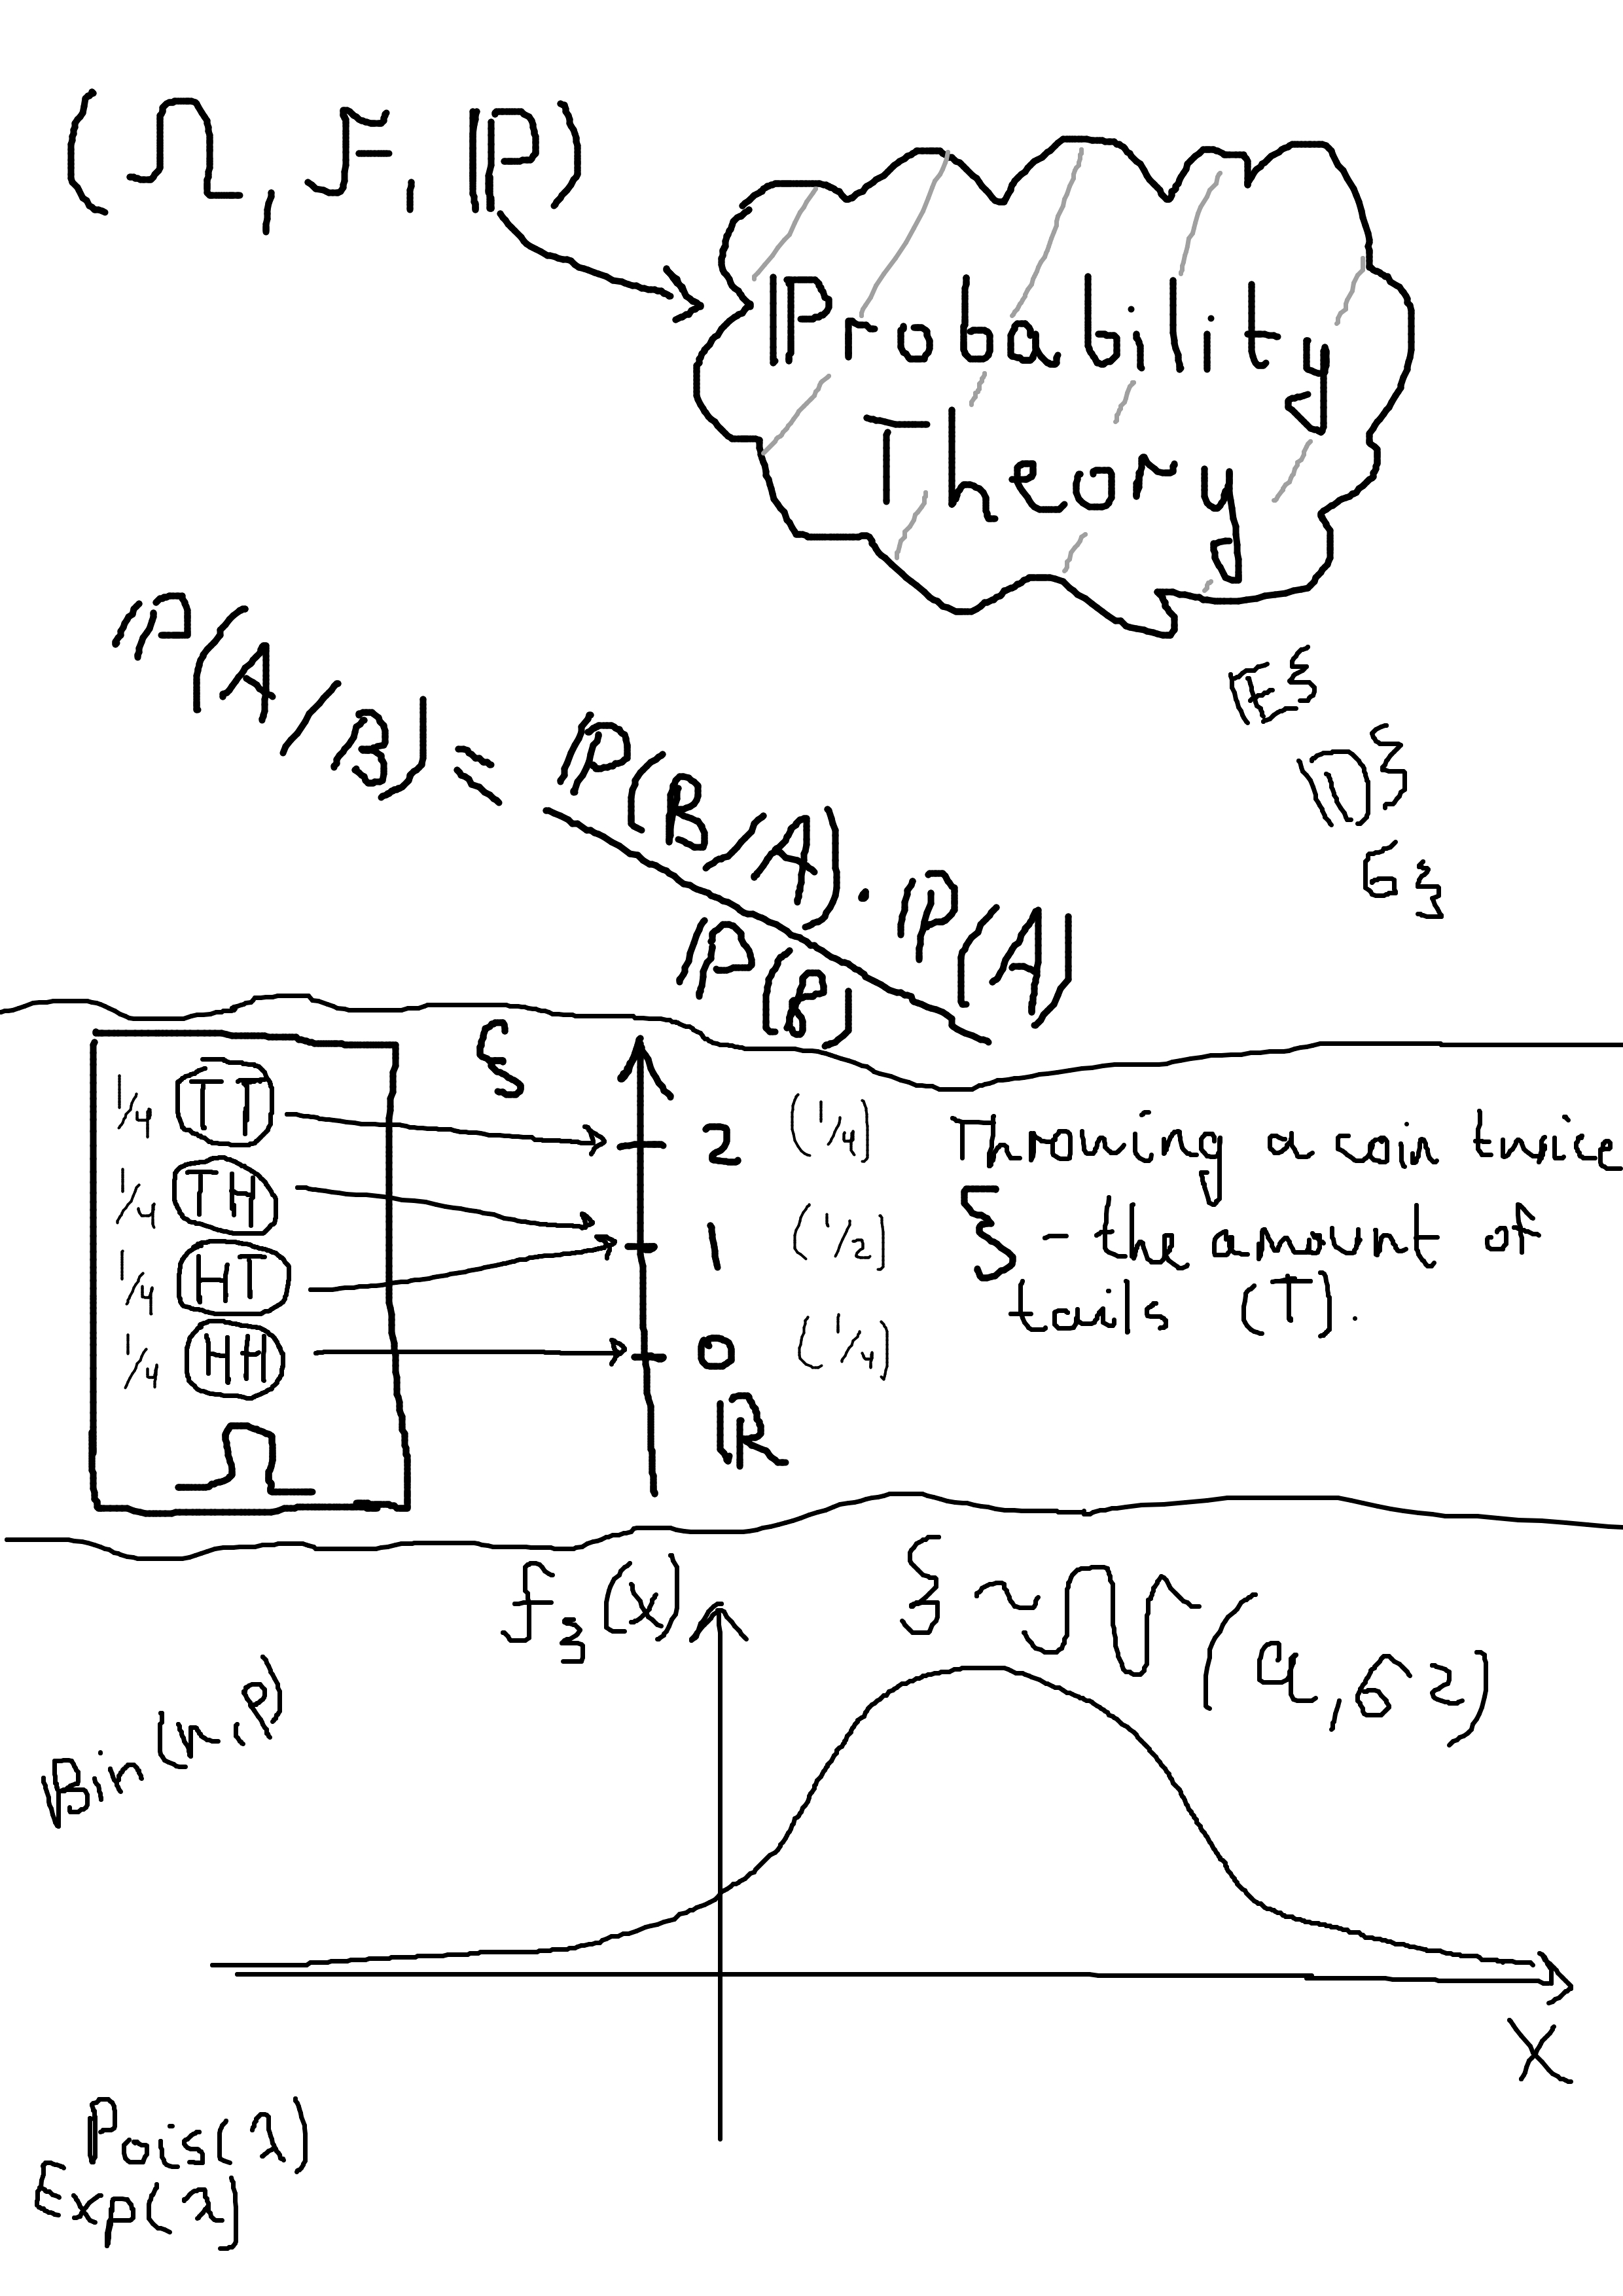
\includepdf{preview.jpg}
\tableofcontents
\newpage

\iffalse %I really don't know if I need to rewrite topology
\section{Деякі відомості з топології}
\subsection{Інше означення неперервності}
\begin{proposition}
Задано функцію $f \colon \mathbb{R}^n \to \mathbb{R}^n$.\\
$f \in C(\mathbb{R}^n) \iff \forall U$ -- відкрита: $f^{-1}(U)$ -- відкрита.
\end{proposition}

\begin{proof}
\rightproof Дано: $f \in C(\mathbb{R}^n)$. Оберемо $U$ відкриту множину. Тепер оберемо точку $x_0 \in f^{-1}(U) \implies f(x_0) \in U$. Точка $f(x_0)$ -- внутрішня, тому звідси існує окіл $U_\varepsilon(f(x_0)) \subset U$. Водночас для цього $\varepsilon > 0$ існує $\delta > 0$ такий, що $\forall x \in U_\delta(x_0) \implies f(x) \in U_\varepsilon(f(x_0))$, тобто інакше $f(U_\delta(x_0)) \subset U_\varepsilon(f(x_0))$. Звідси випливає, що $U_\delta(x_0) \subset f^{-1}(U_\varepsilon (f(x_0))) \subset f^{-1}(U)$. Отже, $f^{-1}(U)$ -- відкрита.
\bigskip \\
\leftproof Дано: $\forall U$ -- відкрита: $f^{-1}(U)$ -- відкрита. Нехай $x_0 \in \mathbb{R}^n$ та $\varepsilon > 0$ задані. Розглянемо відкритий окіл $U_\varepsilon(f(x_0))$. Оскільки це відкрита множина, то $f^{-1}(U_\varepsilon(f(x_0)))$ -- також відкрита множина. Оскільки $x_0 \in f^{-1}(U_\varepsilon(f(x_0)))$, то тоді існує окіл $U_\delta \subset f^{-1}(U_\varepsilon(f(x_0))) \implies f(U_\delta) \subset U_\varepsilon(f(x_0))$. Це вкладення можна переписати так: існує $\delta > 0$ так, що $\forall x \in \mathbb{R}^n: \|x - x_0 \| < \delta \implies \|f(x) - f(x_0)\| < \varepsilon$. Це означає неперервність в точці $x_0$.
\end{proof}

\begin{proposition}
Задано функцію $f \colon \mathbb{R}^n \to \mathbb{R}^n$.\\
$f \in C(\mathbb{R}^n) \iff \forall V$ -- замкнена: $f^{-1}(V)$ -- замкнена.\\
\textit{Вказівка: $V$ -- замкнена, тобто $\mathbb{R}^n \setminus V$ -- відкрита.}
\end{proposition}

\subsection{Корисні леми}
\begin{lemma}
Для всіх $r \in [0,1] \cap \mathbb{Q}$ задамо відкриті множини $V_r \subset \mathbb{R}^n$, для яких виконується $\Cl(V_r) \subset V_{r'}$ при $r < r'$. Тоді існує функція $f \colon \mathbb{R}^n \to [0,1],\ f \in C(\mathbb{R}^n)$, для якої $f(\vec{x}) = 0, x \in V_0$ та $f(\vec{x}) = 1, x \notin V_1$.
\begin{figure}[H]
\centering
\begin{tikzpicture}
\draw (0,0) rectangle (6,4) node[anchor = north east] {$X$};
\filldraw[fill = red!0, draw = red] (0.5,0.2) rectangle (5,3.8) node[scale=0.6, anchor = north east]{$V_{1}$};
\filldraw[fill = red!20, draw = red] (0.8,0.5) rectangle (4.2,3.5) node[scale=0.6, anchor = north east]{$V_{8/9}$};
\filldraw[fill = red!40, draw = red] (1,1.3) rectangle (4,3.1) node[scale=0.6, anchor = north east]{$V_{3/5}$};
\filldraw[fill = red!60, draw = red] (1.5,1.5) rectangle (3.5,3) node[scale=0.6, anchor = north east]{$V_{1/2}$};
\filldraw[fill = red!80, draw = red] (2,1.7) rectangle (2.5,2.5) node[scale=0.6, anchor = north east]{$V_0$};
\end{tikzpicture}
\caption*{Схематична картина умови $\Cl(V_r) \subset V_{r'}$ при $r < r'$.}
\end{figure}
\end{lemma}

\begin{proof}
Визначимо функцію $f \colon \mathbb{R}^n \to [0,1]$ ось таким чином: $f(\vec{x}) = \begin{cases} 1, & \vec{x} \notin V_1 \\ \inf_{\vec{x} \in V_r} \{r\}, & \vec{x} \in V_1 \end{cases}$. \\
Зауважимо, що в нашому випадку, що при $\vec{x} \in V_0$ маємо $f(\vec{x}) = 0$. Дійсно, оскільки $\vec{x} \in V_0$, то звідси $\vec{x} \in V_r, \forall r \in [0,1] \cap \mathbb{Q}$, найменше можливе значення -- це нуль. Тож звідси $f(\vec{x}) = 0$.
Ми спочатку доведемо, що прообрази $f^{-1}([0,a))$ та $f^{-1}((a,1])$ будуть відкритими для кожного $a \in [0,1]$. Множини $[0,a),(a,1]$ є відкритими на відрізку $[0,1]$.\\
$f^{-1}([0,a)) = \displaystyle\bigcup_{r < a} V_r$. \\
Дійсно, маємо $x \in f^{-1}([0,a)) \iff f(x) < a \iff \displaystyle\inf_{x \in V_r} \{r\} < a \iff x \in V_r$ для деякого $r < a$.\\
Ми отримали, що $f^{-1}([0,a))$ -- відкрита як зліченне об'єднання відкритих.\\
$f^{-1}((a,1]) = \displaystyle\bigcup_{r > a} (X \setminus \Cl(V_r))$.\\
Маємо $x \in f^{-1}((a,1]) \implies a < f(x) \leq 1 \implies x \notin V_r$ для деякого $r > a$, але тоді $x \notin \Cl(V_{r'})$ для $r' < r$ (ми можемо знайти $r'$ так, щоб $r' \in (a,r)$). Тобто $x \in X \setminus \Cl(V_{r'})$ при деякому $r' > a$.\\
Якщо $x \notin \Cl(V_r)$ при деякому $r > a$, то отримаємо $f(x) > a$. Адже якби $f(x) \leq a$, то $x \in V_{r'}$ при $r' \leq a < r$, але тоді $\Cl(V_{r'}) \subset V_r \subset \Cl(V_r)$. Таким чином, $f(x) > a \implies x \in f^{-1}((a,1])$.\\
Оберемо довільний відкритий інтервал $(a,b) \subset [0,1]$. Тоді звідси $(a,b) = [0,b) \cap (a,1]$, а далі прообраз $f^{-1}((a,b)) = f^{-1}([0,b)) \cap f^{-1}((a,1])$ буде відкритою.\\
Якщо $U$ -- довільна відкрита на $[0,1]$, то звідси $U = \displaystyle\bigcup (a,b) \cup \displaystyle\bigcup [0,c) \cup \displaystyle\bigcup (d,1]$, тому прообраз\\
$f^{-1}(U) = \displaystyle\bigcup f^{-1}((a,b)) \cup \bigcup f^{-1}([0,c)) \cup \bigcup f^{-1}((d,1])$ -- відкрита.
\end{proof}

\begin{lemma}
Задано $(X,\tau)$ -- нормальний топологічний простір. Припустимо, що $A$ -- замкнена та $U$ -- відкрита, де $A \subset U$. Тоді існує $V$ -- відкрита множина, для якої $A \subset V, \Cl(V) \subset U$.
\begin{figure}[H]
\centering
\begin{tikzpicture}
\draw (0,0) rectangle (2,1) node[anchor = north east] {$A$};
\draw[dashed] (-1,-1) rectangle (3,2) node[anchor = north east] {$U$};
\draw[dashed,red] (1,0.5) circle (1.4cm) node at (1,1.5) {$V$};
\end{tikzpicture}
\caption*{Тобто між замкненою та відкритою множинах можна підібрати проміжну відкриту множину, яка містить замкнену, а замикання міститься в відкритій.}
\end{figure}
\end{lemma}

\begin{proof}
Оберемо $A, X \setminus U$ -- обидва замкнені множини. За нормальністю, існують відкриті множини $V,W$, що неперетинні, для яких $V \supset A, W \supset X \setminus U$. Тобто $V \supset A$ та $X \setminus W \subset U$. Із того, що $V,W$ -- неперетинні, тобто $V \cap W = \emptyset$, випливає $V \subset X \setminus W$. Маємо ланцюг $A \subset V \subset X \setminus W \subset U$. Оскільки $V \subset X \setminus W$, то тоді й $\Cl(V) \subset \Cl(X \setminus W) = X \setminus W$. Власне, звідси довели: $A \subset V, \Cl(V) \subset U$.
\end{proof}

\begin{theorem}[Лема Урисона]
Нехай $A,B \subset \mathbb{R}^n$ -- замкнені та неперетинні множини. Тоді існує функція $f \colon \mathbb{R}^n \to [0,1],\ f \in C(\mathbb{R}^n)$, для якої $f(\vec{x}) = 0, \vec{x} \in A$ та $f(\vec{x}) = 1, \vec{x} \in B$.
\begin{figure}[H]
\centering
\begin{tikzpicture}
\draw (0,0) rectangle (8,6) node[anchor = north east] {$\mathbb{R}^n$};
\filldraw[fill = red!0, draw = red] (0.2,0.2) rectangle (4.5,4.5) node[anchor = north east] {$V_{1}$};
\filldraw[fill = red!20, draw = red] (0.5,0.4) rectangle (4,4) node[anchor = north east] {$V_{8/9}$};
\filldraw[fill = red!40, draw = red] (0.6,0.6) rectangle (3.3,3.4) node[anchor = north east] {$V_{3/5}$};
\filldraw[fill = red!60, draw = red] (0.8,0.7) rectangle (2.8,2.9) node[anchor = north east] {$V_{1/2}$};
\filldraw[fill = red!80, draw = red] (0.9,0.9) rectangle (2.4,2.4) node[anchor = north east] {$V_0$};
\filldraw[fill = blue, draw = black] (1,1) rectangle (2,2) node[anchor = north east] {$A$};
\filldraw[fill = blue, draw = black] (5,4) rectangle (7,5) node[anchor = north east] {$B$};
\end{tikzpicture}
\caption*{Схематичний план доведення.}
\end{figure}
\end{theorem}

\begin{proof}
Ідея доведення полягає в наступному: ми хочемо побудувати відкриті множини $V_r \subset \mathbb{R}^n, r \in [0,1] \cap \mathbb{Q}$, що задовольняє таким вимогам:\\
1) $A \subset V_0$;\\
2) $B \subset \mathbb{R}^n \setminus V_1$;\\
3) $r < r' \implies \Cl(V_r) \subset V_{r'}$.\\
Оскільки $[0,1] \cap \mathbb{Q}$ -- зліченна множина, то ми маємо послідовність $r_1,r_2,r_3,\dots,r_n,\dots$ різних раціональних чисел. Не втрачаючи загальності, $r_1 = 1, r_2 = 0$, а всі решта $0 < r_n < 1$.\\
\textit{База індукції} (їх будуть дві): треба побудувати $V_{r_1} = V_1$ та $V_{r_2} = V_0$. Покладемо $V_1 = \mathbb{R}^n \setminus B$ -- уже відкрита. Оскільки $A \subset \mathbb{R}^n, V_1 \subset \mathbb{R}^n$ -- одна замкнена, інша відкрита, то за другою лемою, існує відкрита множина $V_0$, для якої $A \subset V_0$ та $\Cl(V_0) \subset V_1$. Уже маємо $V_{r_1},V_{r_2}$, які задовольняють вимогам 1),2),3).\\
Для всіх інших $V_{r_n}$ нам досить буде довести 3).\\
\textit{Припущення індукції}: $V_{r_3},\dots,V_{r_n}$ побудовані так, що задовольняють нашим умовам вище.\\
\textit{Крок індукції}: побудуємо $V_{r_{n+1}}$. Із нашої послідовності $r_1,r_2,\dots,r_n$ оберемо два якнайближчих числа $r_i,r_j$, щоб $r_i < r_{n+1} < r_j$. Нам досить довести, що $\Cl(V_{r_i}) \subset V_{r_{n+1}},\ \Cl(V_{r_{n+1}}) \subset V_{r_j}$.\\
Зауважимо, що $\Cl(V_{r_i})$ та $V_{r_j}$ -- відповідно замкнена та відкрита множини. Тоді за другою лемою, існує відкрита множина (яку як раз-таки позначимо й за $V_{r_{n+1}}$), для якої справджуються ці два вкладення. \\
МІ доведено.\\
Значить, за першою лемою, існує неперервна функція $f \colon \mathbb{R}^n \to [0,1]$, для якої $f(\vec{x}) = 0, \vec{x} \in V_0$ та $f(\vec{x}) = 1, \vec{x} \notin V_1$. За умовами 1),2), отримаємо $f(\vec{x}) = 0, \vec{x} \in A$ та $f(\vec{x}) = 1, \vec{x} \in B$.
\end{proof}

\begin{remark}
Лему Урисона можна дещо узагальнити. Якщо маємо $A,B \subset \mathbb{R}^n$ -- неперетинні замкнені, то ми можемо навіть підібрати функцію $g \colon \mathbb{R}^n \to [a,b]$, для якої $f(\vec{x}) = a, \vec{x} \in A$ та $f(\vec{x}) = b, \vec{x} \in B$. Тобто не обов'язково на відрізку $[0,1]$, а на будь-якому.\\
\textit{Вказівка: $h \colon [0,1] \to [a,b],\ h(\vec{x}) = a + (b-a)\vec{x}$.}
\end{remark}

\subsection{Теорема Тітце}
\begin{lemma}
Задана $A \subset \mathbb{R}^n$ -- замкнена множина та $f \colon A \to \mathbb{R}$ -- неперервна функція, причому $\exists C > 0: \forall \vec{x} \in A: |f(\vec{x})| \leq C$. Тоді існує неперервна функція $g \colon \mathbb{R}^n \to \mathbb{R}$, для якої $\forall \vec{x} \in \mathbb{R}^n: |g(\vec{x})| \leq \dfrac{1}{3}C$ та $\forall \vec{x} \in A: |f(\vec{x}) - g(\vec{x})| \leq \dfrac{2}{3}C$.
\end{lemma}

\begin{proof}
Розглянемо прообрази $Y = f^{-1}\left(\left[\dfrac{1}{3}C,C\right]\right)$ та $Z = f^{-1}\left(\left[-C, -\dfrac{1}{3}C \right]\right)$. Обидві множини $Y,Z$ -- замкнені, оскільки в прообраз (неперервної функції) передаємо замкнені множини в $\mathbb{R}$. Також оскільки ці відрізки неперетинні, то $Y,Z$ також неперетинні. Значить, за лемою Урисона (трошки в загальній формі), існує функція $g \colon \mathbb{R}^n \to \left[-\dfrac{1}{3}C, \dfrac{1}{3}C\right]$, де $g|_Y = \dfrac{1}{3}C$ та $g|_Z = -\dfrac{1}{3}C$. Зважаючи на область значень, маємо $|g(\vec{x})| \leq \dfrac{1}{3}C$. \\
Залишилося довести, що $|f(\vec{x}) - g(\vec{x})| \leq \dfrac{2}{3}C$. Розглянемо три випадки:\\
$\vec{x} \in Y$, тоді $g(\vec{x}) = \dfrac{1}{3}C$ та $\dfrac{1}{3}C \leq f(\vec{x}) \leq C$, тож звідси $0 \leq f(\vec{x}) - g(\vec{x}) \leq \dfrac{2}{3}C$;\\
$\vec{x} \in Z$, тоді $g(\vec{x}) = -\dfrac{1}{3}C$ та $-C \leq f(\vec{x}) \leq -\dfrac{1}{3}C$, тож звідси $-\dfrac{2}{3}C \leq f(\vec{x}) - g(\vec{x}) \leq 0$;\\
$\vec{x} \notin Y \sqcup Z$, тоді $|f(\vec{x})| \leq \dfrac{1}{3}C$ та $|g(\vec{x})| \leq \dfrac{1}{3}C$, тож за нерівністю трикутника $|f(\vec{x}) - g(\vec{x})| \leq \dfrac{2}{3}C$.
\end{proof}

\begin{theorem}[Теорема Тітце]
Задана $A \subset \mathbb{R}^n$ -- замкнена множина та $f \colon A \to [a,b]$ -- неперервна функція. Тоді існує неперервна функція $\overline{f} \colon \mathbb{R}^n \to [a,b]$ -- розширення $f$, тобто $\overline{f}|_{A} = f$.
\end{theorem}

\begin{proof}
За умовою, функція $f$ повертає значення відрізка $[a,b]$, тому маємо $\forall \vec{x} \in A: |f(\vec{x})| \leq C$. Ми стверджуємо, що для кожного $n \in \mathbb{N}$ існує неперервна функція $g_n \colon X \to \mathbb{R}$, що задовольняє таким умовам:
\begin{enumerate}[nosep,wide=0pt,label={\arabic*)}]
\item $\forall \vec{x} \in X: |g_n(\vec{x})| \leq \dfrac{1}{3} \left( \dfrac{2}{3}\right)^{n-1} C$;
\item $\forall \vec{x} \in A: \displaystyle\left| f(\vec{x}) - \sum_{k=1}^n g_k(\vec{x}) \right| \leq \left( \dfrac{2}{3} \right)^n C$.
\end{enumerate}
\textit{База індукції}: при $n = 1$ така функція $g_1$ існує за попередньою лемою.\\
\textit{Припущення індукції}: уже побудовані функції $g_1,\dots,g_n$, що задовольняють вимогам вище.\\
\textit{Крок індукції}: позначмио функцію $\varphi(\vec{x}) = \displaystyle f(\vec{x}) - \sum_{k=1}^n g_k(\vec{x})$. Маємо функцію $\varphi \colon A \to \mathbb{R}$, яка неперервна (як сума неперервних) та обмежена ось так: $\forall \vec{x} \in A: |\varphi(\vec{x})| \leq \left( \dfrac{2}{3} \right)^n C$. Звідси за лемою вище існує функція $g_{n+1} \colon X \to \mathbb{R}$, що неперервна та задовольняє оцінкам $|g_{n+1}(\vec{x})| \leq \dfrac{1}{3} \left[ \left(\dfrac{2}{3}\right)^n C \right]$ та $|\varphi(\vec{x}) - g_{n+1}(\vec{x})| = \displaystyle\left| f(\vec{x}) - \sum_{k=1}^{n+1} g_k(\vec{x}) \right| \leq \left( \dfrac{2}{3} \right)^{n+1}C$.\\
МІ доведено. \\
Тепер визначимо функцію $\overline{f}_{\infty} \colon X \to \mathbb{R}$ ось таким чином: $\overline{f}_\infty(\vec{x}) = \displaystyle\sum_{k=1}^\infty g_k(\vec{x})$. Дана функція визначена коректно (тобто ряд при кожному $\vec{x} \in \mathbb{R}^n$ збіжний в силу оцінки $|g_n(\vec{x})| \leq \dfrac{1}{3} \left( \dfrac{2}{3}\right)^{n-1}C$; навіть рівномірно збіжний ряд за мажорантою Ваєрштраса). \\
Доведемо, що дана функція буде неперервною. Для цього позначимо $\overline{f}_n(\vec{x}) = \displaystyle\sum_{k=1}^n g_k(\vec{x})$; ці функції є неперервними як сума неперервних. Далі зазначимо, що $\overline{f}_n$ збігається рівномірно до $\overline{f}_\infty$ в силу рівномірної збіжності ряду. Отже, $\overline{f}_\infty$ буде точно неперервною.\\
Причому зазначимо, що $\forall \vec{x} \in A: \overline{f}_\infty(\vec{x}) = f(\vec{x})$. Справді, маємо оцінку:\\
$\forall \vec{x} \in A: \displaystyle\left| f(\vec{x}) - \sum_{k=1}^n g_k(\vec{x}) \right| \leq \left(\dfrac{2}{3}\right)^n C \overset{n \to \infty}{\implies} f(\vec{x}) = \overline{f}_\infty(\vec{x})$.\\
Утім все ж таки ми знайшли функцію $\overline{f}_\infty \colon X \to \mathbb{R}$, а нам потрібна функція $\overline{f} \colon X \to [a,b]$. Питань нема, визначимо її ось таким чином: $\overline{f}(\vec{x}) = \begin{cases} \overline{f}_\infty(\vec{x}), & \vec{x} \in \overline{f}_\infty^{-1}([a,b]) \\ a, & \vec{x} \in \overline{f}_\infty^{-1}((-\infty,a)) \\ b, & \vec{x} \in \overline{f}_\infty^{-1}((b,+\infty)) \end{cases}$. Така функція буде неперервною (в принципі, зрозуміло), а також $\overline{f}|_A = f$. Дійсно, якщо $\vec{x} \in A$, то тоді $f(\vec{x}) = \overline{f}_\infty(\vec{x}) \in [a,b]$, тобто $\vec{x} \in \overline{f}_\infty^{-1}([a,b])$. Значить, $\overline{f}(\vec{x}) = \overline{f}_\infty(\vec{x}) = f(\vec{x})$.
\end{proof}
\noindent
Це ми довели лише теорему Тітце для функції, що приймають значення лише на деякому відрізку. Трошки розшириимо клас функцій.

\begin{theorem}[Теорема Тітце (розширення)]
Задана $A \subset X$ -- замкнена множина та $f \colon A \to \mathbb{R}$ -- неперервна функція. Тоді існує неперервна функція $\overline{f} \colon \mathbb{R}^n \to \mathbb{R}$ -- розширення $f$, тобто $\overline{f}|_{A} = f$.
\end{theorem}

\begin{proof}
Ми будемо доводити розширення теореми для випадку, коли задана функція $f \colon A \to (-1,1)$. Оскільки маємо $(-1,1) \subset [-1,1]$, то за теоремою вище, існує функція $\overline{f} \colon X \to [-1,1]$ -- неперервна та $\overline{f}_A = f$. На жаль, це ще не все, бо нам треба функція $\overline{g} \colon A \to (-1,1)$, у нас там проблемки в точках $\{-1,1\}$.\\
Проте якщо взяти множину $B = \overline{f}^{-1}(\{-1,1\})$, що буде замкненою та $A \cap B = \emptyset$, то за лемою Урисона існуватиме функція $\varphi \colon X \to [0,1]$, де $\varphi|_A = 1$ та $\varphi|_B = 0$. Тепер визначимо функцію $\overline{g}(x) = \overline{f}(x) \cdot \varphi(x)$. Функція $g \colon X \to (-1,1)$, неперервна як добуток та $\overline{g}|_A = f$.\\
Далі ми згадуємо той факт, що $(-1,1) \cong \mathbb{R}$ -- отримаємо бажане.
\end{proof}
\newpage
\fi

\section{Кратні інтеграли}
\subsection{Бруси, розбиття, підрозбиття}
\begin{definition}
\textbf{Прямокутним паралелепіпедом в} $\mathbb{R}^m$ або \textbf{$m$-вимірних брусом} називають множину
\begin{align*}
Q = [a_1,b_1] \times \dots \times [a_m,b_m].
\end{align*}
\begin{figure}[H]
\centering
\begin{tikzpicture}[scale = 0.6]
\filldraw[draw = blue, fill = blue!50] (0,0) rectangle (3,2);
\end{tikzpicture}
\qquad
\begin{tikzpicture}[scale = 0.6]
\fill[blue!50] (0,0.6)--(2,0.6)--(3,2.1)--(1,2.1)--cycle;
\fill[blue!50] (2,0.6)--(2,-0.4)--(3,1.1)--(3,2.1);
\fill[blue!50] (0,0.6)--(0,-0.4)--(2,-0.4)--(2,0.6);
\draw[blue] (0,0.6)--(2,0.6)--(3,2.1)--(1,2.1)--cycle;
\draw[blue] (2,0.6)--(2,-0.4)--(3,1.1)--(3,2.1);
\draw[blue] (0,0.6)--(0,-0.4)--(2,-0.4);
\end{tikzpicture}
\caption*{Брусом в $\mathbb{R}^2$ буде прямокутник; брусом в $\mathbb{R}^3$ буде прямокутний паралелепіпед.}
\end{figure}
\textbf{Діаметром бруса} $Q$ називають число
\begin{align*}
d(Q) = \sup_{\vec{x},\vec{y} \in Q} \Norm{\vec{x}-\vec{y}}.
\end{align*}
У нашому випадку $d(Q) = \sqrt{(b_1-a_1)^2 + \dots + (b_m-a_m)^2}$ -- власне кажучи, діагональ бруса.\\
\textbf{Об'ємом} або \textbf{мірою} бруса $Q$ називається додатне число
\begin{align*}
m(Q) = \prod_{k=1}^m (b_k-a_k).
\end{align*}
\begin{figure}[H]
\centering
\begin{tikzpicture}
\filldraw[draw = blue, fill = blue!50] (0,0) rectangle (4,2);
\end{tikzpicture}
\caption*{Випадок $\mathbb{R}^2$ -- прямокутник $Q = [0,4] \times [0,2]$ з діаметром $d(Q) = 2 \sqrt{5}$ та мірою $m(Q) = 4 \cdot 2 = 8$.}
\end{figure}
\end{definition}
\noindent
Далі нехай $Q = \displaystyle\prod_{k=1}^m [a_k,b_k]$ -- брус. Ми розглянемо розбиття $\lambda_k = \{x_k^0, x_k^1,\dots,x_k^{n_k} \}$ відрізка $[a_k,b_k]$ для кожного $k = \overline{1,m}$. Нехай $\Delta x_k^v = x_k^{v} - x_k^{v-1}$, де $v = \overline{1,n_k}$.\\
Після такого розбиття ми отримаємо набір брусів $Q(v_1,\dots,v_m) = \displaystyle\prod_{k=1}^m [x_{k}^{v_k-1}, x_k^{v_k}]$, об'єм якого $m(Q(v_1,\dots,v_m)) = \displaystyle\prod_{k=1}^m \Delta x_k^{v_k}$.

\begin{figure}[H]
\centering
\begin{tikzpicture}
\filldraw[draw = blue, fill = blue!50] (0,0) rectangle (4,2);
\foreach \i in {1,2,3} {
	\draw (\i,0)--(\i,2);
	}
\foreach \i in {0.5,1.5} {
	\draw (0,\i)--(4,\i);
	}
\end{tikzpicture}
\caption*{Випадок $\mathbb{R}^2$ -- відрізок $[0,4]$ має розбиття $\{0,1,2,3,4\}$ та відрізок $[0,2]$ має розбиття $\{0,0.5,1.5,2\}$. Після розбиття ми отримали набір прямокутників.}
\end{figure}

\begin{definition}
Цей набір брусів $\lambda = \{Q(v_1,\dots,v_m)\}$ називається \textbf{розбиттям бруса} $Q$.\\
\textbf{Діаметром розбиття} $\lambda$ називається число
\begin{align*}
|\lambda| = \max_{\substack{1 \leq v_k \leq n_k \\ 1 \leq k \leq m}} d(Q(v_1,\dots,v_m))
\end{align*}
По суті кажучи, діаметр розбиття означає шукати найбільшу діагональ бруса.
\end{definition}

\begin{remark}
$\displaystyle\sum_{\substack{1 \leq v_k \leq n_k \\ 1 \leq k \leq m}} m(Q(v_1,\dots,v_m)) = m(Q)$.\\
Дійсно, зауважимо спочатку, що $\displaystyle\sum_{v=1}^{n_k} \Delta x_k^{v} = b_k-a_k$. А далі маємо такий ланцюг рівностей:\\
$\displaystyle\sum_{\substack{1 \leq v_k \leq n_k \\ 1 \leq k \leq m}} m(Q(v_1,\dots,v_m)) = \sum_{\substack{1 \leq v_k \leq n_k \\ 1 \leq k \leq m}} \Delta x_1^{v_1} \dots \Delta x_m^{v_m} = \\ = \textcolor{red}{\Delta x_1^1} \sum_{\substack{1 \leq v_k \leq n_k \\ 2 \leq k \leq m}} \Delta x_2^{v_2} \dots \Delta x_m^{v_m} + \dots + \textcolor{red}{\Delta x_1^{n_1}} \sum_{\substack{1 \leq v_k \leq n_k \\ 2 \leq k \leq m}} \Delta x_2^{v_2} \dots \Delta x_m^{v_m} = \\ = \sum_{\substack{1 \leq v_k \leq n_k \\ 2 \leq k \leq m}} \Delta x_2^{v_2} \dots \Delta x_m^{v_m} (\textcolor{red}{\Delta x_1^1 + \dots + \Delta x_1^{n_1}}) = (b_1-a_1) \sum_{\substack{1 \leq v_k \leq n_k \\ 2 \leq k \leq m}} \Delta x_2^{v_2} \dots \Delta x_m^{v_m} = \\
= \dots = (b_1-a_1)(b_2-a_2) \dots (b_m-a_m) = m(Q)$.
\end{remark}

Тепер з'ясуємо, як отримати підрозбиття. Маємо $Q$ -- деякий брус та розбиття $\lambda$. Його ми отримали в результаті розбиття кожного відрізку. Щоб отримати підрозбиття $\lambda'$ розбиття $\lambda$, ми запишемо підрозбиття $\lambda'_k$ розбиття кожного відрізка $\lambda_k$ (ми це робили додаванням точок).\\
\begin{figure}[H]
\centering
\begin{tikzpicture}
\filldraw[draw = blue, fill = blue!50] (0,0) rectangle (4,2);
\foreach \i in {1,2,3} {
	\draw (\i,0)--(\i,2);
	}
\foreach \i in {0.5,1.5} {
	\draw (0,\i)--(4,\i);
	}
\end{tikzpicture}
\qquad
\begin{tikzpicture}
\filldraw[draw = blue, fill = blue!50] (0,0) rectangle (4,2);
\foreach \i in {1,2,3} {
	\draw (\i,0)--(\i,2);
	}
\foreach \i in {0.5,1.5,2.5} {
	\draw[red] (\i,0)--(\i,2);
	}
\foreach \i in {0.5,1.5} {
	\draw (0,\i)--(4,\i);
	}
\foreach \i in {1} {
	\draw[red] (0,\i)--(4,\i);
	}
\end{tikzpicture}
\end{figure}
З'ясуємо, що буде відбуватись з кожним брусом $Q_1(v_1,\dots,v_m) = [x_k^{v_1},x_k^{v_1+1}] \times \dots \times [x_k^{v_m}, x_k^{v_m+1}]$.\\
І. Жодний відрізок, що бере участь в $Q(v_1,\dots,v_m)$, не підрозбивається. Тоді нічого з ним не буде.\\
II. Знайдеться відрізок, що бере участь в $Q(v_1,\dots,v_m)$, який підрозбивається. Не втрачаючи загальності, скажімо $[x_k^{v_1},x_k^{v_1+1}] = [x_k^{v_1}, y_0] \cup [y_0, y_1] \cup \dots \cup [y_p, x_k^{v_1+1}]$. У цьому випадку $y_0,y_1,\dots,y_p$ будуть точками, що були додані під час підзробиття відрізка. Тоді\\
$Q(v_1,\dots,v_m) = [x_k^{v_1},x_k^{v_1+1}] \times \dots \times [x_k^{v_m}, x_k^{v_m+1}] = \\
= ([x_k^{v_1}, y_0] \cup [y_0, y_1] \cup \dots \cup [y_p, x_k^{v_1+1}]) \times [x_k^{v_2}, x_k^{v_2+1}] \times \dots \times [x_k^{v_m}, x_k^{v_m+1}] = \\
= ([x_k^{v_1},y_0] \times [x_k^{v_2}, x_k^{v_2+1}] \times \dots \times [x_k^{v_m}, x_k^{v_m+1}]) \cup \dots \cup ([y_p,x_k^{v_k+1}] \times [x_k^{v_2}, x_k^{v_2+1}] \times \dots \times [x_k^{v_m}, x_k^{v_m+1}]) = \\
= Q_1 \cup \dots \cup Q_p$.\\
Ми тіпа розкриваємо дужки з точки зору теорії множин.\\
Таким чином, отримали, що брус розіб'ється на підбруси. Причому згідно зі зауваженням вище, $\displaystyle\sum m(Q_i) = m(Q(v_1,\dots,v_m))$.\\
Саме за таким процесом, розбиваючи $\lambda$, отримаємо підрозбиття $\lambda'$.

\subsection{Кратні інтеграли по брусу}
Надалі вводиться позначення $\omega(\lambda) = \{ (v_1,\dots,v_m) | 0 \leq v_k \leq n_k-1, 1 \leq k \leq m \}$.

\begin{definition}
Задано $Q$ -- брус та функцію $f \colon Q \to \mathbb{R}$ -- обмежена на $Q$ та $\lambda$ -- розбиття бруса.\\
\textbf{Нижньою сумою Дарбу} для розбиття $\lambda$ та функції $f$ називається сума
\begin{align*}
L(f,\lambda) = \sum_{(v_1,\dots,v_m) \in \omega(\lambda)} \inf_{\vec{x} \in Q(v_1,\dots,v_m)} f(\vec{x}) \cdot m(Q(v_1,\dots,v_m)).
\end{align*}
\textbf{Верхньою сумою Дарбу} для розбиття $\lambda$ та функції $f$ називається сума
\begin{align*}
U(f,\lambda) = \sum_{(v_1,\dots,v_m) \in \omega(\lambda)} \sup_{\vec{x} \in Q(v_1,\dots,v_m)} f(\vec{x}) \cdot m(Q(v_1,\dots,v_m)).
\end{align*}
\end{definition}

\begin{definition}
Набір точок $\{ \vec{\xi}(v_1,\dots,v_m) | (v_1,\dots,v_m) \in \omega(\lambda) \} = \{ \vec{\xi} (v_1,\dots,v_m) \}$ назвемо \textbf{набором, що відповідає розбиттю} $\lambda$. Тут всі $\vec{\xi}(v_1,\dots,v_m) \in Q(v_1,\dots,v_m)$.
\end{definition}

\begin{definition}
Задано $Q$ -- брус та функцію $f \colon Q \to \mathbb{R}$ та $\lambda$ -- розбиття бруса.\\
\textbf{Інтегральною сумою} для розбиття $\lambda$ з наборами $\{ \vec{\xi}(v_1,\dots,v_m) \}$ функції $f$ називається сума
\begin{align*}
\sigma(f,\lambda, \{ \vec{\xi}(v_1,\dots,v_m) \}) = \sum_{(v_1,\dots,v_m) \in \omega(\lambda)} f(\vec{\xi}(v_1,\dots,v_m)) \cdot m(Q(v_1,\dots,v_m))
\end{align*}
\end{definition}

%Fucking embarrassing
\iffalse
\begin{figure}[H]
\centering
\includegraphics[scale=1]{RiemannSumR2.png}
\end{figure}
\fi

\begin{figure}[H]
\centering
\begin{tikzpicture}
\draw[->] (-0.5,0)--(4,0) node[anchor = north west] {$y$};
\draw[->] (-0.5,0)--(-0.5,3) node[anchor = south east] {$z$};
\draw[->] (-0.5,0)--(-3,-2.5) node[anchor = north] {$x$};
\draw (1,-0.5)--(3,-0.5)--(2,-2)--(0,-2)--cycle;

\draw[dashed] (0,-2)--(0,-0.5);
\draw[dashed] (2,-2)--(2,0.5);
\draw[dashed] (3,-0.5)--(3,1);
\draw[dashed] (1,-0.5)--(1,2);

\filldraw [draw = red, fill = red!40] plot [smooth cycle] coordinates {(0,-0.5) (0.5,0.25) (1.2,0.5) (2,0.5) (2.3,0.8) (3,1) (2,1.8) (1,2) (0,1)} node[scale=1,red] at (0.2,0.2) {$f$};


%specific part of partition
\fill[blue!20] ({1/3+1},-1.5)--({2/3+1},-1)--({2/3+0.5},-1)--({1/3+0.5},-1.5)--cycle;

%draw a partition
\draw ({1/3},-1.5)--({1/3+2},-1.5);
\draw ({2/3},-1)--({2/3+2},-1);
\draw (0.5,-2)--(1.5,-0.5);
\draw (1,-2)--(2,-0.5);
\draw (1.5,-2)--(2.5,-0.5);

%go up to function
\fill[red] ({1/3+1-0.1},{-1.5+0.25}) circle (1pt);
\draw[red,dashed] ({1/3+1-0.1},{-1.5+0.25})--({1/3+1-0.1},0.9);
\fill[red] ({1/3+1-0.1},0.9) circle (1pt);

\draw[red,->] (-0.5,{-1.5+0.25})--({1/3+1-0.2},{-1.5+0.25}) node[scale=1,red] at (-0.6,{-1.5+0.25-0.2}) {$\xi(v_1,v_2)$};

%rectangle on surface
\draw[blue,dashed] ({1/3+1},0.7)--({2/3+1},{0.7+0.5})--({2/3+0.5},{0.7+0.5})--({1/3+0.5},{0.7})--cycle;
\draw[blue,dashed] ({1/3+1},-1.5)--({1/3+1},0.7);
\draw[blue,dashed] ({2/3+1},-1)--({2/3+1},1.2);
\draw[blue,dashed] ({2/3+0.5},-1)--({2/3+0.5},1.2);
\draw[blue,dashed] ({1/3+0.5},-1.5)--({1/3+0.5},0.7);
\end{tikzpicture}
\caption*{Інтегральна сума для двовимірного бруса $Q$ та відповідно двовимірної функції $f(x,y)$.}
\end{figure}

\begin{definition}
Функція $f$ називається \textbf{інтегрованою за Ріманом}, якщо
\begin{align*}
\exists I \in \mathbb{R}: \forall \varepsilon > 0: \exists \delta(\varepsilon): \forall (\lambda, \vec{\xi}(v_1,\dots,v_m) ): |\lambda| < \delta \implies |\sigma(f,\lambda,\vec{\xi}(v_1,\dots,v_m)) - I| < \varepsilon
\end{align*}
Число $I$ називають \textbf{$m$-кратним інтегралом Рімана}.\\
Позначення: $\displaystyle\int\displaylimits_Q f(\vec{x})\,d\vec{x}$. Часто користуються позначенням $\displaystyle\idotsint_Q f(x_1,\dots,x_m)\,dx_1\,\dots\,dx_m$. У випадку $\mathbb{R}^2$ позначення завжди $\displaystyle\iint_Q f(x,y)\,dx\,dy$. У випадку $\mathbb{R}^3$ позначення завжди $\displaystyle\iiint_Q f(x,y,z)\,dx\,dy\,dz$.
\end{definition}

\begin{example}
Довести, що $f(\vec{x}) = 1$ -- інтегрована на брусі $Q$ та $\displaystyle\int\displaylimits_Q 1\,d\vec{x} = m(Q)$.\\
Дійсно, $\displaystyle\sigma(f,\lambda,\{\vec{\xi}(v_1,\dots,v_m) \}) = \sum_{(v_1,\dots,v_m) \in \omega(\lambda)} m(Q(v_1,\dots,v_m)) = m(Q)$.\\
Отже, $\forall \varepsilon > 0: \exists \delta: \forall (\lambda, \{ \vec{\xi}(v_1,\dots,v_m \}): |\lambda| < \delta \implies |\sigma(f,\lambda,\{ \vec{\xi}(v_1,\dots,v_m) \} - m(Q)| = 0 < \varepsilon$.\\
Отже, $\displaystyle\int\displaylimits_Q 1\,d\vec{x} = m(Q)$.
\end{example}

Всі теореми, твердження, леми та наслідки в даному підрозділі, які залишилися без доведення, вони доводяться \textit{аналогічно як в матані $\mathbb{R}$}. Там дійсно (майже) нічого нового не буде, якщо почати переписувати доведення в багатовимірний випадок.

\begin{theorem}
Задано функцію $f \colon Q \to \mathbb{R}$ -- інтегрована по брусу $Q$. Тоді $f$ -- обмежена на $Q$.
\end{theorem}

\begin{remark}
$L(f,\lambda) \leq \sigma(f,\tau,\{ \vec{\xi}(v_1,\dots,x_m) \}) \leq U(f,\lambda)$.
\end{remark}

\begin{lemma}
Задано функцію $f \colon Q \to \mathbb{R}$ -- обмежена на брусі та будь-яке розбиття $\lambda$. Тоді маємо:\\
$L(f,\lambda) = \displaystyle\inf_{\{ \vec{\xi}(v_1,\dots,x_m) \}} \sigma(f,\tau,\{ \vec{\xi}(v_1,\dots,x_m) \}) \hspace{1cm} U(f,\lambda) = \displaystyle\sup_{\{ \vec{\xi}(v_1,\dots,x_m) \}} \sigma(f,\tau,\{ \vec{\xi}(v_1,\dots,x_m) \})$
\end{lemma}

\begin{lemma}
Задано функцію $f \colon Q \to \mathbb{R}$ -- обмежена на брусі та розбиття $\lambda$. Також задамо підрозбиття $\lambda'$. Тоді $U(f,\lambda) \geq U(f,\lambda')$, а також $L(f,\lambda) \leq L(f,\lambda')$.
\end{lemma}

\begin{lemma}
Задано функцію $f \colon Q \to \mathbb{R}$ -- обмежена на брусі. Візьмемо будь-які два розбиття $\lambda', \lambda''$. Тоді $L(f,\lambda') \leq U(f,\lambda'')$.
\end{lemma}

\begin{definition}
\textbf{Верхнім/нижнім інтегралом Дарбу} будемо називати такі вирази:
\begin{align*}
I^*(f) = \inf_\lambda U(f,\lambda) \hspace{1cm} I_*(f) = \sup_{\lambda} L(f,\lambda)
\end{align*}
\end{definition}

\begin{remark}
Справедлива така нерівність: $I_*(f) \leq I^*(f)$.
\end{remark}

\begin{theorem}[Перший критерій інтегрованості]
Задано функцію $f \colon Q \to \mathbb{R}$, де $Q$ -- брус.\\
$f$ -- інтегрована на $Q \iff f$ -- обмежена на $Q$ та $I_*(f) = I^*(f)$.
\end{theorem}

\begin{theorem}[Другий критерій інтегрованості]
Задано функцію $f \colon Q \to \mathbb{R}$, де $Q$ -- брус.\\
$f$ -- інтегрована на $Q \iff f$ -- обмежена на $Q$ та $\forall \varepsilon > 0: \exists \lambda: U(f,\lambda) - L(f,\lambda) < \varepsilon$.
\end{theorem}

\begin{theorem}
Задано функцію $f \in C(Q)$, де $Q$ -- брус. Тоді $f$ -- інтегрована на $Q$.
\end{theorem}

\begin{theorem}
Задано $f \colon Q \to \mathbb{R}$, де $Q$ -- брус. Припустимо, що $Q = Q_1 \cup Q_2$, де $Q_1,Q_2$ -- бруси, що не мають спільних внутрішніх точок, тобто $\Int(Q_1) \cap \Int(Q_2) = \emptyset$.\\
$f$ -- інтегрована на $Q \iff f$ -- інтегрована на $Q_1$ та $Q_2$.
\end{theorem}

\begin{proof}
Спершу нехай $Q = \displaystyle\prod_{k=1}^m [a_k,b_k]$. Умова $Q = Q_1 \cup Q_2$ та без спільних внутрішніх точок означає, що на $m-1$ відрізків буде ділення на два відрізки (не втрачаючи загальності, це будуть перші $m-1$ штук). Тобто $Q = \displaystyle\prod_{k=1}^{m-1} \left([a_k,c_k] \cup [c_k,b_k]\right) \times [a_m,b_m]$. Це означатиме, що\\
$Q_1 = \displaystyle\prod_{k=1}^{m-1} [a_k,c_k] \times [a_m,b_m],\ Q_2 = \displaystyle\prod_{k=1}^{m-1} [c_k,b_k] \times [a_m,b_m]$.\\
Приступимо до доведення.
\bigskip \\
\rightproof Дано: $f$ -- інтегрована на $Q$. Тоді $f$ -- обмежена на $Q$ (зокрема й на $Q_1,Q_2$), а також $\forall \varepsilon > 0: \exists \lambda: U(f,\lambda) - L(f,\lambda) < \varepsilon$. Маючи розбиття $\lambda$, ми розбиваємо кожний відрізок $[a_k,b_k]$, використовуючи $\tau_k = \{a_k = x_0^k, x_1^k, \dots, x_{n_k}^k = b_k\}$.\\
Створимо нове розбиття, $\tau_m$ залишимо як є, а решта $\tau_k^{1} = \{a_k = x_0^k, x_1^k, \dots, c_k\},\ \tau_k^{2} = \{c_k, \dots, x_{n_k}^k = b_k\}$ при $k = \overline{1,m-1}$. Ми тоді отримаємо розбиття $\lambda_1, \lambda_2$ відповідно брусів $Q_1,Q_2$. Далі\\
$U(f,\lambda_1) - L(f,\lambda_1) \leq U(f,\lambda) - L(f,\lambda) < \varepsilon$ (перша нерівність виникла, бо кількість додатних доданків менша за наступну частину).\\
$U(f,\lambda_2) - L(f,\lambda_2) < \varepsilon$ (аналогічно).\\
Власне, ми довели, що $f$ -- інтегрована на $Q_1$ та $Q_2$ одночасно.
\bigskip \\
\leftproof Дано: $f$ -- інтегрована на $Q_1$ та $Q_2$. Тоді $f$ -- обмежена на $Q_1$ та $Q_2$ (внаслідок чого обмежена на $Q$), а також $\forall \varepsilon > 0: \exists \lambda_1,\lambda_2:$\\
$U(f,\lambda_1) - L(f,\lambda_1) < \varepsilon \qquad U(f,\lambda_2) - L(f,\lambda_2) < \varepsilon$.\\
$\lambda_1$ розбиває відрізки з $Q_1$ шляхом $\tau_1^1,\dots,\tau_m^1$, та $\lambda_2$ розбиває відрізки з $Q_2$ шляхом $\tau_1^2,\dots,\tau_m^2$. Тоді покладемо нові розбиття відрізків $\tau_i = \tau_i^1 \cup \tau_i^2$ (до речі, точно одне з пар $\tau_i^1,\tau_i^2$ будуть однаковими, але це ролі не грає). Отримаємо розбиття $\lambda$ бруса $Q$. Далі\\
$U(f,\lambda) - L(f,\lambda) \leq (U(f,\lambda_1) - L(f,\lambda_1)) + (U(f,\lambda_2) - L(f,\lambda_2)) < 2 \varepsilon$.\\
Отже, $f$ -- інтегрована на $Q$.
\end{proof}

\begin{theorem}[Адитивність]
$\displaystyle\int_{Q_1 \cup Q_2} f(\vec{x})\,d\vec{x} = \int_{Q_1} f(\vec{x})\,d\vec{x} + \int_{Q_2} f(\vec{x})\,d\vec{x}$. \qquad (за умовою, що $\Int(Q_1) \cap \Int(Q_2) = \emptyset$).\\
\textit{Продовження попередньої теореми не вставлятиму, ось це дійсно аналогічно.}
\end{theorem}

\begin{theorem}[Лінійність]
Задані функції $f_1,f_2 \colon Q \to \mathbb{R}$, де $Q$ -- брус. Відомо, що $f_1,f_2 \in \mathcal{R}(Q)$. Тоді $c_1 f_1 + c_2 f_2 \in \mathcal{R}(Q)$ при кожному $c_1,c_2 \in \mathbb{R}$, причому\\
$\displaystyle\int\displaylimits_Q c_1 f_1(\vec{x}) + c_2 f_2(\vec{x})\,d\vec{x} = c_1 \int\displaylimits_Q f_1(\vec{x}) + c_2 \int\displaylimits_Q f_2(\vec{x})\,d\vec{x}$.
\end{theorem}

\begin{theorem}
Задано $f \in \mathcal{R}(Q)$, де $Q$ -- брус. Відомо, що $f \geq 0$ на $Q$. Тоді $\displaystyle\int\displaylimits_Q f(\vec{x})\,d\vec{x} \geq 0$.
\end{theorem}

\begin{corollary}
Задані $f,g \in \mathcal{R}(Q)$, де $Q$ -- брус. Відомо, що $f \leq g$ на $Q$. Тоді $\displaystyle\int\displaylimits_Q f(\vec{x})\,d\vec{x} \leq \int\displaylimits_Q g(\vec{x})\,d\vec{x}$.
\end{corollary}

\begin{corollary}
$\displaystyle\left| \int\displaylimits_Q f(\vec{x})\,d\vec{x} \right| \leq \int\displaylimits_Q |f(\vec{x})|\,d\vec{x}$.
\end{corollary}

\begin{theorem}[Теорема про середнє]
Задані функції $f,g \in \mathcal{R}(Q)$, причому $g$ має однаковий знак на брусі $Q$. Позначу $m = \displaystyle\inf_{\vec{x} \in Q} f(\vec{x}),\ M = \sup_{\vec{x} \in Q} f(\vec{x})$. Тоді існує число $c \in [m,M]$ таке, що $\displaystyle\int\displaylimits_Q f(\vec{x})g(\vec{x})\,d\vec{x} = c \int\displaylimits_Q g(\vec{x})\,d\vec{x}$.
\end{theorem}

\begin{corollary}
Якщо додатково вимагати функцію $f \in C(Q)$, то тоді існуватиме точка $\vec{\theta} \in Q$, для якої $\displaystyle\int\displaylimits_Q f(\vec{x})g(\vec{x})\,dx = f(\vec{\theta}) \int\displaylimits_Q g(\vec{x})\,d\vec{x}$.
\end{corollary}

\begin{corollary}
Зокрема при $f \in C(Q)$ існуватиме точка $\vec{\theta} \in Q$, для якої $\displaystyle\int\displaylimits_Q f(\vec{x})\,d\vec{x} = f(\vec{\theta}) \cdot m (Q)$.
\end{corollary}

\subsection{Зведення кратних інтегралів до послідовних однократних}
Ми хочемо обчислити $\displaystyle\int\displaylimits_Q f(\vec{x})\,d\vec{x}$ через однократні інтеграли Рімана. Маємо брус $Q \subset \mathbb{R}^m$. Розглянемо такі бруси:\\
$Q_k = \displaystyle\prod_{\substack{1 \leq i \leq m \\ i \neq k}} [a_i,b_i]$, де $Q_k \subset \mathbb{R}^{m-1}$. \\
Даний брус -- це проєкція брусу $Q$ на гіперплощину $x_k = 0$.\\
\begin{figure}[H]
\centering
\begin{tikzpicture}[scale = 0.6]
\draw[->] (-0.5,0)--(4,0) node[anchor = north west] {$y$};
\draw[->] (-0.5,0)--(-0.5,3) node[anchor = south east] {$z$};
\draw[->] (-0.5,0)--(-3,-2.5) node[anchor = north] {$x$};
\draw (1,-0.5)--(3,-0.5)--(2,-2)--(0,-2)--cycle;

\draw[dashed] (0,-2)--(0,-0.4);
\draw[dashed] (2,-2)--(2,-0.4);
\draw[dashed] (3,-0.5)--(3,1.1);

\draw[blue] (0,0.6)--(2,0.6)--(3,2.1)--(1,2.1)--cycle;
\draw[blue] (2,0.6)--(2,-0.4)--(3,1.1)--(3,2.1);
\draw[blue] (0,0.6)--(0,-0.4)--(2,-0.4);
\draw[dashed,blue] (0,-0.4)--(1,1.1)--(3,1.1);
\draw[dashed,blue] (1,1.1)--(1,2.1);

%specific part of partition
%\fill[blue!20] ({1/3+1},-1.5)--({2/3+1},-1)--({2/3+0.5},-1)--({1/3+0.5},-1.5);

%draw a partition
%\draw ({1/3},-1.5)--({1/3+2},-1.5);
%\draw ({2/3},-1)--({2/3+2},-1);
%\draw (0.5,-2)--(1.5,-0.5);
%\draw (1,-2)--(2,-0.5);
%\draw (1.5,-2)--(2.5,-0.5);

\end{tikzpicture}
\caption*{На прикладі трьовимірний синій брус $Q$, а чорним на $XOY$ намальований брус $Q_3$.}
\end{figure}
Припустимо, що $f \in C(Q)$. Тоді $\forall 1 \leq k \leq m: \forall c \in [a_k,b_k]: f \in C(Q \cap \{ \vec{x} \mid x_k = c \})$.\\
Тому для кожного $x \in [a_k,b_k]$ визначається $(m-1)$-кратний інтеграл по $Q_k$:\\
$g_k(\textcolor{red}{x}) = \displaystyle\int\displaylimits_{Q_k}f(x_1,\dots,x_{k-1},\textcolor{red}{x},x_{k+1},\dots,x_m)\,dx_1\dots \,dx_{k-1}\,dx_{k+1}\,\dots\,dx_m$.

\begin{lemma}
$g_k \in C([a_k,b_k])$.
\end{lemma}

\begin{proof}
$f \in C(Q)$, де $Q$ -- компакт $\implies \forall \varepsilon > 0: \exists \delta: \forall \vec{x}, \vec{y}: \Norm{\vec{x} - \vec{y}} < \delta \implies |f(\vec{x}) - f(\vec{y})| < \dfrac{\varepsilon}{m(Q_k)}$.\\
Оберемо $x',x'' \in [a_k,b_k]$ так, щоб $|x'-x''|<\delta$. Тоді для векторів\\
$\vec{x'} = (x_1,\dots,x_{k-1},x',x_{k+1},\dots,x_m)$\\
$\vec{x''} = (x_1,\dots,x_{k-1},x'',x_{k+1},\dots,x_m)$,\\
де $(x_1,\dots,x_{k-1},x_{k+1},\dots,q_m) \in Q_k$, ми маємо:\\
$\Norm{\vec{x'} - \vec{x''}} = |x'-x''| < \delta$, а тому $|f(\vec{x'}) - f(\vec{x''})| < \dfrac{\varepsilon}{m(Q_k)}$.\\
$\displaystyle |g_k(x') - g_k(x'')| \leq \dfrac{\varepsilon}{m(Q_k)} \int\displaylimits_{Q_k} dx_1\dots dx_{k-1}\,dx_{k+1}\dots dx_m = \varepsilon$.\\
Таким чином, $g_k \in C_{\text{unif}}([a_k,b_k]) \implies g_k \in C([a_k,b_k])$.
\end{proof}

\begin{theorem}
$\displaystyle\int\displaylimits_Q f(\vec{x})\,d\vec{x} = \int_{a_k}^{b_k} \left( \int\displaylimits_{Q_k} f(x_1,\dots,x_{k-1},x_k,x_{k+1},\dots,x_m)\,dx_1\dots \,dx_{k-1}\,dx_{k+1}\,\dots\,dx_m \right)\,dx_k$
\end{theorem}

\iffalse
\begin{proof}
Я запишу доведення для випадку функції трьох змінних. Тобто буду доводити, що \\ $\displaystyle\int_Q f(x,y,z)\,dx\,dy\,dz = \int_{a_3}^{b_3} \left(\int\displaylimits_{Q_3} f(x,y,z)\,dx\,dy\right)\,dz$.\\
На вищу розмірність доведення повторюється.
\bigskip \\
$f \in \mathcal{R}(Q)$, тому що вимагали функцію $f \in C(Q)$. Тому $\forall \varepsilon > 0: \exists \lambda: U(f,\lambda) - L(f,\lambda) < \varepsilon$.\\
Розбиття $\lambda$ природним чином розбиває також брус $Q_3$. Маємо:\\
$\displaystyle\int_{a_3}^{b_3} g_3(t)\,dt = \displaystyle\sum_{v_3=1}^{n_3} \int_{z(v_3-1)}^{z(v_3)} g_3(t)\,dt \leq \sum_{v_3=1}^{n_3} \sup_{t \in [z(v_3-1),z(v_3)]} g_3(t) \Delta z(v_3)$
\end{proof}
\fi

\begin{proof}
$f \in \mathcal{R}(Q)$, тому що ми вимагали функцію $f \in C(Q)$. Тому $\forall \varepsilon > 0: \exists \lambda: U(f,\lambda) - L(f,\lambda) < \varepsilon$.\\
Розбиття $\lambda$ природним чином розбиває брус $Q_k$. Маємо:\\
$\displaystyle\int_{a_k}^{b_k} g_k(x)\,dx = \sum_{v_k = 1}^{n_k} \int_{x_k(v_k-1)}^{x_k(v_k)}g_k(x)\,dx \leq \sum_{v_k=1}^{n_k} \sup_{x \in [x_k(v_k-1),x_k(v_k)]} g_k(x) \cdot \Delta x_k(v_k) \leq \\
\leq \sum_{v_k=1}^{n_k} \sup_{x \in [x_k(v_k-1),x_k(v_k)]} \left( \sum_{\substack{v_1,\dots,v_{k-1},\\ v_{k+1},\dots,v_m}} \sup_{\substack{(x_1,\dots,x_{k-1},x_{k+1},\dots,x_m) \\ \in \prod_{i \neq k} [x_i(v_i-1), x_i(v_i)]}} f(x_1,\dots,x_{k-1},x,x_{k+1},\dots,x_m) \prod_{i \neq k} \Delta x_i(v_i) \right) \Delta x_k(v_k) \\
\overset{?}{\leq} \sum_{v_k=1}^{n_k} \sum_{\substack{v_1,\dots,v_{k-1},\\ v_{k+1},\dots,v_m}} \sup_{x \in [x_k(v_k-1), x_k(v_k)]} \sup_{\substack{(x_1,\dots,x_{k-1},x_{k+1},\dots,x_m) \\ \in \prod_{i \neq k} [x_i(v_i-1), x_i(v_i)]}} f(x_1,\dots,x_{k-1},x,x_{k+1},\dots,x_m) \prod_{i \neq k} \Delta x_i(v_i) \Delta x_k(v_k) \overset{??}{\leq} \\ \overset{??}{\leq} \sum_{v_1,\dots,v_m} \sup_{\vec{x} \in Q(v_1,\dots,v_m)} f(\vec{x}) m(Q(v_1,\dots,v_m)) = U(f,\lambda)$.\\
Пояснення до кількох нерівностей.\\
$\overset{?}{\leq}$. Поясню на функції двох змінних. У нас тут записано \\ $\displaystyle\sup_{y \in [y(v_2),y(v_2+1)]} \left( \sup_{x \in [x(0),x(1)]} f(x,y) + \dots + \sup_{x \in [x(n_1-1), x(n_1)] }f(x,y)\right)$.\\
Кожний $\displaystyle\sup_{x \in [x(v_1),x(v_1+1)]} f(x,y)$ стане функцією від однієї змінної (у цьому випвадку від $y$), всі вони будуть визначені на одному відрізку $[y(v_2),y(v_2+1)]$. А ми вже знаємо, що $\displaystyle\sup_D (f+g) \leq \sup_D f + \sup_D g$. Отже,\\
$\displaystyle\sup_{y \in [y(v_2),y(v_2+1)]} \left( \sup_{x \in [x(0),x(1)]} f(x,y) + \dots + \sup_{x \in [x(n_1-1), x(n_1)] }f(x,y)\right) \leq \\ \leq \sup_{y \in [y(v_2),y(v_2+1)]} \sup_{x \in [x(0),x(1)]} f(x,y) + \dots + \sup_{y \in [y(v_2),y(v_2+1)]} \sup_{x \in [x(n_1-1), x(n_1)]} f(x,y)$.\\
$\overset{??}{\leq}$. Поясню на функції двох змінних. Хочемо $\displaystyle\sup_{y \in [y(v_k),y(v_k+1)]} \sup_{x \in [x(v_l),x(v_l+1)]} f(x,y) \leq \sup_{\substack{x \in [x(v_l),x(v_l+1)] \\ y \in [y(v_k),y(v_k+1)]}} f(x,y)$.\\
Позначимо $\displaystyle\sup_{(x,y)} f(x,y) = M$. Тоді $\forall (x,y): f(x,y) \leq M$. Зокрема $\forall x: f(x,y) \leq M \\ \implies \displaystyle\sup_x f(x,y) \leq M$, ця нерівність виконана $\forall y$. Тому звідси $\displaystyle\sup_y \sup_x f(x,y) \leq M$.\\
Аналогічним чином ми доводимо, що $\displaystyle\int_{a_k}^{b_k} g_k(x)\,dx \geq L(f,\lambda)$.\\
Оскільки $L(f,\lambda) \leq \displaystyle\int\displaylimits_Q f(\vec{x})\,d \vec{x} \leq U(f,\lambda)$, то звідси $\displaystyle\abs{\int\displaylimits_Q f(\vec{x})\,d \vec{x} - \int_{a_k}^{b_k} g_k(x)\,dx} \leq U(f,\lambda) - L(f,\lambda) < \varepsilon$. Оскільки це виконано $\forall \varepsilon >0$, то довели рівність.
\end{proof}

\begin{corollary}
$\displaystyle\int\displaylimits_Q f(\vec{x})\,d\vec{x} = \int_{a_m}^{b_m} \dots \int_{a_2}^{b_2} \int_{a_1}^{b_1} f(x_1,x_2,\dots,x_m)\,dx_1\,dx_2 \dots dx_m$.
\end{corollary}

\begin{remark}
Можна зауважити, що порядок інтегрування може бути довільним, не обов'язково в такому порядку.
\end{remark}

\begin{corollary}
\label{multiple_integral_reducing_dimension_2}
$\displaystyle\int\displaylimits_Q f(\vec{x})\,d\vec{x} = \int\displaylimits_{Q_k} \left( \int_{a_k}^{b_k} f(x_1,\dots,x_{k-1},x_k,x_{k+1},\dots,x_m)\,dx_k \right)\,dx_1 \dots dx_{k-1}\,dx_{k+1}\,\dots dx_m$.\\
\textit{Випливає з попереднього наслідка.}
\end{corollary}

\begin{corollary}
\label{lagrange_and_integral}
$\displaystyle\int\displaylimits_Q \departial{f}{x_k}(\vec{x})\,d\vec{x} = \displaystyle\int\displaylimits_{Q_k} f(x_1,\dots,x_{k-1},b_k,x_{k+1},\dots,x_m)\,dx_1\dots dx_{k-1}\,dx_{k+1}\dots dx_m - \\ - \int\displaylimits_{Q_k} f(x_1,\dots,x_{k-1},a_k,x_{k+1},\dots,x_m)\,dx_1\dots dx_{k-1}\,dx_{k+1}\dots dx_m$.\\
Це за умовою, що $\departial{f}{x_k} \in C(Q)$.\\
\textit{Випливає з попереднього наслідка та формули Ньютона-Лейбніца.}
\end{corollary}

\noindent
Трохи додаткової вставочки, чому ми вимагаємо $f \in C(Q)$. Виявляється, якщо трохи послабити та вимагати лише $f \in \mathcal{R}(Q)$ (уже без неперервності), то ми не зможемо обчислювати кратні інтеграли через зведення до однократних. Я дам приклад, але не буду в деталі ритися. Це можна побачити в використаних джерелах.

\begin{example}
Розглянемо брус $Q = [0,1] \times [0,1]$, а також функцію $f(x,y) = \begin{cases} 1, & x = \dfrac{1}{2}, y \in \mathbb{Q} \\ 0, & \text{інакше} \end{cases}$. Зауважимо спочатку, що функція $f \in \mathcal{R}([0,1] \times [0,1])$, причому $\displaystyle\iint\displaylimits_Q f(x,y)\,dx\,dy = 0$. Проте не існує інтеграла $\displaystyle\int_0^1 \left( \int\displaylimits_{Q_2} f(x,y)\,dy \right)\,dx$, де $Q_1 = [0,1]$ -- проєкція $Q$ на $OY$. Отже, уже можна сказати, що $\displaystyle\iint\displaylimits_Q f(x,y)\,dx\,dy \neq \int_0^1 \left( \int\displaylimits_{Q_2} f(x,y)\,dy \right)\,dx$. 
\end{example}

\iffalse
\begin{remark}
Пояснення нерівності $\overset{?}{\leq}$ під час доведення наведу на просішому прикладі, на $\mathbb{R}^2$.\\
$U(f,\lambda) \geq \displaystyle\sum_{\substack{0 \leq v_1 \leq n_1-1 \\ 0 \leq v_2 \leq n_2-1}} \sup_{(x,y) \in Q(v_1,v_2)} f(x,y) \Delta x(v_1) \Delta y(v_2) = \sum_{v_2=0}^{n_2-1} \left( \sum_{v_1=0}^{n_1-1} \sup_{(x,y) \in Q(v_1,v_2)} f(x,y) \Delta x(v_1) \right) \Delta y(v_2)$
\end{remark}
\fi

\iffalse
\begin{remark}
Спершу зрозуміємо, що ми знаємо, коли $Q$ - брус та $Q = Q_1 \cup Q_2$, причому $Q_1,Q_2$ - бруси, що не мають спільних внутрішніх точок.\\
$\displaystyle\prod_{k=1}^m [a_k,b_k] = \prod_{k=1}^m [a_k^1,b_k^1] \cup \prod_{k=1}^m [a_k^2,b_k^2] = \prod_{k=1}^m ([a_k^1,b_k^1] \cup [a_k^2,b_k^2])$
\end{remark}

\begin{proof}
\rightproof Дано: $f$ - інтегрована на $Q$, тобто $\forall \varepsilon > 0: \exists \lambda: U(f,\lambda) - L(f,\lambda) < \varepsilon$.\\
Ми зараз створимо два нових розбиття: $\lambda_1$ для $Q_1$ та $\lambda_2$ для $Q_2$.\\
Для бруса $Q(v_1,\dots,v_m)$ із розбиття $\lambda$ є кілька сценаріїв:\\
$Q(v_1,\dots,v_m) \subset Q_1$, при цьому $Q(v_1,\dots,v_m) \cap Q_2$ має або спільні граничні точки, або порожню множину. Тоді $Q(v_1,\dots,v_m) \in \lambda_1$.\\
$Q(v_1,\dots,v_m) \subset Q_2$, при цьому $Q(v_1,\dots,v_m) \cap Q_1$ має або спільні граничні точки, або порожню множину. Тоді $Q(v_1,\dots,v_m) \in \lambda_2$.\\
$Q(v_1,\dots,v_m) \cap Q_1$ та $Q(v_1,\dots,v_m) \cap Q_2$ мають непорожній перетин, причому містять внутрішні точки $Q_1$ та $Q_2$. Тоді $Q(v_1,\dots,v_m)$ ми можемо розбити на $Q(v_1,\dots,v_m)^1, Q(v_1,\dots,v_m)^2$, щоб кожна з них лежала відповідно в $Q_1,Q_2$.
\end{proof}
\fi

\newpage

\section{Інтегрування по множинах}
Для власного спрощення розглядаю простір $\mathbb{R}^2$. Всі інші міркування можна скопіювати для $\mathbb{R}^m$.

Допоміжна теорема на майбутнє.
\begin{theorem}[Теорема Вейєрштрасса про наближення неперервної функції]
Задано $f \in C([a,b])$. Тоді $\forall \varepsilon > 0: \exists P_\varepsilon$ -- многочлен: $\forall x \in [a,b]: |f(x) - P_\varepsilon(x)| < \varepsilon$.
\end{theorem}

\begin{proof}
Розглянемо випадок, коли функція $f \in C([0,1])$. Введемо такий многочлен:\\
$B_n(f,x) = \displaystyle\sum_{k=0}^n f \left( \dfrac{k}{n} \right) p_{nk}(x)$, де $p_{nk}(x) = C_n^k x^k (1-x)^{n-k}$.\\
Тут $n \in \mathbb{N}, x \in [0,1]$. Її ще називають \textbf{многочленом Бернштейна}. (чимось схожий на сумування ймовірностей за схемою Бернуллі). Тут вважаємо, що $0^0 = 1$, бо можна довизначити усунені точки. За теоремою Кантора, для числа $\dfrac{\varepsilon}{2}$ існуватиме $\delta$, де $\forall x_1,x_2 \in [0,1]: |x_1-x_2| < \delta \implies |f(x_1)-f(x_2)| < \dfrac{\varepsilon}{2}$.\\
Зауважимо, що $\displaystyle\sum_{k=0}^n p_{nk}(x) = 1$.
Тоді\\
$|f(x) - B_{n}(f,x)| = \displaystyle\abs{\sum_{k=0}^n \left( f(x) - f\left( \dfrac{k}{n} \right) \right) p_{nk}(x) } \leq \sum_{k=0}^n \abs{f(x) - f\left( \dfrac{k}{n} \right)} |p_{nk}(x)| \\
= \sum_{k: \left| x -\frac{k}{n} \right| < \delta} \abs{f(x) - f\left( \dfrac{k}{n} \right)} p_{nk}(x) + \sum_{k: \left| x -\frac{k}{n} \right| \geq \delta} \abs{f(x) - f\left( \dfrac{k}{n} \right)} p_{nk}(x) \boxed{<}$\\
У першій сумі $\abs{f(x) - f\left( \dfrac{k}{n} \right)} < \dfrac{\varepsilon}{2}$ за Кантором.\\
У другій сумі $\abs{f(x) - f\left( \dfrac{k}{n} \right)} \leq 2C$, оскільки $f$ -- обмежена.\\
$\boxed{<} \displaystyle \dfrac{\varepsilon}{2} \sum_{k: \left| x -\frac{k}{n} \right| < \delta} p_{nk}(x) + 2C \sum_{k: \left| x -\frac{k}{n} \right| \geq \delta} p_{nk}(x) \overset{?}{\leq} \dfrac{\varepsilon}{2} \sum_{k=0}^n p_{nk}(x) + 2C \dfrac{1}{\delta^2} \sum_{k=0}^n \left( x -\dfrac{k}{n} \right)^2 p_{nk}(x) = \dfrac{\varepsilon}{2} + \dfrac{2C}{\delta^2} \dfrac{x(1-x)}{n} \leq \dfrac{\varepsilon}{2} + \dfrac{C}{2n\delta^2}$\\
Пояснення $\overset{?}{\leq}$. Маємо $\abs{x - \dfrac{k}{n}} \geq \delta \implies \left( x - \dfrac{k}{n} \right)^2 \geq \delta^2 \implies \dfrac{1}{\delta^2} \left( x - \dfrac{k}{n} \right)^2 \geq 1$. А отже, звідси\\
$\displaystyle\sum_{k: \abs{x - \frac{k}{n}} \geq \delta} p_{nk}(x) \cdot 1 \leq \sum_{k: \abs{x - \frac{k}{n}} \geq \delta} p_{nk}(x) \dfrac{1}{\delta^2} \left( x - \dfrac{k}{n} \right)^2 \leq \dfrac{1}{\delta^2} \sum_{k=0}^n p_{nk}(x) \left( x - \dfrac{k}{n} \right)^2$.\\
Оскільки $\dfrac{C}{2n\delta^2} \to 0$, то $\exists N: \dfrac{C}{2N\delta^2} < \dfrac{\varepsilon}{2}$.\\
Таким чином, $\forall \varepsilon > 0: \exists N: \exists P_\varepsilon(x) = B_n(f,x): \forall x \in [0,1]: |f(x)- P_{\varepsilon}(x)| < \varepsilon$.
\bigskip \\
У випадку $f \in C([a,b])$ ми розглянемо функцію $g(t) = f(a+t(b-a)) \in C([0,1])$.
\end{proof}

\begin{theorem}[Теорема Вейєрштрасса про наближення неперервної функції в $\mathbb{R}^n$]
Задано функцію $f \in C(A)$, де $A$ -- компакт. Тоді $\forall \varepsilon > 0: \exists P_\varepsilon$ -- многочлен: $\forall \vec{x} \in A: |f(\vec{x}) - P_\varepsilon(\vec{x})| < \varepsilon$.
\end{theorem}

\begin{proof}
У принципі, ідея та сама, що було зверху, просто трошки треба модифікувати.\\
Розглянемо випадок, коли функція $f \in C([0,1]^m)$, введемо такий многочлен:\\
$B_n(f,x_1,\dots,x_m) = \displaystyle\sum_{i_1=0}^{s_1} \dots \sum_{i_m=0}^{s_m} f\left( \dfrac{i_1}{s_1},\dots,\dfrac{i_m}{s_m} \right) p_{s_1 i_1}(x_1) \dots p_{s_m i_m}(x_m)$.\\
Тут $n \in \mathbb{N}$, а також $p_{s_j i_j}(x_j) = C_{s_j}^{i_j} x_j^{i_j}(1-x_j)^{s_j-i_j}$. Тут аналогічно $\displaystyle\sum_{i_j=0}^{s_j} p_{s_ji_j}(x_j) = 1$. Всюди $j = \overline{1,m}$.\\
Тоді також $\displaystyle\sum_{i_1=0}^{s_1} \dots \sum_{i_m=0}^{s_m} p_{s_1i_1}(x_1) \dots p_{s_m i_m}(x_m) = \sum_{i_1=0}^{s_1} p_{s_1i_1}(x_1) \dots \sum_{i_m = 0}^{s_m} p_{s_m i_m}(x_m) = 1$.\\
Аналогічно функцію $f$ можна довизначити всюди там, де $0^0$ відбувається. Власне,\\
$|f(x) - B_n(f,x_1,\dots,x_m)|$ оцінюється буквально так само, як це було. Будуть хіба що пару нюансів: ми ділимо суму на: \\
I. $(i_1,\dots,i_m)$, щоб $\Norm{(x_1,\dots,x_m) - \left(\dfrac{i_1}{s_1},\dots,\dfrac{i_m}{s_m} \right)} < \delta$\\
II. $(i_1,\dots,i_m)$, щоб $\Norm{(x_1,\dots,x_m) - \left(\dfrac{i_1}{s_1},\dots,\dfrac{i_m}{s_m} \right)} \geq \delta$\\
Із другого випливає, що $\left( x_1 - \dfrac{i_1}{s_1}\right)^2 + \dots + \left( x_m - \dfrac{i_m}{s_m} \right)^2 \geq \delta^2$, а звідси\\
$1 \leq \dfrac{1}{\delta^2} \left( x_1 - \dfrac{i_1}{s_1}\right)^2 + \dots + \dfrac{1}{\delta^2} \left( x_m - \dfrac{i_m}{s_m}\right)^2$. Ну а там вже аналогічно доведеться все, що треба. Але це тільки частинний випадок.\\
Тепер нехай $f \in C(A)$, де $A$ -- компакт. Звідси обмеженість множини, а тому $\exists R > 0: A \subset U_R(\vec{0})$.\\
Навколо цього окола можемо описати куб $S_R = \{ \vec{x} \in \mathbb{R}^m: |x_1| \leq R, \dots |x_m| \leq R \} \supset U_R(\vec{0})$.\\
Ми продовжимо функцію $f$ до $S_R$ так, щоб $f \in C(S_R)$. Це можна зробити, завдяки теоремі Тітце.\\
Зауважимо, що $S_R = [-x_1,x_1] \times \dots \times [-x_m,x_m]$. А ось тепер розглянемо функцію $g(t_1,\dots,t_m) = f(-x_1+2t_1x_1, \dots, -x_m+2t_mx_m)$, причому тепер $t_1,\dots,t_m \in [0,1]$. Для цієї функції вже многочлен існує, за попереднім пунктом.
\end{proof}

\subsection{Розбиття простору $\mathbb{R}^m$}
Я вирішив спочатку показати розбиття простору $\mathbb{R}^2$. Як узагальнити на $\mathbb{R}^m$, буде ясно.
\begin{definition}
\textbf{Розбиття нульового порядку} простора $\mathbb{R}^2$ визначається ось так:
\begin{align*}
\mathbb{R}^2 = \bigcup_{n_1,n_2 \in \mathbb{Z}} Q^{(0)}(n_1,n_2), \\
Q^{(0)}(n_1,n_2) = [n_1,n_1+1] \times [n_2,n_2+1]
\end{align*}
\iffalse
Q^{(0)}(n_1,n_2) = \{ (x,y): x \in [n_1,n_1+1], \hspace{0.5cm} y \in [n_2,n_2+1]\} \\
\fi
Тобто ми $\mathbb{R}^2$ розбиваємо на квадрати зі сторонами $1$ таким чином, щоб координати вершин були цілими числами.
\end{definition}

\begin{figure}[H]
\centering
\begin{tikzpicture}
\draw[->] (-2.5,0)--(2.5,0) node[anchor = north west] {$x$};
\draw[->] (0,-2.5)--(0,2.5) node[anchor = south east] {$y$};
\node at (1.1,-0.2) {$1$};
\node at (0.1,-0.2) {$0$};
\node at (-0.2,0.9) {$1$};
\foreach \i in {-2,-1,1,2} {
\draw (-2,\i)--(2,\i);
}
\foreach \i in {-2,-1,1,2} {
\draw (\i,-2)--(\i,2);
}
\end{tikzpicture}
\end{figure}

\begin{definition}
\textbf{Розбиття першого порядку} простора $\mathbb{R}^2$ визначається ось таке саме об'єднання, але тепер об'єднання з $Q^{(1)}(n_1,n_2)$, де
\begin{align*}
Q^{(1)}(n_1,n_2) = \left[ \dfrac{n_1}{2}, \dfrac{n_1+1}{2} \right] \times \left[ \dfrac{n_2}{2}, \dfrac{n_2+1}{2} \right]
\iffalse Q^{(1)} = \left\{ (x,y): x \in \left[\dfrac{n_1}{2},\dfrac{n_1+1}{2} \right], \hspace{0.5cm} y \in \left[\dfrac{n_2}{2},\dfrac{n_2+1}{2} \right] \right\}
\fi
\end{align*}
Тобто ми $\mathbb{R}^2$ розбиваємо на квадрати зі сторонами $\dfrac{1}{2}$ так, щоб вершини були кратними до $\dfrac{1}{2}$.
\end{definition}

\begin{figure}[H]
\centering
\begin{tikzpicture}
\draw[->] (-2.5,0)--(2.5,0) node[anchor = north west] {$x$};
\draw[->] (0,-2.5)--(0,2.5) node[anchor = south east] {$y$};
\node at (1.1,-0.2) {$1$};
\node at (0.1,-0.2) {$0$};
\node at (-0.2,0.9) {$1$};
\foreach \i in {-2,-1.5,-1,-0.5,0.5,1,1.5,2} {
\draw (-2,\i)--(2,\i);
}
\foreach \i in {-2,-1.5,-1,-0.5,0.5,1,1.5,2} {
\draw (\i,-2)--(\i,2);
}
\end{tikzpicture}
\end{figure}

На даному етапі можна зауважити, що $Q^{(1)}(n_1,n_2)$ можна отримати від $Q^{(0)}(k_1,k_2)$ шляхом ділення відрізків навпіл. Дійсно,\\
$Q^{(0)}(k_1,k_2) = [k_1,k_1+1] \times [k_2,k_2+1] = \\ = \left(\left[ \dfrac{2k_1}{2}, \dfrac{2k_1+1}{2} \right] \cup \left[ \dfrac{2k_1+1}{2}, \dfrac{2k_1+2}{2} \right]\right) \times \left(\left[ \dfrac{2k_2}{2}, \dfrac{2k_2+1}{2} \right] \cup \left[ \dfrac{2k_2+1}{2}, \dfrac{2k_2+2}{2} \right]\right) = \\
= Q^{(1)}\left( 2k_1, 2k_2 \right) \cup Q^{(1)}\left( 2k_1+1, 2k_2 \right) \cup Q^{(1)}\left( 2k_1, 2k_2+1 \right) \cup Q^{(1)}\left( 2k_1+1, 2k_2+1 \right)$.\\
Таким чином, утвориться $2^{\textcolor{red}{2}} = 4$ брусів $Q^{(1)}$. Степінь $\textcolor{red}{2}$ -- розмірність простору. При вищій розмірності була б інша кількість брусів (думаю, зрозуміло яка).

\begin{definition}
\textbf{Розбиття $n$-го порядку} простора $\mathbb{R}^2$ визначається ось таке саме об'єднання, але тепер об'єднання з $Q^{(n)}(n_1,n_2)$, де
\begin{align*}
Q^{(n)}(n_1,n_2) = \left[ \dfrac{n_1}{2^n}, \dfrac{n_1+1}{2^n} \right] \times \left[ \dfrac{n_2}{2^n}, \dfrac{n_2+1}{2^n} \right]
\iffalse
Q^{(n)} = \left\{ (x,y): x \in \left[\dfrac{n_1}{2^n},\dfrac{n_1+1}{2^n} \right], \hspace{0.5cm} y \in \left[\dfrac{n_2}{2^n},\dfrac{n_2+1}{2^n} \right] \right\}
\fi
\end{align*}
\end{definition}

\begin{remark}
Важливі спостереження щодо цих брусів. Червоним написана розмірність простору:
\begin{enumerate}[nosep,wide=0pt,label={\arabic*)}]
\item $d\left(Q^{(n)}(n_1,n_2)\right) = \sqrt{\textcolor{red}{2}} \cdot 2^{-n}$;
\item $m\left(Q^{(n)}(n_1,n_2)\right) = \left( \dfrac{1}{2^n} \right)^{\textcolor{red}{2}}$;
\item $Q^{(n)}(n_1,n_2)$ та $Q^{(n)}(k_1,k_2)$, які різні, тобто $(n_1,n_2) \neq (k_1,k_2)$, можуть перетинатися між собою, проте ніколи не мають спільних внутрішніх точок, тото $\Int \left( Q^{(n)}(n_1,n_2) \right) \cap \Int \left( Q^{(n)}(k_1,k_2) \right) = \emptyset$;
\item Задамо деяку обмежену множину $F \subset \mathbb{R}^2$. Тоді для будь-якого порядку розбиття $\mathbb{R}^2$ набір утворених брусів, що мають хоча б одну спільну точку з $F$, скінченний.
\end{enumerate}
\end{remark}

Позначення: $\pi^{(n)} = \{ Q^{(n)}(n_1,n_2) \mid n_1,n_2 \in \mathbb{Z}\}$ -- множина цих брусів довжиною $\dfrac{1}{2^n}$. Або позначають ще інколи $\pi^{(n)}_{\textcolor{red}{2}}$, де червона двійка -- це розмірність простору.

\subsection{Вимірні множини. Міра Жордана}
Аналогічно для нормального сприйняття інфи я розгляну двовимірний випадок, узагальнити можна.\\
Уже відомо, що для бруса $Q = [a_1,b_1] \times [a_2,b_2]$ міра визначається як
\begin{align*} 
m(Q) = (b_1-a_1)(b_2-a_2).
\end{align*}
Нехай $G \subset \mathbb{R}^2$, яка допускає розклад в різні бруси $Q_i \in \pi^{(n)}$ при деякому $n$, тобто $G = \displaystyle\bigcup_{i=1}^s Q_i$. Тоді природно визначити \textbf{міру множини} $G$ ось так:
\begin{align*}
m(G) = \sum_{i=1}^s m(Q_i)
\end{align*}

\begin{remark}
Розклад $G$ не є єдиним, як можна побачити нижче. Тим не менш, значення міри не буде залежати від розбиття, тобто міра коректно визначена.
\end{remark}
\iffalse
\begin{figure}[H]
\centering
\begin{tikzpicture}
\fill[black!20] (0,0) rectangle (1,1);
\fill[black!40] (1,0.5) rectangle (2,2);
\fill[black!60] (1,0) rectangle (2.5,0.5);
\fill[black!20] (2.5,-1) rectangle (3.5,0.5);
\fill[black!40] (1.5,-1) rectangle (2.5,0);
\draw (0,0)--(0,1)--(1,1)--(1,2)--(2,2)--(2,0.5)--(3.5,0.5)--(3.5,-1)--(1.5,-1)--(1.5,0)--cycle node[anchor = east] {$G$};
\end{tikzpicture}
\qquad
\begin{tikzpicture}
\fill[black!20] (0,0) rectangle (1,1);
\fill[black!40] (1,1) rectangle (2,2);
\fill[black!60] (1,0) rectangle (2,1);
\fill[black!80] (2,0) rectangle (2.5,0.5);
\fill[black!20] (2.5,-1) rectangle (3.5,0.5);
\fill[black!40] (1.5,-1) rectangle (2.5,0);
\draw (0,0)--(0,1)--(1,1)--(1,2)--(2,2)--(2,0.5)--(3.5,0.5)--(3.5,-1)--(1.5,-1)--(1.5,0)--cycle node[anchor = east] {$G$};
\end{tikzpicture}
\end{figure}
\fi
\begin{figure}[H]
\centering
\begin{tikzpicture}
\fill[black!20] (0,0) rectangle (1,1);
\fill[black!20] (1,1) rectangle (2,2);
\fill[black!40] (1,0) rectangle (2,1);
\fill[black!20] (1,0) rectangle (2,-1);
\fill[black!40] (2,0) rectangle (3,-1);
\draw (0,0)--(0,1)--(1,1)--(1,2)--(2,2)--(2,0)--(3,0)--(3,-1)--(1,-1)--(1,0)--cycle;
\end{tikzpicture}
\qquad
\begin{tikzpicture}
\fill[black!20] (0,0) rectangle (1,1);
\fill[black!40] (0,0) rectangle (0.5,0.5);
\fill[black!40] (0.5,0.5) rectangle (1,1);
\fill[black!20] (1,1) rectangle (2,2);
\fill[black!40] (1,1) rectangle (1.5,1.5);
\fill[black!40] (1.5,1.5) rectangle (2,2);
\fill[black!20] (1,0) rectangle (2,1);
\fill[black!40] (1,0) rectangle (1.5,0.5);
\fill[black!40] (1.5,0.5) rectangle (2,1);
\fill[black!20] (1,0) rectangle (2,-1);
\fill[black!40] (2,0) rectangle (1.5,-0.5);
\fill[black!40] (1,-0.5) rectangle (1.5,-1);
\fill[black!20] (2,0) rectangle (3,-1);
\fill[black!40] (2.5,0) rectangle (3,-0.5);
\fill[black!40] (2,-0.5) rectangle (2.5,-1);
\draw (0,0)--(0,1)--(1,1)--(1,2)--(2,2)--(2,0)--(3,0)--(3,-1)--(1,-1)--(1,0)--cycle;
\end{tikzpicture}
\caption*{Одна й та сама фігура $G$, тільки одна з $\pi^{(n)}$, друга з $\pi^{(m)}$, причому $m > n$.}
\end{figure}

Насправді, ми вже пам'ятаємо, що кожний брус з $\pi^{(n)}$ можна розбити на об'єднання підбрусів з $\pi^{(m)}, m > n$. Тоді (також відомо) міра одного бруса дорівнює сумі мір підбрусів.
\bigskip \\
Нехай тепер $F \subset \mathbb{R}^2$ -- деяка обмежена множина. Визначимо ось такі множини для кожного $n \geq 0$:
\begin{align*}
F_{(n)} = \bigcup_{\substack{Q \in \pi^{(n)} \\ Q \subset F}} Q \qquad\qquad
F^{(n)} = \bigcup_{\substack{Q \in \pi^{(n)} \\ Q \cap F \neq \emptyset}} Q \qquad\qquad
\Delta F_{(n)} = \bigcup_{\substack{Q \not\subset F_{(n)} \\ Q \subset F^{(n)}}} Q
\end{align*}
\begin{figure}[H]
\centering
\begin{tikzpicture}
\begin{scope}[transparency group]
\begin{scope}[blend mode=multiply]
\fill[blue!50] (0,0) rectangle (3,0.5);
\fill[blue!50] (0.5,0.5) rectangle (3,1);
\fill[blue!50] (0.5,1) rectangle (2,1.5);
\draw[step=.5cm] (-0.4,-0.9) grid (3.9,2.4);
\fill [red!50, thick] plot [smooth cycle] coordinates {(0,0) (1,2) (3,1) (3,0)};

\node[red] at (0.25,0.25) {$F$};
\node[blue] at (2,-1.5) {$F_{(n)}$};
\end{scope}
\end{scope}
\end{tikzpicture}
\qquad
\begin{tikzpicture}
\begin{scope}[transparency group]
\begin{scope}[blend mode=multiply]
\fill[blue!50] (0,-0.5) rectangle (3,0);
\fill[blue!50] (-0.4,0) rectangle (3.5,0.5);
\fill[blue!50] (0,0.5) rectangle (3.5,1);
\fill[blue!50] (0,1) rectangle (3,1.5);
\fill[blue!50] (0.5,1.5) rectangle (2.5,2);
\draw[step=.5cm] (-0.4,-0.9) grid (3.9,2.4);
\fill [red!50, thick] plot [smooth cycle] coordinates {(0,0) (1,2) (3,1) (3,0)};

\node[red] at (0.25,0.25) {$F$};
\node[blue] at (2,-1.55) {$F^{(n)}$};
\end{scope}
\end{scope}
\end{tikzpicture}
\qquad
\begin{tikzpicture}
\begin{scope}[transparency group]
\begin{scope}[blend mode=multiply]
\fill[blue!50] (0,-0.5) rectangle (3,0);
\fill[blue!50] (-0.4,0) rectangle (0,0.5);
\fill[blue!50] (3,0) rectangle (3.5,0.5);
\fill[blue!50] (0,0.5) rectangle (0.5,1);
\fill[blue!50] (3,0.5) rectangle (3.5,1);
\fill[blue!50] (0,1) rectangle (0.5,1.5);
\fill[blue!50] (2,1) rectangle (3,1.5);
\fill[blue!50] (0.5,1.5) rectangle (2.5,2);
\draw[step=.5cm] (-0.4,-0.9) grid (3.9,2.4);
\fill [red!50, thick] plot [smooth cycle] coordinates {(0,0) (1,2) (3,1) (3,0)};

\node[red] at (0.25,0.25) {$F$};
\node[blue] at (2,-1.55) {$\Delta F_{(n)}$};
\end{scope}
\end{scope}
\end{tikzpicture}
\caption*{Тут червона область заповнена всередині.}
\end{figure}

\begin{remark}
У цьому випадку $\Delta F_{(n)} \neq F^{(n)} \setminus F_{(n)}$, тому що можна загубити граничні точки (фактично кажучи, границі множини).
\end{remark}

\begin{figure}[H]
\centering
\begin{tikzpicture}
\begin{scope}[transparency group]
\begin{scope}[blend mode=multiply]
\fill[blue!50] (0,-0.5) rectangle (3,0);
\fill[blue!50] (-0.4,0) rectangle (0,0.5);
\fill[blue!50] (3,0) rectangle (3.5,0.5);
\fill[blue!50] (0,0.5) rectangle (0.5,1);
\fill[blue!50] (3,0.5) rectangle (3.5,1);
\fill[blue!50] (0,1) rectangle (0.5,1.5);
\fill[blue!50] (2,1) rectangle (3,1.5);
\fill[blue!50] (0.5,1.5) rectangle (2.5,2);
%\draw[step=.5cm] (-0.4,-0.9) grid (3.9,2.4);
\fill[red!50, thick] plot [smooth cycle] coordinates {(0,0) (1,2) (3,1) (3,0)};

\node[red] at (0.25,0.25) {$F$};
\node[blue] at (2,-1.55) {$\Delta F_{(n)}$};
\end{scope}
\end{scope}
\end{tikzpicture}
\qquad
\begin{tikzpicture}
\begin{scope}[transparency group]
\begin{scope}[blend mode=multiply]
\fill[blue!50] (0,-0.5) rectangle (3,0);
\fill[blue!50] (-0.4,0) rectangle (0,0.5);
\fill[blue!50] (3,0) rectangle (3.5,0.5);
\fill[blue!50] (0,0.5) rectangle (0.5,1);
\fill[blue!50] (3,0.5) rectangle (3.5,1);
\fill[blue!50] (0,1) rectangle (0.5,1.5);
\fill[blue!50] (2,1) rectangle (3,1.5);
\fill[blue!50] (0.5,1.5) rectangle (2.5,2);

\draw[dashed] (3,0)--(0,0)--(0,0.5)--(0.5,0.5)--(0.5,1.5);
\draw[dashed] (0.5,1.5)--(2,1.5)--(2,1)--(3,1)--(3,0);

%\draw[step=.5cm] (-0.4,-0.9) grid (3.9,2.4);
\fill [red!50, thick] plot [smooth cycle] coordinates {(0,0) (1,2) (3,1) (3,0)};

\node[red] at (0.25,0.25) {$F$};
\node[blue] at (2,-1.55) {$F^{(n)} \setminus F_{(n)}$};
\end{scope}
\end{scope}
\end{tikzpicture}
\end{figure}

\begin{remark}
Якщо не існує бруса $Q \in \pi^{(n)}$, для якого $Q \subset F$, природно вважати, що $F_{(n)} = \emptyset$.
\end{remark}

\begin{figure}[H]
\centering
\begin{tikzpicture}
%\fill[blue!50] (0,0) rectangle (3,0.5);
%\fill[blue!50] (0.5,0.5) rectangle (3,1);
%\fill[blue!50] (0.5,1) rectangle (2,1.5);
\draw[step=.5cm] (-0.4,-0.9) grid (3.9,2.4);
\draw [red, thick] plot [smooth cycle] coordinates {(0,0) (1,2) (3,1) (3,0)};

\node[red] at (0.25,0.25) {$F$};
\node[blue] at (2,-1.5) {$F_{(n)} = \emptyset$};
\end{tikzpicture}
\qquad
\begin{tikzpicture}
\fill[blue!50] (0,-0.5) rectangle (3,0);
\fill[blue!50] (-0.4,0) rectangle (0,0.5);
\fill[blue!50] (3,0) rectangle (3.5,0.5);
\fill[blue!50] (0,0.5) rectangle (0.5,1);
\fill[blue!50] (3,0.5) rectangle (3.5,1);
\fill[blue!50] (0,1) rectangle (0.5,1.5);
\fill[blue!50] (2,1) rectangle (3,1.5);
\fill[blue!50] (0.5,1.5) rectangle (2.5,2);
\draw[step=.5cm] (-0.4,-0.9) grid (3.9,2.4);
\draw [red, thick] plot [smooth cycle] coordinates {(0,0) (1,2) (3,1) (3,0)};

\node[red] at (0.25,0.25) {$F$};
\node[blue] at (2,-1.55) {$F^{(n)}$};
\end{tikzpicture}
\qquad
\begin{tikzpicture}
\fill[blue!50] (0,-0.5) rectangle (3,0);
\fill[blue!50] (-0.4,0) rectangle (0,0.5);
\fill[blue!50] (3,0) rectangle (3.5,0.5);
\fill[blue!50] (0,0.5) rectangle (0.5,1);
\fill[blue!50] (3,0.5) rectangle (3.5,1);
\fill[blue!50] (0,1) rectangle (0.5,1.5);
\fill[blue!50] (2,1) rectangle (3,1.5);
\fill[blue!50] (0.5,1.5) rectangle (2.5,2);
\draw[step=.5cm] (-0.4,-0.9) grid (3.9,2.4);
\draw [red, thick] plot [smooth cycle] coordinates {(0,0) (1,2) (3,1) (3,0)};

\node[red] at (0.25,0.25) {$F$};
\node[blue] at (2,-1.55) {$\Delta F_{(n)}$};
\end{tikzpicture}
\caption*{Тут червона область уже НЕ заповненав всередині, тобто $F$ -- це просто контур.}
\end{figure}

Згідно з визначеннями $F_{(n)},F^{(n)}, \Delta F_{(n)}$, мають місця співвідношення:\\
$F_{(n)} \subset F \subset F^{(n)} \hspace{3cm} F \setminus F_{(n)} \subset F^{(n)} \setminus F_{(n)} \subset \Delta F_{(n)}$.\\
%uncomennt if details needed
\iffalse
Перший ланцюг вкладень цілком зрозумілий. У другому ланцюгу перше вкладення зліва також зрозуміле. Залишилося останнє.\\
Якщо $x \in F^{(n)} \setminus F_{(n)}$, то $x$ потрапляє в брус $Q$, який має спільну точку з $F$, проте не лежить всередині $F$. Таким чином, $Q \subset F^{(n)}$ та $Q \not\subset F_{(n)}$, тож звідси $x \in \Delta F_{(n)}$. Зворотна сторона не працює за щойним зауваженням.\\
\fi
Міра множин $F_{(n)}, F^{(n)}, \Delta F^{(n)}$ визначається мірою вище, оскільки ці три множини розбиваються на об'єднання брусів з $\pi^{(n)}$. Якщо буде порожня множина (за зауваженням), то $m(\emptyset) \overset{\text{def.}}{=} 0$.

\begin{remark}
Справедлива нерівність $m(F_{(n)}) \leq m(F^{(n)})$.\\
Дійсно, $F^{(n)}$ містить всі бруси з $F_{(n)}$ та інші не з $F_{(n)}$. Тому якщо розписати $m(F^{(n)})$ за визначенням вище, то отримається бажана нерівність.
\end{remark}

\begin{remark}
Справедлива рівність $m(\Delta F_{(n)}) = m(F^{(n)}) - m(F_{(n)})$. \\
Для початку слід зазначити, що $F^{(n)} = F_{(n)} \cup \Delta F_{(n)}$. Дійсно, оберемо брус $Q$ із $F^{(n)}$, тоді $Q \cap F \neq \emptyset$. Дана множина або $Q \subset F$, або ні. У першому випадку тоді брус $Q$ буде в $F_{(n)}$, у другому випадку ні, проте в інакшому випадку станеться $Q \not\subset F_{(n)}$ та $Q \subset F^{(n)}$ -- значить, $Q$ буде в $\Delta F_{(n)}$.\\
А далі маємо такий ланцюг рівностей:\\
$m(F^{(n)}) = \displaystyle\sum_{Q \cap F \neq \emptyset} m(Q) = \sum_{Q \subset F} m(Q) + \sum_{\substack{Q \not\subset F \\ Q \cap F \neq \emptyset}} m(Q) = m(F_{(n)}) + \sum_{\substack{Q \not\subset F_{(n)} \\ Q \subset F^{(n)}}} m(Q) = m(F_{(n)}) + m(\Delta F_{(n)})$.
\end{remark}

Тепер розглянемо розбиття порядків $n$ та $n+1$ простору $\mathbb{R}^2$. Із властивості отримання брусів, випливає, що $F_{(n)} \subset F_{(n+1)}$ та $F^{(n+1)} \subset F^{(n)}$. Тоді для мір цих множин отримаємо:\\
$0 \leq m(F_{(n)}) \leq m(F_{n+1}) \leq m(F^{(n+1)}) \leq m(F^{(n)})$.\\
Міри $m(F_{(0)})$ та $m(F^{(0)})$ -- скінченні, просто тому що множина $F$ обмежена. Тоді ми отримаємо, що послідовність $\{m(F_{(n)}), n \geq 0\}$ -- монотонно неспадна та обмежена; послідовність $\{m(F^{(n)}), n \geq 0\}$ -- монотонно незростаюча та обмежена. Отримаємо нові означення:

\begin{definition}
Задано $F \subset \mathbb{R}^m$ -- обмежена множина.\\
\textbf{Внутрішньою мірою} множини $F$ називають число
\begin{align*}
m_*(F) \overset{\text{def.}}{=} \lim_{n \to \infty} m(F_{(n)}) \overset{\text{або}}{=} \sup_{n \geq 0} m(F_{(n)})
\end{align*}
\textbf{Зовнішньою мірою} множини $F$ називають число
\begin{align*}
m^*(F) \overset{\text{def.}}{=} \lim_{n \to \infty} m(F^{(n)}) \overset{\text{або}}{=} \inf_{n \geq 0} m(F_{(n)})
\end{align*}
\end{definition}

\begin{remark}
Із нерівності зі зауваження вище та щойно отриманого означення випливає, що $0 \leq m_*(F) \leq m^*(F)$ для будь-якої обмеженої множини $F$.
\end{remark}

\begin{definition}
Обмежена множина $F \subset \mathbb{R}^m$ називається \textbf{вимірною за Жорданом}, якщо
\begin{align*}
m_*(F) = m^*(F)
\end{align*}
У такому разі позначають $m_*(F) = m^*(F) \overset{\text{позн.}}{=} m(F)$ Число $m(F)$ називається \textbf{мірою Жордана}.\\
Позначення: $\mathcal{K}_m$ -- клас підмножин $\mathbb{R}^m$, що вимірні за Жорданом.
\end{definition}

\begin{remark}
$\mathcal{K}_2 \neq \emptyset$ \\
\textit{(оскільки ми зараз розглядаємо переважно випадок $\mathcal{K}_2$, то я знайду множину на площині, яка вимірна за Жорданом. Для вищих розмірностей можна аналогічно побудувати приклад)}.\\
Наприклад, беремо множину $F = [0,1] \times [0,1]$. Множина $F_{(n)} = F$ за властивостями розбиття $\mathbb{R}^2$. Водночас $F^{(n)} = \left[ 0 - \dfrac{1}{2^n}, 1+\dfrac{1}{2^n} \right] \times \left[0 - \dfrac{1}{2^n}, 1+\dfrac{1}{2^n} \right]$.\\
$m_*(F) = 1, \qquad m^*(F) = \displaystyle\lim_{n \to \infty} \left( 1+\dfrac{1}{2^n} - 0 + \dfrac{1}{2^n} \right)^2 = 1$.\\
Отже, множина $F \in \mathcal{K}_2$.
\end{remark}

\begin{proposition}
Нехай $F$ -- вимірна (тобто $F \in \mathcal{K}$), причому не містить внутрішні точки, тобто $\Int F = \emptyset$. Тоді $m(F) = 0$.\\
\textit{Дане твердження працює для будь-якої розмірності, тому я індекс в $\mathcal{K}$ не писав.}
\end{proposition}

\begin{proof}
Маємо $m_*(F) = m^*(F)$. Покажемо, що $m_*(F) = 0$, а для цього ми покажемо, що $F_{(n)} = \emptyset, \forall n \geq 1$.\\
!Припустимо, що $F_{(n)} \neq \emptyset$, тоді існує принаймні один брус $Q \subset F$. Оскільки брус $Q$ містить внутрішні точки, тому ці ж внутрішні точки лежать в $F$. Суперечність!\\
Отже, $F_{(n)} = \emptyset \implies m_*(F) = 0 \implies m(F) = 0$.
\end{proof}

\begin{theorem}
Задано $F \subset \mathbb{R}^m$ -- обмежена.\\
$F \in \mathcal{K}_m \iff m(\Delta F_{(n)}) \to 0, n \to \infty$.\\
\textit{Переформулювання означення вимірної множини.}
\end{theorem}

\begin{example}
Довести, що $\{x\} \in \mathcal{K}_1$, причому $m(\{x\}) = 0$.\\
Маємо $F_{(n)} = \emptyset, \forall n \geq 1$. Тоді $m_*(F) = 0$.\\
Нехай $x \in [k,k+1]$. Маємо $F^{(0)} = [k,k+1]$, далі $F^{(1)}$ або перша половина, або друга половина $F^{(0)}$ в залежності від розташування $x$. $F^{(2)}$ або перша половина, або друга половина $F^{(1)}$ в залежності від розташування $x$\dots \\
Отримаємо, що $m(F^{(n)}) = \dfrac{1}{2^n} \implies m^*(F) = 0$.\\
Отже, $\{x\} \in \mathcal{K}_1$ та $m(\{x\}) = 0$.
\end{example}

\begin{example}
Довести, що $[a,b] \in \mathcal{K}_1$ та $m([a,b]) = b-a$.\\
Спочатку зауважимо, що $\Delta [a,b]_{(n)}$ складається або з одного, або з двох відрізків довжинами $\dfrac{1}{2^n}$.\\
В обох випадках ми отримаємо $m(\Delta [a,b]_{(n)}) \to 0$ при $n \to \infty$. Отже, $[a,b] \in \mathcal{K}_1$.\\
Розглянемо тепер $[a,b]_{(n)}$. Зрозуміло, що $m([a,b]_{(n)}) \leq b-a$, оскільки $[a,b]_{(n)}$ складається з відрізків, що всередині $[a,b]$, а міра $m([a,b]_{(n)}) = r - l$, де $r,l$ -- відповідно правий та лівий кінці, що лежать всередині $[a,b]$.\\
Також зауважимо, що $m([a,b]_{(n)}) \geq b-a -2 \cdot \dfrac{1}{2^n}$, оскільки $r \geq b- \dfrac{1}{2^n}$ та $l \geq a- \dfrac{1}{2^n}$.\\
Загалом маємо $b-a- 2 \cdot \dfrac{1}{2^n} \leq m([a,b]_{(n)}) \leq b-a$.\\
Якщо $n \to \infty$, то отримаємо $m_*([a,b]) = b-a = m^*([a,b])$.\\
Остаточно, $m([a,b]) = b-a$.
\end{example}

\begin{example}
Показати, що $\mathbb{Q} \cap [0,1] \not\in \mathcal{K}_1$.\\
Дійсно, $\left(\mathbb{Q} \cap [0,1] \right)_{(n)} = \emptyset$, оскільки не існує відрізка лише з раціональними числами за топологією $\mathbb{R}$, тоді $m_*(\mathbb{Q} \cap [0,1]) = 0$.\\
Далі $\left( \mathbb{Q} \cap [0,1] \right)^{(n)} = [0,1] \cup \left[ 0 - \dfrac{1}{2^n}, 0 \right] \cup \left[ 1, 1 + \dfrac{1}{2^n} \right]$. У нас присутній відрізок $[0,1]$, бо будь-який відрізок з об'єднання матиме принаймні одне раціональне число за конструкцією розбиття $\mathbb{R}$. Тоді $m^*(\mathbb{Q} \cap [0,1]) = 1$.\\
Отже, $m_*(\mathbb{Q} \cap [0,1]) \neq m^*(\mathbb{Q} \cap [0,1])$, а тому множина $\mathbb{Q} \cap [0,1] \not\in \mathcal{K}_1$.\\
Тобто $\mathbb{Q} \cap [0,1]$ -- один з прикладів невимірних множин за Жорданом.
\end{example}

\subsection{Властивості вимірних множин та міри Жордана}
\begin{theorem}
Задано $A,B \in \mathcal{K}$. Тоді $A \cup B, A \setminus B$. Як наслідок, $A \cap B \in \mathcal{K}$.\\
Із перших двох випливає, що клас множин $\mathcal{K}$ -- кільце (термінологія з теорії міри).
\end{theorem}

Мабуть, перед доведенням цього твердження, треба довести ось таку лему.

\begin{lemma}
Нехай $A,B \in \mathcal{K}$. Справедливе ось таке вкладення:
\begin{enumerate}[nosep,wide=0pt,label={\arabic*)}]
\item $\Delta (A \cup B)_{(n)} \subset \Delta A_{(n)} \cup \Delta B_{(n)}$;
\item $\Delta (A \setminus B)_{(n)} \subset \Delta A_{(n)} \cup \Delta B_{(n)}$.
\end{enumerate}
\begin{figure}[H]
\centering
\begin{tikzpicture}
\begin{scope}[transparency group]
\begin{scope}[blend mode=multiply]
\fill[blue!50] (-0.25,-0.25) rectangle (0,0.75);
\fill[blue!50] (0,-0.25) rectangle (3,0);
\fill[blue!50] (3,-0.25) rectangle (3.25,0.75);
\fill[blue!50] (3.25,0.75) rectangle (3.5,0.5);
\fill[blue!50] (3.25,0.75) rectangle (4,1);
\fill[blue!50] (3.75,1) rectangle (4.5,1.25);
\fill[blue!50] (4.25,1.25) rectangle (4.75,1.5);
\fill[blue!50] (4.5,1.5) rectangle (4.75,2);
\fill[blue!50] (4.25,1.75) rectangle (4.5,2.5);
\fill[blue!50] (4.25,2.5) rectangle (4,2.25);
\fill[blue!50] (4,2.5) rectangle (4.25,2.75);
\fill[blue!50] (4,2.75) rectangle (3.5,2.5);
\fill[blue!50] (3.75,2.5) rectangle (2.25,2.25);
\fill[blue!50] (2.5,2.25) rectangle (1.75,2);
\fill[blue!50] (2,2) rectangle (1.25,1.75);
\fill[blue!50] (0.75,2) rectangle (1.5,2.25);
\fill[blue!50] (0.5,1.75) rectangle (1,2);
\fill[blue!50] (0.75,1.75) rectangle (0.5,1.5);
\fill[blue!50] (0.5,1.75) rectangle (0.25,1);
\fill[blue!50] (0.25,1.25) rectangle (0,0.5);

\draw[step=.25cm, black!75] (-0.4,-0.9) grid (4.9,2.9);
\fill [red!50, thick] plot [smooth cycle] coordinates {(0,0) (1,2) (3,1) (3,0)};
\fill [red!50, thick] plot [smooth cycle] coordinates {(2,0.5) (2,2) (4,2.5) (4.5,1.5) (3,0.5)};
\node[blue] at (2,-1.55) {$\Delta (A \cup B)_{(n)}$};
\end{scope}
\end{scope}
\end{tikzpicture}
\qquad
\begin{tikzpicture}
\begin{scope}[transparency group]
\begin{scope}[blend mode=multiply]
\fill[blue!50] (-0.25,-0.25) rectangle (0,0.75);
\fill[blue!50] (0,-0.25) rectangle (3,0);
\fill[blue!50] (3,-0.25) rectangle (3.25,0.75);
\fill[blue!50] (3,0.5) rectangle (1.75,0.25);
\fill[blue!50] (1.75,0.5) rectangle (2,1.75);

\fill[blue!50] (2,2) rectangle (1.25,1.75);
\fill[blue!50] (0.75,2) rectangle (1.5,2.25);
\fill[blue!50] (0.5,1.75) rectangle (1,2);
\fill[blue!50] (0.75,1.75) rectangle (0.5,1.5);
\fill[blue!50] (0.5,1.75) rectangle (0.25,1);
\fill[blue!50] (0.25,1.25) rectangle (0,0.5);

\draw[step=.25cm, black!75] (-0.4,-0.9) grid (4.9,2.9);
\fill [red!50, thick] plot [smooth cycle] coordinates {(0,0) (1,2) (3,1) (3,0)};
\fill [red!50, thick] plot [smooth cycle] coordinates {(2,0.5) (2,2) (4,2.5) (4.5,1.5) (3,0.5)};
\node[blue] at (2,-1.55) {$\Delta (A \setminus B)_{(n)}$};
\end{scope}
\end{scope}
\end{tikzpicture}
\end{figure}
\end{lemma}

\begin{proof}
Доведемо кожне вкладення окремо.
\begin{enumerate}[wide=0pt,label={\arabic*)}]
\item Оберемо якийсь брус $Q$, який бере участь в $\Delta (A \cup B)_{(n)}$. Це означає, що обов'язково існують два елементи: $\vec{x} \in Q \cap (A \cup B)$ та $\vec{y} \in Q \setminus (A \cup B)$.
\begin{figure}[H]
\centering
\begin{tikzpicture}[spy using overlays={size=2cm},connect spies]
\begin{scope}[transparency group]
\begin{scope}[blend mode=multiply]
\fill[blue!50] (-0.25,-0.25) rectangle (0,0.75);
\fill[blue!50] (0,-0.25) rectangle (3,0);
\fill[blue!50] (3,-0.25) rectangle (3.25,0.75);
\fill[blue!50] (3.25,0.75) rectangle (3.5,0.5);
\fill[blue!50] (3.25,0.75) rectangle (4,1);
\fill[blue!50] (3.75,1) rectangle (4.5,1.25);
\fill[blue!50] (4.25,1.25) rectangle (4.75,1.5);
\fill[blue!50] (4.5,1.5) rectangle (4.75,2);
\fill[blue!50] (4.25,1.75) rectangle (4.5,2.5);
\fill[blue!50] (4.25,2.5) rectangle (4,2.25);
\fill[blue!50] (4,2.5) rectangle (4.25,2.75);
\fill[blue!50] (4,2.75) rectangle (3.5,2.5);
\fill[blue!50] (3.75,2.5) rectangle (2.25,2.25);
\fill[blue!50] (2.5,2.25) rectangle (1.75,2);
\fill[blue!50] (2,2) rectangle (1.25,1.75);
\fill[blue!50] (0.75,2) rectangle (1.5,2.25);
\fill[blue!50] (0.5,1.75) rectangle (1,2);
\fill[blue!50] (0.75,1.75) rectangle (0.5,1.5);
\fill[blue!50] (0.5,1.75) rectangle (0.25,1);
\fill[blue!50] (0.25,1.25) rectangle (0,0.5);

\draw[step=.25cm, black!75] (-0.4,-0.9) grid (4.9,2.9);
\fill [red!50, thick] plot [smooth cycle] coordinates {(0,0) (1,2) (3,1) (3,0)};
\fill [red!50, thick] plot [smooth cycle] coordinates {(2,0.5) (2,2) (4,2.5) (4.5,1.5) (3,0.5)};
\node[blue] at (2,-1.55) {$\Delta (A \cup B)_{(n)}$};

\fill ({0.25+0.2},{1.25-0.1}) circle(0.5pt);
\fill ({0.25+0.04},{1.25-0.05}) circle(0.5pt);

\spy [green,magnification=8]  on ({0.25+0.125},{1.25-0.125})   in node at (8,1);
\end{scope}
\end{scope}
\end{tikzpicture}
\caption*{Я взяв окремий блакитний брус $Q$. Тут намальовані як раз точки $\vec{x},\vec{y}$.}
\end{figure}
%explanation in detail, why x and y must both exist
\iffalse
Якщо існують лише точки $\vec{x} \in Q \cap (A \cup B)$, то тоді брус $Q \subset (A \cup B)$, що неможливо, оскільки $Q \not\subset (A \cup B)_{(n)}$. Якщо існують лише точки $\vec{y} \in Q \setminus (A \cup B)$, то тоді $Q \cap (A \cup B) = \emptyset$, що теж неможливо.
\fi
Із того, що $\vec{y} \in Q \setminus (A \cup B)$, випливає $\vec{y} \in Q \setminus A$ та $\vec{y} \in Q \setminus B$.\\
Якщо $\vec{x} \in A$, то звідси $\vec{x} \in Q \cup A$. Маючи $\vec{y} \in Q \setminus A$, отримаємо $Q \not\subset A_{(n)}$, а також $Q \cap A \neq \emptyset$. Таким чином, цей брус $Q$ бере участь в $\Delta A_{(n)}$, тобто $Q \subset \Delta A_{(n)}$.\\
Якщо $\vec{x} \in B$, то аналогічно маємо $\vec{y} \in Q \setminus B$, а тому $Q \subset \Delta B_{(n)}$.\\
Отже, будь-який брус $Q$, що бере участь в $\Delta (A \cup B)_{(n)}$, автоматично бере участь окремо в $\Delta A_{(n)}$ або в $\Delta B_{(n)}$. Також не забуваймо, що є бруси, що лежать в $\Delta A_{(n)}$ або $\Delta B_{(n)}$, але не в $\Delta (A \cup B)_{(n)}$.\\
Звідси маємо, що $\Delta (A \cup B)_{(n)} \subset \Delta A_{(n)}$ або $\Delta (A \cup B)_{(n)} \subset \Delta B_{(n)}$. Отже, $\Delta (A \cup B)_{(n)} \subset \Delta A_{(n)} \cup \Delta B_{(n)}$.

\item Оберемо якийсь брус $Q$, який бере участь в $\Delta (A \setminus B)_{(n)}$. Це означає, що обов'язково існують два елементи: $\vec{x} \in Q \cap (A \setminus B)$ та $\vec{y} \in Q \cap \overline{(A \setminus B)}$ (аналогічно, як було в першому).\\
Якщо $\vec{y} \not\in A$, то тоді $\vec{y} \in Q \setminus A$. Водночас із $\vec{x} \in Q \cap (A \setminus B)$ випливає $\vec{x} \in Q \cap A$. Маючи це все, отримаємо $Q \not\subset A_{(n)}$, а також $Q \cap A \neq \emptyset$. Таким чином, цей брус $Q$ бере участь в $\Delta A_{(n)}$, тобто $Q \subset \Delta A_{(n)}$.\\
Якщо $\vec{y} \in A$, то також $\vec{y} \in B$, водночас із $\vec{x} \in Q \cap (A \setminus B)$ випливає $\vec{x} \in Q \setminus B$. Аналогічно звідси випливає, що $Q \subset \Delta B_{(n)}$.\\
Отже, будь-який брус $Q$, що бере участь в $\Delta (A \setminus B)_{(n)}$, автоматично бере участь окремо в $\Delta A_{(n)}$ або в $\Delta B_{(n)}$. Також не забуваймо, що є бруси, що лежать в $\Delta A_{(n)}$ або $\Delta B_{(n)}$, але не в $\Delta (A \setminus B)_{(n)}$.\\
Звідси маємо, що $\Delta (A \setminus B)_{(n)} \subset \Delta A_{(n)}$ або $\Delta (A \setminus B)_{(n)} \subset \Delta B_{(n)}$. Отже, $\Delta (A \setminus B)_{(n)} \subset \Delta A_{(n)} \cup \Delta B_{(n)}$.
\end{enumerate}
Довели кожне з двох вкладень.
\end{proof}

Повернімося до доведення нашої теореми.

\begin{proof}
Із щойно доведеної леми, ми отримаємо таку таку оцінку:\\
$0 \leq m(\Delta (A \cup B)_{(n)}) \leq m(\Delta A_{(n)}) + m(\Delta B_{(n)})$\\
$0 \leq m(\Delta (A \setminus B)_{(n)}) \leq m(\Delta A_{(n)}) + m(\Delta B_{(n)})$.\\
\textit{Хоча ми не доводили монотонність міри (про це буде згодом), але це можна спокійно довести для множин, що допускать розклад в бруси.}\\
За умовою жорданової вимірності, $m(\Delta A_{(n)}) \to 0, m(\Delta B_{(n)}) \to 0$ при $n \to \infty$. Тоді із нерівностей випливає, що $m(\Delta (A \cup B)_{(n)}) \to 0, \quad m(\Delta (A \setminus B)_{(n)}) \to 0$ при $n \to \infty$. За попередньою теоремою, $A \cup B, A \setminus B \in \mathcal{K}$.\\
$A \cap B \in \mathcal{K}$, оскільки $A \cap B = A \setminus (A \setminus B)$.
\end{proof}

\begin{theorem}
Для міри Жордана виконуються такі властивості:
\begin{enumerate}[nosep,wide=0pt,label={\arabic*)}]
\item $\forall A,B \in \mathcal{K}: m(A \cup B) \leq m(A) + m(B)$;
\item $\forall A,B \in \mathcal{K}, \Int(A) \cap \Int(B) = \emptyset: m(A \cup B) = m(A) + m(B)$;
\item $\forall A,B \in \mathcal{K}: A \subset B: m(A) \leq m(B)$
\end{enumerate}
\end{theorem}

\begin{proof}
1) Зауважимо, що $(A \cup B)_{(n)} \subset A_{(n)} \cup \Delta A_{(n)} \cup B_{(n)} \cup \Delta B_{(n)}$. Дійсно,\\
беремо якийсь брус $Q$ із $(A \cup B)_{(n)}$, тоді звідси $Q \subset A \cup B$. Тут є кілька варіантів:\\
$\left[\begin{gathered} Q \subset A \\ Q \subset B \\ Q \not\subset A, Q \cap A \neq \emptyset, Q \not\subset B, Q \cap B \neq \emptyset \end{gathered} \right. \implies \left[ \begin{gathered} Q \text{ із } A_{(n)} \\ Q \text{ із } B_{(n)} \\ Q \text{ із } \Delta A_{(n)} \text{ та із } \Delta B_{(n)}   \end{gathered} \right. \\ \implies Q \text{ із } A_{(n)} \cup B_{(n)} \cup \Delta A_{(n)} \cup \Delta B_{(n)}$. Таким чином, отримаємо бажане.\\
Тоді $m((A \cup B)_{(n)}) \leq m(A_{(n)}) + m(\Delta A_{(n)}) + m(B_{(n)}) + m(\Delta B_{(n)})$.\\
\textit{Тут саме множини, що допускають розклад в бруси. Монотонність для них виконана.}\\
Отже, $m(A \cup B) = \displaystyle\lim_{n \to \infty} m((A \cup B)_{(n)}) \leq \lim_{n \to \infty} m(A_{(n)}) + 0 + \lim_{n \to \infty} m(B_{(n)}) + 0 = m(A) + m(B)$.
\bigskip \\
2) Для цього нам достатньо довести нерівність $m(A \cup B) \geq m(A) + m(B)$.\\
Маємо $A_{(n)} \cup B_{(n)} \subset (A \cup B)_{(n)}$, причому $A_{(n)},B_{(n)}$ не мають спільних брусів $Q \in \pi^{(n)}$.\\
!Припустимо, що це не так. Маємо $Q$ - брус для $A_{(n)}$ та $B_{(n)}$. Цей брус $Q$ ясно, що має внутрішні точки, тоді звідси $A_{(n)}, B_{(n)}$ мають ці внутрішні точки. Раз $A_{(n)},B_{(n)}$ мають внутрішні точки, то тоді $A,B$ мають ці внутрішні точки, тобто $\Int(A) \cap \Int(B) \neq \emptyset$, що суперечить!\\
Отже, $m(A_{(n)} \cup B_{(n)}) = m(A_{(n)}) + m(B_{(n)}) \leq m((A \cup B)_{(n)})$.\\
\textit{Адитивність для множин, що допускаюються в розклад прямокутників, виконана.}\\
Таким чином, $m(A \cup B) = \displaystyle\lim_{n \to \infty} m((A \cup B)_{(n)}) \geq \lim_{n \to \infty} m(A_{(n)}) + \lim_{n \to \infty} m(B_{(n)}) = m(A) + m(B)$.\\
Із властивості 1 випливає, що $m(A \cup B) = m(A) + m(B)$.
\bigskip \\
3) Тут зауважимо, що $B = A \cup (B \setminus A)$, причому $A \cap (B \setminus A) = \emptyset$, а тому за властивостю 2,\\
$m(B) = m(A) + m(B \setminus A) \geq m(A)$.
\end{proof}

\subsection{Циліндричні множини}
\begin{definition}
Розглянемо множину $A \subset \mathbb{R}^{2-1}$ та дві функції $u_1,u_2: A \to \mathbb{R}$, таким чином, щоб $u_1(x) \leq u_2(x)$.\\
\textbf{Циліндричною в напрямку осі $Oy$} множиною називається така підмножина в $\mathbb{R}^2$:
\begin{align*}
C = \{ (x,y): x \in A, y \in [u_1(x),u_2(x)] \}
\end{align*}
У цьому випадку $A$ називається \textbf{основою} циліндричної множини $C$. Позначення: $ba C$ (від base $C$).
\begin{figure}[H]
\centering
\begin{tikzpicture}
\draw[thick] (-0.2,0)--(0.5,0);
\draw[thick,red] (0.4,0)--(3.9,0);
\draw[thick,->] (3.9,0)--(5,0) node[anchor = north west] {$x$};
\draw[thick,->] (0,-0.2)--(0,3) node[anchor = south east] {$y$};
\draw [red, thick, name path=A] plot [smooth] coordinates {(0.4,0.4) (2,1) (3,0.5) (3.9,1)} node[anchor = north west] {$u_1$};
\draw [red, thick, name path=B] plot [smooth] coordinates {(0.4,2.4) (1,1.2) (2,2.5) (3.9,2)} node[anchor = north west] {$u_2$};
\tikzfillbetween[of=A and B]{red, opacity=0.2};
\draw[red] (0.4,0.4)--(0.4,2.4);
\draw[red] (3.9,1)--(3.9,2);
\node at (2,2) {$C$};
\node at (2,-0.5) {$baC$};
\end{tikzpicture}
\end{figure}
\end{definition}

\begin{example}
Трикутник -- приклад циліндричної множини.
\end{example}

\begin{remark}
Швиденько узагальню означення дли вищих розмірностей. Маємо $A \subset \mathbb{R}^{m-1}$ та дві функції $u_1,u_2 \colon A \to \mathbb{R}$ так, що $u_1(x_1,\dots,x_{m-1}) \leq u_2(x_1,\dots,x_{m-1})$. \\
Тоді циліндричною в напрямку осі $OX_m$ множиною назвемо підмножину $\mathbb{R}^m$ ось таку:
\begin{align*}
C = \{ (x_1,\dots,x_{m-1},x_m): (x_1,\dots,x_{m-1}) \in A,\ x_m \in [u_1(x_1,\dots,x_{m-1}),u_2(x_1,\dots,x_{m-1}) \}
\end{align*}
Аналогічно множина $A$ називають основною $C$ та позначають за $baC$.
\end{remark}

\begin{remark}
Брус $Q = [a_1,b_1] \times [a_2,b_2]$ також є циліндричною множиною з основною $baQ = [a_1,b_1]$, тут визначаються функції $u_1(x) = a_2$ та $u_2(x) = b_2$.\\
У загальному випадку $Q = [a_1,b_1] \times \dots \times [a_m,b_m]$ маємо $baQ = [a_1,b_1] \times \dots \times [a_{m-1},b_{m-1}]$ та функції $u_1(x_1,\dots,x_{m-1}) = a_m, u_2(x_1,\dots,x_{m-1}) = b_m$.
\end{remark}

\begin{theorem}
Задано $C$ -- циліндрична множина за означенням вище. Припустимо, що
\begin{enumerate}[nosep,wide=0pt,label={\arabic*)}]
\item $ba C$ -- компактна, вимірна на $\mathbb{R}^{m-1}$;
\item $u_1,u_2 \in C(ba C)$.
\end{enumerate}
Тоді $C$ -- компактна, вимірна на $\mathbb{R}^m$.
\end{theorem}

\begin{proof}
Обмежусь доведенням в двовимірному випадку. На іншу розмірність доведення залишається таким самим.\\
Множина $C$ буде обмеженою. Дійсно, за умовою, $\exists R > 0: \forall x \in baC: |x| \leq R$. Також $(x,y) \in C$ означає, що $u_1 \leq y \leq u_2$, але оскільки $baC$ -- компакт, то ці функції обмежені, тож $R_1 \leq y \leq R_2 \implies |y| \leq R^*$, де $R^* = \max\{R_1,R_2\}$. Отже, $\|(x,y)\| = \sqrt{x^2+y^2} \leq \sqrt{R^2 + (R^*)^2}$ -- обмежили числом.
\bigskip \\
Множина $C$ буде замкненою. Дійсно, нехай $(x_0,y_0) \in \mathbb{R}^2$ -- гранична точка $C$. Тоді існує послідовність $\{(x^{(n)},y^{(n)}), n \geq 1\} \subset C$, причому $(x_0,y_0) \neq (x^{(n)},y^{(n)})$, яка збігається до точки $(x_0,y_0)$. Оскільки $x^{(n)} \in baC$ та $x^{(n)} \to x_0$, то звідси в силу замкнености маємо $x_0 \in baC$. Більш того, $u_1(x^{(n)}) \leq y^{(n)} \leq u_2(x^{(n)}) \overset{n \to \infty}{\implies} u_1(x_0) \leq y_0 \leq u_2(x_0)$, тобто звідси $(x_0,y_0) \in C$.
\bigskip \\
Залишилось показати, що $C$ -- вимірна за Жорданом. Нам необхідно для цього оцінити $m(\Delta C_{(n)})$. Маємо розбиття $\mathbb{R}^2$ порядку $n$. Ми поки розбиваємо $\mathbb{R}^2$, ми тим часом також розбиваємо $\mathbb{R}$.\\
Зауважимо, що\\
$\Delta C_{(n)} = \displaystyle\bigcup_{\substack{Q \not\subset C_{(n)} \\ Q \subset C^{(n)}}} Q = \bigcup_{\substack{Q \subset \Delta C_{(n)}: \\ baQ \subset \Delta (baC)_{(n)} }} Q \cup \bigcup_{\substack{Q \subset \Delta C_{(n)}: \\ baQ \subset (baC)_{(n)} }} Q$.
\begin{figure}[H]
\centering
\begin{tikzpicture}
\fill[blue!50] (0.25,0.75) rectangle (0.5,1);
\fill[green!50] (0.75,0.5) rectangle (1,0.75);
\draw[step=.25cm] (-0.4,-0.4) grid (4.9,2.9);
\draw[thick] (-0.2,0)--(0.4,0);
\draw[thick,red] (0.4,0)--(4,0);
\draw[thick,->] (3.9,0)--(5,0) node[anchor = north west] {$x$};
\draw[thick,->] (0,-0.2)--(0,3) node[anchor = south east] {$y$};
\draw [red, thick, name path=A] plot [smooth] coordinates {(0.4,0.4) (2,1) (3,0.5) (3.9,1)} node[anchor = north west] {$u_1$};
\draw [red, thick, name path=B] plot [smooth] coordinates {(0.4,2.4) (1,1.2) (2,2.5) (3.9,2)} node[anchor = north west] {$u_2$};
\tikzfillbetween[of=A and B]{red, opacity=0.2};
\draw[red] (0.4,0.4)--(0.4,2.4);
\draw[red] (3.9,1)--(3.9,2);
\node at (2,2) {$C$};
\node at (2,-0.75) {$baC$};
\node[scale=0.75] at (0.4,0.2) {$baQ$};
\end{tikzpicture}
\caption*{Синій брус із першого об'єднання. Зелений брус із другого об'єднання.}
\end{figure}
Відповідно\\
$m(\Delta C_{(n)}) = \displaystyle\sum_{\substack{Q \subset \Delta C_{(n)}: \\ baQ \subset \Delta (baC)_{(n)} }} m(Q) + \displaystyle\sum_{\substack{Q \subset \Delta C_{(n)}: \\ baQ \subset (baC)_{(n)} }} m(Q)$.\\
Зрозуміло, що всюди бруси $Q \in \pi^{(n)}$. Просто лінь вже це писати.\\
За умовою задачі, оскільки $u_1,u_2 \in C(baC)$, де $baC$ -- це компакт, то ці функції обмежені, тобто $\exists L > 0: \forall x \in baC: -L \leq u_1(x) \leq u_2(x) \leq L$.\\
Також $u_1,u_2 \in C_{\text{unif}}(baC)$ за теоремою Кантора, тобто звідси\\
$\forall \varepsilon > 0: \exists \delta: \forall x_1,x_2 \in baC: |x_1-x_2| < \delta \implies |u_i(x_1) - u_i(x_2)| < \varepsilon,\ i = 1,2$.\\
Оберемо такий порядок $n$, щоб діагональ бруса $\dfrac{\sqrt{m}}{2^n} < \min\{\varepsilon,\delta\}$, де в нашому випадку $m = 2$, бо ми зараз в $\mathbb{R}^2$. Тепер найскладніше -- це подивитись ще детальніше на бруси з $\Delta C_{(n)}$. Будемо спочатку оцінювати першу суму, а потім другу суму.
\begin{figure}[H]
\centering
\begin{tikzpicture}[scale = 1.5]
\fill[blue!50] (0.25,0.25) rectangle (0.5,2.5);
\draw[step=.25cm] (-0.4,-0.4) grid (4.9,2.9);
\draw[thick] (-0.2,0)--(0.4,0);
\draw[very thick,blue] (0.25,0)--(0.5,0);
\draw[thick,red!80] (0.4,0)--(3.9,0);
\draw[thick,->] (3.9,0)--(5,0) node[anchor = north west] {$x$};
\draw[thick,->] (0,-0.2)--(0,3) node[anchor = south east] {$y$};
\draw [red, thick, name path=A] plot [smooth] coordinates {(0.4,0.4) (2,1) (3,0.5) (3.9,1)} node[anchor = north west] {$u_1$};
\draw [red, thick, name path=B] plot [smooth] coordinates {(0.4,2.4) (1,1.2) (2,2.5) (3.9,2)} node[anchor = north west] {$u_2$};
\tikzfillbetween[of=A and B]{red, opacity=0.2};
\draw[red] (0.4,0.4)--(0.4,2.4);
\draw[red] (3.9,1)--(3.9,2);
\node at (2,2) {$C$};
\node at (2,-0.75) {$baC$};
\node[color = blue, scale=0.75] at (0.4,-0.2) {$baQ$};
\end{tikzpicture}
\end{figure}
Спочатку розглянемо брус $baQ \subset \Delta (baC)_{(n)}$ (на малюнку синій). Даний брус $baQ$ -- основа деякого числа синіх брусів $Q$ із $\Delta C_{(n)}$. Вони формують деякий стовпчик. Висота $H_{\text{стопвчик}} \leq 2L + 2 \cdot \dfrac{1}{2^n}$, де $\dfrac{1}{2^n}$ -- сторона бруса. Тут $2L + 2\cdot \dfrac{1}{2^n}$ -- це найбільша висота, яка може тут бути в принципі між функціями $u_1$ та $u_2$ з урахуванням $2$-х квадратиків на краях. Відповідно $m(\text{стовпчик}) = m(baQ) \cdot H_{\text{стовпчик}} \leq m(baQ) \left(2L + 2 \cdot \dfrac{1}{2^n}\right)$.\\
Тепер оцінимо першу суму мір:\\
$\displaystyle\sum_{\substack{Q \subset \Delta C_{(n)}: \\ baQ \subset \Delta (baC)_{(n)} }} m(Q) = \sum_{\substack{Q \subset \Delta C_{(n)}: \\ baQ \subset \Delta (baC)_{(n)} }} m(baQ) \cdot \dfrac{1}{2^n} = \sum_{baQ \subset \Delta (baC)_{(n)}} m(baQ) \cdot H_{\text{стовпчик}} \leq \\ \leq \left( 2L + 2 \cdot \dfrac{1}{2^n} \right) \sum_{baQ \subset \Delta (baC)_{(n)}} m(baQ) = \left( 2L + 2 \cdot \dfrac{1}{2^n} \right) m(\Delta (baC)_{(n)})$.\\
\iffalse
\bigskip \\
$\displaystyle\sum_{\substack{Q \subset \Delta C_{(n)}: \\ baQ \subset \Delta (baC)_{(n)} }} m(Q) = \sum_{baQ \subset \Delta (baC)_{(n)}} \sum_{Q \subset C_{(n)}} m(Q) = \sum_{baQ \subset \Delta (baC)_{(n)}} m(baQ) \cdot H_{\text{стопвчик}} \leq \\ \leq \left( 2L + 2 \cdot \dfrac{1}{2^n} \right) \sum_{baQ \subset \Delta (baC)_{(n)}} m(baQ) = \left( 2L + 2 \cdot \dfrac{1}{2^n} \right) m(\Delta (baC)_{(n)})$.\\
\fi
Відомо, що $baC$ вимірна за Жорданом, а тому $m(\Delta (baC)_{(n)}) < \varepsilon$, починаючи з деякого номера. Отже,\\
$\displaystyle\sum_{\substack{Q \subset \Delta C_{(n)} \\ baQ \subset \Delta (baC)_{(n)} }} m(Q) < \left(2L + 2 \cdot \dfrac{1}{2^n}\right) \varepsilon$.
\begin{figure}[H]
\centering
\begin{tikzpicture}[scale = 1.5]
\fill[green!50] (1.5,0.75) rectangle (1.75,1);
\fill[green!50] (1.5,1.75) rectangle (1.75,2.5);
\draw[step=.25cm] (-0.4,-0.4) grid (4.9,2.9);
\draw[thick] (-0.2,0)--(0.4,0);
\draw[very thick,green] (1.5,0)--(1.75,0);
\draw[thick,red!80] (0.4,0)--(4,0);
\draw[thick,->] (3.9,0)--(5,0) node[anchor = north west] {$x$};
\draw[thick,->] (0,-0.2)--(0,3) node[anchor = south east] {$y$};
\draw [red, thick, name path=A] plot [smooth] coordinates {(0.4,0.4) (2,1) (3,0.5) (3.9,1)} node[anchor = north west] {$u_1$};
\draw [red, thick, name path=B] plot [smooth] coordinates {(0.4,2.4) (1,1.2) (2,2.5) (3.9,2)} node[anchor = north west] {$u_2$};
\tikzfillbetween[of=A and B]{red, opacity=0.2};
\draw[red] (0.4,0.4)--(0.4,2.4);
\draw[red] (3.9,1)--(3.9,2);
\node at (2,2) {$C$};
\node at (2,-0.75) {$baC$};
\node[color=green, scale=0.75] at (1.7,-0.2) {$baQ$};
\draw[thick] (1.75,2.3)--(1.3,2.3);
\draw[thick] (1.5,1.95)--(1.3,1.95);
\draw[<->] (1.3,2.4)--(1.3,1.85);

\draw[thick] (1.5,0.85)--(2,0.85);
\draw[thick] (1.75,0.95)--(2,0.95);
\draw[<->] (2, 0.75)--(2,1.1);
\end{tikzpicture}
\end{figure}
Тепер розглянемо брус $baQ \subset (baC)_{(n)}$ (на малюнку зелений). Даний брус -- основа двох стовпчиків із зелених брусів $Q$ із $\Delta C_{(n)}$. Діагональ бруса $baQ$ (в одновимірному випадку це просто сторона) менша за діагональ $Q$. Ну дійсно, діагональ бруса $baQ$ буде $\dfrac{\sqrt{m-1}}{2^n} < \dfrac{\sqrt{m}}{2^n} < \delta$. Це означає, що які б ми точки $x_1,x_2 \in baQ$ не взяли, ми матимемо завжди $|x_1-x_2| < \delta$. Внаслідок чого $|u_i(x_1) - u_i(x_2)| < \varepsilon$. Що із себе представляють $|u_1(x_1) - u_1(x_2)|$ та $|u_2(x_1) - u_2(x_2)|$, -- це відповідні чорні стрілочки в дві сторони. Ми можемо обрати найбільші можливі. Тоді висота кожного стовпчика $H_{\text{стовпчик}_1} < \varepsilon + 2 \cdot \dfrac{1}{2^n}$,\ $H_{\text{стовпчик}_2} < \varepsilon + 2 \cdot \dfrac{1}{2^n}$. Сумарну висоту позначу за $h_2 = H_{\text{стопвчик}_1} + H_{\text{стопвчик}_2}$.\\
Тепер оцінимо другу суму мір:\\
$\displaystyle\sum_{\substack{Q \subset \Delta C_{(n)} \\ baQ \subset (baC)_{(n)} }} m(Q) = \sum_{\substack{Q \subset \Delta C_{(n)} \\ baQ \subset (baC)_{(n)}}} m(baQ) \cdot \dfrac{1}{2^n} = \sum_{\substack{baQ \subset (baC)_{(n)}}} m(baQ) \cdot h_2 \leq 2 \left(  \varepsilon + 2 \dfrac{1}{2^n} \right) m(baC_{(n)}) < 6 \varepsilon m(baC_{(n)})$.\\
Отже, $m(\Delta C_{(n)}) \\ < \left( 2L + 2 \cdot \dfrac{1}{2^n} \right) \varepsilon + 6 m(baC_{(n)}) \varepsilon = \tilde{D} \varepsilon$. Тобто звідси $C$ -- вимірна за Жорданом.
\end{proof}

\begin{example}
Зокрема розглянемо графік $\Gamma = \{(x,y) \mid x \in [a,b], y = f(x)\}$ при функції $f \in C([a,b])$. Доведемо, що $\Gamma$ -- вимірна за Жорданом в $\mathbb{R}^2$, а також $m(\Gamma) = 0$.\\
Зауважимо, що $ba \Gamma = [a,b]$, яка є компактною та вимірною. Множину $\Gamma$ можна інтерпретувати як циліндричну множину. Я перепишу ось так: $\Gamma = \{(x,y) \mid x \in [a,b], f(x) \leq y \leq f(x)\}$. У цьому випадку в нас ніби $u_1 = f, u_2 = f$. Отже, за щойно доведеною теоремою, $\Gamma$ -- вимірна, так ще й компактна. \\
Залишилося переконатися, що $m(\Gamma) = 0$. Але тут треба просто зауважити, що $\Gamma$ взагалі не має внутрішніх точок -- і тоді ми закінчили. Якби $(x,y) \in \Gamma$ стала внутрішньою, то існував би окіл $U_{\varepsilon}((x,y)) \subset \Gamma$. Зокрема тоді функція $f$ уже не стала б функцією, бо в точці $x$ функція приймала б два значення: $y + \dfrac{\varepsilon}{2}$ та $y$.
\end{example}

\subsection{Кратні інтеграли по вимірних множнах}
\begin{definition}
Маємо $A \subset \mathbb{R}^m$ -- вимірна, функція $f \colon A \to \mathbb{R}$. Для розбиття $\pi^{(n)}$ простору $\mathbb{R}^m$ ми вже визначали множину $A_{(n)} = \displaystyle\bigcup_{\substack{Q \in \pi^{(n)} \\ Q \subset A}} Q$.\\
\textbf{Інтеграл на множині} $A_{(n)}$ визначається таким чином:
\begin{align*}
\int\displaylimits_{A_{(n)}} f(\vec{x})\,d\vec{x} = \sum_{\substack{Q \in \pi^{(n)}: \\ Q \subset A_{{(n)}}}}\, \int\displaylimits_Q f(\vec{x})\,d\vec{x}
\end{align*}
Якщо $A_{(n)} = \emptyset$, то вважаємо, що $\displaystyle\int\displaylimits_{A_{(n)}} f(\vec{x})\,d\vec{x} = 0$.
\end{definition}

\begin{lemma}
Послідовніть $\displaystyle\left\{ \int\displaylimits_{A_{(n)}} f(\vec{x})\,d\vec{x},\ n \geq 1 \right\}$ -- фундаментальна (якщо $f$ -- обмежена на $A$).
\end{lemma}

\begin{proof}
На початку припущу, що $k>n$. Далі оцінимо різницю.\\
$\displaystyle \left| \int\displaylimits_{A_{(n)}} f(\vec{x})\,d\vec{x} - \int\displaylimits_{A_{(k)}} f(\vec{x})\,d\vec{x} \right|= \abs{\sum_{Q \subset A_{(k)} \setminus \Int(A_{(n)})} \int\displaylimits_{Q} f(\vec{x})\,d\vec{x} } \leq \sum_{Q \subset A_{(k)} \setminus \Int(A_{(n)})} \int\displaylimits_Q |f(\vec{x})|\,d\vec{x} \overset{f \text{-- обмежена}}{\leq} \\ \leq L\sum_{Q \subset A_{(k)} \setminus \Int(A_{(n)})} \int\displaylimits_Q\,d\vec{x} = L \sum_{Q \subset A_{(k)} \setminus \Int(A_{(n)})} m(Q) = L\left( \sum_{Q \subset A_{(k)}} m(Q) - \sum_{Q \subset A_{(n)}} m(Q) \right) = \\ = L(m(A_{(k)}) - m(A_{(n)})) < L\varepsilon$.\\
(ми знаємо, що послідовність $\{ m(A_{(n)}), n \geq 1 \}$ -- збіжна, а тому фундаментальна, тому остання нерівність працює).
\begin{figure}[H]
\centering
\begin{tikzpicture}
\fill[blue!50] (0,0) rectangle (3,0.5);
\fill[blue!50] (0.5,0.5) rectangle (3,1);
\fill[blue!50] (0.5,1) rectangle (2,1.5);
\draw[step=.5cm] (-0.4,-0.9) grid (3.9,2.4);
\draw [red, thick] plot [smooth cycle] coordinates {(0,0) (1,2) (3,1) (3,0)};

\node[red] at (0.25,0.25) {$A$};
\node[blue] at (2,-1.5) {$A_{(n)}$};
\end{tikzpicture}
\qquad
\begin{tikzpicture}
\fill[blue!50] (0,0) rectangle (3,0.5);
\fill[blue!50] (0.5,0.5) rectangle (3,1);
\fill[blue!50] (0.5,1) rectangle (2,1.5);
\fill[blue!50] (0.25,0.5) rectangle (0.5,1);
\fill[blue!50] (0.75,1.5) rectangle (1.75,1.75);
\fill[blue!50] (2,1.5) rectangle (2.25,1);
\fill[blue!50] (2.5,1.25) rectangle (2.25,1);
\draw[step=.25cm] (-0.4,-0.9) grid (3.9,2.4);
\draw [red, thick] plot [smooth cycle] coordinates {(0,0) (1,2) (3,1) (3,0)};

\node[red] at (0.25,0.25) {$A$};
\node[blue] at (2,-1.5) {$A_{(k)}$};
\end{tikzpicture}
\caption*{Просто з $A_{(k)}$ приберемо бруси з $A_{(n)}$ -- і буде цілком ясно, чому в сумі $Q \subset A_{(k)} \setminus \Int(A_{(n)})$.}
\end{figure}
\end{proof}
\noindent
Саме ця лема дозволить нам визначити наступне:

\begin{definition}
Маємо $A \subset \mathbb{R}^m$ -- вимірна, функція $f$ -- обмежена на $A$.\\
\textbf{Інтеграл на множині} $A$ визачається таким чином:
\begin{align*}
\int\displaylimits_A f(\vec{x})\,d\vec{x} = \lim_{n \to \infty} \int\displaylimits_{A_{(n)}} f(\vec{x})\,d\vec{x}
\end{align*}
Якщо $m(A) = 0$, то тоді $A_{(n)} = \emptyset$, а тому вважаємо, що $\displaystyle\int\displaylimits_A f(\vec{x})\,d\vec{x} = 0$.\\
Знову ж таки, часто користуються позначенням $\displaystyle\idotsint_A f(x_1,\dots,x_m)\,dx_1\,\dots\,dx_m$. У випадку $\mathbb{R}^2$ позначення завжди $\displaystyle\iint_A f(x,y)\,dx\,dy$. У випадку $\mathbb{R}^3$ позначення завжди $\displaystyle\iiint_A f(x,y,z)\,dx\,dy\,dz$.
\end{definition}

\begin{theorem}
Маємо $A \subset \mathbb{R}^m$ -- вимірна. Тоді $\displaystyle\int\displaylimits_A 1\,d\vec{x}  = m(A)$.
\end{theorem}

\begin{proof}
$\displaystyle\int\displaylimits_{A_{(n)}} 1\,d\vec{x} = \sum_{Q \subset A_{(n)}} \int\displaylimits_Q 1\,d\vec{x} = \sum_{Q \subset A_{(n)}} m(Q) = m(A_{(n)})$.\\
А далі просто $n \to \infty$ -- отримаємо $\displaystyle\int\displaylimits_A 1\,d\vec{x} = m(A)$.
\end{proof}

\begin{theorem}
Маємо $A \subset \mathbb{R}^m$ -- вимірна, функції $f_1,f_2$ -- обмежені на $A$. Тоді \\ $\forall c_1,c_2 \in \mathbb{R}: \displaystyle\int\displaylimits_A c_1 f_1(\vec{x}) + c_2 f_2(\vec{x})\,d\vec{x} = c_1 \int\displaylimits_A f_1(\vec{x}) \,d\vec{x} + c_2 \int\displaylimits_A f_2(\vec{x})\,d\vec{x}$.\\
\textit{Аналогічні міркування застосувати.}
\end{theorem}

\begin{theorem}
Маємо $A,B \subset \mathbb{R}^m$ -- вимірні, причому $\Int(A) \cap \Int(B) = \emptyset$, функція $f$ -- обмежена на $A \cup B$. Тоді $\displaystyle\int\displaylimits_{A \cup B} f(\vec{x})\,d\vec{x} = \int\displaylimits_{A} f(\vec{x})\,d\vec{x} + \int\displaylimits_{B} f(\vec{x})\,d\vec{x}$.
\end{theorem}

\begin{proof}
Було вже зауваження, що оскільки $\Int(A) \cap \Int(B) = \emptyset$, то звідси $A_{(n)},B_{(n)}$ не можуть мати спільних брусів. Завдяки цьому, отримаємо:\\
$\displaystyle\int\displaylimits_{A_{(n)}} f(\vec{x})\,d\vec{x} + \int\displaylimits_{B_{(n)}} f(\vec{x})\,d\vec{x} = \int\displaylimits_{A_{(n)} \cup B_{(n)}} f(\vec{x})\,d\vec{x}$.\\
Позначимо $C_n = (A \cup B)_{(n)} \setminus \Int( A_{(n)} \cup B_{(n)} )$. Зауважимо, що $C_n \subset \Delta A_{(n)} \cup \Delta B_{(n)}$. Тоді\\
$\displaystyle\abs{\int\displaylimits_{(A \cup B)_{(n)}} f(\vec{x})\,d\vec{x} - \int\displaylimits_{A_{(n)} \cup B_{(n)}} f(\vec{x})\,d\vec{x}} \leq \abs{\int\displaylimits_{C_n} f(\vec{x})\,d\vec{x}} \leq L m(C_n) \leq L(m(\Delta A_{(n)}) + m(\Delta B_{(n)})$.\\
Тут маємо $L = \displaystyle\sup_{\vec{x} \in A \cup B} f(\vec{x})$. А далі просто $n \to \infty$.
\end{proof}

\begin{theorem}
Маємо $A \subset \mathbb{R}^m$ -- вимірна, функція $f \geq 0$ -- обмежена на $A$. Тоді $\displaystyle\int\displaylimits_A f(\vec{x})\,d\vec{x} \geq 0$.\\
\textit{Вказівка: граничний перехід.}
\end{theorem}

\begin{theorem}
Маємо $A \subset \mathbb{R}^m$ -- вимірна, функції $f,g$ -- обмежені на $A$, причому $f \leq g$. Тоді $\displaystyle\int\displaylimits_A f(\vec{x})\,d\vec{x} \leq \int\displaylimits_A g(\vec{x})\,d\vec{x}$.
\end{theorem}

\begin{theorem}
Маємо $A \subset \mathbb{R}^m$ -- вимірна, функція $f$ -- обмежена на $A$. Тоді $\displaystyle\abs{\int\displaylimits_A f(\vec{x})\,d\vec{x}} \leq \int\displaylimits_A |f(\vec{x})|\,d\vec{x}$.
\end{theorem}



\subsection{Обчислення інтеграла за циліндричними множинами}
На даному підрозділі припускаємо, що $A$ -- циліндрична множина так, що $baA$ -- компакт та $u_1,u_2 \in C(baA)$. Також нехай всюди $f \in C(A)$. Визначимо таку функцію:
\begin{align*}
g(x)= \int_{u_1(x)}^{u_2(x)} f(x,y)\,dy
\end{align*}
Знову ж таки, ми не будемо послабляти умову на функцію $f$, оскільки це доволі важливо.

\begin{lemma}
$g \in \mathcal{C}(baA)$.
\end{lemma}

\begin{proof}
Розглянемо два випадки:\\
I. \textit{$f$ -- многочлен}.\\
Тобто $f(x,y) = \displaystyle\sum_{(i,j)} a_{ij} x^i y^j$. У результаті чого отримаємо $g(x) = \displaystyle\sum_{(i,j)} a_{ij} x^i \dfrac{y^{j+1}}{j+1} \Big|_{u_1(x)}^{u_2(x)}$ -- неперервна функція.\\
II. \textit{$f$ -- загальна функція}. \\
Нехай $\varepsilon > 0$, тоді за теоремою Вейєрштраса, існує многочлен $P_\varepsilon$, де $\displaystyle\max_{(x,y) \in A} |f(x,y) - P_\varepsilon(x,y)| < \varepsilon$.\\
Позначимо $h_\varepsilon(x) = \displaystyle\int_{u_1(x)}^{u_2(x)}P_\varepsilon(x,y)\,dy$, де точка $x \in baA$. Тоді $h_\varepsilon \in C(baA)$ за пунктом І. Ба більше,\\
$|g(x)-h_\varepsilon(x)| < \varepsilon (L_2-L_1)$, де $L_1 = \displaystyle\min_{x \in baA} u_1(x), L_2 = \displaystyle\max_{x \in baA} u_2(x)$.\\
Нехай $x_0 \in baA$ фіксована. Оскільки $h$ -- неперервна в точці $x_0$, то можна обрати $\delta > 0$ так, що $\forall x \in baA: |x-x_0| < \delta \implies |h_\varepsilon(x)-h_\varepsilon(x_0)| < \varepsilon$. Тоді $|g(x)-g(x_0)| < 2\varepsilon(L_2-L_1)+\varepsilon$.\\
Таким чином, $g \in C(baA)$.
\end{proof}

Ця лема дозволить одразу сказати, що від даної функції можна брати буде інтеграл.

\begin{theorem}
Задано $A$ -- циліндричну множину так, що $baA$ -- вимірний компакт та $u_1,u_2 \in C(baA)$. Нехай $f \in C(A)$. Тоді $\displaystyle\int\displaylimits_A f(x,y)\,dx\,dy = \int\displaylimits_{baA} \left( \int_{u_1(x)}^{u_2(x)} f(x,y)\,dy \right)\,dx$.
\end{theorem}

\begin{proof}
Визначимо множини $A_{(n)}$ та $(baA)_{(n)}$. Уже відомо, що (через задані умови) $A$ -- вимірна, а тому\\
$\displaystyle\int\displaylimits_A f(x,y)\,dx\,dy = \lim_{n \to \infty} \int\displaylimits_{A_{(n)}}f(x,y)\,dx\,dy$.\\
Розглянемо випадок, коли проєкція $A_{(n)}$ на підпростір $y = 0$ збігається з $(baA)_{(n)}$.
\begin{figure}[H]
\centering
\begin{tikzpicture}
\draw[step=.25cm] (-0.4,-0.4) grid (4.9,2.9);
\draw[thick] (-0.2,0)--(0.4,0);
\draw[thick,red!80] (0.4,0)--(4,0);
\draw[thick,->] (3.9,0)--(5,0) node[anchor = north west] {$x$};
\draw[thick,->] (0,-0.2)--(0,3) node[anchor = south east] {$y$};
\draw [red, thick, name path=A] plot [smooth] coordinates {(0.4,0.4) (2,1) (3,0.5) (3.9,1)} node[anchor = north west] {$u_1$};
\draw [red, thick, name path=B] plot [smooth] coordinates {(0.4,2.4) (1,1.2) (2,2.5) (3.9,2)} node[anchor = north west] {$u_2$};
\tikzfillbetween[of=A and B]{red, opacity=0.2};
\draw[red] (0.4,0.4)--(0.4,2.4);
\draw[red] (3.9,1)--(3.9,2);
\node at (2,2) {$C$};
\node at (2,-0.75) {$baC$};

%function u1 bar
\draw[very thick, blue] (0.5,0.75)--(1,0.75);
\draw[very thick, blue] (1,1)--(2.75,1);
\draw[very thick, blue] (2.75,0.75)--(3.5,0.75);
\draw[very thick, blue] (3.5,1)--(3.75,1);
\end{tikzpicture}
\qquad
\begin{tikzpicture}
\draw[step=.25cm] (-0.4,-0.4) grid (4.9,2.9);
\draw[thick] (-0.2,0)--(0.4,0);
\draw[thick,red!80] (0.4,0)--(4,0);
\draw[thick,->] (3.9,0)--(5,0) node[anchor = north west] {$x$};
\draw[thick,->] (0,-0.2)--(0,3) node[anchor = south east] {$y$};
\draw [red, thick, name path=A] plot [smooth] coordinates {(0.4,0.4) (2,1) (3,0.5) (3.9,1)} node[anchor = north west] {$u_1$};
\draw [red, thick, name path=B] plot [smooth] coordinates {(0.4,2.4) (1,1.2) (2,2.5) (3.9,2)} node[anchor = north west] {$u_2$};
\tikzfillbetween[of=A and B]{red, opacity=0.2};
\draw[red] (0.4,0.4)--(0.4,2.4);
\draw[red] (3.9,1)--(3.9,2);
\node at (2,2) {$C$};
\node at (2,-0.75) {$baC$};

%function u2 bar
\draw[very thick, green] (0.5,1.5)--(0.75,1.5);
\draw[very thick, green] (0.75,1)--(1.25,1);
\draw[very thick, green] (1.25,1.5)--(1.5,1.5);
\draw[very thick, green] (1.5,1.75)--(1.75,1.75);
\draw[very thick, green] (1.75,2.25)--(3,2.25);
\draw[very thick, green] (3,2)--(3.75,2);
\end{tikzpicture}
\caption*{Синім намальована функція $\overline{u_1}$; зеленим намальована функція $\overline{u_2}$.}
\end{figure}
$A_{(n)}$ складена із стовпчиків, що є циліндричними множини, основи яких є бруси $Q \subset (baA)_{(n)}$.\\
На кожному $(baA)_{(n)}$ ми визначимо функції $\overline{u_1}(x) = \displaystyle\min_{(x,y_) \in A_{(n)}} y$ та $\overline{u_2}(x) = \displaystyle\max_{(x,y_) \in A_{(n)}} y$, де $x \in (baA)_{(n)}$.\\
Функції $\overline{u_1}, \overline{u_2}$ постійні на кожному $\Int(Q)$, де $Q \subset (baA)_{(n)}$. Тоді маємо за адитивністю та \crlref{multiple_integral_reducing_dimension_2},\\
$\displaystyle\int\displaylimits_{A_{(n)}} f(x,y)\,dx\,dy = \int\displaylimits_{(baA)_{(n)}} \left(\int_{\overline{u_1}(x)}^{\overline{u_2}(x)} f(x,y)\,dy \right)\,dx$.\\
Оскільки $u_1,u_2$ неперервні на компакті, то тоді\\
$\forall \varepsilon > 0: \exists \delta: \forall x_1,x_2 \in baA: |x_1-x_2| < \delta \implies |u_i(x_1)-u_i(x_2)| < \varepsilon, i =1,2$.\\
Оберемо такий номер $n$, щоб $\dfrac{\sqrt{m}}{2^n} < \delta$, тобто діагональ бруса менша за це число (на нашому прикладі $m =2$, бо ми доводимо в двовимірному випадку). Тоді $\forall x \in (baA)_{(n)}:$\\
$0 \leq \overline{u_1}(x) - u_1(x) < \varepsilon + 2 \cdot \dfrac{1}{2^n}$\\
$0 \leq u_2(x) - \overline{u_2}(x) < \varepsilon + 2 \cdot \dfrac{1}{2^n}$.\\
Тут ми двічі до $\varepsilon$ додали сторону бруса $\dfrac{1}{2^n}$. Внаслідок цього\\
$\displaystyle\abs{\int\displaylimits_{A_{(n)}} f(x,y)\,dx\,dy - \int\displaylimits_{(baA)_{(n)}} g(x)\,dx} = \abs{\int\displaylimits_{(baA)_{(n)}} \left(\int_{\overline{u_1}(x)}^{\overline{u_2}(x)} f(x,y)\,dy- \int_{u_1(x)}^{u_2(x)} f(x,y)\,dy \right)\,dx} \leq \\
\leq 2L\left(\varepsilon + 2 \dfrac{1}{2^n}\right) m((baA)_{(n)}) \leq 2L\left(\varepsilon + 2 \dfrac{1}{2^n}\right) m(baA)$.\\
Далі при $n \to \infty$ ми отримаємо ось таку нерівність, що виконана при всіх $\varepsilon > 0$:\\
$\displaystyle\left| \int\displaylimits_{A} f(x,y)\,dx\,dy - \int\displaylimits_{baA} g(x)\,dx \right| \leq 2L \varepsilon m(baA)$.\\
Остаточно отримаємо рівність $\displaystyle\int\displaylimits_A f(x,y)\,dx\,dy = \int\displaylimits_{baA} g(x)\,dx$.
\end{proof}

\begin{corollary}
Якщо $A$ -- циліндрична множина, задовольняюча умові теореми, тоді\\
$m(A) = \displaystyle\int\displaylimits_A dx\,dy = \int\displaylimits_{baA} (u_2(x)-u_1(x)\,dx$.
\end{corollary}

\begin{example}
Маємо інтеграл $\displaystyle\iint\displaylimits_A f(x,y)\,dx\,dy$, де множина $A$ обмежена параболами $y = x^2$ та $x = y^2$. Задача буде перейти до повторного інтегралу.
\begin{figure}[H]
\centering
\begin{tikzpicture}[scale=1.5]
\draw[color=blue, name path = A, domain=0:1]   plot (\x,{\x*\x});
\draw[color=blue, name path = B, variable=\y, domain=0:1]   plot ({\y*\y},\y);
\tikzfillbetween[of=A and B]{blue, opacity=0.2};
\draw[->] (0,0)--(1.5,0) node[anchor = north] {$x$};
\draw[->] (0,0)--(0,1.5) node[anchor = east] {$y$};
\node at (0.5,0.5) {$A$};
\draw (1,1pt)--(1,-1pt) node[anchor = north] {$1$};
\draw (1pt,1)--(-1pt,1) node[anchor = east] {$1$};
\end{tikzpicture}
\end{figure}
Зауважимо, що $A$ -- та сама циліндрична множина, маємо функції $u_1(x) = x^2$ та $u_2(x) = \sqrt{x}$. У цьому випадку $ba A = [0,1]$. Оскільки $ba A$ -- вимірний компакт та $u_1,u_2$ -- неперервні, то звідси\\
$\displaystyle\iint\displaylimits_A f(x,y)\,dx\,dy = \int\displaylimits_{ba A} \left( \int_{u_1(x)}^{u_2(x)} f(x,y)\,dy \right)\,dx = \int_0^1 \left( \int_{x^2}^{\sqrt{x}} f(x,y)\,dy\right)\,dx \overset{\text{ще пишуть так}}{=} \int_0^1\,dx \int_{x^2}^{\sqrt{x}} f(x,y)\,dy$.
\bigskip \\
Можна було інакше. Маємо $u_1(y) = y^2$ та $u_2(y) = \sqrt{y}$. У цьому випадку $ba A = [0,1]$. Аналогічними міркуваннями отримаємо\\
$\displaystyle\iint_A f(x,y)\,dx\,dy = \int_0^1 \left( \int_{y^2}^{\sqrt{y}} f(x,y)\,dx \right)\,dy \overset{\text{ще пишуть так}}{=} \int_0^1\,dy \int_{y^2}^{\sqrt{y}} f(x,y)\,dx$.
\end{example}

\subsection{Відображення спеціального вигляду}
\begin{definition}
Задано $A \subset \mathbb{R}^m$ -- відкрита підмножина, число $1 \leq k \leq m$ та функція $u \in C^{1}(A)$.\\
Встановимо відображення $\vec{g} \colon A \to \mathbb{R}^m$ за формулою:
\begin{align*}
\vec{g}(\vec{x}) = (x_1,\dots,x_{k-1},u(\vec{x}),x_{k+1},\dots,x_m) \\ \vec{x} \in A
\end{align*}
Таке відображення називається \textbf{відображенням спеціального вигляду}.
\end{definition}

\begin{remark}
Надалі вважаємо, що для даного відображення виконуються дві умови:
\begin{align*}
L = \sup_{\vec{x} \in A} |u'_k(\vec{x})| < +\infty \\
\forall \vec{x} \in A: u'_k(\vec{x}) > 0 \text{ або } \forall \vec{x} \in A: u'_k(\vec{x}) < 0
\end{align*}
\end{remark}

\begin{lemma}
Задано відображення $\vec{h} \colon A \to \mathbb{R}^m$ з такими умовами:\\
1) $\vec{h}$ -- ін'єкція;\\
2) $\vec{h} \in C(A)$.\\
Тоді $\forall G \subset A, F \subset A$ таких, що $\Int(G) \cap \Int(F) = \emptyset$ виконується рівність $\Int(\vec{h}(G)) \cap \Int(\vec{h}(F)) = \emptyset$.
\end{lemma}

\begin{proof}
!Припустимо, що існує деякий елемент $\vec{y} \in \Int(\vec{h}(G)) \cap \Int(\vec{h}(F))$. Оскільки перетин відкритих множин дає відкриту, то тоді $\exists \varepsilon > 0: B(\vec{y}, \varepsilon) \subset \vec{h}(G) \cap \vec{h}(F)$.\\
Нехай $\vec{y} = \vec{h}(\vec{x}), \vec{x} \in A$, в силу неперервності маємо $\exists \delta > 0: \vec{h}(B( \vec{x}, \delta )) \subset B(\vec{y},\varepsilon)$.\\
Оскільки $B(\vec{y},\varepsilon) \subset \vec{h}(G)$ та $B(\vec{y},\varepsilon) \subset \vec{h}(F)$, то звідси $\vec{h}(B(\vec{x},\delta)) \subset \vec{h}(G)$ та $\vec{h}(B(\vec{x},\delta)) \subset \vec{h}(F)$.\\
Таким чином, згідно з умовою ін'єктивності, $B(\vec{x},\delta) \subset G, B(\vec{x},\delta) \subset F$. Суперечність!
\end{proof}

\begin{theorem}
Задано $\vec{g} \colon A \to \mathbb{R}^m$ -- відображення спеціального вигляду з умовами зауваження. Нехай $B \subset A$, $B$ -- вимірна та компактна. Тоді $\vec{g}(B)$ -- вимірна та компактна. Крім того,\\
$m(\vec{g}(B)) = \displaystyle\lim_{n \to \infty} m(\vec{g}(B_{(n)}))$ (або можна $m(\vec{g}(B)) = \displaystyle\lim_{n \to \infty} m(\vec{g}(B^{(n)}))$).
\end{theorem}

\begin{proof}
Доведення теореми розіб'ємо на два випадки.\\
I. \textit{$B$ -- брус}.\\
Для зручності позначатиму $B = Q$. Тобто маємо $B = Q = [a_1,b_1] \times \dots \times [a_m,b_m]$. Відомо, що $baQ = \{(x_1,\dots,x_{k-1},x_{k+1},\dots,x_m) | a_i \leq x_i \leq b_i, i \neq k\}$.\\
Зауважимо, що $\vec{g}(Q)$ буде вимірною. Дійсно, при виконанні умови $u_k'>0$ на $A$ образ $\vec{g}(Q)$ є така циліндрична множина: $\vec{g}(Q) = \\ =\{(y_1,\dots,y_m) | (y_1,\dots,y_{k-1},y_{k+1},\dots,y_m) \in baQ, u(y_1,\dots,y_{k-1},a_k,y_{k+1},\dots,y_m) \leq y_k \leq u(y_1,\dots,y_{k-1},b_k,y_{k+1},\dots,y_m)\}$.\\
Нам $u_k' > 0$ дає право на монотонність на $[a_k,b_k]$. Тому там нерівності з'явились.\\
$baQ$ -- компакт та $u_1 = u(y_1,\dots,y_{k-1},a_k,y_{k+1},\dots,y_m), u_2 = u(y_1,\dots,y_{k-1},b_k,y_{k+1},\dots,y_m) \in C(baQ)$.\\
Тож циліндрична множина $\vec{g}(Q)$ -- компакт та вимірна. Ба більше,\\
$m(\vec{g}(Q)) = \displaystyle\int\displaylimits_{baQ} (u(x_1,\dots,x_{k-1},b_k,x_{k+1},\dots,x_m) - u(x_1,\dots,x_{k-1},a_k,x_{k+1},\dots,x_m))\,dx_1\dots\,dx_{k-1}\,dx_{k+1}\dots\,dx_m$.\\
За \crlref{lagrange_and_integral} та теореми про середнє, отримаємо:\\
$m(\vec{g}(Q)) = \displaystyle\int\displaylimits_Q u'_k(\vec{x})\,d\vec{x} = u_k'(\vec{x}(Q)) m(Q)$, для деякої точки $\vec{x}(Q) \in Q$.
\bigskip \\
II. \textit{$B$ -- довільна компактна}.\\
Для розбиття $\pi^{(n)}$ визначимо $B_{(n)}, B^{(n)}, \Delta B_{(n)}$. Розглянемо їхні образи $\vec{g}(B_{(n)}), \vec{g}(B^{(n)}), \vec{g}(\Delta B_{(n)})$.\\
Оскільки $A$ відкрита, то $B^{(n)} \subset A, \forall n > N_0$ (TODO: геометрично ясно, але строго -- ні). При виконанні умов теореми відображення $\vec{g}$ буде неперервною ін'єкцією з $A$. Крім того,\\
$B_{(n)} \subset B \subset B^{(n)} \implies \vec{g}(B_{(n)}) \subset \vec{g}(B) \subset \vec{g}(B^{(n)})$.\\
Також за властивістю образа, $\vec{g}(B_{(n)}) = \displaystyle\bigcup_{\substack{Q \in \pi^{(n)} \\ Q \subset B_{(n)}}} \vec{g}(Q)$.\\
Зауважимо, що $\vec{g}(B_{(n)})$ -- вимірна, тому що кожний $\vec{g}(Q)$ вимірний за пунктом І. Оскільки бруси $Q$ не мають спільних внутрішніх точок та $\vec{g}$ -- неперервна ін'єкція, то образи $\vec{g}(G)$ не матимуть також спільних внутрішніх точок. Власне, звідси\\
$m(\vec{g}(B_{(n)})) = \displaystyle\sum_{\substack{Q \in \pi^{(n)} \\ Q \subset B_{(n)}}} m(\vec{g}(Q))$.\\
Все робиться аналогічним чином для $\vec{g}(B^{(n)})$ та $\vec{g}(\Delta B_{(n)})$, міри обчислюються аналогічно. Внаслідок чого вони будуть також вимірними.\\
Доведемо тепер, що $m(\vec{g}(\Delta B_{(n)})) \to 0, n \to \infty$.\\
Для будь-якого $Q \subset A$ маємо $m(\vec{g}(Q)) = |u_k'(\vec{x}(Q))| m(Q) \leq Lm(Q)$.\\
$m(\vec{g}(\Delta B_{(n)}) \leq \displaystyle\sum_{\substack{Q \subset \pi^{(n)} \\ Q \subset \Delta B_{(n)}}} m(\vec{g}(Q)) \leq Lm(\Delta B_{(n)})$.\\
При $n \to \infty$ в цій нерівності отримаємо $m(\vec{g}(\Delta B_{(n)})) \to 0$, в силу вимірності $B$.
\bigskip \\
Доведемо вимірність $\vec{g}(B)$. Оскільки $\vec{g}(B_{(n)}), \vec{g}(B^{(n)})$ вимірні, то тоді $\exists N_1: \forall N \geq N_1:$\\
$m(\vec{g}(B_{(n)})) - m((\vec{g}(B_{(n)}))_{(N)}) < \dfrac{\varepsilon}{2}$\\
$m((\vec{g}(B^{(n)}))^{(N)}) - m(\vec{g}(B^{(n)})) < \dfrac{\varepsilon}{2}$.\\
Крім того, $( \vec{g}(B_{(n)}) )_{(N)} \subset \vec{g}(B_{(n)}) \subset \vec{g}(B) \subset \vec{g}(B^{(n)}) \subset ( \vec{g}(B^{(n)}) )^{(N)}$. Звідси випливає, що\\
$m(\Delta \vec{g}(B)_{(N)}) \overset{\text{(???)}}{\leq} m(( \vec{g}(B^{(n)}) )^{(N)}) - m(( \vec{g}(B_{(n)}) )_{(N)}) = \\
= m((\vec{g}(B^{(n)}))^{(N)}) \textcolor{red}{- m(\vec{g}(B^{(n)})) + m(\vec{g}(B^{(n)})) - m(\vec{g}(B_{(n)})) + m(\vec{g}(B_{(n)}))} - m((\vec{g}(B_{(n)}))_{(N)}) <\\ < \varepsilon + m(\vec{g}(\Delta B_{(n)}))$.\\
Якщо цілком зрозуміло, звідки взявся $\varepsilon$, то ось $m(\vec{g}(\Delta B_{(n)}))$ поясню детальніше:\\
$m(\vec{g}(B^{(n)})) - m(\vec{g}(B_{(n)})) \overset{\vec{g}(B^{(n)}) \supset \vec{g}(B_{(n)})}{=} m(\vec{g}(B^{(n)}) \setminus \vec{g}(B_{(n)})) = m(\vec{g}(B^{(n)} \setminus B_{(n)})) \leq m(\vec{g}(\Delta B_{(n)}))$.\\
Якщо $n$ таке, що $m(\vec{g}(\Delta B_{(n)})) < \varepsilon$, то звідси $m(\Delta \vec{g}(B)_{(N)}) < 2\varepsilon$ для $N \geq N_1$. Тобто звідси $m(\Delta \vec{g}(B)_{(N)}) \to 0, N \to \infty$, тобто $\vec{g}(B)$ -- вимірна.\\
Оскільки $m(\vec{g}(B_{(n)})) \leq m(\vec{g}(B)) \leq m(\vec{g}(B^{(n)}))$, то отримаємо\\
$m(\vec{g}(B)) - m(\vec{g}(B_{(n)})) \leq m(\vec{g}(B^{(n)})) - m(\vec{g}(B_{(n)})) \leq m(\vec{g}(\Delta B_{(n)})) \to 0$.\\
Тобто справді $m(\vec{g}(B)) = \displaystyle\lim_{n \to \infty} m(\vec{g}(B_{(n)}))$. Ба більше, $\vec{g}(B)$ -- компактна множина як неперервний образ компакта.
\bigskip \\
Дуже детальне пояснення до $\overset{\text{(???)}}{\leq}$.\\
$m(\Delta \vec{g}(B)_{(N)}) = m((\vec{g}(B))^{(N)}) - m((\vec{g}(B))_{(N)})$.\\
Доведемо, що $(\vec{g}(B))^{(N)} \subset (\vec{g}(B^{(n)}))^{(N)}$. Дійсно, візьмемо брус $Q$ із об'єднання $(\vec{g}(B))^{(N)}$, тобто $Q \cap \vec{g}(B) \neq \emptyset$. Але оскільки $\vec{g}(B) \subset \vec{g}(B^{(n)})$, то тим паче $Q \cap \vec{g}(B^{(n)}) \neq \emptyset$. Отже, брус $Q$ міститься в об'єднанні $(g(B^{(n)}))^{(N)}$.\\
Доведемо, що $(\vec{g}(B))_{(N)} \supset (g(B_{(n)}))_{(N)}$. Дійсно, беремо брус $Q$ із об'єднання $(g(B_{(n)}))_{(N)}$, тобто $Q \subset \vec{g}(B_{(n)})$, але $\vec{g}(B_{(n)}) \subset \vec{g}(B)$, тож звідси $Q \subset \vec{g}(B)$. Тобто брус $Q$ міститься в об'єднанні $(\vec{g}(B))_{(N)}$.\\
Далі за монотонністю міри Жордана, $m(\Delta \vec{g}(B)_{(N)}) = m((\vec{g}(B))^{(N)}) - m((\vec{g}(B))_{(N)}) \leq m(( \vec{g}(B^{(n)}) )^{(N)}) - m(( \vec{g}(B_{(n)}) )_{(N)})$.
\end{proof}

\begin{theorem}[Формула заміни змінних]
Задано $\vec{g} \colon A \to \mathbb{R}^m$ -- відображення спеціального вигляду з обмеженнями зі зауваження. Відомо, що $B \subset A$ -- компактна, вимірна та $f \in C(\vec{g}(B)))$. Тоді $\displaystyle\int\displaylimits_{\vec{g}(B)} f(\vec{y})\,d\vec{y} = \int\displaylimits_B f(\vec{g}(\vec{x})) |u_k'(\vec{x})|\,d\vec{x}$.
\end{theorem}

\begin{proof}
Обидва інтеграли визначені, тому що $\vec{g}(B)$ -- компактна, вимірна, а також $f(\vec{g}) |u_k'| \in C(B)$.\\
Маємо розбиття $\pi^{(n)}$ та розглянемо множину $B_{(n)}$ і для коного бруса $Q \in B_{(n)}$ виберемо якусь довільну точку $\vec{x}(Q) \in Q$. Маємо нерівність:\\
$\displaystyle\abs{\int\displaylimits_{\vec{g}(B)} f(\vec{y})\,d\vec{y} - \int\displaylimits_B f(\vec{g}(\vec{x})) |u_k'(\vec{x})|\,d\vec{x} } \leq I_n^{(1)} + I_n^{(2)} + I_n^{(3)} + I_n^{(4)} \overset{\text{хочемо довести}}{\longrightarrow} 0, n \to \infty$, де\\
$I_n^{(1)} = \displaystyle\abs{\int\displaylimits_{\vec{g}(B)} f(\vec{y})\,d\vec{y} -\int\displaylimits_{\vec{g}(B_{(n)})} f(\vec{y})\,d\vec{y} }$;\\
$I_n^{(2)} = \displaystyle\abs{\int\displaylimits_{\vec{g}(B_{(n)})} f(\vec{y})\,d\vec{y} - \sum_{Q \subset B_{(n)}} f(\vec{g}(\vec{x}(Q))) |u_k'(\vec{x}(Q))| m(Q) }$;\\
$I_n^{(3)} = \displaystyle\abs{\sum_{Q \subset B_{(n)}} f(\vec{g}(\vec{x}(Q))) |u_k'(\vec{x}(Q))| m(Q) - \int\displaylimits_{B_{(n)}} f(\vec{g}(\vec{x})) |u_k'(\vec{x})|\,d\vec{x} }$;\\
$I_n^{(4)} = \displaystyle\abs{\int\displaylimits_{B_{(n)}} f(\vec{g}(\vec{x})) |u_k'(\vec{x})|\,d\vec{x} - \int\displaylimits_{B} f(\vec{g}(\vec{x})) |u_k'(\vec{x})|\,d\vec{x} }$.\\
Позначимо $\tilde{L} =\displaystyle \max \{ \max_{\vec{g}(B)} |f|, \max_{B} |f(\vec{g}) u_k'| \}$. У силу властивості модуля інтеграла, константи $\tilde{L}$ та формули $m(\vec{g}(B)) = \displaystyle\lim_{n \to \infty} m(\vec{g}(B_{(n)}))$ маємо:\\
$I_{n}^{(1)} = \displaystyle\abs{\int\displaylimits_{\vec{g}(B)} f(\vec{y})\,d\vec{y} -\int\displaylimits_{\vec{g}(B_{(n)})} f(\vec{y})\,d\vec{y} } = \left| \int\displaylimits_{\vec{g}(B) \setminus \vec{g}(B_{(n)})} f(\vec{y})\,d\vec{y} \right| \leq \int\displaylimits_{\vec{g}(B) \setminus \vec{g}(B_{(n)})} |f(\vec{y})|\,d\vec{y} \leq \tilde{L} m(\vec{g}(B) \setminus \vec{g}(B_{(n)})) = \tilde{L}(m(\vec{g}(B)) - m(\vec{g}(B_{(n)}))) \to 0$.\\
$I_n^{(4)} = \displaystyle\abs{\int\displaylimits_{B_{(n)}} f(\vec{g}(\vec{x})) |u_k'(\vec{x})|\,d\vec{x} - \int\displaylimits_{B} f(\vec{g}(\vec{x})) |u_k'(\vec{x})|\,d\vec{x} } = \left| \int\displaylimits_{B \setminus B_{(n)}} f(\vec{g}(\vec{x})) |u_k'(\vec{x})|\,d\vec{x} \right| \leq \int\displaylimits_{B \setminus B_{(n)}} |f(\vec{g}(\vec{x})) |u_k'(\vec{x})||\,d\vec{x} \leq \tilde{L} m(B \setminus B_{(n)}) = \tilde{L} (m(B) - m(B_{(n)})) \to 0$.\\
Далі оберемо для кожного $Q$ точку $\vec{x}(Q)$ таким чином, щоб виконувалась рівність $m(\vec{g}(Q)) = |u_k'(\vec{x}(Q))| m(Q)$. Отримаємо:\\
$I_n^{(2)} = \displaystyle\abs{\int\displaylimits_{\vec{g}(B_{(n)})} f(\vec{y})\,d\vec{y} - \sum_{Q \subset B_{(n)}} f(\vec{g}(\vec{x}(Q))) |u_k'(\vec{x}(Q))| m(Q) } = \left| \sum_{\vec{g}(Q)) \subset \vec{g}(B_{(n)})} \int\displaylimits_{\vec{g}(Q)} f(\vec{y})\,d\vec{y} - \sum_{Q \subset B_{(n)}} f(\vec{g}(\vec{x}(Q))) m(\vec{g}(Q)) \right| \\
\left| \sum_{\vec{g}(Q) \subset \vec{g}(B_{(n)})} \int\displaylimits_{\vec{g}(Q)} f(\vec{y})\,d\vec{y} - \sum_{Q \subset B_{(n)}} \int\displaylimits_{\vec{g}(Q)} f(\vec{g}(\vec{x}(Q)))\,d\vec{y} \right| = \left|\sum_{Q \subset B_{(n)}} \int\displaylimits_{g(\vec{Q})} f(\vec{y}) - f(\vec{g}(\vec{x}(Q)))\,d\vec{y} \right| \leq
\\ \leq \displaystyle\sum_{Q \subset B_{(n)}} \abs{\int\displaylimits_{\vec{g}(Q)} f(\vec{y}) - f(\vec{g}(\vec{x}(Q)))\,d\vec{y} }$.\\
Нехай $\varepsilon > 0$. Оскільки функція $f \in C_{\text{unif}}(\vec{g}(B))$, то тоді існує $\delta > 0$ такий, що $\forall \vec{y}_1,\vec{y}_2 \in \vec{g}(B): \| \vec{y}_1 - \vec{y}_2 \| < \delta \implies |f(\vec{y}_1) - f(\vec{y}_2)| < \varepsilon$. Також функція $\vec{g} \in C_{\text{unif}}(B)$, тож для $\delta > 0$ існуватиме $\tilde{\delta} > 0$ такий, що $\forall \vec{x}_1,\vec{x}_2 \in B: \| \vec{x}_1 - \vec{x}_2 \| < \tilde{\delta} \implies \| \vec{g}(\vec{x}_1) - \vec{g}(\vec{x}_2)\| < \delta$.\\
Оберемо номер $N$ таким чином, що $\dfrac{\sqrt{m}}{2^N} < \tilde{\delta}$ (ліворуч -- діагональ бруса). Оберемо $\vec{y} \in \vec{g}(Q)$, тобто $\vec{y} = \vec{g}(\vec{\theta})$ при $\theta \in Q$. Також маємо $\vec{g}(\vec{x}(Q)) \in \vec{g}(Q)$ при $\vec{x}(Q) \in Q$. Відповідно $\| \vec{x}(Q) - \theta \| < \tilde{\delta} \implies \| \vec{g}(\vec{x}(Q)) - \vec{g}(\theta)| = \| \vec{g}(\vec{x}(Q)) - \vec{y}| < \delta \implies | f(\vec{g}(\vec{x}(Q))) - f(\vec{y})| < \varepsilon$. Власне, звідси\\
$I_n^{(2)} < \displaystyle\sum_{Q \subset B_{(n)}} \varepsilon m(\vec{g}(Q)) = \varepsilon m(\vec{g}(B_{(n)})) \leq \varepsilon m(\vec{g}(B))$ для всіх $n \geq N$.\\
Таким чином, ми довели, що $I_n^{(2)} \to 0$ при $n \to \infty$.\\
$I_n^{(3)} = \displaystyle \left| \sum_{Q \subset B_{(n)}} f(\vec{g}(\vec{x}(Q))) |u_k'(\vec{x}(Q))| m(Q) - \int\displaylimits_{B_{(n)}} f(\vec{g}(\vec{x})) |u_k'(\vec{x})|\,d\vec{x} \right| = \\
\left| \sum_{Q \subset B_{(n)}} f(\vec{g}(\vec{x}(Q))) |u_k'(\vec{x}(Q))| m(Q) - \sum_{Q \subset B_{(n)}}\int\displaylimits_Q f(\vec{g}(\vec{x})) |u_k'(\vec{x})|\,d\vec{x} \right| \overset{\text{теорема про середнє}}{=} \\
= \left| \sum_{Q \subset B_{(n)}} \left(f(\vec{g}(\vec{x}(Q))) |u_k'(\vec{x}(Q))| m(Q) - f(\vec{g}(\vec{\theta}(Q))) |u_k'(\vec{\theta}(Q))| m(Q)\right) \right| \leq \\
\leq \sum_{Q \subset B_{(n)}} |f(\vec{g}(\vec{x}(Q))) |u_k'(\vec{x}(Q))| - f(\vec{g}(\vec{\theta}(Q))) |u_k'(\vec{\theta}(Q))| m(Q)$.\\
Тут $\vec{\theta}(Q) \in Q$ із теореми про середнє. Нехай знову $\varepsilon > 0$. Оскільки функція $f(\vec{g}) |u_k'| \in C_{\text{unif}}(B)$, то звідси $\exists \delta > 0: \forall \vec{x}_1, \vec{x}_2 \in B: \| \vec{x}_1 - \vec{x}_2\| < \delta \implies |f(\vec{g}(\vec{x}_1)) |u_k'(\vec{x}_1)| - f(\vec{g}(\vec{x}_2)) |u_k'(\vec{x}_2)|| < \varepsilon$.\\
Оберемо число $N$ так, що $\dfrac{\sqrt{m}}{2^N} < \delta$. Ми маємо $\|\vec{x}(Q) - \vec{\theta}(Q)\| < \delta \implies |f(\vec{g}(\vec{x}_1)) |u_k'(\vec{x}(Q))| - f(\vec{g}(\vec{x}_2)) |u_k'(\vec{\theta}(Q))|| < \varepsilon$. Власне, звідси\\
$I_n^{(3)} < \displaystyle\sum_{Q \subset B_{(n)}} \varepsilon m(Q) = \varepsilon m(B_{(n)}) \leq \varepsilon m(B)$ для всіх $n \geq N$.\\
Таким чином, ми довели, що $I_n^{(3)} \to 0$ при $n \to \infty$.
\end{proof}

\begin{remark}
Маючи відображення спеціального вигляду $\vec{g}$, ми можемо зауважити, що $u_k'(\vec{x}) = J_g(\vec{x})$. Тож формулу заміни змінних можна переписати інакше:\\
$\displaystyle\int\displaylimits_{\vec{g}(B)} f(\vec{y})\,d\vec{y} = \int\displaylimits_B f(\vec{g}(\vec{x})) |J_g(\vec{x})|\,d\vec{x}$.
\end{remark}

\subsection{Локальне зведення загального відображення до композицій спеціальних виглядів}
Задано $A \subset \mathbb{R}^m$ -- відкрита підмножина та $\vec{g} \colon A \to \mathbb{R}^m$, причому $\vec{g} \in C^1(A)$, а також $\forall \vec{x} \in A: \det \vec{g}\prime(\vec{x}) \neq 0$.

\begin{lemma}
$\forall \vec{x}_0 \in A: \exists r > 0: \forall \vec{x} \in B(\vec{x}_0;r): \vec{g}(\vec{x}) = \vec{g}_{(m)} \circ \vec{g}_{(m-1)} \circ \dots \circ \vec{g}_{(1)}(\vec{x})$.\\
Усі відображення $\vec{g}_{(i)}$ мають спеціальний вигляд.\\
Дана лема каже, що в кожній точці функцію $\vec{g}$ можна локально розписати як композицію спеціальних.
\end{lemma}

\begin{proof}
За умовою підрозділу маємо $\det \vec{g}\prime(\vec{x}_0) \neq 0$. Звідси має існувати ненулевий мінор $(m-1)$-го порядку. Не втрачаючи загальності, нехай $\dfrac{\partial(g_1,\dots,g_{m-1})}{\partial(x_1,\dots,x_{m-1})}(\vec{x}_0) \neq 0$. Такими самими міркуваннями ми можемо довести, що $\dfrac{\partial(g_1,\dots,g_k)}{\partial(x_1,\dots,x_k)}(\vec{x}_0) \neq 0$ для всіх $1 \leq k \leq m$.\\
Нехай $\vec{x} \in A$. Розглянемо відображення $\vec{g}_{(1)}(\vec{x}) = (g_1(\vec{x}), x_2,\dots,x_m) = (y_1^{(1)}, \dots, y_m^{(1)}) = \vec{y}^{(1)}$. Для цього відображення якобіан $\dfrac{\partial(y_1^{(1)},\dots,y_m^{(1)})}{\partial(x_1,\dots,x_m)} = \dfrac{\partial g_1}{\partial x_1} \neq 0$, тобто існує оборотний якобіан. Тоді за теоремою про локально обернену функцію, існує функція $h_1 \in C^1$, що визначена в околі $B_1(\vec{y}_0^{(1)})$, причому\\
$x_1 = h_1(\vec{y}^{(1)}),\ x_2 = y_2^{(1)}, \dots, x_m = y_m^{(1)}$. Коротше, ми знайшли оборотну функцію $\vec{h}_{(1)}(\vec{y^{(1)}}) = (h_1(\vec{y}^{(1)}), y_2^{(1)},\dots,y_m^{(1)})$.\\
Тепер розглянемо відображення $\vec{g}_{(2)}(\vec{y}^{(1)}) = (y_1^{(1)}, g_2(\vec{x}), \dots, y_m^{(1)}) = (y_1^{(2)},y_2^{(2)},\dots,y_m^{(2)}) = \vec{y}^{(2)}$. У цьому випадку $g_2(\vec{x}) = g_2(\vec{h}_1(\vec{y}^{(1)}))$. Тобто наша функція дійсно залежить від $\vec{y}^{(1)}$. Маємо якобін $\dfrac{\partial(y_1^{(2)},\dots,y_m^{(2)})}{\partial(y_1^{(1)},\dots,y_m^{(1)})} = \dfrac{\partial y_2^{(2)}}{\partial y_2^{(1)}} = \dfrac{\partial g_2}{\partial y_2^{(1)}} (x_1,\dots,x_m) = \dfrac{\partial}{\partial y_2^{(1)}} g_2(h_1(y_1^{(1)},y_2^{(1)},\dots,y_m^{(1)}),y_2^{(1)},\dots,y_m^{(1)}) = \\
= \dfrac{\partial g_2}{\partial x_1} \dfrac{\partial x_1}{\partial y_2^{(1)}} + \dfrac{\partial g_2}{\partial x_2} \dfrac{\partial x_2}{\partial y_2^{(1)}} = \dfrac{\partial g_2}{\partial x_1} \dfrac{\partial h_1}{\partial y_2^{(1)}} + \dfrac{\partial g_2}{\partial x_2}$.\\
Зауважимо, що $\dfrac{\partial g_1}{\partial x_1} \dfrac{\partial h_1}{\partial y_2^{(1)}} + \dfrac{\partial g_1}{\partial x_2} = 0$. Дійсно, ми маємо $y_1^{(1)} = g_1(x_1,\dots,x_m)$. Зокрема $0 = \departial{y_1^{(1)}}{y_2^{(1)}} = \departial{g_1}{y_2^{(1)}} = \dfrac{\partial g_1}{\partial x_1} \dfrac{\partial x_1}{\partial y_2^{(1)}} + \dfrac{\partial g_1}{\partial x_2}$. Внаслідок чого $\dfrac{\partial y_2^{(2)}}{\partial y_2^{(1)}} \neq 0$.\\
!Припустимо, що це не так, тобто $\dfrac{\partial y_2^{(2)}}{\partial y_2^{(1)}} = 0$. Ми маємо однорідну систему:\\
$\begin{cases}
\dfrac{\partial g_1}{\partial x_1} \dfrac{\partial h_1}{\partial y_2^{(1)}} + \dfrac{\partial g_1}{\partial x_2} = 0 \\
\dfrac{\partial g_2}{\partial x_1} \dfrac{\partial h_1}{\partial y_2^{(1)}} + \dfrac{\partial g_2}{\partial x_2} = 0
\end{cases}$.\\
Тоді матимемо розв'язок $\left( \dfrac{\partial h_1}{\partial y_2^{(1)}},1 \right)$. Проте в нас визначник системи ненулевий, тому ненулевий розв'язок існувати не може -- суперечність!\\
Раз $\dfrac{\partial(y_1^{(2)},\dots,y_m^{(2)})}{\partial(y_1^{(1)},\dots,y_m^{(1)})} \neq 0$, то аналогічно застосуємо теорему про локально обернену функцію. Внаслідок чого ми вже отримаємо $\vec{y}^{(2)}(\vec{x}) = \vec{g}_{(2)} \circ \vec{g}_{(1)}(\vec{x})$.\\
Далі міркування йдуть аналогічним чином -- так і закінчимо доведення.
\end{proof}

\begin{theorem}[Формула заміни змінних]
Задано $\vec{g} \colon A \to \mathbb{R}^m$ -- функція, що задовольняє вимогам:
\begin{enumerate}[nosep,wide=0pt,label={\arabic*)}]
\item $\vec{g} \in C^1(A)$;
\item $\vec{g}|_B$ -- бієкція, де $B \subset A$ -- компактна;
\item $\forall \vec{x} \in B: J_g(\vec{x}) > 0$ або $\forall \vec{x} \in B: J_g(\vec{x}) < 0$.
\end{enumerate}
Також нехай $f \colon \vec{g}(B) \to \mathbb{R}$ та $f \in C(\vec{g}(B))$. Тоді множина $\vec{g}(B)$ -- компактна, вимірна, а також\\
$\displaystyle\int_{\vec{g}(B)} f(\vec{y})\,d\vec{y} = \int_B f(\vec{g}(\vec{x})) |J_g(\vec{x})|\,dx$.
\end{theorem}

\begin{proof}
За попередньою лемою, $\forall \vec{x} \in B: \exists \delta = \delta(\vec{x}) > 0: \forall \vec{u} \in B(\vec{x},\delta): \vec{g}(\vec{u)} = \vec{g}_{(m)} \circ \vec{g}_{(m-1)} \circ \dots \circ \vec{g}_{(1)} (\vec{u})$.\\
Система куль $\left\{ B\left(\vec{x}, \dfrac{\delta}{2} \right) \mid \vec{x} \in B \right\}$ буде відкритим покриттям компактної множини $B$. Значить, існує скінченне підпокриття $\left\{ B\left(\vec{x}^{(i)}, \dfrac{\delta^{(i)}}{2}\right) \mid 1 \leq i \leq s \right\}$. Позначимо $\gamma = \displaystyle\min_{1 \leq i \leq s} \dfrac{\delta}{2}$.\\
Ми будемо розглядати розбиття $\pi^{(n)}$ простору $\mathbb{R}^m$, для яких діаметр брусів $\pi^{(n)}$ менший за $\gamma$. Припустимо, що $Q(1),\dots,Q(N)$ -- всі ті бруси, що мають непорожній перетин з $B$. Позначимо $B(i) = B \cap Q(i)$ при $1 \leq i \leq N$. Зауважимо, що $B = \displaystyle\bigcup_{i=1}^N B(i)$, а також $\Int(B(\nu)) \cap \Int(B(\mu)) = \emptyset$ при $\nu \neq \mu$.\\
Оскільки $\forall 1 \leq \nu \leq N: \exists i_0: B(\nu) \cap B\left( \vec{x}^{(i_0)}, \dfrac{\delta_{i_0}}{2}\right) \neq \emptyset$ та $B(\nu) \subset Q(\nu)$, то звідси $B(\nu) \subset B(\vec{x}^{(i_0)}, \delta_{i_0})$ при $i_0 = i_0(\nu)$ (TODO: ?). Таким чином, розглядаючи відображення $\vec{g}$ на $B(\nu)$, можна припустити, що воно розписується як композиція спеціальних відображень, причому\\
$\vec{g}(B(\nu)) = \vec{g}_{(m)}(B^{(m-1)}(\nu)),\dots, B^{(2)}(\nu) = \vec{g}_{(2)}(B^{(1)}(\nu)), B^{(1)}(\nu) = \vec{g}_{(1)}(B(\nu))$.\\
Всі ці множини $B^{(i)}(\nu)$ компактні та вимірні за минулим пунктом. Тоді\\
$\displaystyle\int_{\vec{g}(B(\nu))} f(\vec{y})\,d\vec{y} = \int_{\vec{g}_{(m)}(B^{(m-1)}(\nu)} f(\vec{y})\,d\vec{y} = \int_{B^{(m-1)}(\nu)} f(\vec{g}_{m}(\vec{z})) \left| \dfrac{\partial (y_1,\dots,y_m)}{\partial(z_1,\dots,z_m)} \right|\,d \vec{z} = \\ = \int_{B^{(m-2)}} f(\vec{g}_{(m)}(\vec{g}_{(m-1)}(\vec{u}))) \left| \dfrac{\partial(y_1,\dots,y_m)}{\partial(z_1,\dots,z_m)} \right| \left| \dfrac{\partial(z_1,\dots,z_m)}{\partial(u_1,\dots,u_m)} \right|\,d\vec{u} = \int_{B^{(m-2)}(\nu)} f(\vec{g}_{(m)}(\vec{g}_{(m-1)}(\vec{u}))) \left| \dfrac{\partial(y_1,\dots,y_m)}{\partial(u_1,\dots,u_m)} \right|\,d\vec{u} = \dots = \int_{B(\nu)} f(\vec{g}(\vec{x})) \left| \dfrac{\partial(y_1,\dots,y_m)}{\partial(x_1,\dots,x_m)} \right|\,d\vec{x}$.\\
Оскільки $\vec{g}(B) = \displaystyle\bigcup_{i=1}^N \vec{g}(B(i))$, то $\vec{g}(B)$ -- теж компактна та вимірна. Остаточно\\
$\displaystyle\int_{\vec{g}(B)} f(\vec{y})\,d\vec{y} = \sum_{\nu = 1}^N \int_{\vec{g}(B(\nu))} f(\vec{y})\,d\vec{y} = \sum_{\nu = 1}^N \int_{B(\nu)} f(\vec{g}(\vec{x})) |J|\,d\vec{x} = \int_B f(\vec{g}(\vec{x}))|J|\,d\vec{x}$.
\end{proof}

\begin{example}
Обчислити $\displaystyle\iint\displaylimits_D xy\,dx\,dy$, де область $D$ обмежується кривими:\\
$y^2 = 4x,\ y^2 = 9x,\ xy = 1,\ xy = 5$.\\
Проведемо заміну: $\begin{cases} u = \dfrac{y^2}{x} \\ v = xy \end{cases} \implies \begin{cases} y = \sqrt[3]{uv} \\ x = \sqrt[3]{\dfrac{v^2}{u}} \end{cases}$. Тобто ми створили функцію $\vec{g}$, яка відображає $(u,v) \overset{\vec{g}}{\mapsto} \left( \sqrt[3]{uv}, \sqrt[3]{\dfrac{v^2}{u}}\right)$. Зауважимо, що $\vec{g} \in C^1$, його якобіан $J_{\vec{g}} = \dfrac{1}{3u} > 0$. Також зазначимо, що $\vec{g}^{-1}(D) = \{(u,v): (x,y) \in D\} = \{ (u,v): 4 \leq u \leq 9, 1 \leq v \leq 5\} = [4,9] \times [1,5]$.
\begin{figure}[H]
\centering
\begin{tikzpicture}
\draw[color=blue, name path = A, domain={(9)^(-1/3)}:{(4)^(-1/3)}]   plot (\x,{1/\x});
\draw[color=blue, name path = B, domain={5*(45)^(-1/3)}:{5*(20)^(-1/3)}]   plot (\x,{5/\x});
\draw[color=blue, name path = C, variable=\y, domain={(4)^(1/3)}:{(20)^(1/3)}]   plot ({\y*\y/4},\y);
\draw[color=blue, name path = D, variable=\y, domain={(9)^(1/3)}:{(45)^(1/3)}]   plot ({\y*\y/9},\y);
\draw[->] (0,0)--(4,0) node[anchor = north] {$x$};
\draw[->] (0,0)--(0,4) node[anchor = east] {$y$};
\node at (1,2.5) {$D$};
\end{tikzpicture}
\qquad
\begin{tikzpicture}[scale = 0.5]
\draw[red] (4,1) rectangle (9,5);
\draw[->] (0,0)--(10,0) node[anchor = north] {$u$};
\draw[->] (0,0)--(0,6) node[anchor = east] {$v$};
\node at (6,3) {$\vec{g}^{-1}(D)$};
\end{tikzpicture}
\end{figure}
Цілком ясно, що $\vec{g}$ бієктивне відображення на компактній множині. Отже, можемо застосовувати теорему про заміну змінних.\\
$\displaystyle\iint\displaylimits_D xy\,dx\,dy = \iint\displaylimits_{\vec{g}^{-1}(D)} \sqrt[3]{uv} \sqrt[3]{\dfrac{v^2}{u}} \cdot \dfrac{1}{3u}\,du\,dv = \iint\displaylimits_{\vec{g}^{-1}(D)} \dfrac{v}{3u}\,du\,dv = \int_4^9 \int_1^5 \dfrac{v}{3u}\,dv\,du = \int_4^9 \dfrac{v^2}{6u} \Big|_1^5\,du = \\
 = \int_4^9 \dfrac{4}{u}\,du = 4 \ln |u| \Big|_4^9 = 4 \ln \dfrac{9}{4}$.
\end{example}

\subsection{Класичні заміни змінних}
\subsubsection{Полярна заміна}
Маємо $\displaystyle\iint_{\vec{g}(B)} f(x,y)\,dx\,dy$. Проведемо ось таку заміну:\\
$\begin{cases}
x = \rho \cos \varphi \\
y = \rho \sin \varphi
\end{cases}$.\\
Ми побудували функцію $(\phi,\rho) \overset{\vec{g}}{\mapsto} (\rho \cos \varphi, \rho \sin \varphi)$. Зрозуміло, що така функція $\vec{g} \in C^1(A)$.\\
Маючи таку заміну, ми маємо $x^2 + y^2 = \rho^2$. Ми вже якось обчислювали якобіан (дивись мат.\ аналіз II), одразу напишу, що $J = \rho$. Отримаємо\\
$\displaystyle\iint_{\vec{g}(B)} f(x,y)\,dx\,dy = \iint_{B} f(\rho \cos \varphi, \rho \sin \varphi) \cdot \rho\,d\rho\,d\varphi$.\\
У цьому випадку $B = \{ (\varphi,\rho) : \varphi \in [0,2\pi], \rho \in [0,r] \}$. \\
Щоправда, ми записали знак рівності, але тут проблема полягає в тому, що $\vec{g}$ уже не буде бієктивним, оскільки $(\varphi,0) \mapsto (0,0)$ при кожному $\varphi$. Тим не менш, зараз доведемо, що рівність легітимна.
\bigskip \\
Нехай $0 < \varepsilon < \min\{\pi,r\}$ та розглянемо $B_\varepsilon = \{ (\varphi,\rho) : \varphi \in [\varepsilon,2\pi - \varepsilon], \rho \in [\varepsilon,r]\}$. Зауважимо, що $B_\varphi \subset B$, а також \\
$m(B \setminus B_\varepsilon) = m(B) - m(B_\varepsilon) = 2\pi r - (2\pi - 2\varepsilon) (r - \varepsilon) = 2\pi \varepsilon + 2r\varepsilon - 2\varepsilon^2 \to 0$ при $\varepsilon \to 0+0$.\\
Звідси $\displaystyle\left| \iint\displaylimits_{B \setminus B_\varepsilon} f(\rho \cos \varphi, \rho \sin \varphi) \rho\,d\rho\,d\varphi \right| \leq r \max_{\vec{g}(B)} |f| m(B \setminus B_\varepsilon) \to 0$ при $\varepsilon  \to 0+0$.\\
Відображення $\vec{g} \colon B_\varepsilon \to \vec{g}(B_\varepsilon)$ уже буде бієктивним, тому $\displaystyle\iint\displaylimits_{\vec{g}(B_\varepsilon)} f(x,y)\,dx\,dy = \iint\displaylimits_{B_\varepsilon} f(\rho \cos \varphi, \rho \sin \varphi) \rho\,d\rho\,d\varphi$.\\
Також додатково $\displaystyle\left| \iint\displaylimits_{\vec{g}(B)} f(x,y)\,dx\,dy - \iint\displaylimits_{\vec{g}(B_\varepsilon)} f(x,y)\,dx\,dy \right| \leq \max_{\vec{g}(B)} |f| m(\vec{g}(B \setminus B_\varepsilon)) \overset{(TODO:?)}{\leq} \max_{\vec{g}(B)} |f| (\pi \varepsilon^2 + r^2 \tg \varepsilon) \to 0$ при $\varepsilon \to 0+0$. Отже,\\
$\displaystyle\iint\displaylimits_{\vec{g}(B)} f(x,y)\,dx\,dy = \iint\displaylimits_{\vec{g}(B_\varepsilon)} f(x,y)\,dx\,dy + \iint\displaylimits_{\vec{g}(B \setminus B_\varepsilon)} f(x,y)\,dx\,dy = \iint\displaylimits_{B_\varepsilon} f(\rho \cos \varphi, \rho \sin \varphi) \rho \,d\rho\,d\varphi + \iint\displaylimits_{\vec{g}(B \setminus B_\varepsilon)} f(x,y)\,dx\,dy = \iint\displaylimits_{B} f(\rho \cos \varphi, \rho \sin \varphi) \rho \,d\rho\,d\varphi - \iint\displaylimits_{B \setminus B_\varepsilon} f(\rho \cos \varphi, \rho \sin \varphi) \rho \,d\rho\,d\varphi  + \iint\displaylimits_{\vec{g}(B \setminus B_\varepsilon)} f(x,y)\,dx\,dy$.\\
Якщо спрямувати $\varepsilon \to 0+0$, то отримаємо бажаний результат.

\begin{example}
Обчислити $\displaystyle\iint\displaylimits_D e^{x^2+y^2}\,dx\,dy$, де область $D$ обмежена колом $x^2+y^2 = 1$ (беремо лише першу чверть), а також $y = x,\ y = x \sqrt{3}$.\\
Проведемо заміну: $\begin{cases} x = \rho \cos \varphi \\ y = \rho \sin \varphi \end{cases}$. Його якобіан $J = \rho$. Також зазначимо, що $x^2 + y^2 = \rho^2$. Звідси\\
$D_{\varphi,\rho} = \{ (\varphi,\rho) : (x,y) \in D\} = \left\{ (\varphi,\rho) :  \varphi \in \left[ \dfrac{\pi}{4}, \dfrac{\pi}{3}\right], \rho \in [0,1] \right\}$.
\begin{figure}[H]
\centering
\begin{tikzpicture}
\draw[->] (-1.5,0)--(1.5,0) node[anchor = north] {$x$};
\draw[->] (0,-1.5)--(0,1.5) node[anchor = east] {$y$};
\draw[dashed] (0,0) circle (1);
\draw[color=blue] (1,0) arc (0:90:1);
\draw[color=blue, domain=0:1]   plot (\x,\x);
\draw[color=blue, domain=0:1]   plot (\x,{\x*sqrt(3)});
\end{tikzpicture}
\qquad
\begin{tikzpicture}
\draw[red] ({pi/4},0) rectangle ({pi/3},1);
\draw[->] (0,0)--(2,0) node[anchor = north] {$\varphi$};
\draw[->] (0,0)--(0,2) node[anchor = east] {$\rho$};
%\node at (6,3) {$\vec{g}^{-1}(D)$};
\end{tikzpicture}
\end{figure}
Відображення в нас бієктивне, класу $C^1$, а $D$ є вимірним та компактним. Тож звідси\\
$\displaystyle\iint\displaylimits_D e^{x^2+y^2}\,dx\,dy = \iint\displaylimits_{D_{\varphi,\rho}} e^{\rho^2} \rho\,d\rho\,d\varphi = \int_{\frac{\pi}{4}}^{\frac{\pi}{3}}\,d\varphi \int_{0}^1 e^{\rho^2}\rho\,d\rho = \dots = \dfrac{\pi}{12} (e-1)$.
\end{example}
\newpage

\section*{Різні вставочки до даного розділу}
На жаль, розділ про кратні інтеграли розповідаються по-різному, подекуди різні вимоги на кожні теореми. Коротше, нема певної стандартизації (як наприклад, тема про границі числової послідовності, функцій тощо). Мені є що сказати саме ось тут.

\subsection*{Інтегровані функції та обмеженість функцій}
Ви навчилися визначати інтеграл $\displaystyle\int_A f(\vec{x})\,d\vec{x}$ на кожній вимірній (за Жорданом) множині $A$. Коли ми проходили мат.\ аналіз ІІ семестру, то там ми знаємо один факт: $f \in \mathcal{R}([a,b]) \implies f$ -- обмежена на $[a,b]$.\\
Проблема в тому, що в загальному випадку $f \in \mathcal{R}(A) \centernot\implies f$ -- обмежена на $A$. Ось специфічний приклад.\\
Маємо множину $A = ([0,1] \times [0,1]) \cup ((1,3] \times \{0\})$. Думаю, не варто вже пояснювати, що $A$ -- вимірна множина. Тепер розглянемо функцію $f(x,y) = \begin{cases} 0, & \text{інакше} \\ \dfrac{1}{3-x}, & x \in (2,3) \end{cases}$. Цілком зрозуміло, що вона необмежена. Але при цьому $f \in \mathcal{R}(A)$ в сенсі класичного означення через інтегральні суми.\\
Нехай $\varepsilon > 0$, оберемо $\delta = 1$ та нехай розбиття $\tau = \{A_i\}$ таке, що $|\tau| < \delta = 1$. Оберемо будь-який набір відмічених точок $(\xi,\eta)$. Тоді в нас або $f(\xi_i,\eta_i) = 0$, або $m(A_i) = 0$. Автоматично отримаємо $\sigma(f,\tau,(\xi,\eta)) = 0 < \varepsilon$. Короче, звідси $\displaystyle\iint_A f(x,y)\,dx\,dy = 0$, навіть попри необмеженість (до речі, необмежена саме на множині міри нуль).
\bigskip \\
Отже, коли визначаємо інтеграл Рімана, то ми вимагаємо функцію бути обмеженою.\\
Або якщо не хочете таке визнавати, то тоді, насправді, справедливе наступне:
\begin{theorem*}
Нехай функція $f \in \mathcal{R}(A)$, де $A$ -- вимірна. Тоді $f$ -- обмежена на $\Int A$.
\end{theorem*}

Тепер інше питання (принаймні це в мене виникнуло): а що можна сказати за $\displaystyle\int\displaylimits_{(0,1)} \dfrac{1}{x}\sin \dfrac{1}{x}\,dx$? Інтеграл скінченний, на відкритій множині функція необмежена. Ось тільки $f \notin \mathcal{R}((0,1))$ в сенсі класичного означення через інтегральні суми (TODO: добити).
\newpage

%An alternative approach
\section{Кратні інтеграли}
\subsection{Міра Жордана}
\begin{definition}
Задано напівінтервали $I_k = [a_k, b_k), k = \overline{1,n}$, причому $a_k \leq b_k$.\\
\textbf{Прямокутним паралелепіпедом} називатимемо таку множину:
\begin{align*}
P(\vec{a},\vec{b}) = I_1 \times I_2 \times \dots \times I_n
\end{align*}
\begin{figure}[H]
\centering
\begin{tikzpicture}
\draw (0,0)--(1,0); \draw[->] (2.5,0)--(3,0) node[anchor=north west] {$x$};
\node at(1,0) {$[$}; \node at (2.5,0) {$)$};
\draw[red,thick] (1,0)--(2.5,0);
\node at(1,-0.3) {$a_1$}; \node at(2.5,-0.3) {$b_1$};
\end{tikzpicture}
\qquad
\begin{tikzpicture}
\draw[->] (-0.5,0)--(3,0) node[anchor=north west] {$x$};
\draw[->] (0,-0.5)--(0,2) node[anchor=south east] {$y$};
\node at(1,0) {$[$}; \node at (2.5,0) {$)$};
\node at(1,-0.3) {$a_1$}; \node at(2.5,-0.3) {$b_1$};

\node[rotate=90] at (0,0.5) {$[$}; \node[rotate=90] at (0,1.5) {$)$};
\node at(-0.3,0.5) {$a_2$}; \node at(-0.3,1.5) {$b_1$};

\fill[red] (1,0.5) rectangle (2.48,1.48);
\draw[thick, dashed, red] (1,1.5)--(2.5,1.5);
\draw[thick, dashed, red] (2.5,0.5)--(2.5,1.5);
\end{tikzpicture}
\caption*{$n=1$ -- напівінтервал, $n=2$ -- напівпрямокутник.}
\end{figure}
\end{definition}

\begin{remark}
Якщо $P_1,P_2$ -- два бруси, то $P_1 \cap P_2$ теж буде брусом. Дійсно,\\
$P_1 = [a_1,b_1) \times \dots \times [a_n,b_n)$;\\
$P_2 = [a_2,b_2) \times \dots \times [a_2,b_2)$;\\
Звідси $P_1 \cap P_2 = ([a_1,b_1) \cap [c_1,d_1)) \times \dots \times ([a_n,b_n) \times [c_n,d_n))$.\\
Тепер розглянемо $[a,b) \cap [c,d)$. У залежності від розташування на числовій прямій ми все одно отримаємо проміжок формату $[u,v)$ при перетині. Отже, $P_1 \cap P_2 = [u_1,v_1) \times \dots \times [u_n,v_n)$, тобто є брусом. Якщо раптом один із $[u,v) = \emptyset$, то тоді $P_1 \cap P_2 = \emptyset = [u_1,u_1) \times \dots \times [u_n,u_n)$, що теж можна записати як брус.
\end{remark}

\begin{definition}
Задано прямокутні паралелепіпеди $P_i \subset \mathbb{R}^n, i = \overline{1,s}$.\\
\textbf{Простою множиною} назвемо таку множину:
\begin{align*}
Q = \bigsqcup_{i=1}^s P_i
\end{align*}
Сім'я всіх простих множин в $\mathbb{R}^n$ позначається за $\mathcal{S}_n$.
\begin{figure}[H]
\centering
\begin{tikzpicture}
\draw[->] (-0.5,0)--(3,0) node[anchor=north west] {$x$};
\draw[->] (0,-0.5)--(0,4) node[anchor=south east] {$y$};
\fill[red] (1,0.5) rectangle (2.5,1.5);
\fill[red] (2.5,0.5) rectangle (3,3);
\fill[red] (1.5,2) rectangle (2.5,3);
\draw[pink,dashed,ultra thick] (2.5,1.5)--(2.5,0.5);
\draw[pink,dashed,ultra thick] (2.5,3)--(2.5,2);
\node at (1.5,1) {$P_1$};
\node at (2.7,2) {$P_2$};
\node at (1.8,2.5) {$P_3$};
\end{tikzpicture}
\caption*{Прямокутники $P_1,P_2,P_3$ утворюють просту множину $Q$.}
\end{figure}
\end{definition}

\begin{remark}
Якщо $P_1,P_2$ -- два бруси, то $P_1 \setminus P_2$ не обов'язково брус, але точно буде простою множиною.\\
\textit{Одновимірний випадок}.\\
Нехай $P_1 = [a,b)$ та $P_2 = [c,d)$. Тоді маємо $P_1 \setminus P_2 = [a,b) \setminus [c,d)$. Якщо вони не перетинаються, то $P_1 \setminus P_2 = [a,b)$. Якщо (не втрачаючи загальності) $a < c < b < d$, то $P_1 \setminus P_2 = [a,c)$. Якщо (не втрачаючи загальності) $[c,d) \subset [a,b)$, то $P_1 \setminus P_2 = [a,c) \sqcup [b,d)$ -- об'єднання двух неперетинних брусів.\\
Коротше, у будь-якому випадку $P_1 \setminus P_2$ -- проста множина.
\bigskip \\
\textit{Двовимірний випадок}.\\
Нехай $P_1 = I_1 \times I_2$ та $P_2 = J_1 \times J_2$. Тоді маємо ось таку рівність:\\
$P_1 \setminus P_2 = [(I_1 \setminus J_1) \times I_2] \sqcup [(I_1 \cap J_1) \times (I_2 \setminus J_2)]$ (вправа: довести).\\
Зауважимо, що $I_1 \setminus J_1$ та $I_2 \setminus J_2$ -- прості множини із минулого пункту, тому $I_1 \setminus J_1 = \displaystyle\bigsqcup_k S_k$, а також $I_2 \setminus J_2 = \displaystyle\bigsqcup_p T_p$. Кожний $S_k, T_p$ є одновимірним брусом. Допишемо рівність:\\
$P_1 \setminus P_2 = \displaystyle\bigsqcup_k (S_k \times I_2) \sqcup \bigsqcup_p ((I_1 \cap J_1) \times T_p)$.\\
Множина $S_k \times I_2$ є двовимірним брусом. Уже відомо, що $I_1 \cap J_1$ (перетин двох брусів) теж дає брус. Отже, $(I_1 \cap J_1) \times T_p$ -- двовимірний брус. Тим самим довели, що $P_1 \setminus P_2$ -- проста множина.
\bigskip \\
\textit{Загальний випадок}.\\
Маємо $P_1 = I_1 \times R_2$ та $P_2 = J_1 \times S_2$, де $I_1,J_1$ -- одновимірний брус та $R_2,S_2$ -- двовимірний брус. Далі буквально аналогічно. Так можна повторювати індуктивно для вищих розмірностей.
\end{remark}

\begin{proposition}
Задано $Q_1,Q_2$ -- проста множина. Тоді $\emptyset, \quad Q_1 \cap Q_2, \quad Q_1 \setminus Q_2, \quad Q_1 \cup Q_2$ -- вони теж прості. (доводити будемо саме в такому порядку)
\end{proposition}

\begin{proof}
Можна записати ось так: $\emptyset = [a_1,a_1) \times \dots \times [a_n,a_n) = P(\vec{a},\vec{a})$. Тобто фактично ми маємо такий дивний паралелепіпед. Отже, автоматично маємо, що $\emptyset$ -- проста множина.
\bigskip \\
Маємо $Q_1 = \displaystyle\bigsqcup_i P_i$ та $Q_2 = \displaystyle\bigsqcup_j S_j$. Тоді матимемо\\
$Q_1 \cap Q_2 = \displaystyle\bigsqcup_{i,j} (P_i \cap S_j)$, але ми знаємо, що $P_i \cap S_j$ (перетин двох брусів) залишається брусом. Отже, $Q_1 \cap Q_2$ -- проста множина.
\bigskip \\
$\displaystyle Q_1 \setminus Q_2 = Q_1 \setminus \bigsqcup_j S_j = \bigcap_j (Q_1 \setminus S_j)$;\\
$Q_1 \setminus S_j = \displaystyle\bigsqcup_i P_i \setminus S_j = \bigsqcup_i (P_i \setminus S_j)$.\\
Зауважимо, що $Q_1 \setminus S_j$ -- проста множина, тому що кожна $P_i \setminus S_j$ -- проста множина. Звідси випливає, що $Q_1 \setminus Q_2$ -- проста множина як перетин простих.
\bigskip \\
$Q_1 \cup Q_2 = (Q_1 \setminus Q_2) \sqcup (Q_1 \cap Q_2) \sqcup (Q_2 \setminus Q_1)$.
\end{proof}

\begin{definition}
\textbf{Мірою Жордана} прямокутного паралелепіпеда $P(\vec{a},\vec{b})$ називають число:
\begin{align*}
m (P(\vec{a},\vec{b})) = (b_1-a_1)\cdot (b_2-a_2) \cdots (b_n-a_n)
\end{align*}
\textbf{Мірою Жордана} простої множини $Q = \huge\bigsqcup_{i=1}^s P_i$ називають число:
\begin{align*}
m(Q) = \huge\sum_{i=1}^s m (P_i)
\end{align*}
\end{definition}

\begin{proposition}
Означення міри Жордана простої множини -- коректне.\\
Тобто якщо $Q = \huge\bigsqcup_{i=1}^s P_i$ та $Q = \huge\bigsqcup_{j=1}^t R_j$, тобто ми маємо два представлення множини, то $\huge\sum_{i=1}^s m (P_i) = \huge\sum_{j=1}^t m (R_j)$, тобто міра Жордана не зміниться.
\end{proposition}

\begin{proof}
Створимо третє представлення $Q$, узявши перетин $S_{i,j} = P_i \cap R_j$. Одразу зауажимо, що:\\
$S_{i_1,j_1} \cap S_{i_2,j_2} = (P_{i_1} \cap R_{j_1}) \cap (P_{i_2} \cap R_{j_2}) = \emptyset$.\\
$\huge\bigsqcup_{i=1}^s S_{i,j} = \bigsqcup_{i=1}^s (P_i \cap R_j) = R_j \cap \bigsqcup_{i=1}^s P_i = R_j \cap Q = R_j$;\\
$\huge\bigsqcup_{j=1}^t S_{i,j} = \bigsqcup_{j=1}^t (P_i \cap R_j) = P_i \cap \bigsqcup_{j=1}^t R_j = P_i \cap Q = P_i$;\\
Отже, із першого та другого маємо: $m (Q) = \huge\sum_{j=1}^t \sum_{i=1}^s m(S_{i,j}) = \sum_{j=1}^t m(R_j)$.\\
Також із першого та третього маємо: $m(Q) = \huge\sum_{i=1}^s \sum_{j=1}^t m(S_{i,j}) = \sum_{i=1}^s m(P_i)$.
\end{proof}

\begin{proposition}
Задано $Q_1,Q_2$ -- прості множини. Тоді:
\begin{enumerate}[nosep,wide=0pt,label={\arabic*)}]
\item $m(Q) \geq 0$, а також $m(\emptyset) = 0$;
\item Нехай $Q_1 \cap Q_2 = \emptyset$. Тоді $m(Q_1 \sqcup Q_2) = m(Q_1) + m(Q_2)$;
\item Нехай $Q_1 \subset Q_2$. Тоді $m(Q_1) \leq m(Q_2)$;
\item Нехай $Q_1 \subset Q_2$. Тоді $m(Q_2 \setminus Q_1) = m(Q_2) - m(Q_1)$;
\item $m(Q_1 \cup Q_2) \leq m(Q_1) + m(Q_2)$.
\end{enumerate}
\end{proposition}

\begin{proof}
Надалі маємо $Q_1 = \huge\bigsqcup_{i=1}^s P_i$ та $Q_2 = \huge\bigsqcup_{j=1}^t R_j$. Доведемо кожну властивість окремо.
\begin{enumerate}[wide=0pt,label={\arabic*)}]
\item Оскільки $m(P) = (b_1-a_1)\dots (b_n-a_n) \geq 0$, то автоматично звідси $m(Q) = \huge\sum_{i=1}^s \lambda(P_i) \geq 0$. Порожню множину визначали $\emptyset = [a_1,a_1) \times \dots \times [a_n,a_n)$, а тому автоматично $m(\emptyset) = (a_1-a_1) \dots (a_n-a_n) = 0$.
\item Вважаємо, що $Q_1 \cap Q_2 = \emptyset$, тобто ми маємо справу з $Q_1 \sqcup Q_2 = (P_1 \sqcup \dots \sqcup P_s) \sqcup (R_1 \sqcup \dots \sqcup R_t)$.\\
$m(Q_1 \sqcup Q_2) = m(P_1) + \dots + m(P_s) + m(R_1) + \dots + m(R_t) = m(Q_1) + m(Q_2)$.
\item Оскільки $Q_1 \subset Q_2$, то звідси має місце рівність $Q_2 = Q_1 \cup (Q_2 \setminus Q_1)$, причому ці дві множини між собою не перетинаються.\\
Тоді $\lambda(Q_2) = \lambda(Q_1 \bigsqcup (Q_2 \setminus Q_1)) = \lambda(Q_1) + \lambda(Q_2 \setminus Q_1) \leq \lambda(Q_1)$.
\item \textit{прямий наслідок з попереднього}.
\item Розглянемо три множини: $Q_1 \setminus Q_2$, $Q_1 \cap Q_2$, $Q_2 \setminus Q_1$ -- всі вони прості. Також зазначимо, що вони між собою не перетинаються, а в об'єднанні дають множину $Q_1 \cup Q_2$. Тоді:\\
$m(Q_1 \cup Q_2) = m(Q_1 \setminus Q_2) + m(Q_1 \cap Q_2) + m(Q_2 \setminus Q_1) = \\ = (m(Q_1 \setminus Q_2) + m(Q_1\cap Q_2) + (m(Q_2 \setminus Q_1) + m(Q_1 \cap Q_2) - m(Q_1 \cap Q_2) = m(Q_1) + m(Q_2) - m(Q_1 \cap Q_2)$.\\
Таким чином, $m(Q_1 \cup Q_2) \leq m(Q_1) + m(Q_2)$.
\end{enumerate}
Всі властивості доведені.
\end{proof}

\begin{definition}
Задано $A \subset \mathbb{R}^n$ -- обмежена.\\
\textbf{Внутрішньою мірою} множини $A$ назвемо таке число:
\begin{align*}
m_*(A) = \sup_{\substack{Q \text{ -- проста множина} \\ Q \subset A}} m(Q)
\end{align*}
\textbf{Зовнішньою мірою} множини $A$ назвемо таке число:
\begin{align*}
m^*(A) = \inf_{\substack{Q \text{ -- проста множина} \\ Q \supset A}} m(Q)
\end{align*}
\begin{figure}[H]
\centering
\begin{tikzpicture}
\fill[blue!50] (0,-0.5) rectangle (3,0);
\fill[blue!50] (-0.4,0) rectangle (3.5,0.5);
\fill[blue!50] (0,0.5) rectangle (3.5,1);
\fill[blue!50] (0,1) rectangle (3,1.5);
\fill[blue!50] (0.5,1.5) rectangle (2.5,2);
\draw[step=.5cm] (-0.4,-0.9) grid (3.9,2.4);
\draw [red, thick] plot [smooth cycle] coordinates {(0,0) (1,2) (3,1) (3,0)};

\node[red] at (0.5,0.5) {$A$};
\end{tikzpicture}
\qquad
\begin{tikzpicture}
\fill[blue!50] (0,0) rectangle (3,0.5);
\fill[blue!50] (0.5,0.5) rectangle (3,1);
\fill[blue!50] (0.5,1) rectangle (2,1.5);
\draw[step=.5cm] (-0.4,-0.9) grid (3.9,2.4);
\draw [red, thick] plot [smooth cycle] coordinates {(0,0) (1,2) (3,1) (3,0)};

\node[red] at (0.5,0.5) {$A$};
\end{tikzpicture}

\caption*{Ліворуч -- зовнішня міра. Праворуч -- внутрішня міра.}
\end{figure}
\end{definition}

\begin{definition}
Обмежена множина $A \subset \mathbb{R}^n$ називається \textbf{вимірною за Жорданом}, якщо
\begin{align*}
m_*(A) = m^*(A)
\end{align*}
Тоді обидві міри позначимо за $m(A)$, що буде \textbf{мірою Жордана} множини $A$.
\end{definition}

\begin{remark}
Усі прості фігури $Q$ -- вимірні за Жорданом.\\
$m^*(Q) = \displaystyle\inf_{\substack{R \text{ -- проста множина} \\ R \supset Q}} m(R) = m(Q)$;\\
$m_*(Q) = \displaystyle\inf_{\substack{R \text{ -- проста множина} \\ R \subset Q}} m(R) = m(Q)$.\\
Тобто ми отримали $m^*(Q) = m_*(Q) = m(Q)$.
\end{remark}

\begin{example}
Доведемо, що множина $\{x\} \subset \mathbb{R}$ -- вимірна за Жорданом та $m(\{x\}) = 0$.\\
Нехай $\varepsilon > 0$, тоді візьмемо напівінтервал $[x,x+\varepsilon)$. Ясно, що $\{x\} \subset [x,x+\varepsilon)$, тоді за критерієм інфімума, маємо $0 \leq m^*(\{x\}) \leq m([x,x+\varepsilon)) = \varepsilon$. Звідси випливає, що $m^*(\{x\}) = 0$.\\
Тепер розглянемо $m_*(\{x\})$. Ми перебираємо всі підмножини множини $\{x\}$, а єдина така -- це порожня множина, тоді $m_*(\{x\}) = 0$.\\
Отже, $m_*(\{x\}) = m^*(\{x\})$, а тому $\{x\}$ -- вимірна за Жорданом, а також $m(\{x\}) = 0$.
\end{example}

\begin{example}
Доведемо, що множина $A =[0,1) \cap \mathbb{Q}$ -- не вимірна за Жорданом.\\
Нехай $a<b$, де $a,b \in \mathbb{R}$. Тоді $[a,b) \not\subset A$, за щільністю раціональних та ірраціональних чисел. Тому єдиний можливий варіант підмножини $A$ -- це порожня множина $\emptyset$. Звідси $m*(A) = 0$.\\
Далі нехай $Q = \huge\bigsqcup_{k=1}^m [a_k,b_k) \supset A$ -- проста множина, де числа $a_1 < b_1 \leq a_2 < b_2 \leq \dots \leq a_m < b_m$. Спробуємо довести, що $Q \supset [0,1)$.\\
!Припустимо, що це не так, тобто при деякому $x \in [0,1)$ маємо $x \not \in Q$. Тоді має існувати такий $k$, щоб $x \in [b_k,a_{k+1})$. Із одного боку, $[b_k,a_{k+1}) \cap Q = \emptyset$. Із іншого боку, $[b_k,a_{k+1})$ містить раціональні числа з $[0,1)$, тож $[b_k,a_{k+1}) \cap A \neq \emptyset$. Якщо розглянути $x \in \mathbb{Q}, x \in \mathbb{R} \setminus \mathbb{Q}$, то в обох випадках отримаємо суперечність!\\
Таким чином, $Q \supset [0,1)$, а тому $m^*(A) \geq 1$, але оскільки $[0,1) \supset A$, то $m^*(A) \leq 1$. Отже, $m^*(A) = 1$.\\
Оскільки $m_*(A) \neq m^*(A)$, то маємо, що $A = [0,1) \cap \mathbb{Q}$ -- не вимірна за Жорданом.
\end{example}

\begin{proposition}
Задано $A \subset \mathbb{R}^n$ -- обмежена. Тоді $m_*(A) \leq m^*(A)$.
\end{proposition}

\begin{proof}
Візьмемо деякі прості множини $Q_1,Q_2$, щоб $Q_1 \subset A \subset Q_2$. Звідси маємо, що $\lambda(Q_1) \leq \lambda(Q_2)$.\\
Оскільки нерівність виконана $\forall Q_1$ -- простих множин, то звідси $m_*(A) \leq m(Q_2)$.\\
Оскільки остання нерівність виконана $\forall Q_2$ -- простих множин, то звідси $m_*(A) \leq m^*(A)$.
\end{proof}

\begin{theorem}
Задано $A \subset \mathbb{R}^n$ -- обмежена.\\
$A$ -- вимірна за Жорданом $\iff \forall \varepsilon > 0: \exists Q_+,Q_- \text{ -- прості}: Q_- \subset A \subset Q_+$ та $m(Q_+ \setminus Q_-) < \varepsilon$.
\end{theorem}

\begin{proof}
\rightproof Дано: $A$ -- вимірна за Жорданом, тобто $m_*(A) = m^*(A)$. Одразу нехай $\varepsilon > 0$.\\
$m_*(A) = \huge\sup_{Q \subset A} m(Q) \implies \exists Q_-: m(Q_-) > m_*(A) - \varepsilon$.\\
$m^*(A) = \huge\inf_{Q \supset A} m(Q) \implies \exists Q_+: m(Q_+) < m^*(A) + \varepsilon$.\\
Отже, $m(Q_+ \setminus Q_-) = m(Q_+) - m(Q_-) = (m(Q_+)-m(A))+(m(A)-m(Q_-) = 2\varepsilon$, це для $Q_- \subset A \subset Q_+$.
\bigskip \\
\leftproof Дано: $\forall \varepsilon > 0: \exists Q_+,Q_-: Q_- \subset A \subset Q_+$ та $m(Q_+ \setminus Q_-) < \varepsilon$.\\
Тоді $m(Q_-) \leq m_*(A) \leq m^*(A) \leq m(Q_+)$.\\
Отже, $0 \leq m_*(A) - m^*(A) \leq m(Q_+) - m(Q_-) = m(Q_+ \setminus Q_-) < \varepsilon$.\\
Таким чином, $m_*(A) = m^*(A)$.
\end{proof}

\begin{definition}
Задано $A \subset \mathbb{R}^n$ -- обмежена.\\
Множина $A$ називається \textbf{множиною міри нуль}, якщо
\begin{align*}
m^*(A) = 0
\end{align*}
\end{definition}

\begin{example}
Зокрема множина $\{x\} \subset \mathbb{R}$ -- множина міри нуль.
\end{example}

\begin{theorem}
Задано функцію $f \colon A \to \mathbb{R}$ таку, що $f \in C(A)$, де $A \subset \mathbb{R}^n$ -- обмежена та замкнена. Тоді графік функції $f$, позначу за $\Gamma \subset \mathbb{R}^{n+1}$, -- множина міри нуль.\\
\textit{Поки без доведення.}
\end{theorem}

\begin{proposition}
Задано $A \subset \mathbb{R}^n$ -- множина міри нуль. Тоді $A$ -- вимірна за Жорданом та $m(A) = 0$.
\end{proposition}

\begin{proof}
$m_*(A) \leq m^*(A) = 0 \implies m_*(A) = 0 \implies m(A) = 0$.
\end{proof}

\begin{definition}
\textbf{Границею} множини $A \subset \mathbb{R}^n$ назвемо таку множину:
\begin{align*}
\partial A = \Cl A \setminus \Int A
\end{align*}
\end{definition}

\begin{theorem}
Задано $A \subset \mathbb{R}^n$ -- обмежена.\\
$A$ -- вимірна за Жорданом $\iff \partial A$ має міру нуль.
\end{theorem}

\begin{proof}
\rightproof Дано: $A$ -- вимірна за Жорданом.\\
Нехай $\varepsilon > 0$. Ми хочемо знайти просту фігуру $Q \supset \partial A$, для якого $m(Q) < \varepsilon$.\\
Оскільки $A$ -- вимірна за Жорданом, то існують $Q_+,Q_-$ -- прості фігури, причому $Q_- \subset A \subset Q_+$, а також $m(Q_+ \setminus Q_-) < \varepsilon$.\\
Доведемо, що для кожного $\delta > 0$ виконується $\Cl A \subset Q_+(\delta)$. У цьому випадку $Q_+(\delta) = \displaystyle\bigsqcup_i P_i(\delta)$, де кожний $P_i(\delta) = \displaystyle\prod_{j=1}^n [a_j-\delta, b_j+\delta)$. \\
Якщо $\vec{x} \in A$, то зрозуміло $\vec{x} \in Q_+ \subset Q_+(\delta)$. Тепер нехай $\vec{x}$ -- гранична точка $A$, тобто $\forall \delta > 0: U_\delta(\vec{x}) \cap A \neq \emptyset$. Тобто існує точка $\vec{y} \in A$ така, що $\|\vec{x} - \vec{y}\| < \delta$. Зауважимо, що координата $a_j \leq y_j < b_j$, оскільки $\vec{y} \in A \subset Q_+$. Але тоді $|x_i - y_i| < \delta \implies a_i-\delta \leq y_i - \delta < x_i < y_i + \delta < b_i + \delta$, тобто $x_i \in [a_i-\delta,b_i+\delta)$. Таким чином, отримаємо $\vec{x} \in Q_+(\delta)$.\\
Коротше, $\Cl A \subset Q_+(\delta)$. Зауважимо, що при $\delta \to 0+0$ маємо $m(Q_+(\delta)) \to m(Q_+)$. Звідси можна підібрати такий $\delta_1 > 0$, щоб $m(Q_+(\delta_1)) - m(Q_+) < \varepsilon$.
\bigskip \\
Доведемо, що для кожного $\delta > 0$ виконується $\Int A \supset Q_-(\delta)$. У цьому випадку $Q_-(\delta) = \displaystyle\bigsqcup_i P_i(\delta)$, де кожний $P_i(\delta) = \displaystyle\prod_{j=1}^n [a_j+\delta,b_j-\delta)$ (можливо, виникне порожня множина, але це ніяк не заважатиме).\\
Нехай $\vec{x} \in Q_-(\delta)$. Тоді маємо $\vec{x} \in P_i(\delta)$, тобто звідси $a_j + \delta \leq x_j < b_j - \delta$, або $a_j < x_j < b_j - \delta$. Оскільки $x_j \in (a_j,b_j-\delta)$, тобто потрапляємо в відкритий інтервал, то $\exists U_{\varepsilon_j}(x_j) \subset (a_j,b_j-\delta)$. Зокрема звідси $U = \displaystyle\prod_{j=1}^n U_{\varepsilon_j}(x_j) \subset P_i(\delta) \subset Q_-(\delta) \subset Q_- \subset A$. Оскільки множина $U$ та $\vec{x} \in U$, то існує куля $U_{\varepsilon}(\vec{x}) \subset U \subset A$. Ми щойно довели, що $\vec{x}$ -- внутрішня точка $A$, тобто $\vec{x} \in \Int A$.\\
Коротше, $\Int A \supset Q_-(\delta)$. Аналогічно при $\delta \to 0+0$ маємо $m(Q_-(\delta)) \to m(Q_-)$. Звідси підберемо такий $\delta_2 > 0$, щоб $m(Q_-) - m(Q_-(\delta_2)) < \varepsilon$.\\
Тепер зауважимо, що $Q_+(\delta_1) \setminus Q_-(\delta_2)$ -- наша шукана проста фігура. Дійсно,\\
$m(Q_+(\delta_1) \setminus Q_-(\delta_2)) = m(Q_+(\delta_1)) - m(Q_-(\delta_2)) < \varepsilon + m(Q_+) + \varepsilon - m(Q_-) = 2 \varepsilon + m(Q_+ \setminus Q_-) < 3 \varepsilon$.\\
Нарешті, ми довели, що $m^*(\partial A) = 0$.
\bigskip \\
\leftproof Дано: $\partial A$ має міру нуль, тобто $m^*(\partial A) = 0$.
\iffalse
Розглянемо множину $Q_+^n = \displaystyle\bigsqcup_i P_i^n$, де кожний $P_i^n$ був побудований із $P_i$ шляхом зменшення лівого кінця та збільшення правого кінця на $\dfrac{1}{n}$ (тобто було $[a,b)$ та стало $\left[a-\dfrac{1}{n},b+\dfrac{1}{n}\right)$). Зауважимо, що $m(Q_+^n) \to m(Q_+)$ при $n \to \infty$. Тобто знайдеться номер $N$ так, що $m(Q_+^N) - m(Q_+) < \varepsilon$.
\fi
\end{proof}

\begin{example}
Задамо $B[\vec{0},1]$ -- замкнений шар в в центрі $\vec{0}$ радіусом $1$. Доведемо, що $B[\vec{0},1]$ -- вимірна за Жорданом.\\
$\partial B[\vec{0},1] = \{ \vec{x} \in \mathbb{R}^n: \Norm{x} = 1 \}$, де $\Norm{x} = \sqrt{x_1^2+\dots+x_n^2} = 1$. Звідси виразимо $x_n$ та отримаємо:\\
$x_n = \pm \sqrt{1-x_1^2-\dots-x_{n-1}^2}$.\\
Встановимо функцію $f_{\pm}(x_1,\dots,x_{n-1}) = \pm \sqrt{1-x_1^2-\dots-x_{n-1}^2}$. Відносно ясно, що $f \in C(B[\vec{0},1])$. Тоді графік функції $\Gamma_{f_+}$ та $\Gamma_{f_-}$ -- множини міри нуль, звідси $\partial B[\vec{0},1] = \Gamma_{f_+} \cup \Gamma_{f_-}$ -- множина міри нуль.\\
Таким чином, $B[\vec{0},1]$ - вимірна за Жорданом.
\end{example}

\begin{proposition} Маємо такі твердження:
\begin{enumerate}[nosep,wide=0pt,label={\arabic*)}]
\item Задано $A \subset B$. Відомо, що $B$ -- множина міри нуль. Тоді $A$ -- множина міри нуль.
\item Задано $A,B$ -- множини міри нуль. Тоді $A \cup B$ -- множина міри нуль.
\end{enumerate}
\end{proposition}

\begin{proof}
Кожний пункт доведемо окремо.
\begin{enumerate}[wide=0pt,label={\arabic*)}]
\item Маємо $m^*(B) = 0$. Нехай $\varepsilon > 0$. Маємо, що існує $Q \supset B$ -- проста фігура така, що $m(Q) < \varepsilon$. Але зауважимо, що $Q \supset A$, при цьому $m(Q) < \varepsilon$. Тобто звідси $m^*(A) = 0$.
\item Маємо $m^*(A) = 0,\ m^*(B) = 0$. Нехай $\varepsilon > 0$. Тоді існують прості фігури $Q_1 \supset A,\ Q_2 \supset B$, для яких $m(Q_1) < \varepsilon$ та $m(Q_2) < \varepsilon$. Відомо, що $Q_1 \cup Q_2$ теж проста фігура, причому $Q_1 \cup Q_2 \supset A \cup B$. Звідси випливає, що $m(Q_1 \cup Q_2) \leq m(Q_1) + m(Q_2) < 2\varepsilon$. Отже, $m^*(A \cup B) = 0$.
\end{enumerate}
Всі твердження доведені.
\end{proof}

\begin{proposition}
Задано $A,B$ -- обидва вимірні за Жорданом. Тоді $A \cup B, A \setminus B, A \cap B$ -- вимірні за Жорданом.
\end{proposition}

\begin{proof}
$A \cup B$.\\
Спочатку доведемо, що $\partial (A \cup B) \subset \partial A \cup \partial B$.\\
Нехай $\vec{x} \in \partial (A \cup B)$, тобто звідси $\forall \varepsilon > 0$ ми маємо $U_\varepsilon(\vec{x}) \cap (A \cup B) \neq \emptyset$ та $U_\varepsilon(\vec{x}) \cap (A \cup B)^c \neq \emptyset$.\\
$(U_\varepsilon(\vec{x}) \cap A) \cup (U_\varepsilon \cap B) \neq \emptyset$;\\
$(U_\varepsilon(\vec{x}) \cap A^c) \cap (U_\varepsilon(\vec{x}) \cap B^c) \neq \emptyset$.\\
Із другого випливає, що $U_\varepsilon(\vec{x}) \cap A^c \neq \emptyset$ та $U_\varepsilon(\vec{x}) \cap B^c \neq \emptyset$. А із першого випливає, що або $U_\varepsilon(\vec{x}) \cap A \neq \emptyset$, або $U_\varepsilon(\vec{x}) \cap B \neq \emptyset$. Тобто або звідси $\vec{x} \in \partial A$, або $\vec{x} \in \partial B$.\\
Тепер $\partial A, \partial B$ -- обидва множини міри нуль. Тоді $\partial A \cup \partial B$ -- множина міри нуль. Звідси $\partial (A \cup B)$ -- множина міри нуль.\\
Так ми доводимо, що $A \cup B$ -- вимірна за Жорданом.
\bigskip \\
$A \setminus B$.\\
Аналогічно доводиться, що $\partial(A \setminus B) \subset \partial A \cup \partial B$.\\
Дійсно, $\vec{x} \in \partial(A \setminus B)$, тобто $U_\varepsilon(\vec{x}) \cap (A \setminus B) \neq \emptyset$ та $U_\varepsilon(\vec{x}) \setminus (A \setminus B)^c \neq \emptyset$.\\
$(U_\varepsilon(\vec{x}) \cap A) \cap (U_\varepsilon(\vec{x}) \cap B^c) \neq \emptyset$\\
$U_\varepsilon(\vec{x}) \cap (A^c \cup B) = (U_\varepsilon(\vec{x}) \cap A^c) \cup (U_\varepsilon(\vec{x}) \cap B) \neq \emptyset$.\\
Далі так само доводимо, що або $\vec{x} \in \partial A$, або $\vec{x} \in \partial B$.\\
Аналогічними міркуваннями доводимо, що $\partial(A \setminus B)$ -- множина міри нуль.\\
Так ми доводимо, що $A \setminus B$ -- вимірна за Жорданом.
\bigskip \\
$A \cap B$.\\
Насправді, $A \cap B = A \setminus (A \setminus B)$. Множина $A,B$ -- вимірна за Жорданом, тому $A \setminus B$ -- вимірна за Жорданом. Значить, $A \setminus (A \setminus B)$ -- вимірна за Жорданом.
\end{proof}

\begin{theorem}
Задано $A_1,A_2$ -- вимірні за Жорданом. Тоді:
\begin{enumerate}[nosep,wide=0pt,label={\arabic*)}]
\item $m(A) \geq 0$, а також $m(\emptyset) = 0$;
\item Нехай $A_1 \cap A_2 = \emptyset$. Тоді $m(A_1 \sqcup A_2) = m(A_1) + m(A_2)$;
При  маємо такі пункти:
\item Нехай $A_1 \subset A_2$. Тоді $m(A_1) \leq m(A_2)$;
\item Нехай $A_1 \subset A_2$. Тоді $m(A_2 \setminus A_1) = m(A_2) - m(A_1)$;
\item $m(A_1 \cup A_2) \leq m(A_1) + m(A_2)$.
\end{enumerate}
\end{theorem}

\begin{proof}
Доведемо кожний пункт окремо.
\begin{enumerate}[wide=0pt,label={\arabic*)}]
\item $m(A) = m^*(A) = \displaystyle\inf_{\substack{Q \text{ -- проста множина} \\ Q \supset A}} m(Q)$, причому всі $m(Q) \geq 0$. Тому звідси $m(A) \geq 0$.\\
\item Будемо доводити, що $m_*(A_1 \cup A_2) = m_*(A_1) + m_*(A_2)$.
\iffalse
Маємо, що $\forall Q_1 \subset A_1, \forall Q_2 \subset A_2: \begin{cases} m(Q_1) \leq m_*(A_1) \\ m(Q_2) \leq m_*(A_2) \end{cases}$. Важливо зауважити, що оскільки $A_1 \cap A_2 = \emptyset$, то також $Q_1 \cap Q_2 = \emptyset$, а тому $m(Q_1 \cup Q_2) = m(Q_1) + m(Q_2) \leq m*(A_1) + m_*(A_2)$ -- нерівність виконана $\forall Q_1 \cup Q_2 \subset A_1 \cup A_2$.\\
Таким чином, $m_*(A_1) + m_*(A_2)$ -- "верхня грань" для $\lambda(Q)$, де $Q \subset A_1 \cup A_2$, а тому \\
$m_*(A_1 \cup A_2) \leq m_*(A_1) + m_*(A_2)$.\\
\fi \\
Маємо $\forall \varepsilon > 0: \exists \tilde{Q_1} \subset A_1, \exists \tilde{Q_2} \subset A_2: \begin{cases} m(\tilde{Q_1}) > m_*(A_1) - \varepsilon \\ m(\tilde{Q_2}) > m_*(A_2) - \varepsilon \end{cases}$.\\
Оскільки $A_1 \cap A_2 = \emptyset$, то тоді $\tilde{Q}_1 \cap \tilde{Q}_2 = \emptyset$, тож виникає такий ланцюг:\\
$m_*(A_1 \cup A_2) \geq m(\tilde{Q_1} \cup \tilde{Q_2}) = m(\tilde{Q_1}) + m(\tilde{Q_2}) > m_*(A_1) + m_*(A_2) - 2\varepsilon$.\\
$0 \leq [m_*(A_1) + m_*(A_2)] - m_*(A_1 \cup A_2) < 2\varepsilon$, виконано $\forall \varepsilon > 0$.\\
Отже, ми дійсно отримали $m_*(A_1) + m_*(A_2) = m_*(A_1 \cup A_2)$. Оскільки $A_1,A_2$ -- вимірні за Жорданом (тому й $A_1 \cup A_2$ теж), то звідси можна переписати рівність таким чином:\\
$m(A_1) + m(A_2) = m(A_1 \cup A_2)$, де $A_1 \cap A_2 = \emptyset$.
\item Будемо доводити, що $m_*(A_1) \leq m_*(A_2)$ при $A_1 \subset A_2$.\\
$\forall Q \subset A_1: m(Q) \leq m_*(A_1)$. Водночас $Q \subset A_2 \implies m(Q) \leq m_*(A_2)$.\\
Остання нерівність виконана $\forall Q \subset A_1$, тому звідси $m_*(A_1) \leq m_*(A_2)$. Через Жорданову вимірність автоматично маємо $m(A_1) \leq m(A_2)$.
\item $m(A_2) = m(A_1 \cup (A_2 \setminus A_1) = m(A_1) + m(A_2 \setminus A_1)$.
\item доводиться аналогічно як властивість 5) міри Жордана простих множин.
\end{enumerate}
Всі пункти доведені.
\end{proof}

\begin{corollary}
Задано $A$ -- вимірна за Жорданом. Тоді $\Cl A$ -- вимірна за Жорданом, причому $m(\Cl A) = m(A)$.
\end{corollary}

\begin{proof}
Дійсно, $\Cl A = A \cup \partial A$. Множина $A$ (звідси й $\partial A$) будуть вимірними за Жорданом. Значить, $\Cl A$ -- вимірна за Жорданом. Крім того,\\
$m(A) \leq m(\Cl A) = m(A \cup \partial A) \leq m(A) + m(\partial A)$.\\
Перша частина нерівності за 4), а друга за 3).
\end{proof}

\begin{example}
Навпаки не працює. Множина $\mathbb{Q} \cap [0,1]$ не вимірна за Жорданом, але $\Cl (\mathbb{Q} \cap [0,1]) = [0,1]$ -- вимірна.
\end{example}

\iffalse
\begin{corollary}
Задано $A$ -- вимірна за Жорданом. Тоді $\Int A$ -- вимірна за Жорданом, причому $m(\Int A) = m(A)$.
\end{corollary}

\begin{proof}
Дійсно, $\Int A = A \setminus \partial A$. Множина $A$ (звідси й $\partial A$) будуть вимірними за Жорданом. Значить, $\Cl A$ -- вимірна за Жорданом. Крім того,\\
$m(A) \geq m(\Int A) = m(A \setminus \partial A)$
\end{proof}
\fi

\subsection{Інтеграл Рімана}
\begin{definition}
Задано $A \subset \mathbb{R}^n$ -- вимірна за Жорданом.\\
\textbf{Розбиттям} множини $A$ називають множину вимірних за Жорданом множин $\tau = \{Q_1,\dots,Q_m\}$, для яких
\begin{align*}
A = \bigcup_{k=1}^m Q_k \\
m(Q_j \cap Q_k) = 0, \forall j \neq k.
\end{align*}
\begin{figure}[H]
\centering
\begin{tikzpicture}
\draw [red, thick] plot [smooth cycle] coordinates {(0,0) (1,2) (3,1) (3,0)};
\node[red] at (0.5,0.75) {$A$};
\draw[blue,thick] plot [smooth] coordinates {(0,0) (0.5,0.5) (3,1)};
\draw[blue,thick] plot [smooth] coordinates {(2,1.65) (1.5,0.5) (1,-0.15)};
\end{tikzpicture}
\caption*{Приклад розбиття вимірної множини.}
\end{figure}
\end{definition}

\begin{definition}
Задано $A \subset \mathbb{R}^n$ -- вимірна за Жорданом та розбиття $\tau = \{Q_1,\dots,Q_m\}$.\\
Візьмемо кожну множину $Q_k$ та утворимо розбиття $\tau_k = \{Q_{k1},\dots,Q_{ks_k}\}$.\\
\textbf{Підрозбиттям} розбиття $\tau$ назвемо розбиття
\begin{align*}
\tau' = \bigcup_{k=1}^m \tau_k
\end{align*}
\end{definition}

\iffalse
\begin{definition}
Задано $P \subset \mathbb{R}^n$ - паралелепіпед.\\
\textbf{Стандартним розбиттям} паралелепіпеду $P$ назвемо множину $\tau = \{P_{j_1,\dots,j_n}: j_1=1,\dots,m_1;\dots;j_n=1,\dots,m_n\}$, де спочатку ми утворили розбиття відрізків $[a_k,b_k], k = \overline{1,n}$, а потім отримали $P_{j_1,\dots,j_n} = [x^{(1)}_{j_1-1},x^{(1)}_{j_1}] \times \dots \times [x^{(n)}_{j_n-1},x^{(n)}_{j_n}]$.\\
Коротше паралелепіпед ми розбили на більш маленькі паралелепіпеди.
\end{definition}

\begin{definition}
Задано $A \subset \mathbb{R}^n$ - вимірна за Жорданом.\\
\textbf{Стандартним розбиттям} множини $A$ називають розбиття \\ $\tau = \{Q_{j_1,\dots,j_n} = P_{j_1,\dots,j_n} \cap A, Q_{j_1,\dots,j_n} \neq \emptyset\}$.
\end{definition}
\fi

\begin{definition}
Задано $\tau = \{Q_1,\dots,Q_n\}$ -- розбиття множини $A \subset \mathbb{R}^n$, що вимірна за Жорданом.\\
Елементи множини $\xi = \{\vec{\xi}_1, \dots, \vec{\xi}_m \}$ називають \textbf{відміченими точками}.\\
Тут $\vec{\xi}_1 \in Q_1, \dots, \vec{\xi}_m \in Q_m$.
\end{definition}

\begin{definition}
\textbf{Діаметром} розбиття $\tau = \{Q_1,\dots,Q_n\}$ називають таку величину:
\begin{align*}
|\tau| = \max_{1 \leq k \leq m} \diam Q_k
\end{align*}
Водночас всередині записано \textbf{діаметр} множини $Q_k$, що визначена таким чином:
\begin{align*}
\diam Q_k = \sup_{\vec{\xi}^\prime, \vec{\xi}^{\prime \prime} \in Q_k} \|\vec{\xi}^\prime - \vec{\xi}^{\prime \prime}\|
\end{align*}
\end{definition}

\begin{definition}
Задано функцію $f \colon A \to \mathbb{R}$, де $A \subset \mathbb{R}^n$ -- вимірна за Жорданом, розбиття $\tau = \{Q_1,\dots,Q_m\}$ та відмічені точки $\xi = \{\vec{\xi}_1, \dots, \vec{\xi}_m \}$.\\
\textbf{Інтегральною сумою Рімана} функції $f$ для розбиття $\tau$ та відмічених точок називають число:
\begin{align*}
\sigma (f, \tau, \xi) = \sum_{k=1}^m f(\vec{\xi}_k) m(Q_k)
\end{align*}
\begin{figure}[H]
\centering
\begin{tikzpicture}
\draw[->] (-0.5,0)--(4,0) node[anchor = north west] {$y$};
\draw[->] (-0.5,0)--(-0.5,3) node[anchor = south east] {$z$};
\draw[->] (-0.5,0)--(-3,-2.5) node[anchor = north] {$x$};
\draw (1,-0.5)--(3,-0.5)--(2,-2)--(0,-2)--cycle;

\draw[dashed] (0,-2)--(0,-0.5);
\draw[dashed] (2,-2)--(2,0.5);
\draw[dashed] (3,-0.5)--(3,1);
\draw[dashed] (1,-0.5)--(1,2);

\filldraw [draw = red, fill = red!40] plot [smooth cycle] coordinates {(0,-0.5) (0.5,0.25) (1.2,0.5) (2,0.5) (2.3,0.8) (3,1) (2,1.8) (1,2) (0,1)} node[scale=1,red] at (0.2,0.2) {$f$};


%specific part of partition
\fill[blue!20] ({1/3+1},-1.5)--({2/3+1},-1)--({2/3+0.5},-1)--({1/3+0.5},-1.5)--cycle;

%draw a partition
\draw ({1/3},-1.5)--({1/3+2},-1.5);
\draw ({2/3},-1)--({2/3+2},-1);
\draw (0.5,-2)--(1.5,-0.5);
\draw (1,-2)--(2,-0.5);
\draw (1.5,-2)--(2.5,-0.5);

%go up to function
\fill[red] ({1/3+1-0.1},{-1.5+0.25}) circle (1pt);
\draw[red,dashed] ({1/3+1-0.1},{-1.5+0.25})--({1/3+1-0.1},0.9);
\fill[red] ({1/3+1-0.1},0.9) circle (1pt);

\draw[red,->] (-0.5,{-1.5+0.25})--({1/3+1-0.2},{-1.5+0.25}) node[scale=1,red] at (-0.6,{-1.5+0.25-0.2}) {$\vec{\xi}_i$};

%rectangle on surface
\draw[blue,dashed] ({1/3+1},0.7)--({2/3+1},{0.7+0.5})--({2/3+0.5},{0.7+0.5})--({1/3+0.5},{0.7})--cycle;
\draw[blue,dashed] ({1/3+1},-1.5)--({1/3+1},0.7);
\draw[blue,dashed] ({2/3+1},-1)--({2/3+1},1.2);
\draw[blue,dashed] ({2/3+0.5},-1)--({2/3+0.5},1.2);
\draw[blue,dashed] ({1/3+0.5},-1.5)--({1/3+0.5},0.7);
\end{tikzpicture}
\caption*{Інтегральна сума для двовимірної функції $f(x,y)$. Тут вирішив взяти стандартне розбиття та стандартну фігуру.}
\end{figure}
\end{definition}

\begin{definition}
Задано функцію $f \colon A \to \mathbb{R}$, де $A \subset \mathbb{R}^n$ -- вимірна за Жорданом.\\
Функція $f$ називається \textbf{інтегрованою за Ріманом} на $A$, якщо існує таке число $I \in \mathbb{R}$, для якого виконана умова:
\begin{align*}
\forall \varepsilon > 0: \exists \delta(\varepsilon) > 0: \forall (\tau, \xi): |\tau| < \delta \implies \abs{\sigma(\tau, \xi, f) - I} < \varepsilon
\end{align*}
Число $I$ називають \textbf{інтегралом Рімана}.
\begin{align*}
I = \int\displaylimits_A f(\vec{x})\,d\vec{x} \qquad I = \int\displaylimits_A f(x_1,\dots,x_n)\,dx_1\dots \,dx_n
\end{align*}
Інколи ще буває таке позначення: $I = \huge\lim_{|\tau| \to 0} \sigma(f, \tau, \xi)$.\\
Множина інтегрованих функцій за Ріманом позначається так: $\mathcal{R}(A)$.
\end{definition}

\begin{example}
Доведемо, що функція $f(\vec{x}) = 1 \in \mathcal{R}(A)$, а також $\huge \int\displaylimits_A 1\,d\vec{x} = m(A)$.\\
Візьмемо деяке розбиття $\tau = \{Q_1,\dots,Q_m\}$ та відмічені точки $\xi = \{\vec{\xi}_1,\dots,\vec{\xi}_m\}$. Тоді\\
$\sigma(\tau, \xi, f) = \huge\sum_{k=1}^m f(\vec{\xi}_k) m(Q_k) = \sum_{k=1}^m m(Q_k) = m\left( \bigcup_{k=1}^m Q_k \right) = m(A)$.\\
Тоді $\exists I = m(A): \forall \varepsilon > 0: \exists \delta: \forall (\tau,\xi): |\tau| < \delta \implies |\sigma(\tau,\xi,f) - I| = 0 < \varepsilon$.\\
Отже, $f \in \mathcal{R}(A)$, а також $\huge \int\displaylimits_A 1\,d\vec{x} = m(A)$.
\end{example}

\begin{proposition}
Задано функцію $f \colon N \to \mathbb{R}$ -- обмежена на $N \subset \mathbb{R}^n$ -- множина міри нуль. Тоді $\huge\int\displaylimits_N f(\vec{x})\,d\vec{x} = 0$.
\end{proposition}

\begin{proof}
Маємо $f$ -- обмежена на $N$, тобто $\exists C>0: \forall \vec{x} \in Z: |f(\vec{x})| \leq C$.\\
Візьмемо деяке розбиття $\tau = \{Q_1,\dots,Q_m\}$ множини $N$ та відмічені точки $\xi = \{\vec{\xi}_1,\dots,\vec{\xi}_m\}$. Тоді\\
$|\sigma(\tau,\xi,f)| = \huge \abs{\sum_{k=1}^m f(\vec{\xi}_k) m(Q_k)} \leq \sum_{k=1}^m |f(\vec{\xi}_k)| m(Q_k) \leq C \sum_{k=1}^m m(Q_k) = C \lambda(N) = 0$.
Таким чином, $\sigma(\tau,\xi,f) = 0$, а тому автоматично $\huge\int\displaylimits_N f(\vec{x})\,d \vec{x} = 0$.
\end{proof}

\subsection{Суми Дарбу}
\begin{definition}
Задано функцію $f \colon A \to \mathbb{R}$ -- обмежена. Для розбиття $\tau = \{Q_1,\dots,Q_m\}$ визначимо:
\begin{align*}
m_k = \inf_{\vec{x} \in Q_k} f(\vec{x}) \hspace{2cm} M_k = \sup_{\vec{x} \in Q_k} f(\vec{x}) \hspace{0.5cm} k=1,\dots,m
\end{align*}
\textbf{Верхньою та нижньою сумою Дарбу} називають такі суми:
\begin{align*}
U(f, \tau) = \sum_{k=1}^m M_k m(Q_k) \qquad\qquad L(f,\tau) = \sum_{k=1}^m m_k m(Q_k) \hspace{2cm}
\end{align*}
(трохи не влучив із позначеннями, але в контексті має бути ясно.)
\end{definition}

\begin{remark}
Із означення випливає, що $L(f,\tau) \leq \sigma(f,\tau,\xi) \leq U(f,\tau)$, оскільки $m_k \leq f(\vec{\xi}_k) \leq M_k$.
\end{remark}

Усі леми, твердження, теореми в цьому підпункті я залишаю без доведення, оскільки міркування повторюються з аналізом $\mathbb{R}$.

\begin{lemma}
Задано функцію $f \colon A \to \mathbb{R}$ -- обмежена та будь-яке розбиття $\tau$. Тоді маємо:\\
$L(f,\tau) = \huge\inf_{\xi} \sigma(f,\tau,\xi) \hspace{1cm} U(f,\tau) = \huge\sup_{\xi} \sigma(f,\tau,\xi)$.
\end{lemma}

\begin{lemma}
Задано функцію $f \colon A \to \mathbb{R}$ -- обмежена та розбиття $\tau$. Також задамо підрозбитя $\tau'$. Тоді $U(f,\tau) \geq U(f,\tau')$, а також $L(f,\tau) \leq L(f,\tau')$.
\end{lemma}

\begin{lemma}
Задано функцію $f \colon A \to \mathbb{R}$ -- обмежена. Візьмемо будь-які два розбиття $\tau', \tau''$. Тоді $L(f,\tau') \leq U(f,\tau'')$.
\end{lemma}

\begin{definition}
\textbf{Верхнім/нижнім інтегралом Дарбу} будемо називати такі вирази:
\begin{align*}
I^*(f) = \inf_\tau U(f, \tau) \qquad I_*(f) = \sup_\tau L(f,\tau)
\end{align*}
\end{definition}

\begin{remark}
Справедлива така нерівність: $I_*(f) \leq I^*(f)$.
\end{remark}

\begin{proposition}
Задано функцію $f \colon A \to \mathbb{R}$ - обмежена. Тоді\\
$\huge\lim_{|\tau| \to 0} L(f,\tau) = I_*(f) \hspace{2cm} \lim_{|\tau| \to 0} U(f,\tau) = I^*(f)$.
\end{proposition}

\subsection{Існування інтеграла}
\begin{theorem}
Задано функцію $f \in \mathcal{R}(A)$, де $A$ -- відкрита, вимірна за Жорданом. Тоді $f$ -- обмежена на $A$.\\
\textit{Хід доведення повторюється як в аналізі $\mathbb{R}$.}
\end{theorem}

\begin{remark}
Хоча в одновимірному випадку ми знали, що $f \in \mathcal{R}([a,b]) \implies f$ -- обмежена на $[a,b]$ (саме не на відкритій множині). У загальному випадку це не завжди працює. Бувають інтегровані функції на вимірних замкнених множинах, але функція не обмежена.
\end{remark}

\begin{example}
Маємо множину $A = ([0,1] \times [0,1]) \cup ((1,3] \times \{0\})$. Думаю, не варто вже пояснювати, що $A$ -- вимірна множина. Тепер розглянемо функцію $f(x,y) = \begin{cases} 0, & \text{інакше} \\ \dfrac{1}{3-x}, & x \in (2,3) \end{cases}$. Цілком зрозуміло, що вона необмежена. Але при цьому $f \in \mathcal{R}(A)$ в сенсі класичного означення через інтегральні суми.\\
Нехай $\varepsilon > 0$, оберемо $\delta = 1$ та нехай розбиття $\tau = \{A_i\}$ таке, що $|\tau| < \delta = 1$. Оберемо будь-який набір відмічених точок $(\xi,\eta)$. Тоді в нас або $f(\xi_i,\eta_i) = 0$, або $m(A_i) = 0$. Автоматично отримаємо $\sigma(f,\tau,(\xi,\eta)) = 0 < \varepsilon$. Короче, звідси $\displaystyle\iint_A f(x,y)\,dx\,dy = 0$, навіть попри необмеженість (до речі, необмежена саме на множині міри нуль).
\end{example}

\begin{theorem}[Перший критерій інтегрованості]
Задано функцію $f \colon A \to \mathbb{R}$, де $A$ -- вимірна за Жорданом.\\
$f \in \mathcal{R}(A) \iff f$ -- обмежена на $A$ та $I_*(f) = I^*(f)$.
\end{theorem}

\begin{corollary}
Якщо функція $f \in \mathcal{R}(A)$ та $I = \huge\int\displaylimits_A f(\vec{x})\,d\lambda(\vec{x})$ -- його відповідний інтеграл, то справедлива нерівність:\\
$L(f,\tau) \leq \huge\int\displaylimits_A f(\vec{x})\,d\vec{x} \leq U(f, \tau)$.
\end{corollary}

\begin{theorem}[Другий критерій інтегрованості]
Задано функцію $f \colon A \to \mathbb{R}$, де $A$ -- вимірна за Жорданом.\\
$f \in \mathcal{R}(A) \iff f$ -- обмежена на $A$ та $\forall \varepsilon > 0: \exists \tau: U(f,\tau) - L(f,\tau) < \varepsilon$.
\end{theorem}

\begin{remark}
Можна інакше переписати: $f \in \mathcal{R}(A) \iff \huge\lim_{|\tau| \to 0} (U(f,\tau) - L(f,\tau)) = 0$.
\end{remark}

\subsection{Класи інтегрованих функцій}
\begin{theorem}
Задано функцію $f,g \in \mathcal{R}(A)$. Тоді $f+g \in \mathcal{R}(A)$.
\end{theorem}

\begin{theorem}
Задано функцію $f \in \mathcal{R}(A)$. Тоді $\alpha f \in \mathcal{R}(A), \forall \alpha \in \mathbb{R}$.
\end{theorem}

\begin{theorem}
Функція $f \in \mathcal{R}(A) \iff f \in \mathcal{R}(A_1)$ та $f \in \mathcal{R}(A_2)$, причому $A_1 \cup A_2 = A$ та $m(A_1 \cap A_2) = 0$.
\bigskip \\
Ідея доведення в один напрямок: за умовою, існуватиме розбиття $\tau = \{Q_1,\dots,Q_k\}$ для $A$. А далі створюємо розбиття $\tau_1 = \{R_k: R_k = Q_k \cap A_1\}$ дла множини $A_1$ та розбиття $\tau_2 = \{S_k: S_k = Q_k \cap A_2\}$ дла множини $A_2$. А далі зауважити треба, що для множини $Q_k = R_{k_1} \cup S_{k_2}$ справедлива оцінка $M_k^{(Q_k)}\lambda (Q_k) \geq M_{k_1}^{(R_{k_1})} \lambda(R_{k_1}) + M_{k_2}^{(S_{k_2})} \lambda(S_{k_2})$.
\end{theorem}

\begin{theorem}
Задано функцію $f \in C(A)$, де $A$ -- компактна. Тоді $f \in \mathcal{R}(A)$.
\end{theorem}

\begin{proof}
За теоремою Кантора, оскільки $A$ -- компактна, то $f \in C_{\text{unif}}(A) \implies \\ \forall \varepsilon > 0: \exists \delta: \forall \vec{x}_1,\vec{x}_2 \in A: \Norm{\vec{x}_1-\vec{x}_2}<\delta \implies |f(\vec{x}_1)-f(\vec{x}_2)| < \varepsilon$.\\
Створимо розбиття $\tau = \{Q_1,\dots,Q_m\}$, щоб $|\tau| < \delta$ та $Q_k = P_k \cap A$, де $P_k$ -- паралелепіпеди. Неважко довести, що $P_k$ -- замкнені, а тому $Q_k$ -- замкнені. А ще відносно зрозуміло, що $Q_k$ -- обмежена. $f \in C(Q_k)$, тому \\
$\exists \vec{\xi}_1^{(k)},\vec{\xi}_2^{(k)} \in Q_k: f(\vec{\xi}_1^{(k)}) = \huge\sup_{\vec{x} \in Q_k} f(\vec{x}) = M_k, \hspace{1cm} f(\vec{\xi}_2^{(k)}) = \huge\inf_{\vec{x} \in Q_k} f(\vec{x}) = m_k$.\\
Зазначимо, що $\Norm{\xi_1^{(k)} - \xi_2^{(k)}} \leq \diam Q_k \leq |\tau| < \delta$, а тому звідси $M_k - m_k < \varepsilon$.\\
Значить $U(\tau,f) - L(\tau,f) = \huge\sum_k (M_k-m_k)m(Q_k) < \varepsilon m(A)$.\\
Таким чином, довели, що $f \in \mathcal{R}(A)$.
\end{proof}

\begin{theorem}
Задано функцію $f \colon A \to \mathbb{R}$ -- замкнена, обмежена. Відомо, що $f \in C(A \setminus N)$, де $N \subset A$ -- множина міри нуль. Тоді $f \in \mathcal{R}(A)$.
\end{theorem}

\begin{proof}
За умовою, $\partial A \cup N$ -- множина міри нуль, тоді $\forall \varepsilon > 0: \exists Q \supset \partial A \cup N$ -- проста множина: $m(Q) < \varepsilon$.\\
Трошечки просту множину 'роздуємо'. У нас зараз $Q = \displaystyle\bigsqcup_i P_i$, а тепер розглянемо $Q(\delta) = \displaystyle\bigsqcup_i P_i(\delta)$ при $\delta > 0$, де кожний $P_i(\delta) = \displaystyle\prod_{j=1}^n [a_j-\delta,b_j+\delta)$. Цілком зрозуміло, що $m(Q(\delta)) \to m(Q)$ при $\delta \to 0+0$. Значить, знайдеться такий $\delta > 0$, для якого $m(Q(\delta)) < \varepsilon$.\\
Тепер розглянемо множину $A \setminus Q(\delta)$, яка збігається з множиною $\Cl A \setminus Q(\delta)$ (тому що граничні точки потрапляють в $Q(\delta)$). Цілком ясно, що $\Cl A \setminus Q(\delta)$ буде компактною множиною. Оскільки $f \in C(\Cl A \setminus Q(\delta))$, то тоді $f \in \mathcal{R}(\Cl A \setminus Q(\delta))$. Значить, $\exists \tilde{\tau}: U(f,\tilde{\tau}) - L(f,\tilde{\tau}) < \varepsilon$. Тут уважно треба зазначити, що $\tilde{\tau}$ -- це розбиття $\Cl A \setminus Q(\delta)$.\\
Утворимо $\tau = \tilde{\tau} \cup (Q(\delta) \cap A)$ -- розбиття $A$. Тоді\\
$U(f,\tau) - L(f,\tau) = U(f,\tilde{\tau}) - L(f,\tilde{\tau}) + \displaystyle\left( \sup_{\vec{x} \in Q(\delta) \cap A} f(\vec{x}) - \inf_{\vec{x} \in Q(\delta) \cap A} f(\vec{x}) \right) m(Q(\delta) \cap A) < \varepsilon + 2L \varepsilon$.\\
У цьому випадку $L$ -- константа, що обмежує функцію $f$.\\
Отже, ми довели, що дійсно $f \in \mathcal{R}(A)$.
\end{proof}

\begin{theorem}
Задано функцію $f,g \in \mathcal{R}(A)$. Тоді $f \cdot g \in \mathcal{R}(A)$.
\end{theorem}

\begin{corollary}
Задано функцію $f \in \mathcal{R}(A)$. Тоді $|f| \in \mathcal{R}(A)$.
\end{corollary}

%Not necessary because it'll be proven later
\iffalse
\begin{theorem}
Задані множини $A \subset B$. Відомо, що $f \in \mathcal{R}(B)$. Тоді $f \in \mathcal{R}(A)$.\\
\textit{Вказівка: якщо існує $\tau_\varepsilon = \{Q_i\}$, то тоді розглянути $\tau_\varepsilon^A = \{Q_i \cap A\}$.}
\end{theorem}
\fi

\begin{theorem}
Задані множини $A \subset B$. Тоді $\mathbbm{1}_A \in \mathcal{R}(B)$.
\end{theorem}
\noindent
Перед цим доведу важливу лему.

\begin{lemma}
Маємо $\mathbbm{1}_A$ на множині $A \subset \mathbb{R}^n$. Позначимо $N = \{ \vec{x} \in \mathbb{R}^n : 1_A \text{ не неперервна в точці } \vec{x} \}$. Тоді $N = \partial A$.
\end{lemma}

\begin{proof}
Нехай $\vec{x} \in N$, тобто нема неперервності, тобто $\exists \varepsilon > 0: \forall \delta > 0: \exists \vec{x}_\delta: \|\vec{x} - \vec{x}_\delta\| < \delta$, але при цьому $|\mathbbm{1}_A(\vec{x}) - \mathbbm{1}_A(\vec{x}_\delta)| \geq \varepsilon$.\\
Нехай $\vec{x} \in A$, тобто $\mathbbm{1}_A(\vec{x}) = 1$. Тоді обов'язково $\mathbbm{1}_A(\vec{x}_\delta) = 0$ при кожному $\delta > 0$. Тобто при кожному $\delta > 0$ існуватиме точка $\vec{x}_\delta \in \mathbb{R}^n \setminus A$ така, що $U_\delta(\vec{x}) \cap (\mathbb{R}^n \setminus A) \neq \emptyset$. Отже, $\vec{x} \in A \subset \Cl A$, а також $\vec{x}$ -- гранична точка $\mathbb{R}^n \setminus A$, тобто $\vec{x} \in \Cl (\mathbb{R}^n \setminus A)$. Значить, $\vec{x} \in \partial A$.\\
Нехай $\vec{x} \notin A$, тобто $\mathbbm{1}_A(\vec{x}) = 0$. Тоді обов'язково $\mathbbm{1}_A(\vec{x}_\delta) = 1$ при кожному $\delta > 0$. Тобто при кожному $\delta > 0$ існуватиме точка $\vec{x}_\delta \in A$ така, що $U_\delta(\vec{x}) \cap A \neq \emptyset$. Отже, $\vec{x} \in \mathbb{R}^n \setminus A \subset \Cl (\mathbb{R}^n \setminus A)$, а також $\vec{x}$ -- гранична точка $A$, тобто $\vec{x} \in \Cl A$. Значить, $\vec{x} \in \partial A$.
\bigskip \\
Нехай $\vec{x} \in \partial A$. Тоді для кожного $\delta > 0$ існуватимуть точки $\vec{x}^1_\delta \in A$ та $\vec{x}^2_\delta \in \mathbb{R}^n \setminus A$, для яких $\|\vec{x} - \vec{x}^1_\delta\| < \delta$ та $\|\vec{x} - \vec{x}^2_\delta \| < \delta$. Знову ж таки два варіанти:\\
$\vec{x} \in A$, тоді $\mathbbm{1}_A(\vec{x}) = 1$, але при цьому $\mathbbm{1}_A(\vec{x}^2_\delta) = 0$, тобто $|\mathbbm{1}_A(\vec{x}) - \mathbbm{1}_A(\vec{x}^2_\delta)| \geq 1$.\\
$\vec{x} \notin A$, тоді $\mathbbm{1}_A(\vec{x}) = 0$, але при цьому $\mathbbm{1}_A(\vec{x}^1_\delta) = 0$, тобто $|\mathbbm{1}_A(\vec{x}) - \mathbbm{1}_A(\vec{x}^1_\delta)| \geq 1$.\\
Ми знайшли $\varepsilon = 1$, для якого для кожного $\delta > 0$ знайдуться $\vec{x}_\delta$ так, що хоча $\|\vec{x} - \vec{x}_\delta\| < \delta$, але $|\mathbbm{1}_A(\vec{x}) - \mathbbm{1}_A(\vec{x}_\delta)| \geq \varepsilon$. Значить, у точці $\vec{x}$ функція $\mathbbm{1}_A$ не є неперервною, тобто $\vec{x} \in N$.
\end{proof}
\noindent
Повертаємось до доведення основної

\begin{proof}
Для мноижни $N = \{ \vec{x} \in \mathbb{R}^n : 1_A \text{ не неперервна в точці } \vec{x} \}$ ми щойно довели, що $N = \partial A$. Оскільки $A$ -- вимірна за Жорданом, то $\partial A$ має міру нуль, тому $N$ теж. Функція $\mathbbm{1}_A \in C(\mathbb{R}^n \setminus N)$, або одразу $\mathbbm{1}_A \in C(B \setminus N)$ з множиною $N$ міри нуль. Отже, тоді $\mathbbm{1}_A \in \mathcal{R}(B)$.
\end{proof}

\begin{theorem}
Задані множини $A \subset B$. Відомо, що $f \in \mathcal{R}(B)$. Тоді $\mathbbm{1}_A f \in \mathcal{R}(B)$, при цьому $\displaystyle\int\displaylimits_B f(\vec{x})\mathbbm{1}_A(\vec{x})\,d\vec{x} = \int\displaylimits_A f(\vec{x})\,d\vec{x}$.\\
Бонусом ми доводимо, що якщо $A \subset B$ та $f \in \mathcal{R}(B)$, то $f \in \mathcal{R}(A)$.
\end{theorem}

\begin{proof}
Як добуток двох функцій, $f \in \mathcal{R}(B), \mathbbm{1}_A \in \mathcal{R}(B) \implies \mathbbm{1}_A f \in \mathcal{R}(B)$. Залишилося довести рівність.\\
Для зручності позначу $I = \displaystyle\int\displaylimits_B f(\vec{x})\mathbbm{1}_A(\vec{x})\,d\vec{x}$ та $J = \displaystyle\int\displaylimits_A f(\vec{x})\,d\vec{x}$. Справедлива нерівність $L(f \cdot \mathbbm{1}_A,\tau) \leq I \leq U(f \cdot \mathbbm{1}_A, \tau)$ для кожного розбиття $\tau$.\\
Нехай $\varepsilon > 0$. Тоді існує таке розбиття $\tau$, щоб $U(f \mathbbm{1}_A, \tau) - L(f \mathbbm{1}_A, \tau) < \varepsilon$.\\
Маємо $\tau = \{Q_1,\dots,Q_m\}$. Якщо $Q_i \subset A$, то його так і залишаємо. Якщо $Q_i \not\subset A$, то тоді підрозіб'ємо $Q_i = (Q_i \cap A) \cup (Q_i \cap A^c)$. Отримаємо підрозбиття $\tilde{\tau} = \tau_A \cup \tau_{A^c}$.\\
Тобто ми зараз маємо $U(f \mathbbm{1}_A, \tilde{\tau}) - L(f \mathbbm{1}_A, \tilde{\tau}) < \varepsilon$.\\
Проте $U(f \mathbbm{1}_A, \tilde{\tau}) = U(f,\tau_A)$, а також $L(f \mathbbm{1}_A, \tilde{\tau}) = L(f,\tau_A)$. Отже, звідси $U(f,\tau_A) - L(f,\tau_A) < \varepsilon$.\\
Отже, $f \in \mathcal{R}(A)$. Тим часом також $L(f,\tau_A) \leq J \leq U(f,\tau_A)$. Водночас $L(f,\tau_A) \leq I \leq L(f,\tau_A)$. Тобто\\
$-\varepsilon < J - I < \varepsilon$ для всіх $\varepsilon > 0$. Довели рівність.
\iffalse
Нехай $\varepsilon > 0$ та для зручності позначу $I = \displaystyle\int\displaylimits_B f(\vec{x})\mathbbm{1}_A(\vec{x})\,d\vec{x}$. Тоді оскільки $\mathbbm{1}_A f \in \mathcal{R}(B)$, то тоді існує $\delta > 0$ такий, що $\forall (\tau,\xi): |\tau| < \delta \implies |\sigma(\mathbbm{1}_A f, \tau, \xi) - I| < \varepsilon$.\\
Оберемо такий $\tau = \{Q_1,\dots,Q_m\}$ -- розбиття $B$ так, що $|\tau| < \delta$, а також оберемо відмічені точки $\xi = \{\vec{x}_1,\dots,\vec{x}_m\}$. Якщо $Q_i \subset A$, то його так і залишаємо. Якщо $Q_i \not\subset A$, то тоді підрозіб'ємо $Q_i = (Q_i \cap A) \cup (Q_i \cap A^c)$. Якщо $\vec{x}_i \in Q_i \cap A$, то ми додамо ще одну точку $\vec{x} \in Q_i \cap A^c$ в набір відмічених точок (можливо, навпаки). Отримаємо підрозбиття $\tilde{\tau} = \tau_A \cup \tau_{A^c}$.\\
Оберемо $\delta = \dfrac{1}{2} |\tau_A|$. Тоді оберемо $\tau$ -- розбиття $A$ так, що $|\tau| < \delta$
\iffalse
підрозбиття $\tilde{\tau} = \{R_1,\dots,R_p\}$, причому $|\tilde{\tau}| \leq |\tau| < \delta$. Тоді\\
$\sigma(\mathbbm{1}_A f, \tilde{\tau}, \xi) = \displaystyle\sum_{k} \mathbbm{1}_A(\vec{x}_k) f(\vec{x}_k) m(R_k) = \sum_k f(\vec{x}_k) m(Q_k \cap A)$.\\
У кінці залишилися тільки ті відмічені точки, які потрапили в $A$ через індикатор. Але зазначимо, що $\sigma(\mathbbm{1}_A f,\tilde{\tau},\xi) = \sigma(f,\tau_A,\xi_A)$, де $\tau_A = \{Q_i \cap A\}$ та $\xi_A$ -- відмічені точки з $\xi$, які лежать в $A$.\\
Отже, $|\sigma(f,\tau_A,\xi_A) - I| < \varepsilon$.
\fi
\fi
\end{proof}

\subsection{Властивість інтеграла}
\begin{theorem}[Лінійність І]
$\huge\int\displaylimits_A f(\vec{x})+g(\vec{x})\,d\vec{x} = \int\displaylimits_A f(\vec{x})\,d\vec{x} + \int\displaylimits_A g(\vec{x})\,d\vec{x}$.
\end{theorem}

\begin{theorem}[Лінійність ІІ]
$\huge\int\displaylimits_A \alpha f(\vec{x})\,d\vec{x} = \alpha \int\displaylimits_A f(\vec{x})\,d\vec{x}$.\\
\end{theorem}

\begin{theorem}[Адитивність]
$\huge\int\displaylimits_{A_1 \cup A_2} f(\vec{x})\,d\vec{x} = \int\displaylimits_{A_1} f(\vec{x})\,d\vec{x} + \int\displaylimits_{A_2} f(\vec{x})\,d\vec{x}$ за умовою, що $\lambda(A_1 \cap A_2) = 0$.
\end{theorem}

\begin{theorem}
Задано $f \in \mathcal{R}(A)$, де $A$ -- вимірна за Жорданом. Відомо, що $\forall \vec{x} \in A: f(\vec{x}) \geq 0$. Тоді $\huge\int\displaylimits_A f(\vec{x})\,d\vec{x} \geq 0$.
\end{theorem}

\begin{corollary}
Якщо $\forall \vec{x} \in A: f(\vec{x}) \leq g(\vec{x})$, то тоді $\huge\int\displaylimits_A f(\vec{x})\,d\vec{x} \leq \int\displaylimits_A g(\vec{x})\,d\vec{x}$.
\end{corollary}

\begin{corollary}
$\huge \abs{\int\displaylimits_A f(\vec{x})\,d\vec{x}} \leq \int\displaylimits_A |f(\vec{x})|\,d\vec{x}$.
\end{corollary}

\subsection{Обчислення кратних інтегралів}
\subsubsection{Зведення до повторних інтегралів}
\begin{definition}
Задано функцію $f \colon P^x \times P^y \to \mathbb{R}$, де $P^x \subset \mathbb{R}^n, P^y \subset \mathbb{R}^m$ -- замкнені паралелепіпеди.\\
\textbf{Повторним інтегралом} від функції $f$ називають такі інтеграли:
\begin{align*}
\int\displaylimits_{P^x} \left( \int\displaylimits_{P^y} f(x_1,\dots,x_n,y_1,\dots,y_m)\,dy_1\dots\,dy_m \right)\,dx_1\dots\,dx_n \\
\int\displaylimits_{P^y} \left( \int\displaylimits_{P^x} f(x_1,\dots,x_n,y_1,\dots,y_m)\,dx_1\dots\,dx_n \right)\,dy_1\dots\,dy_m
\end{align*}
за умовою, що перший внутрішній інтеграл існує $\forall \vec{x} = (x_1,\dots,x_n) \in P^x$. Аналогічно другий $\forall \vec{y} = (y_1,\dots,y_m) \in P^y$.\\
Позначення першого повторного інтеграла: $\huge\int\displaylimits_{P^x}\,dx_1\dots\,dx_n \int\displaylimits_{P^y} f(x_1,\dots,x_n,y_1,\dots,y_m)\,dy_1\dots\,dy_m$.\\
Позначення другого повторного інтеграла: $\huge\int\displaylimits_{P^y}\,dy_1\dots\,dy_m \int\displaylimits_{P^x} f(x_1,\dots,x_n,y_1,\dots,y_m)\,dx_1\dots\,dx_n$.
\bigskip \\
Інтеграли, що були записані вище, буду позначати коротко ось таким чином:\\
\begin{align*}
\int\displaylimits_{P^x} \left( \int\displaylimits_{P^y} f(\vec{x},\vec{y})\,d\vec{y}\right)\,d\vec{x} \\
\int\displaylimits_{P^y} \left( \int\displaylimits_{P^x} f(\vec{x},\vec{y})\,d\vec{x}\right)\,d\vec{y}
\end{align*}
Повторні інтеграли відповідно позначатиму так: $\displaystyle\int\displaylimits_{P^x}\,d\vec{x} \int\displaylimits_{P^y} f(\vec{x},\vec{y})\,d\vec{y}$ та $\displaystyle\int\displaylimits_{P^y}\,d\vec{y} \int\displaylimits_{P^x} f(\vec{x},\vec{y})\,d\vec{x}$.
\end{definition}

\begin{theorem}
Задано $P^x \subset \mathbb{R}^n, P^y \subset \mathbb{R}^m$ -- замкнені паралелепіпеди та функцію $f \in \mathcal{R}(P^x \times P^y)$. Позначимо функцію $g(\vec{x}) = I_*(\vec{x})$ та $h(\vec{x}) = I^*(\vec{x})$. Тоді звідси $g,h \in \mathcal{R}(P^x)$, причому\\
$\displaystyle\int\displaylimits_{P^x} g(\vec{x})\,d\vec{x} = \int\displaylimits_{P^x \times P^y} f(\vec{x},\vec{y})\,d\vec{x}\,d\vec{y}$ \qquad $\displaystyle\int\displaylimits_{P^x} h(\vec{x})\,d\vec{x} = \int\displaylimits_{P^x \times P^y} f(\vec{x},\vec{y})\,d\vec{x}\,d\vec{y}$.
\end{theorem}

\begin{proof}
Нехай $\tau' = \{A_1,\dots,A_s\}$ -- розбиття $P^x$ та $\tau'' = \{B_1,\dots,B_l\}$ -- розбиття $P^y$. Ми тим самим можемо визначити $\tau = \{A_i \times B_j \mid i = \overline{1,s}, j = \overline{1,l}\}$ -- розбиття $P^x \times P^y$.\\
Заздалегідь зауважимо, що $m(A_i \times B_j) = m(A_i) m(B_j)$. Тепер почнемо робити оцінки.\\
Набрехав, ми ще зробимо позначення $m_{ij} = \displaystyle\inf_{(\vec{x},\vec{y}) \in A_i \times B_j} f(\vec{x},\vec{y})$. Ось тепер починаємо:\\
$L(f,\tau) = \displaystyle\sum_{i,j} m_{ij} m(A_i \times B_j) = \sum_i \left( \sum_j m_{ij} m(B_j) \right) m(A_i)$.\\
Тепер позначимо $m_j(\vec{x}) = \displaystyle\inf_{\vec{y} \in B_j} f(\vec{x},\vec{y}) = \inf_{\vec{y} \in B_j} f_{\vec{x}}(\vec{y})$. Зазначимо, що для $\vec{x} \in A_i$ маємо $m_{ij} \leq m_j(x)$.\\
$\displaystyle\sum_j m_{ij} m(B_j) \leq \sum_j m_j(x) m(B_j) = L(f_{\vec{x}},\tau'') \leq I_*(\vec{x}) = g(x)$.\\
Дана нерівність виконана для всіх $\vec{x} \in A_i$, тому звідси $\displaystyle\sum_j m_{ij} m(B_j) \leq \inf_{\vec{x} \in A_i} g(x)$. Тоді\\
$L(f,\tau) \leq \displaystyle\sum_j \inf_{\vec{x} \in A_i} g(x) m(A_i) = L(g,\tau')$.\\
Аналогічними міркуваннями доведемо, що $U(f,\tau) \geq U(h,\tau')$.\\
Із урахуванням того, що $g(x) \leq h(x)$ для всіх $x$, а також двох отриманих нерівностей, отримаємо\\
$L(f,\tau) \leq L(g,\tau') \leq U(g,\tau') \leq U(h,\tau') \leq U(f,\tau)$.\\
Отже, $U(g,\tau') - L(g,\tau') \leq U(f,\tau) - L(f,\tau)$, а оскільки $f \in \mathcal{R}(P^x \times P^y)$, то із цієї нерівності випливає, що $g \in \mathcal{R}(P^x)$. Крім того, ми маємо\\
$L(f,\tau) \leq \displaystyle\int\displaylimits_{P^x \times P^y} f(\vec{x},\vec{y})\,d\vec{x}\,d\vec{y} \leq U(f,\tau)$ \qquad $L(f,\tau) \leq L(g,\tau') \leq \displaystyle\int\displaylimits_{P^x}g(\vec{x})\,d\vec{x} \leq U(g,\tau') \leq U(f,\tau)$.\\
Тоді в силу того, що $f$ інтегрована за Ріманом, ми маємо $\displaystyle\left| \int\displaylimits_{P^x \times P^y} f(\vec{x},\vec{y})\,d\vec{x}\,d\vec{y} - \int\displaylimits_{P^x} g(\vec{x})\,d\vec{x} \right| < \varepsilon$ для кожного $\varepsilon > 0$. Внаслідок цього матимемо рівність $\displaystyle\int\displaylimits_{P^x} g(\vec{x})\,d\vec{x} = \int\displaylimits_{P^x \times P^y} f(\vec{x},\vec{y})\,d\vec{x}\,d\vec{y}$.\\
Аналогічно можна довести, що $h \in \mathcal{R}(P^x)$ та рівність вище, маючи ланцюг\\
$L(f,\tau) \leq L(g,\tau') \leq L(h,\tau') \leq U(h,\tau') \leq U(f,\tau)$.
\end{proof}

\begin{theorem}
Задано $P^x \subset \mathbb{R}^n, P^y \subset \mathbb{R}^m$ -- замкнені паралелепіпеди та функцію $f \in \mathcal{R}(P^x \times P^y)$. Позначимо функцію $g(\vec{y}) = I_*(\vec{y})$ та $h(\vec{y}) = I^*(\vec{y})$. Тоді звідси $g,h \in \mathcal{R}(P^y)$, причому\\
$\displaystyle\int\displaylimits_{P^y} g(\vec{y})\,d\vec{y} = \int\displaylimits_{P^x \times P^y} f(\vec{x},\vec{y})\,d\vec{x}\,d\vec{y}$ \qquad $\displaystyle\int\displaylimits_{P^y} h(\vec{x})\,d\vec{x} = \int\displaylimits_{P^x \times P^y} f(\vec{x},\vec{y})\,d\vec{x}\,d\vec{y}$.\\
\textit{Все буквально те саме, що було минулого разу.}
\end{theorem}

\begin{corollary}[Теорема Фубіні (частинний випадок)]
Задано функцію $f \colon P^x \times P^y \to \mathbb{R}$, де $P^x \subset \mathbb{R}^n, P^y \subset \mathbb{R}^m$ -- замкнені паралелепіпеди. Відомо, що $f \in C(P^x \times P^y)$. Тоді\\
$\displaystyle\int\displaylimits_{P^x \times P^y} f(\vec{x},\vec{y})\,d\vec{x}\,d\vec{y} = \int\displaylimits_{P^x}\,d\vec{x} \int\displaylimits_{P^y}f(\vec{x},\vec{y})\,d\vec{y}$ \qquad $\displaystyle\int\displaylimits_{P^x \times P^y} f(\vec{x},\vec{y})\,d\vec{x}\,d\vec{y} = \int\displaylimits_{P^y}\,d\vec{y} \int\displaylimits_{P^x}f(\vec{x},\vec{y})\,d\vec{x}$.
\end{corollary}

\begin{example}
Обчислити $\displaystyle\iint\displaylimits_P xy^2\,dx\,dy$, де $P = [0,1] \times [0,1]$.\\
Оскільки функція $xy^2$ неперервна на брусі, то можна сміло користуватися теоремою Фубіні.\\
$\displaystyle\iint\displaylimits_P xy^2\,dx\,dy = \int_0^1 \,dx\int_0^1 xy^2\,dy = \int_0^1\,dx \left(x \int_0^1 y^2\,dy\right) = \int_0^1 \,dx \left( x \dfrac{y^3}{3} \Big|_0^1 \right) = \dfrac{1}{3}\int_0^1 x\,dx = \dfrac{1}{3} \dfrac{x^2}{2} \Big|_0^1 = \dfrac{1}{6}$.
\end{example}
\noindent
Надалі $A \subset \mathbb{R}^{n+m}$ -- вимірна за Жорданом. Зробимо деякі позначення:\\
$\pr_{\vec{y}} A = \{ \vec{y} \in \mathbb{R}^m \mid \exists \vec{x} \in \mathbb{R}^n: (\vec{x},\vec{y}) \in A \}$ \qquad $\pr_{\vec{x}} A = \{ \vec{x} \in \mathbb{R}^n \mid \exists \vec{y} \in \mathbb{R}^m: (\vec{x},\vec{y}) \in A \}$.\\
$A(\vec{x}) = \{ \vec{y} \in \mathbb{R}^m: (\vec{x},\vec{y}) \in A \}$ \qquad\qquad\qquad $A(\vec{y}) = \{ \vec{x} \in \mathbb{R}^n: (\vec{x},\vec{y}) \in A \}$.
\begin{figure}[H]
\centering
\begin{tikzpicture}
\draw[->] (-0.5,0) -- (5,0) node[anchor = north] {$x$};
\draw[->] (0,-0.5) -- (0,3) node[anchor = east] {$y$};
\draw [red, thick] plot [smooth cycle] coordinates {(1,0.5) (2,2.5) (4,1.5) (4,0.5)} node at (2,2) {$A$};
\draw[blue,thick] (0,0.4)--(0,2.5) node[anchor = north east] {$\pr_y A$};
\fill (0,1.5) circle(1pt);
\draw[dashed] (0,1.5)--(1.2,1.5);
\draw[blue, thick] (1.2,1.5)--(4,1.5) node[anchor = north east] {$A(y)$};
\end{tikzpicture}
\caption*{Схематична ілюстрація $\pr_x A$, а також $A(y)$.}
\end{figure}

\begin{theorem}[Теорема Фубіні]
Маємо $A \subset \mathbb{R}^{n+m}$ -- вимірна за Жорданом. Припустимо, що $f \in \mathcal{R}(A)$, а також існує $F(\vec{y}) = \displaystyle\int\displaylimits_{A(\vec{y})} f(\vec{x},\vec{y})\,d\vec{x}$ при кожному $\vec{y} \in \mathbb{R}^m$. Тоді існуватиме $\displaystyle\int\displaylimits_{\pr_{\vec{y}} A} \left( \int\displaylimits_{A(\vec{y})} f(\vec{x},\vec{y})\,d\vec{x} \right)\,d\vec{y}$ (тобто $F \in \mathcal{R}(\pr_{\vec{y}} A)$), причому\\
$\displaystyle\int\displaylimits_{\pr_{\vec{y}} A} \left( \int\displaylimits_{A(\vec{y})} f(\vec{x},\vec{y})\,d\vec{x} \right)\,d\vec{y} = \int\displaylimits_A f(\vec{x},\vec{y})\,d\vec{x}\,d\vec{y}$.
\end{theorem}

\begin{proof}
Дійсно, оскільки $A$ -- обмежена множина (за замовчуванням), то можна її охопити брусом $P^x \times P^y \supset A$. Тепер визначимо функцію $f^* \colon P^x \times P^y \to \mathbb{R}$ таким чином: $f^*(\vec{x},\vec{y}) = f(\vec{x},\vec{y}) \cdot \mathbbm{1}_{A}(\vec{x},\vec{y})$. Зазначимо вже, що $\displaystyle\int\displaylimits_{P^x \times P^y} f^*(\vec{x},\vec{y})\,d\vec{x}\,d\vec{y} = \int\displaylimits_A f(\vec{x},\vec{y})\,d\vec{x}\,d\vec{y}$.\\
Розглянемо функцію $F^*(\vec{y}) = \displaystyle\int\displaylimits_{P^x} f^*(\vec{x},\vec{y})\,d\vec{x}$. Зауважимо, що насправді $F^*(\vec{y}) = F(\vec{y}) \cdot \mathbbm{1}_{\pr_{\vec{y}}(A)}$. Дійсно, якщо $\vec{y} \notin \pr_{\vec{y}}A$, то тоді для кожного $\vec{x}$ матимемо $(\vec{x},\vec{y}) \notin A$. Тобто $F^*(\vec{y}) = 0$. Якщо $\vec{y} \in \pr_{\vec{y}} A$, тобто існуватиме точка $\vec{x}$, щоб $(\vec{x},\vec{y}) \in A$, тоді $F^*(\vec{y}) = \displaystyle\int\displaylimits_{A(y)} f(\vec{x},\vec{y})\,d\vec{x} = F(\vec{y})$. \\
$\displaystyle\int\displaylimits_{P^x \times P^y} f^*(\vec{x},\vec{y})\,d\vec{x}\,d\vec{y} = \int\displaylimits_{P^y} \left( \int\displaylimits_{P^x} f^*(\vec{x},\vec{y})\,d\vec{x} \right)\,d\vec{y} = \int\displaylimits_{P^y} F^*(y)\,d\vec{y}$.\\
Звідси отримаємо бажану рівність:\\
$\displaystyle\int\displaylimits_A f(\vec{x},\vec{y})\,d\vec{x}\,d\vec{y} = \int\displaylimits_{\pr_{\vec{y}} A} F(\vec{y})\,d\vec{y} = \int\displaylimits_{\pr_{\vec{y}} A} \left(\int\displaylimits_{A(\vec{y})} f(\vec{x},\vec{y}) \,d\vec{x} \right)\,d\vec{y}$.
\end{proof}

Таку ж теорему можна сформулювати для $\vec{x}$ всюди, але мені вже трохи лінь.

\begin{example}
Маємо інтеграл $\displaystyle\iint\displaylimits_A f(x,y)\,dx\,dy$, де множина $A$ обмежена параболами $y = x^2$ та $x = y^2$. Задача буде перейти до повторного інтегралу.
\begin{figure}[H]
\centering
\begin{tikzpicture}[scale=1.5]
\draw[color=blue, name path = A, domain=0:1]   plot (\x,{\x*\x});
\draw[color=blue, name path = B, variable=\y, domain=0:1]   plot ({\y*\y},\y);
\tikzfillbetween[of=A and B]{blue, opacity=0.2};
\draw[->] (0,0)--(1.5,0) node[anchor = north] {$x$};
\draw[->] (0,0)--(0,1.5) node[anchor = east] {$y$};
\node at (0.5,0.5) {$A$};
\draw (1,1pt)--(1,-1pt) node[anchor = north] {$1$};
\draw (1pt,1)--(-1pt,1) node[anchor = east] {$1$};
\end{tikzpicture}
\end{figure}
У цьому випадку маємо $\pr_x A = [0,1]$, а також $A(x) = \{ y: u_1(x) \leq y \leq u_2(x) \} = [x^2, \sqrt{x}]$.\\
$\displaystyle\iint\displaylimits_A f(x,y)\,dx\,dy = \int\displaylimits_{\pr_x A} \left( \int_{u_1(x)}^{u_2(x)} f(x,y)\,dy \right)\,dx = \int_0^1 \left( \int_{x^2}^{\sqrt{x}} f(x,y)\,dy\right)\,dx = \int_0^1\,dx \int_{x^2}^{\sqrt{x}} f(x,y)\,dy$.
\bigskip \\
Можна було інакше. Маємо $u_1(y) = y^2$ та $u_2(y) = \sqrt{y}$. У цьому випадку $\pr_y A = [0,1]$, а також $A(y) = \{x : u_1(y) \leq x \leq u_2(y)\} = [y^2, \sqrt{y}]$. Аналогічними міркуваннями отримаємо\\
$\displaystyle\iint\displaylimits_A f(x,y)\,dx\,dy = \int_0^1 \left( \int_{y^2}^{\sqrt{y}} f(x,y)\,dx \right)\,dy = \int_0^1\,dy \int_{y^2}^{\sqrt{y}} f(x,y)\,dx$.
\end{example}

\iffalse
\begin{corollary}
Задані функції $\varphi_1,\varphi_2 \in C(D)$, де $D \subset \mathbb{R}^n$ - вимірна за Жорданом. Встановимо множину $V = \{(\vec{x},y) \in \mathbb{R}^{n+1}: \varphi_1(\vec{x}) \leq y \leq \varphi_2(\vec{x})\}$. Відомо, що функція $f \in \mathcal{R}(D)$.\\
Тоді $\huge\int\displaylimits_V f(x_1,\dots,x_n,y)\,dx_1\dots \,dx_n\,dy = \int\displaylimits_D \,dx_1 \dots \,dx_n \int_{\varphi_1(\vec{x})}^{\varphi_2(\vec{x})} f(x_1,\dots,x_n,y)\,dy$.
\end{corollary}

Перед цим наведу одну корисну лему.\\
\begin{lemma}
Задано функцію $f \in \mathcal{R}(B)$ та $A \subset B$, де $A,B \subset \mathbb{R}^n$ - вимірні за Жорданом. Покладемо функцію $1_A(\vec{x}) = \begin{cases} 1, & \vec{x} \in A \\ 0, & \vec{x} \not\in A \end{cases}$ - ще називають \textbf{індикатором}.\\
Тоді $\huge\int\displaylimits_B f(\vec{x}) \cdot 1_{A}(\vec{x})\,d \lambda(\vec{x}) = \int\displaylimits_A f(\vec{x})\,d\lambda(\vec{x})$.
\end{lemma}

\begin{proof}
Розпишемо множину $B = (B \setminus A) \cup A$ та скористаємось адитивністю інтеграла.\\
$\huge\int\displaylimits_B f(\vec{x}) \cdot 1_{A}(\vec{x})\,d \lambda(\vec{x}) = \huge\int\displaylimits_{B \setminus A} f(\vec{x}) \cdot 1_{A}(\vec{x})\,d \lambda(\vec{x}) + \huge\int\displaylimits_A f(\vec{x}) \cdot 1_{A}(\vec{x})\,d \lambda(\vec{x}) = \int\displaylimits_A f(\vec{x}) \,d\lambda(\vec{x})$.
\end{proof}

Тепер можемо довести наслідок.
\begin{proof}
Ми обмежимось випадком, коли $D \subset \mathbb{R}$. Розглянемо паралелепіпед $P = P^x \times P^y \subset \mathbb{R}^2$, щоб $P \supset V$. Тоді\\
$\huge\int\displaylimits_V f(x,y)\,dx\,dy = \int\displaylimits_P f(x,y) \cdot 1_V(x,y)\,dx\,dy \overset{\text{Th. Фубіні}}{=} \int\displaylimits_{P^x}\,dx \int\displaylimits_{P^y} f(x,y)\cdot 1_V(x,y)\,dy \boxed{=}$ \\
Зауважимо, що справедливо $1_{V}(x,y) = 1_{pr_x V}(x) \cdot 1_{pr_y V}(y)$.\\
$\huge \int\displaylimits_{P^x}\,dx \int\displaylimits_{P^y} f(x,y)\cdot 1_{pr_x V}(x) \cdot 1_{pr_y V}(y)\,dy = \int\displaylimits_{P^x} \left( \int\displaylimits_{P^y} f(x,y) \cdot 1_{pr_y V}(y)\,dy \right) 1_{pr_x V}(x)\,dx \boxed{=}$\\
Друге зауваження - це $pr_x V \supset D$ та $pr_y V \supset [\varphi_1(x),\varphi_2(x)]$.\\
$\boxed{=} \huge\int\displaylimits_{P^x} \left( \int_{\varphi_1(x)}^{\varphi_2(x)} f(x,y)\,dy \right)\,1_{pr_x V}(x)\,dx = \int\displaylimits_D \,dx \int\displaylimits_{\varphi_1(x)}^{\varphi_2(x)} f(x,y)\,dy$.
\end{proof}

\begin{corollary}
Задано функцію $f \in C(D)$, де $D$ - вимірна за Жорданом, обмежена. Відомо, що $\forall \vec{x} \in D: f(\vec{x}) \geq 0$.\\
Встановимо множину $V = \{(\vec{x},y) \in \mathbb{R}^{n+1}: 0 \leq y \leq f(\vec{x})\}$.\\
Тоді $\lambda_{n+1}(V) = \huge\int\displaylimits_V \,dx_1\dots\,dx_n\,dy \overset{\text{або}}{=} \int\displaylimits_D f(\vec{x},y)\,dx_1\dots\,dx_n$.
\end{corollary}
\fi

\iffalse
\subsubsection*{Застосування}
Із щойно отриманого наслідку ми можемо:\\
- обчислити площу квадрованої множини $V$ шляхом $S(V) = \huge\iint\displaylimits_V \,dx\,dy = \int\displaylimits_D f(x)\,dx$;\\
- обчислити об'єм кубованої множини $V$ шляхом $S(V) = \huge\iiint\displaylimits_V \,dx\,dy\,dz = \int\displaylimits_D f(x,y)\,dx\,dy$.
\fi

\subsection{Заміна змінних}
\begin{definition}
Відображення $\varphi \colon M \to N$, де $M,N$ -- відкриті, назвемо \textbf{дифеоморфізмом}, якщо
\begin{align*}
\varphi \text{ -- бієкція} \\
\varphi \in C^1(M) \\
\varphi^{-1} \in C^1(N)
\end{align*}
(часто для дифеоморфізму просять бути $C^\infty$ замість $C^1$, але це вже тонкощі).
\end{definition}

\begin{definition}
Дифеоморфізм $\varphi \colon M \to N$ називається \textbf{простим}, якщо
\begin{align*}
\varphi(\vec{t}) = (t_1,\dots,t_{k-1}, \varphi_k(\vec{t}), t_{k+1}, \dots, t_n)
\end{align*}
Тобто такий дифеоморфізм змінює лише одну координату.
\end{definition}

\begin{theorem}
Нехай $M,N \subset \mathbb{R}^n$ -- відкриті та $\varphi \colon M \to N$ -- простий дифеоморфізм. Відомо, що $A$ -- вимірна за Жорданом, причому $\Cl A \subset M$. Тоді $\varphi(A)$ -- вимірна за Жорданом, її міра $m(\varphi(A)) = \displaystyle\int\displaylimits_A \left| J_\varphi(\vec{t}) \right|\,d\vec{t}$.
\end{theorem}

\begin{proof}
Не втрачаючи загальності, ми будемо розглядати дифеоморфізм $\varphi(t_1,\dots,t_n) = (\varphi_1(t_1,\dots,t_n), t_2,\dots,t_n)$, тобто будемо змінювати першу координату. Зауважимо, що $\det J_\varphi(\vec{t}) = \departial{\varphi_1}{t_1}$.
\end{proof}

\subsection{Заміна змінних}
\iffalse
\begin{definition}
\textbf{Дифеоморфізмом} будемо називати взаємно однозначну, неперервно-диференційовану функцію $f: M \to N$, причому її обернена функція теж неперервно-диференційована.
\end{definition}

\begin{proposition}
Задані дифеоморфізми $f: M \to N$ та $g: N \to K$. Тоді $h = g \circ f$ - теж дифеоморфізм.
\end{proposition}

\begin{proof}
За умовою задачі, ми можемо сказати, що $h$ - неперервно-диференційована функція. Єдине, що треба довести - це існування обернеої функції $h^{-1}$, яка (теорема про існування оберненої) теж буде неперервно-диференційована.\\
$\det h' = \det (g' \cdot f') = \det g' \cdot \det f'$, але ця рівність можлива при однаковій розмірності матриць похідних. Тому твердження точно справедливо для $M,N,K \subset \mathbb{R}^n$.
\end{proof}

\begin{definition}
\textbf{Елементарним дифеоморфізмом} називають один з трьох виглядів дифеоморфізмів на відображенні $M \to N$, де $M,N \subset \mathbb{R}^3$:
\begin{align*}
\begin{pmatrix}
x \\ y \\ z
\end{pmatrix} \to \begin{pmatrix}
g_1(x,y,z) \\ y \\ z
\end{pmatrix} \\
\begin{pmatrix}
x \\ y \\ z
\end{pmatrix} \to \begin{pmatrix}
x \\ g_2(x,y,z) \\ z
\end{pmatrix} \\
\begin{pmatrix}
x \\ y \\ z
\end{pmatrix} \to \begin{pmatrix}
x \\ y \\ g_3(x,y,z)
\end{pmatrix}
\end{align*}
\end{definition}

\begin{remark}
Означення можна узагальнити аналогічно для випадку $M,N \subset \mathbb{R}^n$.
\end{remark}

\begin{theorem}
Будь-який дифеоморфізм можна розкласти на композицію елементарних дифеоморфізмів.
\end{theorem}

\begin{proof}
Розглянемо випадок функції $g: M \to N$, де $M,N \subset \mathbb{R}^2$. Хочемо довести, що $\vec{g}(x,y) = \vec{g}_2(\vec{g}_1(x,y))$.\\
Де функція $\vec{g}(x,y) = \begin{pmatrix}
g_1(x,y) \\ g_2(x,y)
\end{pmatrix}$, а функції $\vec{g_1}(x,y) = \begin{pmatrix}
g_1(x,y) \\ y
\end{pmatrix}$, $\vec{g_2}(x,y) = \begin{pmatrix}
x \\ g_2(x,y)
\end{pmatrix}$ - елементарні дифеоморфізми.
\bigskip \\
Маємо $\vec{g}(x,y) = \begin{pmatrix}
g_1(x,y) \\ g_2(x,y)
\end{pmatrix}$ - дифеоморфізм, тобто дифереційована функція.\\ Звідси $\det \vec{g}'(x,y) = \det \begin{pmatrix}
\departial{g_1}{x} & \departial{g_1}{y} \\
\departial{g_2}{x} & \departial{g_2}{y} \\
\end{pmatrix} = \departial{g_1}{x} \departial{g_2}{y} - \departial{g_2}{x} \departial{g_1}{y} \neq 0$.\\
Тоді принаймні один з доданків - ненулевий. Хай $\departial{g_1}{x} \departial{g_2}{y} \neq 0$. Тоді одночасно $\departial{g_1}{x} \neq 0$ та $\departial{g_2}{y} \neq 0$.\\
Далі розглядаємо функцію $\vec{g_1}(x,y) = \begin{pmatrix}
g_1(x,y) \\ y
\end{pmatrix} \overset{\text{позн}}{=} \begin{pmatrix}
u \\ v
\end{pmatrix}$. Вона є неперервно-диференційованою.\\
Також тут же $\det \vec{g_1}'(x,y) = \begin{pmatrix}
\departial{g_1(x,y)}{x} & \departial{g_1(x,y)}{y} \\
\departial{y}{x} & \departial{y}{y}
\end{pmatrix} = \departial{g_1}{x}(x,y) \neq 0$.\\
Отже, $\vec{g_1}$ має обернену функцію. Як наслідок, $\vec{g_1}$ - елементарний дифеоморфізм. Знайдемо цю обернену функцію.\\
$\begin{cases}
g_1(x,y) = u \\
y = v
\end{cases}$. Оскільки $\departial{g_1}{x}(x,y) \neq 0$, то вона має обернену функцію по $x$. Звідси $\begin{cases} x = h_1(u,v) \\ y = v \end{cases}$.\\
Отже, маємо $\vec{h}(u,v) = \begin{pmatrix}
h_1(u,v) \\ v
\end{pmatrix} \overset{\text{позн}}{=} \begin{pmatrix}
x \\ y
\end{pmatrix}$ - що також елементарний дифеоморфізм.\\
Звідси також $\det \vec{h}(u,v) = \departial{h_1}{u} \neq 0$. А взагалі, $\departial{g_1}{x} = \dfrac{1}{\departial{h_1}{u}}$, тому $g_1,h_1$ - обернені аргументами $u,x$.
\bigskip \\
Тепер розглянемо іншу функцію $\tilde{\vec{g_2}}(u,v) = \begin{pmatrix}
u \\ g_2(h_1(u,v),v)
\end{pmatrix}$. Доведемо, що це - елементарний дифеоморфізм.\\
Ясно, що $\tilde{\vec{g_2}}$ - неперервно-диференційована.\\
$\det \tilde{\vec{g_2}}'(u,v) = \begin{pmatrix}
\departial{u}{u} & \departial{u}{v} \\
\departial{g_2(h_1(u,v),v)}{u} & \departial{g_2(h_1(u,v),v)}{v}
\end{pmatrix} = \departial{g_2(h_1(u,v),v)}{v} = \departial{g_2}{t}(t,v) \departial{t}{v}(u,v) + \departial{g_2}{v}(t,v)$.\\
!Припустимо, що той вираз нулевий.\\
Оскільки $\departial{g_1}{x}(x,y) \departial{h_1}{u}(u,v) = 1$, то тоді $\departial{g_1}{t}(t,v) \departial{h_1}{u}(u,v) = 1$. А також $\departial{g_2}{v}(t,v) \neq 0$, тому що $\departial{g_2}{y}(x,y) \neq 0$. Суперечність!\\
Таким чином, ми довели, що $\tilde{\vec{g_2}}(u,v) = \begin{pmatrix}
u \\ g_2(h_1(u,v),v)
\end{pmatrix}$ - елементарний дифеоморфізм.\\
Нарешті, знайдемо композицію таких елементарних дифеоморфізмів:\\
$\tilde{\vec{g_2}}(\vec{g_1}(x,y)) = \tilde{\vec{g_2}}(g_1(x,y),y) = \begin{pmatrix}
g_1(x,y) \\
g_2(h_1(g_1(x,y),y),y)
\end{pmatrix} = \begin{pmatrix}
g_1(x,y) \\ g_2(x,y)
\end{pmatrix}$.\\
Отже, дійсно, $\vec{g}$ стала композицією двох елементарних дифеоморфізмів.
\bigskip \\
\textit{Треба окремо розібрати випадки $\mathbb{R}^{3+}$}.
\end{proof}
\fi

\begin{theorem}
Задано $\vec{g}: A \to \mathbb{R}^n$ - дифеоморфізм, де $A \subset \mathbb{R}^n$ - вимірна за Жорданом. Також задано функцію $f \in \mathcal{R}(\vec{g}(A))$. Тоді\\
$\huge\int\displaylimits_A f(\vec{g}(\vec{t})) \cdot |\det \vec{g}'(\vec{t})| \,d\vec{t} = \int\displaylimits_{\vec{g}(A)} f(\vec{x}) \,d\vec{x}$.
\end{theorem}

Строгого доведедння не буде, оскільки це надзвичайно важко. Але можна надати ідею доведення.
\bigskip \\
Ми розглянемо випадок $n = 2$. Маємо функцію $\vec{g} \in C'(A)$ задану таким чином:\\
$\begin{pmatrix}
u \\ v
\end{pmatrix} \overset{g}{\to} \begin{pmatrix}
x(u,v) \\ y(u,v)
\end{pmatrix}$.\\
Оскільки $\vec{g}$ - диференційована, то звідси маємо:\\
$\begin{cases}
x(u,v) - x(u_0,v_0) = \departial{x}{u}(u_0,v_0)(u-u_0) + \departial{x}{v}(u_0,v_0)(v-v_0) + o( \sqrt{(u-u_0)^2 + (v-v_0)^2} \\
y(u,v) - y(u_0,v_0) = \departial{y}{u}(u_0,v_0)(u-u_0) + \departial{y}{v}(u_0,v_0)(v-v_0) + o( \sqrt{(u-u_0)^2 + (v-v_0)^2} \\
\end{cases}$.\\
Ми зараз розглянемо допоміжне відображення $\tilde{\vec{g}}$, що задається таким чином:\\
$\begin{cases}
\tilde{x}(u,v) = x(u_0,v_0) + \departial{x}{u}(u_0,v_0)(u-u_0) + \departial{x}{v}(u_0,v_0)(v-v_0) \\
\tilde{y}(u,v) =  y(u_0,v_0) +\departial{y}{u}(u_0,v_0)(u-u_0) + \departial{y}{v}(u_0,v_0)(v-v_0) \\
\end{cases}$.\\
Тобто ми просто відкинули о-малі. Ми маємо лінійне відображення. А тому якщо я візьму образ паралелограма, то отримаю також паралелограм.\\
Візьмемо паралелограм $ABCD$, що задано таким чином:\\ $A(u_0,v_0), B(u_0+h,v_0), C(u_0+h,v_0+h), D(u_0,v_0+h)$.\\
Тоді я отримаю паралелограм $\tilde{\vec{g}}(ABCD) = A_1B_1C_1D_1$ ось такий:\\
$A_1(\tilde{x}(u_0,v_0),\tilde{y}(u_0,v_0)),B_1(\tilde{x}(u_0+h,v_0),\tilde{y}(u_0+h,v_0)),C_1(\tilde{x}(u_0+h,v_0+h),\tilde{y}(u_0+h,v_0+h)),\\ D_1(\tilde{x}(u_0,v_0+h),\tilde{y}(u_0,v_0+h))$.\\
Площу паралелограма $A_1B_1C_1D_1$ ми знайдемо через векторний добуток $\overrightarrow{A_1B_1} = \left( \departial{x}{u}h, \departial{x}{v}h \right)(u_0,v_0)$ та $\overrightarrow{A_1C_1} = \left( \departial{y}{u}h, \departial{y}{v}h \right)(u_0,v_0)$. Тобто\\
$S(A_1B_1C_1D_1) = \abs{[\overrightarrow{A_1B_1},\overrightarrow{A_1C_1}]} = \text{abs} \left(\begin{vmatrix}
\departial{x}{u} & \departial{x}{v} \\
\departial{y}{u} & \departial{y}{v}
\end{vmatrix} (u_0,v_0) \right) h^2 = |\det \vec{g}'(u_0,v_0)| \cdot h^2$.\\
Водночас площа паралелограма $S(ABCD) = h^2$. Ми отримали співвідношення:\\
$\dfrac{S(A_1B_1C_1D_1)}{S(ABCD)} = |\det \vec{g}'(u_0,v_0)|$.\\
Але $ABCD = \Delta$ - деякий квадрат з розбиття $\tau$ множини $A$.\\
А далі ми просто розписуємо інтегральну суму та прямуємо.\\
Важливо - що тут зрозуміло, звідки береться якобіан в інтегралі.
\newpage

\newpage
\section{Криволінійні інтеграли}
Перш за все, хочеться сказати, що топік про криві - це окрема казка. Про неї треба багато чого розповідати в диф. геометрії. Ми обмежимось \textbf{неперервними кривими}.\\
Тут будуть розглядатись \textbf{прості криві} $\Gamma$, тобто коли її параметризація $\vec{\gamma}: [a,b] \to \mathbb{R}^3$ ін'єктивна.\\
Якщо крива буде замкненою, то розглядаємо тільки прості. Тільки в кінцевих точках буде збігатись.\\
Також ми уникатимемо криві, які самоперетинаються.

\subsection{Криволінійний інтеграл I роду}
\begin{definition}
Задано криву $\Gamma$ та параметризацію $\vec{\gamma}: [a,b] \to \mathbb{R}^3$ - диференційована.\\
Крива називається \textbf{неособливою} (або \textbf{регулярною}), якщо $\forall t \in [a,b]: \vec{\gamma}'(t) = \begin{pmatrix}
x'(t) \\ y'(t) \\ z'(t)
\end{pmatrix} \neq \vec{0}$.\\
Крива називається \textbf{гладкою}, якщо $\vec{\gamma} \in C^1([a,b])$.
\end{definition}

\begin{remark}
Нам потрібні неособливі криві, щоб можна було побудувати всюди дотичну до кривої. Це, скоріше, вже для криволінійних інтегралів II роду.
\end{remark}

\begin{remark}
І взагалі, означення гладкої кривої автори дають по-різному. Хтось каже, що крива гладка, якщо $\vec{\gamma} \in C^1$ та $\vec{\gamma}' \not\equiv \vec{0}$.
\end{remark}

\begin{theorem}
Задано $\Gamma$ - гладка криву. Тоді $\Gamma$ - спрямляюча крива, а також \\ $L(\Gamma) = \huge\int_a^b \Norm{\vec{\gamma}'(t)}\,dt$.\\
У нашому випадку $\Norm{\vec{\gamma}'(t)} = \sqrt{(x'(t))^2 + (y'(t))^2 + (z'(t))^2}$.\\
\textit{Уже було доведено раніше.}
\end{theorem}

\begin{definition}
Задано криву $\Gamma$ - спрямлаюча та параметризацію $\vec{\gamma}: [a,b] \to \mathbb{R}^3$.\\
Встановимо \textbf{розбиття кривої} таким чином: ми відрізок $[a,b]$ раніше розбивали як відрізок $a = t_0 < t_1 < \dots < t_{n-1} < t_n = b$, а кожному $t_i$ відповідає точка на кривій $(x(t_i),y(t_i),z(t_i)) = M_i$. І ось цей набір точок $\tau_\Gamma = \{M_0,M_1,\dots,M_n\}$ як раз утворює розбиття.
\begin{figure}[H]
\centering
\begin{tikzpicture}
\draw[thick, ->] (-0.5,0)--(6,0);
\draw[thick, ->] (0,-0.5)--(0,3);
\draw[thick,->] (0.5,0.5)--(-1.5,-1.5);
\draw[thick, gray] plot [smooth] coordinates {(0.5,1.5) (1.5,0.5) (3,2.5) (4,1.5) (5,2) (5.5,1)} node[anchor = west] {$\Gamma$};
\draw[dashed] (0.5,-1)--(0.5,1.5) node[anchor = north east] {$M_0$};
\draw[dashed] (1,0)--(1,0.75) node[anchor = north east] {$M_1$};
\draw[dashed] (1.5,0.1)--(1.5,0.5) node[anchor = north east] {$M_2$};
\draw[dashed] (5.5,-0.7)--(5.5,1) node[anchor = north east] {$M_n$};
\fill (0.5,1.5) circle (1pt);
\fill (1,0.75) circle (1pt);
\fill (1.5,0.5) circle (1pt);
\fill (5.5,1) circle (1pt);

%\draw (0.5,-2pt)--(0,2pt) node[anchor = north] {$x(a)$};
%\draw (1,-2pt)--(1,2pt) node[anchor = north] {$x(t_1)$};
%\draw (2,-2pt)--(2,2pt) node[anchor = north] {$x(t_2)$};
%\draw (4.5,-2pt)--(4.5,2pt) node[anchor = north] {$x(t_{n-1})$};
%\draw (5.5,-2pt)--(5.5,2pt) node[anchor = north] {$x(b)$};

%\draw (0.5,1.5)--(1,0.65) -- (2,1.05) -- (3,2.5) -- (4,1.5) -- (4.5,1.75) -- (5.5,1);
\end{tikzpicture}
\end{figure}
\end{definition}

\begin{definition}
\textbf{Діаметром розбиття кривої} визначимо як
\begin{align*}
| \tau |_\Gamma = \max_{i = \overline{1,n}} |M_{i-1}M_{i}|
\end{align*}
де $|M_{i-1}M_i|$ - довжина крививої між точками $M_{i-1}$ та $M_i$.
\end{definition}

\begin{definition}
Залишилось визначити \textbf{відмічені точки} на кривій таким чином: беремо кожну підкриву $M_{i-1}M_i$ та обираємо точку на цій кривій $N_i(\xi_i,\eta_i,\zeta_i)$.
\end{definition}

Нарешті, визначимо ось таку суму:
$$ \sigma(f,\tau,N) = \displaystyle\sum_{i=1}^n f(N_i) |M_{i-1}M_i|$$

\begin{definition}
Задано криву $\Gamma$ - спрямлаюча та параметризацію $\vec{\gamma}: [a,b] \to \mathbb{R}^3$. Маємо $\tau_\Gamma$ - розбиття кривої та $N$ - відмічені точки.\\
Число $J$ називається \textbf{криволінійним інтегралом І роду} від функції $f: \Gamma \to \mathbb{R}$, якщо
\begin{align*}
\forall \varepsilon > 0: \exists \delta > 0: \forall (\tau_\Gamma, N): |\tau|_\Gamma < \delta \implies |\sigma(f,\tau_\Gamma,N) - J| < \varepsilon
\end{align*}
Позначення: $J = \displaystyle\int_\Gamma f(x,y,z)\,dl$.
\end{definition}

%less strict definition
\iffalse
\begin{definition}
Задано функцію $\vec{\gamma}: [a,b] \to \mathbb{R}^3$. Нехай крива $\Gamma = \vec{\gamma}([a,b])$ - неособлива та гладка.\\
Число $J$ називається \textbf{криволінійним інтегралом I роду} від функції $f: \Gamma \to \mathbb{R}$ вздовж кривої $\Gamma$, якщо
\begin{align*}
\forall \varepsilon > 0: \exists \delta > 0: \forall (\tau,\xi): |\tau| < \delta \implies |\sigma(\tau,\xi,(f \circ \gamma \cdot \Norm{\vec{\gamma}'})) - J| < \varepsilon
\end{align*}
Позначення: $J = \huge\int_\Gamma f(x,y,z)\,dl$
\end{definition}
\fi

\begin{remark}
Якщо $f \equiv 1$ всюди на $\Gamma$, то тоді отримаємо $\displaystyle\int_\Gamma \,dl = L(\Gamma)$.
\end{remark}

\begin{theorem}[Необхідна умова існування криволінійного інтеграла І роду]
Задано криву $\Gamma$ - спрямляюча та параметризацію $\vec{\gamma}: [a,b] \to \mathbb{R}^3$. Нехай функція $f: \Gamma \to \mathbb{R}$ має криволініний інтеграл І роду.\\
Тоді $f$ - обмежена на $\Gamma$.\\
\textit{Ідея доведення аналогічна в випадку визначенного інтеграла Рімана.}
\end{theorem}

\begin{theorem}
Задано параметризацію $\vec{\gamma}: [a,b] \to \mathbb{R}^3$. Нехай крива $\Gamma = \vec{\gamma}([a,b])$ - гладка. Також задано функцію $f \in C(\Gamma)$. Тоді існує криволінійний інтеграл І роду, причому\\
$\huge\int_\Gamma f(x,y,z)\,dl = \int_a^b f(\vec{\gamma}(t)) \Norm{\vec{\gamma}'(t)}\,dt$.
\end{theorem}

\begin{proof}
Функція $f(\vec{\gamma}(t)) \Norm{\vec{\gamma}'(t)} \in C([a,b])$, а тому $f(\vec{\gamma}(t)) \Norm{\vec{\gamma}'(t)} \in \mathcal{R}([a,b])$. Значить, правий інтеграл існує, $I = \displaystyle\int_a^b f(\vec{\gamma}(t)) \Norm{\vec{\gamma}'(t)}\,dt$, а також\\
$\forall \varepsilon > 0: \exists \delta^*: \forall (\tau_{[a,b]},\xi): |\tau|_{[a,b]} < \delta^* \implies |\sigma(f(\vec{\gamma}) \Norm{\vec{\gamma}'},\tau_{[a,b]},\xi) - I| < \varepsilon$.\\
Залишилось довести рівність, що вище.\\
Маємо розбиття $\tau_\Gamma = \{M_0,M_1,\dots,M_n\}$. Кожному з точок відповідає деякий параметр $t_i \in [a,b]$, тобто буде розбиття відрізка $\tau_{[a,b]} = \{a = t_0,t_1,\dots,t_n = b\}$.\\
Відмічаємо точки $N$. Кожній відміченій точці $N_i$ відповідає параметр $\xi_i \in [t_{i-1},t_i]$, тобто будуть відмічені точки $\xi$ нашого розбиття відрізка.\\
Також зауважимо, що в силу того, що $\Gamma$ - гладка, то тоді гладкими будуть також криві $M_{i-1}M_i$, а їхня довжина\\
$|M_{i-1}M_i| = \displaystyle\int_{t_{i-1}}^{t_i} \sqrt{(x'(t))^2+(y'(t))^2+(z'(t))^2}\,dt$\\
$\sigma(f,\tau_\Gamma,N) = \displaystyle\sum_{i=1}^n f(N_i) |M_{i-1}M_i| = \sum_{i=1}^n f(x(\xi_i),y(\xi_i),z(\xi_i)) \int_{t_{i-1}}^{t_i} \sqrt{(x'(t))^2+(y'(t))^2+(z'(t))^2}\,dt \overset{\text{Th. про середнє}}{=} \sum_{i=1}^n f(x(\xi_i),y(\xi_i),z(\xi_i)) \sqrt{(x'(\eta_i))^2 + (y'(\eta_i))^2 + (z'(\eta_i))^2} \Delta t_i$.\\
Також ми маємо, що\\
$\sigma(f(\vec{\gamma}) \Norm{\vec{\gamma}'},\tau_{[a,b]},\zeta) = \displaystyle\sum_{i=1}^n f(x(\zeta),y(\zeta), z(\zeta)) \sqrt{(x'(\zeta))^2 + (y'(\zeta))^2 + (z'(\zeta))^2} \Delta t_i$.\\
Залишилось оцінити ці суми:\\
$|\sigma(f,\tau_\Gamma,N) - \sigma(\vec{\gamma}) \Norm{\vec{\gamma}'},\tau_{[a,b]},\zeta)| \leq \displaystyle\sum_{i=1}^n\Delta t_i |f(x(\xi_i),y(\xi_i),z(\xi_i)) \varphi(\eta_i) - f(x(\zeta_i),y(\zeta_i),z(\zeta_i)) \varphi(\zeta_i)| \leq \\
\leq \sum_{i=1}^n \Delta t_i \left(|f(x(\xi_i),y(\xi_i),z(\xi_i)) ||\varphi(\eta_i)-\varphi(\zeta_i)| + |\varphi(\zeta_i)||f(x(\xi_i),y(\xi_i),z(\xi_i))-f(x(\zeta_i),y(\zeta_i),z(\zeta_i))| \right) = \\ = \sum_{i=1}^n \Delta t_i ( |F(\xi_i)| |\varphi(\eta_i) - \varphi(\zeta_i)| + |\varphi(\zeta_i)||F(\xi_i) - F(\zeta_i)| ) <$\\
Функція $F,\varphi \in C([a,b])$, де $F = f(x,y,z)$, $\varphi = \sqrt{(x')^2 + (y')^2 + (z')^2}$. Тоді рівномірно неперервні та\\
$\forall \varepsilon > 0: \exists \delta^{**}: \forall t_1,t_2 \in [a,b]: |t_1-t_2| < \delta^{**} \implies \begin{cases} |F(t_1)-F(t_2)| < \varepsilon \\ |\varphi(t_1) - \varphi(t_2)| < \varepsilon \end{cases}$.\\
Ми оберемо $\delta = \min \{ \delta^*, \delta^{**}\}$. Оскільки $\xi_i,\eta_i,\zeta_i \in [t_{i-1},t_i]$, то звідси $|\eta_i - \xi_i| \leq |t_i - t_{i-1}| \leq |\tau| < \delta$ та $|\zeta_i - \xi_i| \leq |t_i - t_{i-1}| \leq |\tau| < \delta$.\\
Також наші функції $F,\varphi$ будуть обмеженими в силу неперервності на відрізку.\\
$< \displaystyle\sum_{i=1}^n \Delta t_i ( |F(\xi_i)| \varepsilon + |\varphi(\zeta_i)| \varepsilon ) \leq \sum_{i=1}^n \varepsilon(C_1+C_2) \Delta t_i = (C_1+C_2)(b-a)\varepsilon$.\\
Також зауважимо, що при $M = \displaystyle\max_{t \in [a,b]} \sqrt{(x'(t))^2 + (y'(t))^2 + (z'(t))^2}$ маємо таку оцінку:\\
$0 \leq |M_{i-1}M_i| \leq M \displaystyle\int_{t_{i-1}}^{t_i}\,dt = M \Delta t_i < M \delta$. Отже, \\
$\forall \varepsilon > 0: \exists m \delta: \forall (\tau, N): |\tau|_\Gamma < M \delta \implies |\sigma(f,\tau,N) - I| \leq |\sigma(f,\tau,N) - \sigma(f,\tau,\xi)| + |\sigma(f,\tau,\xi) - I| < 2\varepsilon$.\\
Остаточно $\displaystyle\int_\Gamma f(x,y,z)\,dl = \int_a^b f(x(t),y(t),z(t)) \sqrt{(x'(t))^2 + (y'(t))^2 + (z'(t))^2}\,dt$.
\end{proof}

\begin{remark}
Інші автори додають умову: щоб крива була неособливою.
\end{remark}

\begin{example}
Обчислити $\displaystyle\int_\Gamma x\,dl$, де крива $\Gamma$ задається таким чином:\\
$\gamma(t) = R(\cos t, \sin t)^T$, де $t \in \left[ -\dfrac{\pi}{2}, \dfrac{\pi}{2} \right]$.\\
Маємо функцію $f(x,y) = x$, тоді звідси $f(\vec{\gamma}(t)) = R \cos t$.\\
$\vec{\gamma}'(t) = R (-\sin t, \cos t)^T$. Отже, за теоремою, \\ $\displaystyle\int_\Gamma x\,dl = \int_{-\frac{\pi}{2}}^{\frac{\pi}{2}} R \cos t \cdot \sqrt{R^2 (-\sin t)^2 + R^2 (\cos t)^2}\,dt = \dots = 2R^2$.
\end{example}

\begin{example}
Обчислити $\displaystyle\int_\Gamma \,dl$, де крива $\Gamma$ задається таким чином:\\
$\gamma(t) = (t^3,t^2)^T$, де $t \in \left[ -1,2 \right]$.\\
Фактично кажучи, необхідно обчислити довжину цієї кривої. Зокрема\\
$\displaystyle\int_\Gamma \,dl = L(\Gamma) = \int_{-1}^2 \sqrt{(3t^2)^2 + (2t)^2}\,dt = \dots = \dfrac{1}{27} ( 13\sqrt{13} + 80 \sqrt{10} - 16 )$.\\
Тут інтеграл від диференціального бінома, але спочатку треба розбити на два інтеграли: $[-1,0], [0,2]$, щоб позбутися від модуля.
\end{example}

\iffalse
\begin{example}
Обчислити $\displaystyle\int_\Gamma (x+y)\,dl$, де крива $\Gamma$ задається як периметр чотирикутника з вершинами $A(0,-1), B(-1,3), C(3,2), D(2,-2)$.\\
Наш інтеграл розіб'ємо на чотири частини:\\
$\displaystyle\int_\Gamma (x+y)\,dl = \int_{AB} (x+y)\,dl + \int_{BC} (x+y)\,dl + \int_{CD} (x+y)\,dl + \int_{DA} (x+y)\,dl$.\\
Розглянемо кожну криво окремо.\\
$AB$ можна описати прямою $y = -4x-1$. Або параметрично $\begin{cases} x = t \\ y = -4t -1 \end{cases}, t \in [-1,0]$. Тоді\\
$\displaystyle\int_{AB} (x+y)\,dl = \int_{-1}^0 (t-4t-1) \sqrt{1^2 + (-4)^2}\,dt$
\end{example}
\fi

\subsection{Властивості криволінійних інтегралів I роду}
\begin{proposition}
Задані функції $f,g: \Gamma \to \mathbb{R}$, для яких існують криволінійні інтеграли по кривій $\Gamma$. Тоді $\forall \alpha,\beta \in \mathbb{R}: \alpha f + \beta g$ також має криволінійний інтеграл по кривій $\Gamma$, причому\\
$\displaystyle\int_\Gamma \alpha f(x,y,z) + \beta g(x,y,z)\,dl = \alpha \int_\Gamma f(x,y,z)\,dl + \beta \int_\Gamma g(x,y,z)\,dl$.\\
\textit{Доведення зрозуміле. А для неперервних функцій $f,g$ навіть очевидно.}
\end{proposition}

\begin{proposition}
Задано функцію $f: \Gamma \to \mathbb{R}$ та нехай $\Gamma = \Gamma_1 \cup \Gamma_2$, причому так, що ці дві криві не мають спільних внутрішніх точок.\\
Існує криволінійний інтеграл $f$ по $\Gamma \iff$ існують криволінійні інтеграли $f$ по $\Gamma_1$ та $\Gamma_2$, причому\\
$\displaystyle\int_\Gamma f(x,y,z)\,dl = \int_{\Gamma_1} f(x,y,z)\,dl + \int_{\Gamma_2} f(x,y,z)\,dl$.\\
\textit{Коли функція $f$ неперервна, то все ясно. Але в загальному випадку геть не очевидно.}
\end{proposition}

\begin{proposition}
$\displaystyle \abs{\int_\Gamma f(x,y,z)\,dl} \leq \int_\Gamma |f(x,y,z)|\,dl$.\\
\textit{Коли функція $f$ неперервна, то все ясно. Але в загальному випадку геть не очевидно.}
\end{proposition}

\begin{proposition}
Задано функцію $f: \Gamma \to \mathbb{R}$, причому $f \in C(\Gamma)$. Тоді $\exists M = (\xi,\eta,\zeta) \in \Gamma:$\\
$\displaystyle\int_\Gamma f(x,y,z)\,dl = L(\Gamma) \cdot f(\xi,\eta,\zeta)$.\\
\textit{Випливає з теореми про середнє в визначеному інтегралі.}
\end{proposition}

\begin{definition}
Задані функції $\gamma_1: [a_1,b_1] \to \mathbb{R}^3$ та $\gamma_2: [a_2,b_2] \to \mathbb{R}^3$. Маємо $\Gamma_1 = \Gamma_2$ (рівність множин) - тобто дві параметризації однієї й той самої кривої.\\
Нехай існує $\phi: [a_1,b_1] \to [a_2,b_2]$ - монотонна та $\varphi \in C^1$, для якого $\gamma_1 = \gamma_2 \circ \phi$.\\
Вважаємо, що $\Gamma_1, \Gamma_2$ \textbf{мають однакову орієнтацію}, якщо $\phi'(t) > 0, \forall t \in [a_1,b_1]$. Будемо позначати $\Gamma_1 = \Gamma_2$.\\
Вважаємо, що $\Gamma_1, \Gamma_2$ \textbf{мають протилежну орієнтацію}, якщо $\phi'(t) < 0, \forall t \in [a_1,b_1]$. Будемо позначати $\Gamma_1 = -\Gamma_2$.
\end{definition}

\begin{example}
Зокрема одиничне коло має такі параметризації:\\
$\vec{\gamma_1}(t) = (\cos t, \sin t)^T$, $t \in [0,2\pi]$\\
$\vec{\gamma_2}(t) = (\cos 2t, \sin 2t)^T$, $t \in [0,\pi]$.\\
$\vec{\gamma_3}(t) = (\cos(-t), \sin(-t))^T$, $t \in [0,2\pi]$.\\
У даному випадку функція $\phi_{1,2}(t) = \dfrac{t}{2}$. Ясно, що $\phi_{1,2}'(t) = \dfrac{1}{2} > 0$. Отже, криві $\Gamma_1 = \Gamma_2$.\\
У даному випадку функція $\phi_{1,3}(t) = -t$. Ясно, що $\phi_{1,3}'(t) = -1 < 0$. Отже, криві $\Gamma_1 = -\Gamma_3$.
\begin{figure}[H]
\centering
\begin{tikzpicture}
\draw[->] (-1.5,0)--(1.5,0);
\draw[->] (0,-1.5)--(0,1.5);
\draw[
        decoration={markings, mark=at position 0.625 with {\arrow{>}}},
        postaction={decorate}
        ]
(0,0) circle (1);
\node at (0,-2) {$\Gamma_1$};
\end{tikzpicture}
\qquad
\begin{tikzpicture}
\draw[->] (-1.5,0)--(1.5,0);
\draw[->] (0,-1.5)--(0,1.5);
\draw[
        decoration={markings, mark=at position 0.625 with {\arrow{>}}},
        postaction={decorate}
        ]
(0,0) circle (1);
\node at (0,-2) {$\Gamma_2$};
\end{tikzpicture}
\qquad
\begin{tikzpicture}
\draw[->] (-1.5,0)--(1.5,0);
\draw[->] (0,-1.5)--(0,1.5);
\draw[
        decoration={markings, mark=at position 0.625 with {\arrow{<}}},
        postaction={decorate}
        ]
(0,0) circle (1);
\node at (0,-2) {$\Gamma_3$};
\end{tikzpicture}
\end{figure}
\end{example}

\begin{theorem}
Маємо $\vec{\gamma_1},\vec{\gamma_2}$ на відповідно $[a_1,b_1], [a_2,b_2]$ - дві параметризації однієї й той самої кривої. Тоді\\
$\displaystyle\int_{\Gamma_1} f(x,y,z)\,dl = \int_{\Gamma_2} f(x,y,z)\,dl$.\\
Тобто криволінійний інтеграл І роду не залежить від параметризації та орієнтації.
\end{theorem}

Дійсно, неважливо, $\Gamma_1 = \Gamma_2$ чи $\Gamma_1 = -\Gamma_2$, ми отримаємо одну й ту саму криву $\Gamma$. У всіх випадках будуть одне й те саме розбиття $\tau_\Gamma$, обрані точки $N$. Тож від цього криволінійний інтеграл І роду не має залежність.

%Redundant
\iffalse
\begin{proof}
Покладемо $u = \phi(t)$, ми маємо $\vec{\gamma_1}(t) = \vec{\gamma_2}(\phi(t)) = \vec{\gamma_2}(u)$.\\
Відповідно звідси випливає, що\\
$\dfrac{d \vec{\gamma_1}}{dt}(t) = \dfrac{d}{dt}\left( \vec{\gamma_2}(\phi(t)) \right) = \dfrac{d \vec{\gamma_2}}{du}(u) \phi'(t)$.\\
I. Нехай $\Gamma_1 = \Gamma_2$. Значить, $\phi'(t) >0$, а тому функція $\phi$ зростає на $[a_1,b_1]$, відповідно звідси $\phi(a_1) = a_2, \phi(b_1) = b_2$. Тоді\\
$\displaystyle\int_{\Gamma_2} f\,dl = \int_{a_2}^{b_2} f(\vec{\gamma_2}(u)) \Norm{ \dfrac{d\vec{\gamma_2}}{du}(u) }\,du \overset{u = \phi(t)}{=} \int_{a_1}^{b_1} f(\vec{\gamma_2}(\phi(t))) \Norm{ \dfrac{\dfrac{d\vec{\gamma_1}}{dt}(t)}{\phi'(t)}} \cdot \phi'(t)\,dt =\\
= \int_{a_1}^{b_1} f(\vec{\gamma_1}(t)) \Norm{\dfrac{d\vec{\gamma_1}}{dt}(t)} \dfrac{\phi'(t)}{|\phi'(t)|}\,dt = \int_{a_1}^{b_1} f(\vec{\gamma_1}(t)) \Norm{ \vec{\gamma_1'}(t) }\,dt = \int_{\Gamma_1} f\,dl$.
\bigskip \\
II. Нехай $\Gamma_1 = -\Gamma_2$. Тут уже буде $\phi'(t) < 0$, а тому буде спадна функція. Тобто звідси $\phi(a_1) = b_2, \phi(b_1) = a_2$. Далі рівності, заміни аналогічні.
\end{proof}
\fi

\begin{corollary}
Маємо криві $\Gamma_1, \Gamma_2$ під умовами теореми вище. Тоді $L(\Gamma_1) = L(\Gamma_2)$.
\end{corollary}

\iffalse
\begin{remark}
У принципі, і без цієї теореми було відносно зрозуміло, що нема різниці, яка параметризація або орієнтація - все одно буде одна й та сама крива.
\end{remark}
\fi

\subsection{Криволінійні інтеграли II роду}
Щоб зрозуміти цю фігню, треба з'ясувати фізичний зміст.\\
Уже відомо, що є така величина як \textbf{механічна робота}, яка задається як:
\begin{align*}
A = (\vec{F}, \vec{l}),
\end{align*}
де $\vec{F}$ - це сила, з яким діють на фізичне тіло, а $\vec{l}$ - вектор переміщення.
\begin{figure}[H]
\centering
\begin{tikzpicture}
\fill (0,0) circle (2pt);
\draw[->] (0,0)--(2,0) node[anchor = north west] {$\vec{l}$};
\draw[->] (0,0)--(1,1) node[anchor = south] {$\vec{F}$};
\end{tikzpicture}
\end{figure}
Мінус даної формули: вона застосовна лише для прямолінійного руху. Ось тут виникає цей підрозділ.

\begin{definition}
Задано $A \subset \mathbb{R}^3$. Функцію $\vec{F}: A \to \mathbb{R}^3$ будемо називати \textbf{векторним полем} на $A$.
\end{definition}

\begin{example}
Зокрема нижче зображено векторне поле $\vec{F}(x,y) = \left( \dfrac{-y}{\sqrt{x^2+y^2}}, \dfrac{x}{\sqrt{x^2+y^2}} \right)^T$.\\
Векторне поле - це шось на кшталт \textit{сили}, які діють на фізичне тіло в даному положені.
\end{example}

\begin{figure}[H]
\centering
\begin{tikzpicture}
\begin{axis}[
    xmin = -4, xmax = 4,
    ymin = -4, ymax = 4,
    zmin = 0, zmax = 1,
    axis equal image,
    view = {0}{90},
]
    \addplot3[
        quiver = {
            u = {-y/sqrt(x^2+y^2)},
            v = {x/sqrt(x^2+y^2)},
            scale arrows = 0.25,
        },
        -stealth,
        domain = -4:4,
        domain y = -4:4,
    ] {0};
\end{axis}
\end{tikzpicture}
\end{figure}

А тепер нехай задана деяка крива $\Gamma$ - гладка, неособлива та $\vec{\gamma}: [a,b] \to \mathbb{R}^3$ - її параметризація. У нас зараз буде така картина:

\begin{figure}[H]
\centering
\begin{tikzpicture}[scale = 0.8]
\begin{axis}[
    xmin = -4, xmax = 4,
    ymin = -4, ymax = 4,
    zmin = 0, zmax = 1,
    axis equal image,
    view = {0}{90},
]
    \addplot3[
        quiver = {
            u = {-y/sqrt(x^2+y^2)},
            v = {x/sqrt(x^2+y^2)},
            scale arrows = 0.25,
        },
        -stealth,
        domain = -4:4,
        domain y = -4:4,
    ] {0};
\end{axis}

\draw[thick, blue] plot [smooth] coordinates {(0.5,1.5) (1.5,0.5) (3,2.5) (2,4) (3.5, 3.75)} node[anchor = west] {$\Gamma$};
\end{tikzpicture}
\end{figure}
Як це було минулого разу, ми розіб'ємо відрізок, буде $\tau_\Gamma$. А потім утворимо відмічені точки $N$. Там далі на кожній підкриві буде щось схоже на прямолінійний рух.\\
На відміченій точці $N_i$ проміжка $M_{i-1}M_i$ діє якась сила $\vec{F}(N_i)$ (для спрощення ми обмежимось лише неперервним векторним полем). А тому роботу можна обчислити за формулою $( \vec{F}(N_i), \overrightarrow{M_{i-1}M_i} )$.\\
Тоді визначається нова інтегральна сума, але тут це буде сума всіх робіт:
\begin{align*}
\sigma(\vec{F},\tau,N) = \displaystyle\sum_{i=1}^n \left( \vec{F}(N_i), \overrightarrow{M_{i-1}M_i} \right)
\end{align*}

\begin{definition}
Число $J$ називається \textbf{криволінійним інтегралом II роду} від векторного поля $\vec{F}$ вздовж кривої $\Gamma$, якщо
\begin{align*}
\forall \varepsilon > 0: \exists \delta > 0: \forall (\tau_\Gamma, N): |\tau|_\Gamma < \delta \implies |\sigma(\vec{F},\tau_\Gamma, N) - J| < \varepsilon
\end{align*}
Позначення: $J = \displaystyle\int_\Gamma (\vec{F}, d\vec{r})$.
\end{definition}

\iffalse
\begin{proposition}
$\displaystyle\int_{\Gamma} (\vec{F},d\vec{r}) = \int_{\Gamma} (\vec{F}, \vec{l})\,dl$.\\
Тепер тут $(\vec{F},\vec{l}) (x,y,z)$ - це скалярна функція $\Gamma \to \mathbb{R}$, а також $\vec{l}(\vec{\gamma}(t)) = \dfrac{\vec{\gamma}'(t)}{\Norm{\vec{\gamma}'(t)}}$.
\end{proposition}
\fi

\begin{remark}
Зокрема якщо векторне поле $\vec{F} = ( P(x,y,z), Q(x,y,z), R(x,y,z) )^T$, то тоді використовується інше позначення:\\
$\displaystyle\int_\Gamma P(x,y,z)\,dx + Q(x,y,z)\,dy + R(x,y,z)\,dz$.\\
Ніби ми розкрили стандартни йскалярний добуток.
\end{remark}

\begin{remark}
У разі якщо крива $\Gamma$ буде замкнутою, то прийнято позначти це таким чином: $\displaystyle\oint_\Gamma (\vec{F}, \,d\vec{r})$.
\end{remark}

\begin{theorem}
Задано $\Gamma$ - гладка, неособлива крива та $\vec{\gamma} = (x,y,z)^T: [a,b] \to \mathbb{R}^3$ - параметризація. Нехай векторне поле $\vec{F} = (P,Q,R)^T: \Gamma \to \mathbb{R}^3$ - неперервне на $\Gamma$. Тоді існує криволінійний інтеграл ІІ роду, причому\\
$\displaystyle\int_\Gamma P(x,y,z)\,dx + Q(x,y,z)\,dy + R(x,y,z)\,dz = \int_a^b P(\vec{\gamma}(t))x'(t) + Q(\vec{\gamma}(t))y'(t) + R(\vec{\gamma}(t))z'(t)\,dt$.
\end{theorem}

\begin{proof}
Спочатку розгляну випадок $\vec{F} = (P,0,0)^T$, тут $0$ - нульова функція. Тоді скалярний добуток $( \vec{F}(N_i), \overrightarrow{M_{i-1}M_i} ) = P(N_i) (x(t_i) - x(t_{i-1}))$. Розглянемо тепер таку різницю:\\
$\displaystyle | \sigma(\vec{F},\tau_\Gamma, N) - \sigma( P(x,y,z) x', \tau_{[a,b]}, \xi ) | = \abs{ \sum_{i=1}^n P(x(\tilde{t_i}),y(\tilde{t_i}),z(\tilde{t_i})) (x(t_i) - x(t_{i-1})) - P(x(\tilde{t_i}),y(\tilde{t_i}),z(\tilde{t_i})) x'(\tilde{t_i}) \Delta t_i } \\
= \abs{\sum_{i=1}^n P ( x'(\tilde{\tilde{t_i}}) \Delta t_i - x'(\tilde{t_i}) \Delta t_i )} \leq \sum_{i=1}^n |P| |x'(\tilde{\tilde{t_i}} - x'(\tilde{t_i})| \Delta t_i < C\varepsilon (b-a)$.\\
Аналогічно доводиться для $\vec{F} = (0,Q,0)^T$ та $\vec{F} = (0,0,R)^T$.\\
А далі це можна поєднати для випадку $\vec{F} = (P,Q,R)^T$. У результаті,\\
$\displaystyle\int_\Gamma P(x,y,z)\,dx + Q(x,y,z)\,dy + R(x,y,z)\,dz = \int_a^b P(x(t),y(t),z(t))x'(t) + Q(x(t),y(t),z(t))y'(t) + R(x(t),y(t),z(t))z'(t)\,dt$.
\end{proof}

\begin{corollary}
$\displaystyle\int_\Gamma (\vec{F}, d\vec{r}) = \int_\Gamma (\vec{F}, \vec{l})\,dl$.\\
У цьому випадку $\vec{l} = \left( \dfrac{x'(t)}{\Norm{\vec{\gamma'}(t)}}, \dfrac{y'(t)}{\Norm{\vec{\gamma'}(t)}}, \dfrac{z'(t)}{\Norm{\vec{\gamma'}(t)}} \right)^T \overset{\text{коротко}}{=} \dfrac{\vec{\gamma'}(t)}{\Norm{\vec{\gamma'}(t)}}$.
\end{corollary}

\iffalse
\begin{proof}
Маємо $\vec{F}(\vec{\gamma}(t)) = (P(\vec{\gamma(t)},Q(\vec{\gamma(t)}, R(\vec{\gamma(t)})$.\\
$\vec{l}(\vec{\gamma}(t)) = (x'(t),y'(t),z'(t)) \dfrac{1}{\Norm{\vec{\gamma}'(t)}}$.\\
Звідси випливає (зважаючи на всі необхідні умови), що\\
$\displaystyle\int_\Gamma \vec{F}\,d\vec{l} = \int_\Gamma (\vec{F}, \vec{l})\,dl = \int_a^b (\vec{F},\vec{l})(\gamma(t)) \cdot \Norm{\vec{\gamma}'(t)}\,dt$.\\
А далі просто розписуємо скалярний добуток, там скоротиться все, що потрібно.
\end{proof}
\fi

\begin{example}
Обчислити $\displaystyle\int_\Gamma (x,y)\,dx + (x-y)\,dy$, де крива $\Gamma$ задається як $\vec{\gamma}(t) = (t,t^2)^T, t \in [0,1]$.\\
Зауважимо, що ми маємо векторне поле $\vec{F}(x,y) = (P(x,y),Q(x,y))^T = (x+y,x-y)^T$.\\
Маємо криву $(x(t),y(t))^T = (t,t^2)^T$, а тому звідси $(x'(t),y'(t))^T = (1,2t)^T$. Отже,\\
$\displaystyle\int_\Gamma (x,y)\,dx + (x-y)\,dy = \int_0^1 (t+t^2) \cdot 1 + (t-t^2) \cdot 2t\,dt = \int_0^1 t+3t^2-2t^3\,dt = \dots = 1$.
\end{example}

\begin{theorem}
Маємо $\vec{\gamma_1},\vec{\gamma_2}$ на відповідно $[a_1,b_1], [a_2,b_2]$ - дві параметризації однієї й той самої кривої. Тоді\\
$\displaystyle\int_{\Gamma_1} (\vec{F}\,d\vec{l}) = \int_{\Gamma_2} (\vec{F}\,d\vec{l})$, якщо $\Gamma_1 = \Gamma_2$;\\
$\displaystyle\int_{\Gamma_1 } (\vec{F}\,d\vec{l}) = -\int_{\Gamma_2} (\vec{F}\,d\vec{l})$, якщо $\Gamma_1 = -\Gamma_2$.\\
Тобто криволінійний інтеграл ІІ роду не залежить від параметризації, але має значення напрямок.
\end{theorem}

У першому дійсно, бо буде одна й та сама крива $\Gamma$.\\
У другому теж $\Gamma$, але цього разу ми йдемо в зворотному напрямку, а тому в нас будуть вектори $\overrightarrow{M_{i}M_{i-1}} = -\overrightarrow{M_{i-1}M_i}$, тоді всюди скалярний добуток стане від'ємним.

\begin{example}
Обчислити $\displaystyle\oint_\Gamma \dfrac{(x+y)\,dx - (x-y)\,dy}{x^2+y^2}$, де крива $\Gamma$ описується колом $x^2+y^2 = 4$, що пробігає проти годинникової стрілки.\\
У параметричних системах маємо $x = 2 \cos t$ та $y = \sin t$, у цьому випадку $t \in [0,2\pi]$. Саме такі параметри в силу обходу проти годинникової стрілки.\\
$\displaystyle\oint_\Gamma \dfrac{(x+y)\,dx - (x-y)\,dy}{x^2+y^2} = \int_0^{2\pi} \dfrac{2 \cos t + 2 \sin t}{4} (-2\sin t) - \dfrac{2 \cos t - 2 \sin t}{4} (2 \cos t)\,dt = \\
= \int_{0}^{2\pi} -\sin t \cos t - \sin^2 t - \cos^2 t + \sin t \cos t\,dt = -2\pi$.
\end{example}

\subsection{Формула Гріна}
\begin{definition}
Задано криву $\Gamma$ - замкнена.\\
Вона має \textbf{додатну орієнтацію}, якщо під час обходу кривої внутрішня частина множини (яка охоплюється кривою) залишається ліворуч.\\
У протилежному випадку має \textbf{від'ємну орієнтацію}.
\begin{figure}[H]
\centering
\begin{tikzpicture}
\draw[thick, blue] plot [smooth cycle] coordinates {(0.5,1.5) (1.5,0.5) (3,2.5) (2,4) (1,3)} node[anchor = west] {$\Gamma$} [arrow inside={end=stealth,opt={red,scale=1.5}}{0.25,0.5,0.75}];
\end{tikzpicture}
\qquad
\begin{tikzpicture}
\draw[thick, blue] plot [smooth cycle] coordinates {(1,3) (2,4) (3,2.5) (1.5,0.5) (0.5,1.5)} node[anchor = west] {$\Gamma$} [arrow inside={end=stealth,opt={red,scale=1.5}}{0.25,0.5,0.75}];
\end{tikzpicture}
\caption*{Ліворуч - додатна орієнтація. Праворуч - від'ємна орієнтація.}
\end{figure}
\end{definition}

\begin{definition}
Задано $A \subset \mathbb{R}^2$ - замкнена область та $\partial A$ - границя.\\
Вона має \textbf{додатну орієнтацію}, якщо кожна її частина має додатну орієнтацію.\\
Вона має \textbf{від'ємну орієнтацію}, якщо кожна її частина має від'ємну орієнтацію.
\begin{figure}[H]
\centering
\begin{tikzpicture}
\filldraw[color=blue, fill=blue!10, thick] ellipse (3 and 2) [arrow inside={end=stealth,opt={red,scale=1.5}}{0.25,0.5,0.75}];
\filldraw[color=blue, fill=white, thick] (-1,0) circle (0.5) [arrow inside={end=stealth,opt={red,scale=1.5}}{-0.25}];
\draw[color=blue, fill=white, thick] (1,0) circle (0.5) [arrow inside={end=stealth,opt={red,scale=1.5}}{-0.75}];
\node[blue] at (0,0) {$A$};
\end{tikzpicture}
\caption*{Межа $\partial A$ не має орієнтації.}
\end{figure}
\end{definition}

\begin{lemma}
Задано множину $T$ - криволінійна трапеція (обмежується функціями по $x$). Нехай $\vec{F} = (P,Q)^T$ визначено на $T$ та неперервно-дифереційоване. Тоді, припустивши, що $\partial  T$ має додатну орієнтацію, маємо\\
$\displaystyle\oint_{\partial T} P\,dx = -\iint_T \left( - \departial{P}{y} \right)\,dx\,dy$.
\end{lemma}

\begin{proof}
\begin{figure}[H]
\centering
\begin{tikzpicture}[scale = 1.5]
\draw[thick, ->] (-0.2,0)--(5,0) node[anchor = north west] {$x$};
\draw[thick,->] (0,-0.2)--(0,3) node[anchor = south east] {$y$};
\draw [red, thick, name path=A] plot [smooth] coordinates {(0.4,0.4) (2,1) (3,0.5) (4,1)} node[anchor = north west] {$\varphi(x)$};
\draw [red, thick, name path=B] plot [smooth] coordinates {(0.4,2.4) (1,1.5) (2,2.5) (4,2)} node[anchor = north west] {$\psi(x)$};
\tikzfillbetween[of=A and B]{red, opacity=0.2};
\draw[red] (0.4,0.4)--(0.4,2.4);
\draw[red] (4,1)--(4,2);
\node at (2,2) {$T$};
\node[scale=0.75] at (1,0.4) {$\Gamma_1$};
\node[scale=0.75] at (4.2,1.5) {$\Gamma_2$};
\node[scale=0.75] at (3.5,2.3) {$\Gamma_3$};
\node[scale=0.75] at (0.2,1.5) {$\Gamma_4$};
\end{tikzpicture}
\end{figure}
Маємо:\\
$-\displaystyle\iint_T \departial{P}{y}\,dx\,dy = -\int_a^b\,dx \int_{\varphi(x)}^{\phi(x)} \departial{P}{y}\,dy =-\int_a^b P(x,y)\Big|_{\varphi(x)}^{\psi(x)}\,dx = -\int_a^b P(x,\psi(x))-P(x,\varphi(x))\,dx = \\
= -\int_a^b P(x,\psi(x))\,dx + \int_a^b P(x,\varphi(x))\,dx = \int_{\Gamma_3} P\,dx + \int_{\Gamma_1} P\,dx$.\\
Оскільки $x$ є сталою для кривих $\Gamma_2,\Gamma_4$, то звідси $\displaystyle\int_{\Gamma_2} P\,dx = 0, \int_{\Gamma_4} P\,dx = 0$. Отже,\\
$\displaystyle\iint_T \left( -\departial{P}{y} \right)\,dx\,dy = \int_{\Gamma_1} P\,dx + \int_{\Gamma_2} P\,dx + \int_{\Gamma_3} P\,dx + \int_{\Gamma_4} P\,dx = \oint_{\partial T}P\,dx + 0\,dy$.
\end{proof}

\begin{lemma}
Задано множину $T$ - криволінійна трапеція (обмежується функціями по $x$). Нехай $\vec{F} = (P,Q)^T$ визначено на $T$ та неперервно-дифереційоване. Тоді, припустивши, що $\partial  T$ має додатну орієнтацію, маємо\\
$\displaystyle\oint_{\partial T} Q\,dy = \iint_T \departial{Q}{x}\,dx\,dy$.
\end{lemma}

\begin{proof}
Ми зараз працюємо з цією самою криволінійною трапецією, що вище. Якщо її повернути так, що $OY$ буде як $OX$, то це на криволінійну трапецію не буде схожим.\\
Але ми розіб'ємо цю область на криволінійні трапеції так.
\begin{figure}[H]
\centering
\begin{tikzpicture}[scale = 1.5]
\draw[thick, ->] (-0.2,0)--(5,0) node[anchor = north west] {$x$};
\draw[thick,->] (0,-0.2)--(0,3) node[anchor = south east] {$y$};
\draw [red, thick, name path=A] plot [smooth] coordinates {(0.4,0.4) (2,1) (3,0.5) (4,1)} node[anchor = north west] {$\varphi(x)$};
\draw [red, thick, name path=B] plot [smooth] coordinates {(0.4,2.4) (1,1.5) (2,2.5) (4,2)} node[anchor = north west] {$\psi(x)$};
\tikzfillbetween[of=A and B]{red, opacity=0.2};
\draw[red] (0.4,0.4)--(0.4,2.4);
\draw[red] (4,1)--(4,2);
\node at (2,2) {$T$};
\node[scale=0.75] at (1,0.4) {$\Gamma_1$};
\node[scale=0.75] at (4.2,1.5) {$\Gamma_2$};
\node[scale=0.75] at (3.5,2.3) {$\Gamma_3$};
\node[scale=0.75] at (0.2,1.5) {$\Gamma_4$};

\draw[blue] (-0.2,2.5)--(5,2.5);
\draw[blue] (-0.2,2.4)--(5,2.4);
\draw[blue] (-0.2,2)--(5,2);
\draw[blue] (-0.2,1.5)--(5,1.5);
\draw[blue] (-0.2,1)--(5,1);
\draw[blue] (-0.2,0.5)--(5,0.5);
\draw[blue] (-0.2,0.4)--(5,0.4);
\end{tikzpicture}
\end{figure}
Маємо $T = \displaystyle\bigcup_{i=1}^n (T_x)_i$, де $(T_x)_i$ - криволінійна трапеція, що обмежується функціями по $y$.\\
Якщо окремо розглянути $(T_x)_i$, то ми абсолютно аналогічними міркуваннями доведемо (як в попередній лемі), що $\displaystyle\oint_{\partial (T_x)_i} Q\,dy = \iint_{(T_x)_i} \departial{Q}{x}\,dx\,dy$.\\
Оскільки $(T_x)_i$ не мають спільних внутрішніх точок, то тоді звідси\\
$\displaystyle\sum_{i=1}^n \iint_{(T_x)_i} \departial{Q}{x}\,dx\,dy = \iint_T \departial{Q}{x}\,dx\,dy$.\\
А з іншого боку, $\displaystyle\sum_{i=1}^n \iint_{(T_x)_i} \departial{Q}{x}\,dx\,dy = \sum_{i=1}^n \oint_{\partial (T_x)_i} Q\,dy$.\\
Тут варто зауважити, що $\displaystyle\partial (T_x)_i = (\partial T \cap \partial (T_x)_i) \cup \bigcup_{\substack{k = 1 \\ k \neq j}}^n ( \partial (T_x)_i \cap \partial (T_x)_k )$.
\begin{figure}[H]
\centering
\begin{tikzpicture}[scale = 1.5]
\clip (-0.2,1.3) rectangle (5,2.7);
\draw[thick, ->] (-0.2,0)--(5,0) node[anchor = north west] {$x$};
\draw[thick,->] (0,-0.2)--(0,3) node[anchor = south east] {$y$};
\draw [red, thick, name path=A] plot [smooth] coordinates {(0.4,0.4) (2,1) (3,0.5) (4,1)};
\draw [red, thick, name path=B] plot [smooth] coordinates {(0.4,2.4) (1,1.5) (2,2.5) (4,2)};
\tikzfillbetween[of=A and B]{red, opacity=0.2};
\draw[red] (0.4,0.4)--(0.4,2.4);
\draw[red] (4,1)--(4,2);
\node at (2,2.2) {$(T_x)_i$};

\draw[blue] (-0.2,2.5)--(5,2.5);
\draw[blue] (-0.2,2.4)--(5,2.4);
\draw[blue] (-0.2,2)--(5,2);
\draw[blue] (-0.2,1.5)--(5,1.5);
\draw[blue] (-0.2,1)--(5,1);
\draw[blue] (-0.2,0.5)--(5,0.5);
\draw[blue] (-0.2,0.4)--(5,0.4);
\end{tikzpicture}
\caption*{Для трапеції $(T_x)_i$ червоні межі - це наше $\partial T \cap \partial (T_x)_i$. А ось решта блакитні межі - це $\partial (T_x)_i \cap \partial (T_x)_k$.}
\end{figure}
Таким чином, ми отримаємо, що\\
$\displaystyle\sum_{i=1}^n \oint_{\partial (T_x)_i} Q\,dy = \sum_{i=1}^n \left( \int_{\partial T \cap \partial (T_x)_i} Q\,dy + \sum_{\substack{k=1 \\ k \neq j}}^n \int_{\partial (T_x)_i \cap \partial (T_x)_k} Q\,dy \right)$\\
Тепер окремо розглянемо $\displaystyle\sum_{i=1}^n \sum_{\substack{k=1 \\ k \neq j}}^n \int_{\partial (T_x)_i \cap \partial (T_x)_k} Q\,dy$. У цій сумі беруть участь одночасно $\displaystyle\int_{\partial(T_x)_{i_0} \cap \partial(T_x)_{k_0}} Q\,dy$ та $\displaystyle\int_{\partial(T_x)_{k_0} \cap \partial(T_x)_{i_0}} Q\,dy$ при $i_0 \neq k_0$, а також $1 \leq i_0,k_0 \leq n$. У цих двох кривих під інтегралами орієнтації протилежні один одному, якщо придивитись на малюнок, а тому звідси\\
$\displaystyle\int_{\partial(T_x)_{i_0} \cap \partial(T_x)_{k_0}} Q\,dy + \int_{\partial(T_x)_{k_0} \cap \partial(T_x)_{i_0}} Q\,dy = 0$.\\
Звідси випливає, що $\displaystyle\sum_{i=1}^n \sum_{\substack{k=1 \\ k \neq j}}^n \int_{\partial (T_x)_i \cap \partial (T_x)_k} Q\,dy = 0$, а тому продовжимо рівність:\\
$\displaystyle\sum_{i=1}^n \oint_{\partial (T_x)_i} Q\,dy = \sum_{i=1}^n \int_{\partial T \cap \partial (T_x)_i} Q\,dy = \oint_{\partial T} Q\,dy$.\\
Дійсно, $\displaystyle\bigcup_{i=1}^n (\partial T \cap \partial (T_x)_i) = \partial T$, як об'єднання всіх червоних меж.\\
Разом отримали, що $\displaystyle\oint_{\partial T}Q\,dy = \iint_T \departial{Q}{x}\,dx\,dy$.
\end{proof}

\begin{corollary}
$\displaystyle\oint_{\partial T} P\,dx + Q\,dy = \iint_T \departial{Q}{x} - \departial{P}{y}\,dx\,dy$.
\end{corollary}

\begin{theorem}[Теорема Гріна]
Задано множину $A \subset \mathbb{R}^2$ - замкнена область. Нехай $\vec{F} = (P,Q)^T$ визначено на $A$ та неперервно-диференційоване. Тоді, припустивши, що $\partial A$ має додатну орієнтацію, маємо\\
$\displaystyle\oint_{\partial A} P\,dx + Q\,dy = \iint_A \departial{Q}{x} - \departial{P}{y}\,dx\,dy$.
\end{theorem}

\begin{proof}
Область $A$ розіб'ємо таким чином:  $A = \displaystyle\bigcup_{i=1}^m T_i$, де $T_i$ - криволінійна трапеція, обмежена функціями по $x$.
\begin{figure}[H]
\centering
\begin{tikzpicture}
\filldraw[color=blue, fill=blue!10, thick] ellipse (3 and 2);
\filldraw[color=blue, fill=white, thick] (-1,0) circle (0.5);
\draw[color=blue, fill=white, thick] (1,0) circle (0.5);
\node[blue] at (0,0) {$A$};
\draw (-3,-2.1)--(-3,2.1);
\draw (-1.5,-2.1)--(-1.5,2.1);
\draw (-0.5,-2.1)--(-0.5,2.1);

\draw (3,-2.1)--(3,2.1);
\draw (1.5,-2.1)--(1.5,2.1);
\draw (0.5,-2.1)--(0.5,2.1);
\end{tikzpicture}
\end{figure}
Для таких областей ми вже можемо застосувати щойно отриманий наслідок.\\
Аналогічно $T_i$ не мають спільних внутрішніх точок, а тому\\
$\displaystyle\iint_A \departial{Q}{x} - \departial{P}{y}\,dx\,dy = \sum_{i=1}^m \iint_{T_i} \departial{Q}{x} - \departial{P}{y}\,dx\,dy = \sum_{i=1}^m \int_{\partial T_i} P\,dx+Q\,dy = \oint_{\partial T} P\,dx + Q\,dy$.\\
Остання рівність доводиться аналогічно як в другій лемі.
\end{proof}

\begin{example}
Обчислити $\displaystyle\oint_\Gamma y^2\,dx + 3xy\,dy$, де крива $\Gamma$ описує верхню половину кола $x^2+y^2 = 1$, що пробігає проти годинникової стрілки.\\
Маємо $\vec{F}(x,y) = (P(x,y),Q(x,y)) = (y^2,3xy)$ - ясно, що це неперервно-диференційована та визначена на $D$ - область половини кола.\\
$\departial{Q}{x} = 3y$ \hspace{1cm} $\departial{P}{y} = 2y$.\\
$\displaystyle\oint_\Gamma y^2\,dx + 3xy\,dy = \iint_D 3y - 2y\,dx\,dy = \iint_D y\,dx\,dy =$\\
Полярна заміна: $x = \rho \cos \varphi$ та $y = \rho \sin \varphi$.\\
Тоді $\varphi \in [0,\pi]$ та $\rho \in [0,1]$, а також маємо якобіан $J = \rho$.\\
$= \displaystyle\int_0^{\pi} \int_0^1 \rho^2 \sin \varphi \,d\rho\,d\varphi = \int_0^{\pi} \dfrac{1}{3} \sin \varphi\,d\varphi = -\dfrac{1}{3} \cos \varphi\Big|_{0}^{\pi} = \dfrac{2}{3}$.
\end{example}

\subsection{Незалежність криволінійного інтегралу ІІ роду від шляху інтегрування}
\begin{lemma}[Лема Пуанкаре в $\mathbb{R}^2$]
Задано множину $A \subset \mathbb{R}^2$ - замкнена однозв'язна область. Нехай $\vec{F} = (P,Q)^T$ визначено на $A$ та неперервно-диференційоване. Тоді нижчезгадані твердження еквівалентні:\\
1. $\departial{P}{y}(x,y) = \departial{Q}{x}(x,y), \forall (x,y) \in A$;\\
2. $\displaystyle\oint_{\Gamma} P(x,y)\,dx + Q(x,y)\,dy = 0$ для будь-якої замкненої кривої $\Gamma \subset D$.\\
3. $\displaystyle\int_{\Gamma_1} P\,dx + Q\,dy = \int_{\Gamma_2} P\,dx + Q\,dy$ для будь-яких двох кривих $\Gamma_1, \Gamma_2 \subset D$ зі спільним початком та кінцем;\\
4. Існує $U(x,y)$ - двічі неперервно-дифереційована функція, для якого $\departial{U}{x}(x,y) = P(x,y)$, $\departial{U}{y}(x,y) = Q(x,y), \forall (x,y) \in D$. Інакше кажучи, $dU(x,y) =  P(x,y)\,dx + Q(x,y)\,dy$.
\end{lemma}

\begin{proof}
$\boxed{1) \Rightarrow 2)}$ Дано: $\departial{P}{y}(x,y) = \departial{Q}{x}(x,y), \forall (x,y) \in A$.\\
Розглянемо замкнену криву $\Gamma \subset D$, яка додатно орієнтована. Маємо $D_{\Gamma}$ - область, яку крива $\Gamma$ обмежує. Тоді\\
$\displaystyle\int_{\Gamma} P\,dx + Q\,dy = \iint_{D_\Gamma} \left( \departial{Q}{x} - \departial{P}{y} \right)\,dx\,dy = \iint_{D_\gamma} 0\,dx\,dy = 0$.\\
Якщо крива $\Gamma$ від'ємно орієнтована, то тоді беремо криву $\Gamma'$, яка множинно збігається з $\Gamma$, але напрямлена в протилежний бік. Тоді\\
$\displaystyle\int_{\Gamma} P\,dx + Q\,dy = -\int_{\Gamma'} P\,dx + Q\,dy = 0$.
\bigskip \\
$\boxed{2) \Rightarrow 3)}$ Дано: $\displaystyle\oint_{\Gamma} P(x,y)\,dx + Q(x,y)\,dy = 0$ для будь-якої замкненої кривої $\Gamma \subset D$.\\
Беремо довільні криві $\Gamma_1,\Gamma_2$ зі спільним початком та кінцем.\\
У однієї з кривих (наприклад, у $\Gamma_1$) розглянемо протилежно орієнтовану криву $\Gamma_1'$. Зауважимо, що, об'єднавши $\Gamma_1', \Gamma_2$, отримаємо замкнену криву. Тоді\\
$\displaystyle\oint_{\Gamma_1' \cup \Gamma_2} P\,dx+Q\,dy = 0 \implies \int_{\Gamma_1'} P\,dx + Q\,dy + \int_{\Gamma_2} P\,dx + Q\,dy = 0$.\\
Але оскільки $\displaystyle \int_{\Gamma_1'} P\,dx + Q\,dy = -\int_{\Gamma_1} P\,dx + Q\,dy$, то звідси маємо\\
$\displaystyle\int_{\Gamma_1} P\,dx + Q\,dy = \int_{\Gamma_2} P\,dx + Q\,dy$.
\bigskip \\
$\boxed{3) \Rightarrow 4)}$ Дано: $\displaystyle\int_{\Gamma_1} P\,dx + Q\,dy = \int_{\Gamma_2} P\,dx + Q\,dy$ для будь-яких двох кривих $\Gamma_1, \Gamma_2 \subset D$ зі спільним початком та кінцем.\\
Оберемо точку $(x_0,y_0) \in D$, а далі побудуємо функцію $U$ таким чином:\\
$U(x,y) = \displaystyle\int_{(x_0,y_0)}^{(x,y)} P(t,s)\,dt + Q(t,s)\,ds$.\\
Даний інтгерал визначений коректно, тому що, за умовою, інтеграл від шляху не залежить. Лише від початку та кінця.\\
$\departial{U}{x}(x_*,y_*) = \displaystyle\lim_{\Delta x \to 0} \dfrac{U(x_*+\Delta x, y_*) - U(x_*,y_*)}{\Delta x} = \\ = \lim_{\Delta x \to 0} \dfrac{1}{\Delta x} \left( \int_{(x_0,y_0)}^{(x_* + \Delta x,y_*)} P(t,s)\,dt + Q(t,s)\,ds -\int_{(x_0,y_0)}^{(x_*,y_*)} P(t,s)\,dt + Q(t,s)\,ds \right) \boxed{=}$.\\
Зауважимо, що за умовою задачі, можна розписати \\ $\displaystyle\int_{(x_0,y_0}^{(x_*+\Delta x, y_*)}P(t,s)\,dt + Q(t,s)\,ds = \int_{(x_0,y_0)}^{(x_*, y_*)}P(t,s)\,dt + Q(t,s)\,ds + \int_{(x_*,y_*)}^{(x_*+\Delta x, y_*)}P(t,s)\,dt + Q(t,s)\,ds$.\\
$\boxed{=} \displaystyle\lim_{\Delta x \to 0} \dfrac{1}{\Delta x} \int_{(x_0,y_0)}^{(x_*,y_*)} P(t,s)\,dy + Q(t,s)\,ds \boxed{=}$\\
Параметризуємо та запишемо як $s = y_*, ds = 0$ та $t \in [x_*, x_*+\Delta x]$\\
$\boxed{=} \displaystyle\lim_{\Delta x \to 0} \dfrac{1}{\Delta x} \int_{x_*}^{x_*+\Delta x} P(t,y_*)\,dt = P(x_*,y_*)$.\\
Остання рівність виконана, бо функція $\tilde{P}(u) = \displaystyle\int_{x_*}^{u} P(t,y_*)\,dt$ буде диференційованою в силу неперервності функції $P$. Тобто $\tilde{P}'(x_*) = \displaystyle\lim_{\Delta x \to 0} \dfrac{1}{\Delta x} \int_{x_*}^{x_*+\Delta x} P(t,y_*)\,dt = P(x_*)$.\\
Отже, $\departial{U}{x}(x_*,y_*) = P(x_*,y_*)$. Аналогічно доводиться $\departial{U}{y}(x_*,y_*) = Q(x_*,y_*)$. Отже,\\
$dU(x,y) = P(x,y)\,dx + Q(x,y)\,dy$.
\bigskip \\
$\boxed{4) \Rightarrow 1)}$ Дано: існує $U(x,y)$ - двічі неперервно-дифереційована функція, для якого $\departial{U}{x}(x,y) = P(x,y)$, $\departial{U}{y}(x,y) = Q(x,y), \forall (x,y) \in D$. Тоді ясно, що\\
$\departial{P}{y}(x,y) = \seconddepartial{U}{y}{x}(x,y) = \seconddepartial{U}{x}{y}(x,y) = \departial{Q}{x}(x,y)$.
\end{proof}

\begin{example}
Обчилити $\displaystyle\int_{(-1,3)}^{(2,-2)} (2xy+y^3)\,dx + (x^2+3xy^2)\,dy$. Тут крива має початок $(-1,3)$ та $(2,-2)$. У цьому випадку нема значення, яка крива, адже\\
$\vec{F} = (P,Q) = (2xy+y^3, x^2+3xy^2) \implies \departial{P}{y} = 2x+3y^2 = \departial{Q}{x}$.\\
Проінтегруємо таким чином: \\
$\Gamma_1:$ пряма через $(-1,3)$ та $(2,3)$\\
$\Gamma_2:$ пряма через $(2,3)$ та $(2,-2)$.\\
$\displaystyle\int_{\Gamma_1} (2xy+y^3)\,dx + (x^2+3xy^2)\,dy = \int_{-1}^2 (2 \cdot 3x + 3^3)\,dx = \int_{-1}^2 (6x+27)\,dx = (3x^2+27x)\Big|_{-1}^2 = 90$.\\
$\displaystyle\int_{\Gamma_2} (2xy+y^3)\,dx + (x^2+3xy^2)\,dy = \int_{3}^{-2} (4+6y^2)\,dy = (4y+2y^3)\Big|_{3}^{-2} = -24 - 66 = -90$.\\
Таким чином, $\displaystyle\int_{(-1,3)}^{(2,-2)} (2xy+y^3)\,dx + (x^2+3xy^2)\,dy = 0$.
\end{example}
\newpage


\section{Поверхневі інтеграли}
Знову ж таки, тема про поверхні не така проста, треба вивчати окремо курс диференціальної геометрії, щоб познати все. Тут всі означення не будуть узагальнені для довільних речей.

\subsection{Поверхні}
\begin{definition}
Задано $D \subset \mathbb{R}^2$ - замкнена область (для нас цього достатньо).\\
\textbf{Поверхнею} будемо називати $\Sigma = \vec{r}(D)$, де відображення $\vec{r}: D \to \mathbb{R}^3$ та $\vec{r} \in C(D)$, що називається \textbf{параметризацією}.
\end{definition}

\begin{example}
Розглянемо кілька прикладів:\\
1. Площина. $\vec{r}(s,t) = \vec{r_0} + \vec{a}s + \vec{b}t$. (див. аналітичну геометрію)\\
2. Сфера. $\vec{r}(\varphi,\psi) = R ( \cos \varphi \sin \varphi, \sin \varphi \sin \psi, \cos \psi )^T$, тут визначимо $D = [0,2\pi) \times [0,\pi], R > 0$.
\begin{figure}[H]
\centering
\begin{tikzpicture}
\filldraw[color=blue, fill=blue!10, dashed] (-0.9,1)--(1,0.1)--(2.1,1)--(0.2,1.9) --cycle;
\draw[red,thick,->] (0,0)--(0.5,1) node at (0.35,0.3) {$\vec{r_0}$};
\draw[thick,->] (0.5,1)--(1,0.75) node[anchor = north] {$\vec{b}$};
\draw[thick,->] (0.5,1)--(0.95,1.5) node[anchor = east] {$\vec{a}$};
\draw[->] (0,0)--(2,0) node[anchor = north west] {$y$};
\draw[->] (0,0)--(0,2.2) node[anchor = south east] {$z$};
\draw[->] (0,0)--(-1,-1) node[anchor = east] {$x$};
\end{tikzpicture}
\qquad
\begin{tikzpicture}
\filldraw[color=blue, fill=blue!10] (0,0) circle (1);
\filldraw[color=blue, fill=blue!10, dashed] (0,0) ellipse (1 and 0.2);
\draw[->] (0,0)--(2,0) node[anchor = north west] {$y$};
\draw[->] (0,0)--(0,2.2) node[anchor = south east] {$z$};
\draw[->] (0,0)--(-1,-1) node[anchor = east] {$x$};
\node at (1.1,0.2) {$R$};
\end{tikzpicture}
\end{figure}
\end{example}

\begin{definition}
Задано $V \subset \mathbb{R}^3$ та функцію $F \in C(V)$. Нехай $C \in \mathbb{R}$.\\
\textbf{Поверхнею рівня функції $F$ в $V$} називають таке число:
\begin{align*}
\Sigma_{F,C} = \{ (x,y,z)^T \in V: F(x,y,z) = C\}
\end{align*}
\end{definition}

\begin{example}
Зокрема розглянемо $F(x,y,z) = x^2+y^2+z^2$. Оберемо $R^2 \in \mathbb{R}$.\\
Тоді $\Sigma_{F,R^2}$ - поверхня рівня функції $F$ в $\mathbb{R}^3$ - що є сферою, насправді.
\end{example}

\begin{definition}
Задано $D$ - замкнена область.\\
Поверхня $\Sigma = \vec{r}(D)$ називається \textbf{гладкою}, якщо $\vec{r} \in C^1(D^\circ)$.
\end{definition}

\begin{example}
Всі поверхні: площина, сфера - вони гладкі в кожній внутрішній точці.
\end{example}

\begin{definition}
Задано $D$ - замкнена область та точку $M_0 = \vec{r}(u_0,v_0)$, де $(u_0,v_0) \in D$ - внутрішня точка.\\
Точка $M_0$ називається \textbf{неособливою}, якщо
\begin{align*}
\{ \vec{r}'_u(u_0,v_0), \vec{r}'_v(u_0,v_0) \} - \text{ лінійно незалежні}
\end{align*}
Інакше точка $M_0$ називається \textbf{особливою}.
\end{definition}

\begin{example}
Маємо сферу $\vec{r}(\varphi,\psi) = R \begin{pmatrix}
\cos \varphi \sin \psi \\
\sin \varphi \sin \psi \\
\cos \psi
\end{pmatrix}$, де $(\varphi,\psi) \in [0,2\pi) \times [0,\pi]$.\\
$\vec{r}'_\varphi(\varphi,\psi) = R \begin{pmatrix}
-\sin \varphi \sin \psi \\
\cos \varphi \sin \psi \\
0
\end{pmatrix}$ \hspace{1cm} $r'_\psi(\varphi,\psi) = R \begin{pmatrix}
\cos \varphi \cos \psi \\
\sin \varphi \cos \psi \\
- \sin \psi
\end{pmatrix}$.\\
Оскільки $\det \begin{pmatrix}
-\sin \varphi \sin \psi & \cos \varphi \cos \psi \\
\cos \varphi \sin \psi & \sin \varphi \cos \psi
\end{pmatrix} = -\dfrac{1}{2} \sin 2\psi$, то звідси $\{ \vec{r}'_\varphi, \vec{r}'_\psi \}$ будуть л.н.з. для всіх точок $(\varphi,\psi)$ при $\psi \not\in \left\{ 0, \dfrac{\pi}{2}, \pi \right\}$.\\
При $\psi = \dfrac{\pi}{2}$ маємо вектори $\vec{r}'_\varphi\left(\varphi,\dfrac{\pi}{2} \right) = R \begin{pmatrix}
-\sin \varphi \\ \cos \varphi \\ 0
\end{pmatrix}$ \hspace{1cm} $\vec{r}'_\psi\left(\varphi,\dfrac{\pi}{2} \right) = R \begin{pmatrix}
0 \\ 0 \\ -1
\end{pmatrix}$. Вони є л.н.з. для кожного $\varphi \in (0,2\pi)$.\\
Висновок: $(\varphi,\psi) \in (0,2\pi) \times (0,\pi)$ - неособливі точки.
\end{example}

\begin{remark}
Може таке статися, що точка $M \in \Sigma$ є особливою для однієї параметризації, але неособливою для іншої параметризації однієї й той самої поверхні.
\end{remark}

\begin{proposition}
Задано $D \subset \mathbb{R}^2$ - відкрита область та функція $f \in C^1(D)$. Тоді графік $\Gamma_f \subset \mathbb{R}^3$ функції $f$ буде гладкою поверхнею. А кожна точка буде особливою, якщо параметризація $\Gamma_f$ задається як $\vec{r}(x,y) = (x,y,f(x,y))^T$.
\end{proposition}

\begin{proof}
Дійсно, $\vec{r}'_x(x,y) = (1,0,f'_x(x,y))^T$ та $\vec{r}'_y(x,y) = (0,1,f'_y(x,y))^T$. Ці вектори - л.н.з. для $(x,y) \in D$.\\
$\vec{r}'_x, \vec{r}'_y$ неперервні в силу того, що $f'_x,f'_y$ неперервні.
\end{proof}

\begin{proposition}
Задано $V \subset \mathbb{R}^3$ - відкрита множина, функція $F \in C^1(V)$ та $C \in \mathbb{R}$. Припустимо, що $\Sigma_{F,C} \neq \emptyset$ та $M =(x_0,y_0,z_0) \in \Sigma_{F,C}$. Нехай $\text{grad} F(M) \neq \vec{0}$. \\
Тоді існує відкрита множина $D \subset \mathbb{R}^2$ та параметризація $\vec{r}$, що визначена в околі $U(x_0,y_0)$, для якого точка $M$ буде неособливою.
\end{proposition}

\begin{proof}
Маємо $M(x_0,y_0,z_0)$ та умову $\text{grad} F(M) \neq \vec{0}$. Не втрачаючи загальності, скажімо $\departial{F}{z}(x_0,y_0,z_0) \neq 0$. Тоді за теоремою про неявну функцію, існує окіл $U(x_0,y_0)$ та $f: U \to \mathbb{R}, f \in C^1(U)$, для якого $F(x,y,f(x,y)) = C$, причому $z_0 = f(x_0,y_0)$.\\
Отже, $\Gamma_f = \{(x,y,f(x,y)) : (x,y) \in U\} \subset \Sigma_{F,C}$ та $M \in \Gamma_f$. Для параметризації $\vec{r}: U \to \Sigma_{F,C}$, що задається як $\vec{r}(x,y) = (x,y,f(x,y))^T$ точка $M$ буде неособливою за попереднім твердженням.
\end{proof}

\begin{definition}
Задано $D$ - замкнена область, $\Sigma$ - гладка поверхня з параметризацією $\vec{r}: D \to \mathbb{R}^3$. Візьмемо $(u_0,v_0)$ - внутрішню точку $D$ та неособливу точку $M = \vec{r}(u_0,v_0)$.\\
\textbf{Дотичним простором} до поверхні $\Sigma$ в точці $M$ будемо називати площину, що проходить через т. $M$, паралельний векторам $\vec{r}'_u(u_0,v_0), \vec{r}'_v(u_0,v_0)$. Цю площину ми розглядаємо як векторний простір з нулем в т. $M$.\\
Позначення: $T^*_M \Sigma$.
\end{definition}

\begin{example}
Маємо $\Sigma$ - півсфера з параметризацією $\vec{r}(x,y) = (x,y,\sqrt{1-x^2-y^2})^T$, точки $(x,y)$ лежать на одиничному колі $x^2+y^2 \leq 1$. Маємо точку $M(0,0,1)$, яка неособлива.\\
$\vec{r}'_x(x,y) = \left( 1,0 , -\dfrac{x}{\sqrt{1-x^2-y^2}} \right)^T \hspace{1cm} \vec{r}'_y(x,y) = \left( 0,1 , -\dfrac{y}{\sqrt{1-x^2-y^2}} \right)^T$.\\
$\vec{r}'_x(0,0) = (1,0,0)^T \hspace{1cm} \vec{r}'_y(0,0) = (0,1,0)^T$.\\
Отже, дотичним простором $T^*_M \Sigma$ в точці $M(0,0,1)$ буде площина $z = 1$.
\begin{figure}[H]
\centering
\begin{tikzpicture}
\filldraw[color=blue, fill=gray!10, dashed] (1,0.5)--(1.8,1.5)--(-0.4,1.5)--(-1.2,0.5) --cycle node[anchor = south] {$T^*_M \Sigma$};
\draw[blue] (1,0) arc
    [
        start angle=0,
        end angle=180,
        x radius=1cm,
        y radius =1cm
    ] ;
\draw[blue, dashed] (0,0) ellipse (1 and 0.2);
\draw[->] (0,1)--(0.5,1) node[anchor = south] {$\vec{r'}_y$};
\draw[->] (0,1)--(-0.2,0.6) node[anchor = east] {$\vec{r'}_x$};

\draw[->] (0,0)--(2,0) node[anchor = north west] {$y$};
\draw[->] (0,0)--(0,2.2) node[anchor = south east] {$z$};
\draw[->] (0,0)--(-1,-1) node[anchor = east] {$x$};
\node at (1.1,0.2) {$R$};
\end{tikzpicture}
\end{figure}
\end{example}

\begin{definition}
Вектор $\vec{n} \in \mathbb{R}^3$ називається \textbf{нормальним} до гладкої поверхні $\Sigma$ в неособливій точці $M \in \Sigma$, якщо
\begin{align*}
\vec{n} \perp T_m^*\Sigma
\end{align*}
\end{definition}

\begin{proposition}
Задано $V \subset \mathbb{R}^3$ - відкрита множина, функція $F \in C^1(V)$ та $C \in \mathbb{R}$. Припустимо, що $\Sigma_{F,C} \neq \emptyset$ та $M \in \Sigma_{F,C}$.\\
Нехай $\text{grad} F(M) \neq \vec{0}$. тоді $\text{grad} F(M)$ буде нормальним вектором до $\Sigma_{F,C}$ в т. $M$ для довільної неперервно-диференційованої параметризації $\vec{r}$.
\end{proposition}

\begin{proof}
Маємо $\vec{r}: D \to \mathbb{R}^3$ параметризація $\Sigma_{F,C}$ та $M = \vec{r}(u_0,v_0)$. Тоді $\forall (u,v) \in D:\\ F(x(u,v), y(u,v), z(u,v)) = C$.\\
Обчислюємо частинну похідну по $u$ в т. $(u_0,v_0)$. Це вже неважко робиться. Отримаємо $0 = \departial{F}{u}(u_0,v_0) = \left( \text{grad} F(x_0,y_0,z_0), \vec{r}'_u(u_0,v_0) \right) \implies \text{grad} F(x_0,y_0,z_0) \perp \vec{r}'_u(u_0,v_0)$.\\
Аналогічно доводиться $F(x_0,y_0,z_0) \perp \vec{r}'_v(u_0,v_0)$. Тобто звідси $\text{grad} F(M) \perp T_M^* \Sigma_{F,C}$.
\end{proof}

\begin{corollary}
Задано $(u_0,v_0)$ - внутрішня точка області $D \subset \mathbb{R}^2$, функція $f \in C^1(U(u_0,v_0))$ та $M_0 = (x_0,y_0,f(x_0,y_0))$.\\
Тоді $\vec{n} = (-f'_x, -f'_y, 1)^T(M_0)$ буде нормальним вектором до поверхні $\Gamma_f$ в т. $M_0$.\\
\textit{Вказівка: $\Gamma_f$ представити як поверхню рівня $\Sigma_{F,0}$, що задається функцією $F(x,y,z) = z - f(x,y)$. }
\end{corollary}

\subsection{Площа поверхні}
\begin{definition}
Задано $D \subset \mathbb{R}^2$ - поки це буде прямокутник (брус) та $\Sigma$ - деяка гладка поверхня з параметризацією $\vec{r}$.\\
Ми вже навчились розбивати $D$ - отримували $\lambda = \{Q(v_1,v_2)\}$. Потім ми обирали точки $\vec{\xi}$ на кожній розбитій частині. Позначимо $M_k = \vec{r}(\xi_k,\eta_k)$.\\
Для кожної $(\xi_{v_1},\eta_{v_2})$ ми розглянемо вираз $\vec{r}'(\xi_{v_1},\eta_{v_2}) = \begin{pmatrix}
x'_u & x'_y \\
y'_u & y'_v \\
z'_u & z'_v
\end{pmatrix} (\xi_k, \eta_k)$. Позначимо $P(v_1,v_2) = \vec{r}'(\xi_{v_1},\eta_{v_2}) Q(v_1,v_2)$.\\
Число  $S(\Sigma)$ називається \textbf{площею поверхні} $\Sigma$, якщо
\begin{align*}
\forall \varepsilon > 0: \exists \delta > 0: \forall (\lambda,\vec{\xi}): |\lambda| < \delta \implies \abs{S(\Sigma) - \sum_{k=1}^m S(P(v_1,v_2))} < \varepsilon
\end{align*}
\end{definition}

\begin{lemma}
Задано $A: \mathbb{R}^2 \to \mathbb{R}^3$ - лінійний оператор з матрицею $\mathbb{A} = ( \vec{a_1}, \vec{a_2} )$ відносно стандартних базисів в $\mathbb{R}^2, \mathbb{R}^3$.\\
Нехай $P \subset \mathbb{R}^2$ - прямокутник зі сторонами, паралельні вісям. Тоді $A(P)$ буде паралелограмом в $\mathbb{R}^3$ (або відрізком при $\vec{a_1} \parallel \vec{a_2})$, причому\\
$S(A(P)) = \sqrt{\Norm{\vec{a_1}}^2 \Norm{\vec{a_2}}^2 - (\vec{a_1},\vec{a_2})^2} S(P)$.
\begin{figure}[H]
\centering
\begin{tikzpicture}
\draw[->] (-0.2,0)--(3.5,0) node[anchor = north west] {$x$};
\draw[->] (0,-0.2)--(0,2.5) node[anchor = south east] {$y$};
\filldraw[draw = black, fill = blue!10] (0,0) rectangle (3,2) node at (1.5,1) {$P$};
\draw[blue,->] (0,0)--(1,0) node[anchor = north] {$\vec{e_1}$};
\draw[blue,->] (0,0)--(0,1) node[anchor = east] {$\vec{e_2}$};
\end{tikzpicture}
\qquad
\begin{tikzpicture}
\draw[->] (0,0)--(3.5,0) node[anchor = north west] {$y$};
\draw[->] (0,0)--(0,2.5) node[anchor = south east] {$z$};
\draw[->] (0,0)--(-1,-1) node[anchor = north west] {$x$};
\filldraw[draw = black, fill = blue!10] (0,0)--(0.5,1.5)--(2.5,2)--(2, 0.5)--cycle node at (1,1) {$A(P)$};
\draw[->, blue] (0,0)--(0.25,0.75) node[anchor = west] {$\vec{a_2}$};
\draw[->, blue] (0,0)--(0.5,0.125) node[anchor = north] {$\vec{a_1}$};
\end{tikzpicture}
\end{figure}
\end{lemma}

\begin{proof}
Лінійний оператор паралельні прямі переводить в паралельні пярмі. Отже, $A(P)$ точно має бути паралелограмом при неколіарних векторів $\vec{a_1},\vec{a_2}$.\\
Маємо вектори $\vec{p_1},\vec{p_2}$, що утворює прямокутник $P$, тоді\\
$\vec{p_1} = \Norm{\vec{p_1}} \vec{e_1}$ та $\vec{p_2} = \Norm{\vec{p_2}} \vec{e_2}$.\\
Відповідно в силу лінійності оператора, отримаємо\\
$A(\vec{p_1}) = \Norm{\vec{p_1}} \vec{a_1}$ та $A(\vec{p_2}) = \Norm{\vec{p_2}} \vec{a_2}$.\\
Отже, $S(A(P)) = \Norm{A(\vec{p_1})} \Norm{A(\vec{p_2})} \sin \alpha = \Norm{\vec{a_1}} \Norm{\vec{a_2}} \Norm{\vec{p_1}} \Norm{\vec{p_2}} \sin \alpha = \Norm{\vec{a_1}} \Norm{\vec{a_2}} \sin \alpha\cdot S(P)$.\\
Тобто $S(A(P)) = [\vec{a_1},\vec{a_2}] S(P)$, ну або можна розписати ще детальніше. У силу того, що $\alpha \in (0,\pi)$, маємо\\
$\Norm{\vec{a_1}} \Norm{\vec{a_2}} \sin \alpha = \sqrt{\Norm{\vec{a_1}}^2 \Norm{\vec{a_2}}^2 \sin^2 \alpha} = \sqrt{\Norm{\vec{a_1}}^2 \Norm{\vec{a_2}}^2 (1-\cos^2 \alpha)} = \sqrt{\Norm{\vec{a_1}}^2 \Norm{\vec{a_2}}^2 - (\vec{a_1},\vec{a_2})^2}$.
\end{proof}

\begin{theorem}
Задано $\Sigma$ - гладка поверхня з параметризацією $\vec{r}: D \to \mathbb{R}^3$, де $D$ - замкнена область. Тоді $\Sigma$ має площу, причому\\
$S(\Sigma) = \displaystyle\iint\displaylimits_D \sqrt{EG - F^2}(u,v)\,du\,dv$.\\
$E(u,v) = \Norm{\vec{r'}_u}^2(u,v), G(u,v) = \Norm{\vec{r'}_v}^2(u,v), F(u,v) = (\vec{r'}_u, \vec{r'}_v)(u,v)$.
\end{theorem}

\begin{proof}
Спочатку розглянемо випадок прямокутника $D$. Маємо розбиття $\lambda$ та $\vec{\xi}$ - відмічені точки. Маємо\\
$S(P_2(v_1,v_2)) = S(\vec{r'}(\xi_{v_1},\eta_{v_2})Q(v_1,v_2)) = \sqrt{EG-F^2}(\xi_{v_1},\eta_{v_2}) S(Q(v_1,v_2))$. А тому звідси випливає, що\\
$\displaystyle\sum_{k=1}^m S(P(v_1,v_2)) = \sum_{k=1}^m \sqrt{EG-F^2}(\xi_{v_1},\eta_{v_2}) S(Q(v_1,v_2)) = \sigma( \sqrt{EG-F^2}, \lambda, (\xi,\eta))$.\\
А це інтегральна сума Рімана по такої дивної функції. Оскільки ця дивна функція неперервна в силу гладкості, то звідси існує інтеграл, тобто\\
$\displaystyle\iint\displaylimits_{D} \sqrt{EG-F^2}(u,v)\,du\,dv = S(\Sigma)$.
\bigskip \\
Якщо $D$ - довільна замкнена область, то спочатку ми маємо визначити площу поверхні для $D_{(n)}$.\\
$S_{D_{(n)}}(\Sigma) = \displaystyle\sum_{Q \subset D_{(n)}} S_Q(\Sigma)$, де $Q$ - всі прямокутники, що всередині $D_{(n)}$. Зокрема аналогічно можна довести, що $\{ S_{D_{(n)}}(\Sigma), n \geq 1 \}$ буде фундаментальною послідовністю. Тому має сенс визначити\\
$S_D(\Sigma) = \displaystyle\lim_{n \to \infty} S_{D_{(n)}}$.\\
Звідси отримаємо, що $S(\Sigma) = \displaystyle\iint\displaylimits_D \sqrt{EG - F^2}(u,v)\,du\,dv$ працює для будь-якої замкненої області.
\end{proof}

\begin{proposition}
Задано $D \subset \mathbb{R}^2$ - замкнена область та функція $g \in C^1(D)$. Тоді площа графіка функції $\Gamma_g$\\
$S(\Gamma_g) = \displaystyle\iint\displaylimits_D \sqrt{1+ \left(\departial{g}{x} \right)^2 + \left(\departial{g}{y} \right)^2 } (x,y)\,dx\,dy$.\\
\textit{Вказівка: розглянути параметризацію $\vec{r}(x,y) = (x,y,g(x,y))^T$.}
\end{proposition}

\begin{definition}
Поверхню $\Sigma$ будемо називати \textbf{кусково гладкою}, якщо $\Sigma = \displaystyle\bigcup_{k=1}^m \Sigma_k$, де кожна $\Sigma_k$ - гладка поверхня.
\end{definition}

Площу кусково гладкої поверхні $\Sigma$ визначимо так: $S(\Sigma) = \displaystyle\sum_{k=1}^m S(\Sigma_k)$.

\subsection{Поверхневі інтеграли І роду}
Принцип такий самий, що був у криволінійного інтегралу І роду.\\
Нехай задано поверхню $\Sigma$, що має площу, на замкненій області $D$. Ми спочатку розбиваємо прямокутник $D$ - внаслідок цього утвориться \textbf{розбиття поверхні} $\lambda_\Sigma = \{ \Sigma(v_1,v_2) \}$. Аналогічно визначаємо \textbf{діаметр розбиття поверхні} $|\lambda|_\Sigma = \max d(\Sigma(v_1,v_2))$ - максимальний діаметр. А далі просто \textbf{відмічаємо точки} на кожному розбитті поверхні $N(v_1,v_2)$.\\
Тепер нехай задано функцію $f$ на поверхні $\Sigma$. Визначимо ось таку суму:
$$ \sigma(f,\lambda,N) = \displaystyle\sum_{v_1,v_2} f(N(v_1,v_2)) S(\Sigma(v_1,v_2))$$

\begin{definition}
Задано поверхню $\Sigma$, що має площу та параметризацію $\vec{r}: D \to \mathbb{R}^3$ на прямокутнику. Маємо $\tau_\Sigma$ - розбиття поверхні та $N$ - відмічені точки.\\
Число $J$ називається \textbf{поверхневим інтегралом І роду} від функції $f: \Sigma \to \mathbb{R}$, якщо
\begin{align*}
\forall \varepsilon > 0: \exists \delta > 0: \forall (\lambda_\Sigma, N): |\lambda|_\Sigma < \delta \implies |\sigma(f,\lambda_\Sigma,N) - J| < \varepsilon
\end{align*}
Позначення: $J = \displaystyle\iint_\Sigma f(x,y,z)\,dS$.
\end{definition}

Узагальноювати для довільних поверхонь $\Sigma$, що має площу, я не буду. Тому далі буде мова лише про гладкі поверхні $\Sigma$.

\begin{theorem}
Задано параметризацію $\vec{r}: D \to \mathbb{R}^3$, де $D$ - замкнена область. Нехай поверхня $\Sigma = \vec{r}(D)$ - гладка. Також задано функцію $f \in C(\Sigma)$. Тоді існує поверхневий інтеграл І роду, причому\\
$\displaystyle\iint_\Sigma f(x,y,z)\,dS = \iint_D f(\vec{r}(u,v)) \sqrt{EG -F^2}(u,v)\,du\,dv$.\\
$E(u,v) = \Norm{\vec{r'}_u}^2(u,v), G(u,v) = \Norm{\vec{r'}_v}^2(u,v), F(u,v) = (\vec{r'}_u, \vec{r'}_v)(u,v)$.
\end{theorem}

\begin{proof}
Насправді кажучи, доведення є абсолютно аналогічним, як це було при криволінійному інтегралі І роду. Єдине але: якщо мається, що $|\lambda_D| < \delta$, то треба з'ясувати, чи буде $|\lambda_\Sigma| < \tilde{\delta}$.\\
Заздалегідь нам буде відомо, що $|\lambda_D| < \delta$.\\
Розглянемо якийсь прямокутник $Q(v_1,v_2) = \left[ x_1^{v_1}, x_1^{v_1+1} \right] \times \left[ x_2^{v_2}, x_2^{v_2+1} \right]$, його діаметр становить діагональ прямокутника $d(Q(v_1,v_2))$. Рівняння діагоналі:\\
$\dfrac{u-x_1^{v_1}}{\Delta x_1^{v_1}} = \dfrac{v - x_2^{v_2}}{\Delta x_2^{v_2}} \implies v = \dfrac{\Delta x_2^{v_2}}{\Delta x_1^{v_1}} (u-x_1^{v_1}) + x_2^{v_2} = v(u)$.\\
У цьому випадку пробігається $u \in [x_1^{v_1}, x_1^{v_1+1}]$. Таким чином, $\vec{r}(u,v(u)) = \vec{\gamma}(u)$ - отримаємо криву для деякої поверхні $\Sigma(v_1,v_2)$. Уже відомо, що\\
$L(\Gamma(\vec{\gamma})) = \displaystyle\int_{x_{1}^{v_1}}^{x_1^{v_1+1}} \Norm{ \vec{\gamma}' }\,dt \leq M \Delta x_1^{v_1} \leq M \sqrt{(\Delta x_1^{v_1})^2+(\Delta x_2^{v_1})^2} = M d(Q(v_1,v_2)) \leq M |\lambda|_D < M\delta$.\\
Ця нерівність виконується для кожної кривої поверхні $\Sigma(v_1,v_2)$, зокрема оберемо ту поверхню, де діаметр буде $|\lambda|_{\Sigma}$, тоді отримаємо $|\lambda|_{\Sigma} < M\delta$.
\end{proof}

\begin{corollary}
Маємо $\Sigma = \Gamma_g$, тобто графік функції $g \in C^1(D^\circ)$. Відомо, що $f \in C(\Sigma)$, тоді\\
$\displaystyle\iint_\Sigma f(x,y,z)\,dS = \iint_D f(x,y,g(x,y)) \sqrt{1+\left(\departial{g}{x}\right)^2 + \left(\departial{g}{y}\right)^2}\,dx\,dy$.
\end{corollary}

\begin{remark}
Якщо $f \equiv 1$ всюди на $\Sigma$, то тоді отримаємо $\displaystyle\iint_\Sigma \,dS = S(\Sigma)$.
\end{remark}

Що тепер робити, якщо $D$ - якась довільна замкнена область. Здається, що можна аналогічно визначити:\\
$\displaystyle\iint_{\Sigma_{(n)}} f\,dS = \sum_{Q \subset D_{(n)}} \iint_{\Sigma(Q)} f\,dS$.\\
Аналогічним чином можна довести, що послідовність таких інтегралів буде фундаментальною. А тому має сенс визначити ось таку границю:\\
$\displaystyle\iint_{\Sigma} f\,dS = \lim_{n \to \infty} \iint_{\Sigma_{(n)}} f\,dS$.

\begin{example}
Обчислити $\displaystyle\iint_\Sigma \dfrac{1}{x^2+y^2+z^2}\,dS$, де поверхня $\Sigma$ задається таким чином:\\
$\vec{r}(u,v) = (R \cos u, R \sin u, v)^T$, де параметризація визначеня на $D = [0,2\pi] \times [0,h]$.\\
Маємо $\vec{r}'_u = (-R\sin u, R\cos u, 0)^T$ та $\vec{r}'_v = (0,0,1)^T$, звідси отримаємо:\\
$E(u,v) = \Norm{\vec{r}'_u}^2 = R^2$ \hspace{0.5cm} $G(u,v) = \Norm{\vec{r}'_v}^2 = 1$ \hspace{0.5cm} $F(u,v) = ( \vec{r}'_u, \vec{r}'_v ) = 0$. Отже,\\
$\displaystyle\iint_\Sigma \dfrac{1}{x^2+y^2+z^2}\,dS = \iint_D \dfrac{1}{R^2 \cos^2 u + R^2 \sin^2 u + v^2} \sqrt{R^2 \cdot 1 - 0^2}\,du\,dv = \iint_D \dfrac{R}{R^2+v^2}\,du\,dv = \\ = \int_{0}^{2\pi}\,du \int_0^h \dfrac{R}{R^2+v^2}\,dv = 2\pi \arctg \dfrac{h}{R}$.
\end{example}

\subsection{Властивості поверхневих інтегралів I роду}
\begin{proposition}
Задані функції $f,g: \Sigma \to \mathbb{R}$, для яких існують поверхневі інтеграли по поверхні $\Sigma$. Тоді $\forall \alpha,\beta \in \mathbb{R}: \alpha f + \beta g$ також має поверхневий інтеграл по поверхні $\Sigma$, причому\\
$\displaystyle\iint_\Sigma \alpha f(x,y,z) + \beta g(x,y,z)\,dS = \alpha \iint_\Sigma f(x,y,z)\,dS + \beta \iint_\Sigma g(x,y,z)\,dS$.\\
\textit{Доведення зрозуміле. А для неперервних функцій $f,g$ навіть очевидно.}
\end{proposition}

\begin{proposition}
Задано функцію $f: \Sigma \to \mathbb{R}$ та нехай $\Sigma = \Sigma_1 \cup \Sigma_2$, причому так, що ці дві криві не мають спільних внутрішніх точок.\\
Існує поверхневий інтеграл $f$ по $\Sigma \iff$ існують поверхневі інтеграли $f$ по $\Sigma_1$ та $\Sigma_2$, причому\\
$\displaystyle\iint_\Sigma f(x,y,z)\,dS = \iint_{\Sigma_1} f(x,y,z)\,dS + \iint_{\Sigma_2} f(x,y,z)\,dS$.\\
\textit{Коли функція $f$ неперервна, то все ясно. Але в загальному випадку геть не очевидно.}
\end{proposition}

\begin{proposition}
$\displaystyle \abs{\iint_\Sigma f(x,y,z)\,dS} \leq \int_\Sigma |f(x,y,z)|\,dS$.\\
\textit{Коли функція $f$ неперервна, то все ясно. Але в загальному випадку геть не очевидно.}
\end{proposition}

\begin{proposition}
Задано функцію $f: \Sigma \to \mathbb{R}$, причому $f \in C(\Sigma)$. Тоді $\exists M = (\xi,\eta,\zeta) \in \Sigma:$\\
$\displaystyle\iint_\Sigma f(x,y,z)\,dS = S(\Gamma) \cdot f(\xi,\eta,\zeta)$.\\
\textit{Випливає з теореми про середнє в подвійному інтегралі.}
\end{proposition}

%Need to elaborate
\iffalse
\begin{theorem}
Маємо $\vec{r_1},\vec{r_2}$ на відповідно $D_1, D_2$ (дві замкнені області) - дві параметризації однієї й той самої поверхні. Тоді\\
$\displaystyle\iint_{\Sigma_1} f(x,y,z)\,dS = \iint_{\Sigma_2} f(x,y,z)\,dS$.\\
Тобто поверхневий інтеграл І роду не залежить від параметризації та орієнтації. (про орієнтацію поверхні буде згодом)
\end{theorem}

Дійсно, неважливо, $\Gamma_1 = \Gamma_2$ чи $\Gamma_1 = -\Gamma_2$, ми отримаємо одну й ту саму криву $\Gamma$. У всіх випадках будуть одне й те саме розбиття $\tau_\Gamma$, обрані точки $N$. Тож від цього криволінійний інтеграл І роду не має залежність.


\begin{corollary}
Маємо криві $\Gamma_1, \Gamma_2$ під умовами теореми вище. Тоді $L(\Gamma_1) = L(\Gamma_2)$.
\end{corollary}
\fi

\subsection{Поверхневі інтеграли ІІ роду}
\begin{definition}
Задано $\Sigma$ - гладка поверхня, всі точки неособливі.\\
Вона наизвається \textbf{орієнтовною}, якщо існує ось таке поле $\vec{n}: \Sigma \to \mathbb{R}^3$ - поле одиничних нормальних векторів до $\Sigma$, причому $\vec{n} \in C(\Sigma)$.
\end{definition}

\begin{example}
Зокрема ось така півсфера буде орієнтовною поверхнею. Як воно виглядає, дивись відео, там нижче посилння.\\
Всі нормалі в орієнтовних поверхнях напрямлені в дві сторони. Тобто вже є певна орієнтація, як в кривих, де дотичних було теж дві.
\end{example}

\begin{example}
Але ось стрічка Мьобіуса не буде орієнтовною поверхнею. Закрепив посилання на відео \href{https://www.youtube.com/watch?v=S48JsV-pCBo}{(клік сюди)}.\\
Це пояснює інтуїтивно, що означає неперервне поле нормальних векторів. Це коли ми рухаємо якусь нормаль по поверхні та можемо повернутись назад в цю ж позицію.
\end{example}

Щоб знову зрозуміти цю фігню, треба з'ясувати фізичний зміст.\\
Є така штука як електричний \text{потік}, який задається як:
\begin{align*}
\Pi = (\vec{E}, \vec{S}),
\end{align*}
де $\vec{E}$ - напруженість поля, а $\vec{S}$ нормальний вектор до поверхні. Потік описує те, скільки стрілок проходить через поверхню $S$.
\begin{figure}[H]
\centering
\includegraphics[scale=0.5]{SurfaceIntegralKind2.png}
\end{figure}
Мінус даної формули: вона застосовна лише для прямокутної площини. Ось тут виникає цей підрозділ.\\
А тепер нехай задана деяка поверхня $\Sigma$ - гладка, всюди неособлива та $\vec{r}$ - її параметризація в області $D$.\\
Як це було минулого разу, ми розіб'ємо поверхню, буде $\lambda_\Sigma$. А потім утворимо відмічені точки $N$. Там далі на кожній підповерхні буде прямокутна поверхня.\\
На відміченій точці $N_i$ поверхні проведемо дотичну $T^*_{N_i} \Sigma(v_1,v_2)$. Там є напруженність $\vec{E}(N_i)$ (для спрощення ми обмежимось лише неперервним векторним полем). А тому потік можна обчислити за формулою $( \vec{E}(N_i), \overrightarrow{T^*_{N_i} \Sigma(v_1,v_2)} )$.\\
Тоді визначається нова інтегральна сума, але тут це буде сума всіх робіт:
\begin{align*}
\sigma(\vec{F},\lambda,N) = \displaystyle\sum_{v_1,v_2} \left( \vec{E}(N_i), \overrightarrow{T^*_{N_i} \Sigma(v_1,v_2)} \right)
\end{align*}
У цьому випадку $\overrightarrow{T^*_{N_i} \Sigma(v_1,v_2)}$ - вектор площі даної дотичної.\\
Надалі я знову позначатиму векторне поле за $\vec{F}$, тому що так простіше.

\begin{definition}
Число $J$ називається \textbf{поверхневим інтегралом II роду} від векторного поля $\vec{F}$ вздовж поверхні $\Sigma$, якщо
\begin{align*}
\forall \varepsilon > 0: \exists \delta > 0: \forall (\lambda_\Sigma, N): |\lambda|_\Sigma < \delta \implies |\sigma(\vec{F},\lambda_\Sigma, N) - J| < \varepsilon
\end{align*}
Позначення: $J = \displaystyle\iint_\Sigma (\vec{F}, d\vec{S})$.
\end{definition}

\begin{remark}
Зокрема якщо векторне поле $\vec{F} = ( P(x,y,z), Q(x,y,z), R(x,y,z) )^T$, то тоді використовується інше позначення:\\
$\displaystyle\int_\Sigma P(x,y,z)\,dy\,dz + Q(x,y,z)\,dx\,dz + R(x,y,z)\,dx\,dy$.\\
Інтуїція даного позначення згодом.
\end{remark}

\begin{remark}
У разі якщо поверхня $\Sigma$ буде замкнутою, то прийнято позначти це таким чином: $\displaystyle\oiint_{\Sigma} (\vec{F}, \,d\vec{S})$.
\end{remark}

\begin{theorem}
Задано $\Sigma$ - гладка поверхня, всі точки неособливі та $\vec{r}: D \to \mathbb{R}^3$ - параметризація в замкненій області. Нехай векторне поле $\vec{F} = (P,Q,R)^T: \Sigma \to \mathbb{R}^3$ - неперервне на $\Sigma$. Тоді існує поверхневий інтеграл ІІ роду, причому\\
$\displaystyle\iint_\Sigma (\vec{F},d\vec{S}) = \iint_D \left(\vec{F}(\vec{r}(u,v)), [\vec{r}'_u, \vec{r}'_v]\right)\,du\,dv$.\\
\textit{Поки без доведення. Я щось заплутався.}
\end{theorem}

\iffalse
\begin{proof}
Спочатку зауважимо, що $\vec{n} = \dfrac{[\vec{r}'_u, \vec{r}'_v]}{\Norm{[\vec{r}'_u, \vec{r}'_v]}}$. А також треба побачити, що $\overrightarrow{T^*_{N_i} \Sigma(v_1,v_2)} = \vec{n} \cdot S(T^*_{N_i} \Sigma(v_1,v_2))$. Але ось ця площа - це фактично площа паралелограму, а це ж є норма векторного добутку. Таким чином,\\
$(\vec{F},\overrightarrow{T^*_{N_i} \Sigma(v_1,v_2)}) = (\vec{F}, [\vec{r}'_u, \vec{r}'_v ])$
\end{proof}
\fi

\begin{corollary}
$\displaystyle\iint_\Sigma (\vec{F}, d\vec{S}) = \iint_\Sigma (\vec{F}, \vec{n})\,dS$.
\end{corollary}

\begin{theorem}
Маємо $\vec{r_1},\vec{r_2}$ на відповідно $D_1, D_2$ - дві параметризації однієї й той самої поверхні. Тоді\\
$\displaystyle\iint_{\Sigma_1} (\vec{F}\,d\vec{S}) = \iint_{\Sigma_2} (\vec{F}\,d\vec{S})$, якщо ці поверхні однієї орієнтації;\\
$\displaystyle\iint_{\Sigma_1 } (\vec{F}\,d\vec{S}) = -\iint_{\Sigma_2} (\vec{F}\,d\vec{S})$, якщо ці поверхні різної орієнтації.\\
Тобто поверхневи інтеграл ІІ роду не залежить від параметризації, але має значення орієнтація поверхні.
\end{theorem}

Якщо стисло, то у нас вектори нормалі або напрямлені зовні, або всередині.

\subsection{Формула Остроградського-Гауса}
\begin{definition}
Задано $V \subset \mathbb{R}^3$ - область та векторне поле $\vec{F}: V \to \mathbb{R}^3$, де $\vec{F} = (P,Q,R)^T$ - неперервно-диференційовано на $V$.\\
\textbf{Дивергенцією} векторного поля $\vec{F}$ назвемо відображення $\text{div} \vec{F}: V \to \mathbb{R}$, що задається як
\begin{align*}
\text{div} \vec{F}(x,y,z) = \departial{P}{x}(x,y,z) + \departial{Q}{y}(x,y,z) + \departial{R}{z}(x,y,z)
\end{align*}
\end{definition}

\begin{lemma}
Задано множину $C$ - криволінійний циліндр (обмежується функціями $z(x,y)$). Нехай $\vec{F} = (P,Q,R)^T$ визначено на $C$ та неперервно-дифереційоване. Тоді, припустивши, що $\partial  C$ має зовнішню орієнтацію, маємо\\
$\displaystyle\oiint_{\partial C} R\,dx\,dy = \iiint_C \departial{R}{z}\,dx\,dy\,dz$.
\end{lemma}

\begin{proof}
Маємо $C = \{ (x,y) \in pr_{XOY}C: z_1(x,y) \leq z \leq z_2(x,y) \}$. Тоді:\\
$\displaystyle\iiint_C \departial{R}{z}\,dx\,dy\,dz = \iint_{pr_{XOY} C}\,dx\,dy \int_{z_1(x,y)}^{z_2(x,y)} \departial{R}{z}\,dz = \iint_{pr_{XOY} C} R(x,y,z_2(x,y)) - R(x,y,z_1(x,y))\,dx\,dy = \\
= \iint_{pr_{XOY} C} R(x,y,z_2(x,y))\,dx\,dy - \iint_{pr_{XOY} C} R(x,y,z_1(x,y))\,dx\,dy$.\\
Тепер розглянемо ліву частину рівності. Маємо:\\
$\displaystyle\oiint_{\partial C} R\,dx\,dy = \iint_{\partial C_1} R\,dx\,dy + \iint_{\partial C_2} R\,dx\,dy + \iint_{\partial C_{side}} R\,dx\,dy$.\\
Тут $\partial C_{side}$ - це бічна сторона. Бічна сторона паралельна $OZ$, а тому $\vec{n} \perp OZ$, власне звідси $\vec{n} = (n_1,n_2,0)$. Таким чином,\\
$\displaystyle\iint_{\partial C_{side}} R\,dx\,dy = \iint_{\partial C} ((0,0,R)^T, \vec{n})\,dx\,dy = 0$.\\
Тут $\partial C_1$ - це нижня основа. Проєктуємо його на $XOY$. Оскільки $C$ орієнтовна зовні, то туди кут між $OZ$ та $\vec{n}$ буде від'ємним, а тому \\
$\displaystyle\iint_{\partial C_1} R\,dx\,dy = -\iint_{pr_{XOY} C} R(x,y,z_1(x,y))\,dx\,dy$.\\
Тут $\partial C_2$ - це верхня основа, а всі решта міркування аналогічні, отже,\\
$\displaystyle\iint_{\partial C_2} R\,dx\,dy = \iint_{pr_{XOY} C} R(x,y,z_2(x,y))\,dx\,dy$.\\
Отже, остаточно отримали рівність $\displaystyle\oiint_{\partial C} R\,dx\,dy = \iiint_C \departial{R}{z}\,dx\,dy\,dz$.
\end{proof}

\begin{lemma}
Задано множину $V$ - замкнена область. Нехай $\vec{F} = (P,Q,R)^T$ визначено на $V$ та неперервно-диференційоване. Тоді, припустивши, що $\partial V$ має зовнішню орієнтацію, маємо\\
$\displaystyle\oiint_{\partial V} R\,dx\,dy = \iiint_V \departial{R}{z}\,dx\,dy\,dz$.
\end{lemma}

\begin{proof}
Ми розіб'ємо область на криволінійні циліндри, бічні сторони якись паралельні $OZ$, таким чином:\\
$V = \displaystyle\bigcup_{i=1}^n C_i$, причому вони не мають спільних внутрішніх точок. Тоді звідси\\
$\displaystyle\iiint_V \departial{R}{z}\,dx\,dy\,dz = \sum_{i=1}^n \iiint_{C_i} \departial{R}{z}\,dx\,dy\,dz$.\\
А з іншого боку, $\displaystyle\sum_{i=1}^n \iiint_{C_i} \departial{R}{z}\,dx\,dy\,dz = \sum_{i=1}^n\oiint_{\partial C_i} R\,dx\,dy$.\\
Тут варто зауважити, що $\partial C_i = (\partial V \cap \partial C_i) \cup \displaystyle\bigcup_{\substack{k = 1 \\ k \neq j}}^n (\partial C_i \cap \partial C_k)$. Аналогічно, як в Гріна, але уявити дуже важко.\\
Абсолютно аналогічно, як в Гріна, ми розпишемо\\
$\displaystyle\sum_{i=1}^n\oiint_{\partial C_i} R\,dx\,dy = \sum_{i=1}^n \left( \iint_{\partial V \cap \partial C_i}R\,dx\,dy + \sum_{\substack{k = 1 \\ k \neq j}}^n \iint_{\partial C_i \cap \partial C_k}R\,dx\,dy \right)$.\\
Тепер окремо розглянемо $\displaystyle\sum_{i=1}^n \sum_{\substack{k=1 \\ k \neq j}}^n \iint_{\partial C_i \cap \partial C_k} R\,dx\,dy$. У цій сумі беруть участь одночасно $\displaystyle\iint_{C_{i_0} \cap C_{k_0}} R\,dx\,dy$ та $\displaystyle\iint_{\partial C_{k_0} \cap \partial C_{i_0}} R\,dx\,dy$ при $i_0 \neq k_0$, а також $1 \leq i_0,k_0 \leq n$. У цих двох поверхнось під інтегралами орієнтації протилежні один одному, якщо придивитись на 3D малюнок (що дуже важко намалювати), а тому звідси\\
$\displaystyle\iint_{\partial C_{i_0} \cap \partial C_{k_0}} R\,dx\,dy + \iint_{\partial C_{k_0} \cap \partial C_{i_0}} R\,dx\,dy = 0$.\\
Звідси випливає, що $\displaystyle\sum_{i=1}^n \sum_{\substack{k=1 \\ k \neq j}}^n \iint_{\partial C_i \cap \partial C_k} R\,dx\,dy = 0$, а тому продовжимо рівність:\\
$\displaystyle\sum_{i=1}^n \oiint_{\partial C_i} R\,dx\,dy = \sum_{i=1}^n \iint_{\partial V \cap \partial C_i} R\,dx\,dy = \oiint_{\partial V} R\,dx\,dy$.\\
Дійсно, $\displaystyle\bigcup_{i=1}^n (\partial V \cap \partial C_i) = \partial V$, як об'єднання всіх меж.\\
Разом отримали, що $\displaystyle\oiint_{\partial V}R\,dx\,dy = \iiint_V \departial{R}{z}\,dx\,dy\,dz$.
\end{proof}

Абсолютно аналогічно можна довести ці дві леми для випадку:\\
$\displaystyle\oiint_{\partial V}Q\,dx\,dz = \iiint_V \departial{Q}{y}\,dx\,dy\,dz$\\
$\displaystyle\oiint_{\partial V}P\,dy\,dz = \iiint_V \departial{P}{x}\,dx\,dy\,dz$.\\
Тільки в першому треба проєкцію на $OXZ$, а другому треба проєкцію на $YOZ$. І криволінійні циліндри будуть по функціям відповідно $x_1(y,z),x_2(y,z)$ та $y_1(x,z), y_2(x,z)$. Разом отримаємо результат:

\begin{theorem}[Теорема Гауса-Остроградського]
Задано $V \subset \mathbb{R}^3$ - замкнена область та $\partial V$ - границя, що орієнтовна зовні. Відомо, що $\vec{F} = (P,Q,R)^T$ визначено на $V$ та неперервно-диференційовано. Тоді\\
$\displaystyle\iint_{\partial V} P\,dy\,dz + Q\,dx\,dz + R\,dx\,dy = \iiint\displaylimits_V \text{div} \vec{F}\,dx\,dy\,dz$. 
\end{theorem}

\subsection{Формула Стокса}
\begin{definition}
Задано $V \subset \mathbb{R}^3$ - область та векторне поле $\vec{F}: V \to \mathbb{R}^3$, де $\vec{F} = (P,Q,R)^T$ - неперервно-диференційовано на $V$.\\
\textbf{Ротором (вихром)} векторного поля $\vec{F}$ назвемо відображення $\text{rot}\vec{F}: V \to \mathbb{R}^3$, що задається як
\begin{align*}
\text{rot} \vec{F}(x,y,z) = \det \begin{pmatrix}
\vec{i} & \vec{j} & \vec{k} \\
\departial{}{x} & \departial{}{y} & \departial{}{z} \\
P & Q & R
\end{pmatrix} (x,y,z)
\end{align*}
\end{definition}

\begin{definition}
Поверхню $\Sigma$ та криву $\partial \Sigma$ назвемо \textbf{узгоджено напрямленими}, якщо обхід $\partial \sigma$ відбувається проти годинникової стрілки під час спостереження з кінця вектора $\vec{n}$.
\end{definition}

\begin{theorem}[Теорема Стокса]
Задано $U \subset \mathbb{R}^3$ - відкрита множина та $\sigma \subset U$ - гладка поверхня так, що $\sigma = \Gamma_f = \Gamma_g = \Gamma_h$ для функцій $f,g,h$ на $D_{yz},D_{zx},D_{xy}$.\\
Нехай $\partial \sigma$ - границя поверхні $\sigma$ та $\vec{F} = (P,Q,T)^T$ визначено на $U$ та неперервно-диференційовано. Тоді, припустивши, що $\partial \sigma$ узгоджено орієнтована з $\sigma$, маємо\\
$\displaystyle\oint_{\partial \sigma} (\vec{F}, d \vec{l}) = \iint_\sigma (\text{rot} \vec{F}, \vec{n})\,d\sigma$.
\end{theorem}

\begin{proof}
Спочатку доведемо частинний випадок - і це буде $\displaystyle\int_{\partial \sigma} P\,dx = \iint_\sigma \departial{P}{z}\,dx\,dz - \departial{P}{y}\,dx\,dy$.\\
Дуже хочеться застосувати формулу Гріна, але поки що крива задається не на площині, а в просторі, треба виправити цю ситуацію.
\end{proof}

\begin{corollary}
$m(\vec{g}(B)) = \displaystyle\int_B \left| \dfrac{\partial(g_1,\dots,g_m)}{\partial(x_1,\dots,x_m)} \right|\,d\vec{x}$.
\end{corollary}

\begin{corollary}
При афінному перетворенні міра Жордана не змінюється.
\end{corollary}

\subsection{Незалежність криволінійного інтегралу ІІ роду від шляху інтегрування в $\mathbb{R}^3$}
\begin{lemma}[Лема Пуанкаре в $\mathbb{R}^3$]
Задано множину $V \subset \mathbb{R}^3$ - замкнена однозв'язна область. Нехай $\vec{F} = (P,Q)^T$ визначено на $V$ та неперервно-диференційоване. Тоді нижчезгадані твердження еквівалентні:\\
1. $\departial{R}{y}(x,y,z) = \departial{Q}{z}(x,y,z); \departial{R}{x}(x,y,z) = \departial{P}{z}(x,y,z); \departial{Q}{x}(x,y,z) = \departial{P}{x}(x,y,z), \forall (x,y,z) \in V$.\\
Або, що еквівалентно, $\text{rot} \vec{F} = \vec{0}$;\\
2. $\displaystyle\oint_{\Gamma} P(x,y)\,dx + Q(x,y)\,dy = 0$ для будь-якої замкненої кривої $\Gamma \subset V$.\\
3. $\displaystyle\int_{\Gamma_1} P\,dx + Q\,dy = \int_{\Gamma_2} P\,dx + Q\,dy$ для будь-яких двох кривих $\Gamma_1, \Gamma_2 \subset V$ зі спільним початком та кінцем;\\
4. Існує $U(x,y,z)$ - двічі неперервно-дифереційована функція, для якого $\departial{U}{x}(x,y,z) = P(x,y,z)$, $\departial{U}{y}(x,y,z) = Q(x,y,z)$, $\departial{U}{z}(x,y,z) = R(x,y,z), \forall (x,y,z) \in V$. Інакше кажучи,\\ $dU(x,y) =  P(x,y)\,dx + Q(x,y)\,dy$.\\
\textit{Доведення повторюється, тому нема сенсу розписувати.}
\end{lemma}
\newpage

\section*{Використані джерела}
\begin{enumerate}
\item \href{https://www.jirka.org/ra/html/sec_iteratedints.html#fig_fubinibad}{Iterated integrals and Fubini theorem}
\end{enumerate}
\end{document}